\documentclass[11pt,a4paper]{article}
\usepackage[T1]{fontenc}
\usepackage[utf8]{inputenc}
\usepackage{amsmath,amssymb,amsthm,mathtools}
\usepackage{mathrsfs}
\usepackage[margin=2.6cm]{geometry}
\usepackage{enumitem}
\usepackage[colorlinks=true,linkcolor=black,citecolor=black,urlcolor=black]{hyperref}
\usepackage{tikz}
\usetikzlibrary{decorations.pathmorphing,decorations.markings,positioning,calc}

% ---- super-Feynman diagram styles (contract: all figures use these) ----
\tikzset{
  every picture/.style={line width=0.7pt},
  sV/.style={decorate, decoration={snake, amplitude=0.8pt, segment length=5pt}},
  sVcut/.style={sV},  % cut line: wavy; the × mark is added as a manual node
                      % (auto-marking + snake overflows pgf on short/curved paths)
  sPhi/.style={solid, postaction={decorate, decoration={markings,
                  mark=at position 0.55 with {\arrow{>}}}}},
  sPhit/.style={solid, postaction={decorate, decoration={markings,
                  mark=at position 0.55 with {\arrow{<}}}}},
  sghost/.style={dashed},
  sleg/.style={solid},
  sinsert/.style={circle, fill=black, inner sep=1.4pt},
  svertex/.style={circle, fill=black, inner sep=1.1pt},
  scaption/.style={font=\small},
}

\numberwithin{equation}{section}
\theoremstyle{plain}
\newtheorem{theorem}{Theorem}[section]
\newtheorem{proposition}[theorem]{Proposition}
\newtheorem{lemma}[theorem]{Lemma}
\theoremstyle{definition}
\newtheorem{definition}[theorem]{Definition}
\theoremstyle{remark}
\newtheorem{remark}[theorem]{Remark}

% ---- shared macros (contract: no other \newcommand allowed in section files) ----
\newcommand{\cD}{\mathcal{D}}                 % spinor covariant derivative
\newcommand{\bcD}{\bar{\mathcal{D}}}
\newcommand{\cW}{\mathcal{W}}                 % gaugino field-strength superfield
\newcommand{\bcW}{\widetilde{\mathcal{W}}}    % its Euclidean antichiral partner
\newcommand{\cV}{\mathcal{V}}                 % gauge prepotential
\newcommand{\h}{\hbar}
\newcommand{\Tr}{\operatorname{Tr}}
\newcommand{\mul}{\mu_\ell}                   % evanescent scale, \mul^2
\newcommand{\BoxE}{\Box}                      % Euclidean d'Alembertian

\title{\textbf{Anomaly SUSY Transformation in SUSY Gauge Theory}\\[4pt]
\large The one-loop anomalous supersymmetry Ward identity of BPS letters in
$\mathcal N=4$ super-Yang--Mills: superspace, component, heat-kernel and
holomorphic-twist approaches}
\author{AWI Project\\ \small\texttt{lbotao399-stack/anomaly-ward-identity-in-susy-theories}}
\date{July 2026}

\begin{document}
\maketitle

\begin{abstract}
We compute the one-loop anomaly of the supersymmetry transformation law ---
the anomalous supersymmetry Ward identity --- acting on the semi-chiral
(BPS-letter) composite operators of Euclidean $\mathcal N=4$
super-Yang--Mills theory, quantized in $\mathcal N=1$ superspace in a fixed
Fermi--Feynman representative and regulated by dimensional reduction. The
four letter families $b$, $\beta_r$, $\gamma^r$, $\partial_{\dot\alpha}c$
($r=1,2,3$) give nine component letters and eighty-one ordered composite
insertions. The entire quantum correction is the failure of the regulated
cutting rule, a single universal evanescent insertion
$\mul^2/(D_0D_1D_2)$, and is therefore local. Twenty-nine ordered channels
receive an exact nonzero local anomaly and fifty-two vanish exactly; every
nonzero channel carries the universal coefficient $\h g^2/(16\pi^2)$ times
the structure-constant tensor $f^{ACD}f^{BCE}$, and the full tower of
holomorphic derivatives is generated in closed form by the kernel
$K_{m,n;k,\ell}=2\binom{m}{k}\binom{n}{\ell}/[(m+n+2)(k+\ell+1)]$. We develop
the result in four parallel frameworks. The superspace Feynman-diagram
derivation is complete and constitutes the main result. The component
Feynman-diagram approach yields one exact channel by bottom projection,
$Q_-(\psi_{r+}^A\widetilde\phi_s^B)
=-(\sqrt2\,\h g^2/32\pi^2)\,\delta_{rs}\,f^{ACD}f^{BCE}\,
\widetilde\lambda_{\dot\alpha}^D\widetilde\lambda^{E\dot\alpha}$, with its
remaining sectors open. The heat-kernel approach supplies exact semigroup
lemmas but is presently blocked: no single elliptic generator with the
correct blockwise signs and normalizations has yet been constructed. Finally, the result
agrees exactly --- all eighty-one ordered output words and the derivative
tower to all orders --- with the holomorphic-twist prediction of
Budzik--Kulp after correcting an internal factor-two inconsistency of that
reference, the missing $\Gamma(3)=2$ of the triangle parametrization; we
discuss precisely what this agreement does and does not prove. All
conventions --- Lorentzian and Euclidean spinors, Weyl and Majorana
fermions, covariant derivatives, $\theta$-expansions, chiral and vector
representations, and the BV--BRST quantization --- are developed
self-contained from the ground up.

\end{abstract}

\tableofcontents
\bigskip

% sec01-intro.tex — Introduction. Pure body LaTeX: one section, no preamble.
\section{Introduction}\label{sec:intro}

\subsection{The anomalous supersymmetry transformation law}

Global supersymmetry Ward identities are among the most rigid constraints of quantum field theory: they organize composite
operators into supermultiplets and underlie the non-renormalization properties of supersymmetric gauge theories
\cite{WeinbergIII}. A sharper question than the validity of such identities is whether the \emph{transformation law itself}
--- the statement that a supercharge acts on a composite operator through the classical variations of its factors ---
survives quantization, or whether it is deformed at loop level. When such a deformation is ultraviolet-finite, local in the
external momenta, and scheme-independent, it is an anomaly of the supersymmetry transformation law, in the same lineage as
the Konishi anomaly, rather than a renormalization effect.

This paper determines the complete one-loop answer for the maximally supersymmetric case: Euclidean $\mathcal N=4$
super-Yang--Mills theory with a compact gauge algebra, quantized in $\mathcal N=1$ superspace \cite{GGRS}. The sharp probe
is supplied by the BPS letters and their semi-chiral composites. In the Euclidean plus/minus spin frame, the
gauge-covariant superspace spinor derivative splits into two components $\nabla_\pm$, and the elementary fields assemble
into nine BPS letters: one built from the chiral field-strength superfield, three from the chiral matter multiplets, three
from the independent Euclidean antichiral multiplets, and two from the antichiral field strength (Secs.~\ref{sec:notation}
and \ref{sec:superspace}). At tree level the semi-chiral derivative $\nabla_-$ of every letter is either zero or a sum of
equation-of-motion (Euler) operators and explicit composites, so the ordered products $L_iL_j$ --- the semi-chiral
composites --- obey a closed Ward identity modulo equations of motion. Precisely because the tree reduction is exact and
Euler insertions are eliminated by the Schwinger--Dyson identity, the one-loop correction to this transformation law is
finite and local: any nonzero answer is an anomaly, not an artifact of subtraction. The same letters are the avatars of the
$1/16$-BPS sector under the holomorphic twist of the theory \cite{Costello}, where the one-loop deformation of the
supercharge action on letter pairs has been computed from the holomorphic anomaly by Budzik and Kulp \cite{BK}.

Microscopically, the entire anomaly originates in a single mechanism: dimensional reduction's evanescent failure of the
cutting rule \cite{SiegelDRED}. In the superspace Schwinger--Dyson derivation, an Euler operator attached to a propagator
collapses it, and every one-loop graph reduces to a cut line times a tree subgraph. In dimensional reduction (DRED) with
$d=4-2\epsilon$, the superspace spin algebra is kept four-dimensional while the propagator denominators are
$d$-dimensional; the two structures are kept strictly separate and are never fused into one another before the Schwinger
sum is performed. For every marked internal line of every one-loop graph, with four-dimensional numerator square
$\bar r_e^{\,2}$ and $d$-dimensional denominators $D_i$, the cutting rule therefore fails by one universal evanescent
insertion,
\begin{equation}\label{eq:intro:cutfail}
\frac{\bar r_e^{\,2}}{D_0D_1D_2}-\frac{1}{D_1D_2}=\frac{\mul^2}{D_0D_1D_2}\,,
\qquad
\lim_{\epsilon\to0}\,\mu^{2\epsilon}\!\int\!\frac{d^{\,4-2\epsilon}\ell}{(2\pi)^{4-2\epsilon}}\,
\frac{\mul^2}{(\ell^2+\Delta)^3}=\frac{1}{32\pi^2}\,,
\end{equation}
with no graph-specific factor of $4-d$. The evanescent master integral is finite because
$\epsilon\,\Gamma(\epsilon)\to1$, and its would-be nonlocal $\Delta$-dependence enters only at order $\epsilon$: the
anomaly is a polynomial in the external momenta, i.e.\ the insertion of a local composite operator. Replacing the
numerator by its $d$-dimensional form before the subtraction would annihilate \eqref{eq:intro:cutfail} identically and
erase the anomaly.

\subsection{Main result}

Consider Euclidean $\mathcal N=4$ super-Yang--Mills theory, with gauge generators $[T_A,T_B]=i f_{AB}{}^C T_C$ and Killing
form normalized to $\kappa_{AB}=\delta_{AB}$, quantized in $\mathcal N=1$ superspace. The main result of this paper is the
complete one-loop anomalous supersymmetry Ward identity of the BPS-letter composites: for each of the $9\times9=81$
ordered pairs $(L_i,L_j)$,
\begin{equation}\label{eq:intro:master}
\nabla_-\!\bigl(L_i^A L_j^B\bigr)\Big|_{\text{1-loop}}
=\frac{\h g^2}{16\pi^2}\;f^{ACD}f^{BCE}\;\Delta(L_i,L_j)^{DE}\,,
\end{equation}
with the sum over $C$ understood. Three features are universal. First, the coefficient $\h g^2/(16\pi^2)$ and the ordered
color tensor $f^{ACD}f^{BCE}$ are the same in every channel. Second, the letter bilinear $\Delta(L_i,L_j)^{DE}$ is fixed
explicitly (Sec.~\ref{sec:superspace}): exactly $29$ of the $81$ ordered channels are nonzero and the remaining $52$
vanish exactly, for four independent structural reasons; reversed orderings $(L_j,L_i)$ are independent rows, not
quotients of $(L_i,L_j)$. Third, the anomaly is local, finite, and --- up to a finite normal-product term fixed by the
residual supersymmetries of the vacuum, under which the $29$ nonzero channels close --- scheme-independent.

Resumming the holomorphic-derivative tower, the anomaly of an arbitrary derivative composite is governed by the
closed-form kernel
\begin{equation}\label{eq:intro:kernel}
K_{m,n;k,\ell}=\frac{2\binom{m}{k}\binom{n}{\ell}}{(m+n+2)(k+\ell+1)}\,,
\qquad 0\le k\le m\,,\quad 0\le\ell\le n\,,
\end{equation}
where the overall factor $2$ is $\Gamma(3)$ of the triangle Feynman parametrization, not an orientation multiplicity. The
same $81$ channels and the same tower were predicted, up to normalization, by the holomorphic-twist computation of
\cite{BK}. After a factor-two correction of the source --- its printed master-triangle and Appendix-B tower coefficients
miss exactly $\Gamma(3)=2$ relative to its own displayed component results --- the agreement is exact on all $81$ ordered
output words and on the full derivative tower (Sec.~\ref{sec:ht}). The comparison simultaneously adjudicates a second
internal inconsistency of the source, whose compact one-loop coefficient is printed both as $-1/4$ and as $-\kappa^2$ with
$\kappa^2=1/4$, selecting the main-text branch.

\subsection{Four approaches, four statuses}

The result \eqref{eq:intro:master} was attacked along four parallel routes, which have reached sharply different levels of
completion; we state each status honestly, and Sec.~\ref{sec:conclusion} collects the open problems.

The first route is the direct \emph{superspace Feynman-diagram} computation (Sec.~\ref{sec:superspace}): the
Schwinger--Dyson reduction of every ordered letter pair, the occurrence-resolved cutting failure
\eqref{eq:intro:cutfail}, and exact-arithmetic evaluation of all $81$ channels.
\begin{remark}\label{rem:intro:superspace}
The superspace route is complete and is the accepted derivation of \eqref{eq:intro:master}: $81$ channels computed
exactly, $29$ nonzero and $52$ exactly zero, with no unresolved coefficient row. An adversarial census of potentially
omitted graph sectors remains open as a completeness question; it does not touch any accepted coefficient
(Sec.~\ref{sec:ht} and App.~\ref{sec:verification}).
\end{remark}

The second route is the \emph{component Feynman-diagram} formulation (Sec.~\ref{sec:component}), which has locked the
exact Euclidean $\mathcal N=4$ component actions, the BV--BRST data \cite{BV}, and one exact physical channel: the bottom
projection of the matter-fermion/antichiral-scalar composite,
\begin{equation}\label{eq:intro:bc}
Q_-\!\left(\psi_{r+}^A\,\widetilde\phi_s^{\,B}\right)\Big|_{\text{1-loop}}
=-\frac{\sqrt2\,\h g^2}{32\pi^2}\,\delta_{rs}\,f^{ACD}f^{BCE}\,
\widetilde\lambda_{\dot\alpha}^D\,\widetilde\lambda^{E\dot\alpha}\,,
\end{equation}
whose dotted-gaugino bilinear is color-symmetric, so every antisymmetric color word annihilates it.
\begin{remark}\label{rem:intro:component}
The component route is partial. Equation \eqref{eq:intro:bc} is an exact projection of the superfield result, not an
independent component derivation: the would-be ordinary two-Yukawa parent graph does not exist because the mixed
propagators vanish identically. The complete component Euler operators and the announced termwise off-shell Noether
checks, the complete component Feynman rules, an independent all-pairs component sweep, and the Lorentzian vector
integration cycle all remain open (Sec.~\ref{sec:conclusion}).
\end{remark}

The third route is a non-perturbative \emph{heat-kernel} derivation (Sec.~\ref{sec:heatkernel}) in the spirit of
\cite{Vassilevich}: regulate the one-loop fluctuation determinant by the semigroup of a single elliptic operator and read
the anomaly off a short-time coefficient.
\begin{remark}\label{rem:intro:heatkernel}
The heat-kernel route has produced exact, machine-verified auxiliary lemmas --- the ordered-simplex moment
$1/((p+1)(p+q+2))$, the second-order semigroup/Duhamel coefficient, the vanishing short-time limit at fixed nonzero shift,
and consistency with the master integral of \eqref{eq:intro:cutfail} --- but the full derivation is blocked: the proposed
regulator's matter blocks give $16\BoxE\mathcal P_+$ and its vector block gives $+\BoxE$, against the declared $-\BoxE$
generator, and applying different powers of the operator on different blocks is not one functional calculus. The accepted
coefficient does not come from this route.
\end{remark}

The fourth route is the \emph{holomorphic-twist} comparison (Sec.~\ref{sec:ht}): translate the external one-loop
prediction of \cite{BK} into the present alphabet and compare, word by word and jet by jet.
\begin{remark}\label{rem:intro:ht}
The holomorphic-twist agreement is settled as an external comparison only: the independently sealed coefficient table
matches the factor-two-corrected prediction of \cite{BK} on all $81$ ordered output words and all checked tower
coefficients. Equality of totals is a cross-check, not an internal completeness proof --- omitted contributions could
cancel in the sum --- and the $17$-candidate adversarial census remains open. The twisted source is also not one-loop
exact: its own algebra requires higher-loop corrections.
\end{remark}

\subsection{Organization}

Section~\ref{sec:notation} fixes notation and conventions. Section~\ref{sec:gaugebv} presents the gauge fixing and
BV--BRST quantization. Section~\ref{sec:superspace} contains the superspace derivation of \eqref{eq:intro:master}, the
$81$-channel census, and the kernel \eqref{eq:intro:kernel}. Section~\ref{sec:component} treats the component formulation
and proves \eqref{eq:intro:bc}. Section~\ref{sec:heatkernel} presents the heat-kernel auxiliary lemmas and the blocker.
Section~\ref{sec:ht} gives the holomorphic-twist comparison and its admissibility verdict. Section~\ref{sec:conclusion}
summarizes and lists the open problems. Appendix~\ref{sec:verification} records the verification status: the
machine-locked exact-arithmetic checks and the independent review trail.

% ----------------------------------------------------------------------
% Section 2: Conventions -- spinors, superspace and superfields
% Writer: Writer_Notation. Sources: extract-01-spinor-superspace.md (primary),
% extract-02-action-bv.md [only for (3A.31)-(3A.32), same repo source step-03a],
% extract-03-extended-grammar.md (notation dictionary cross-check).
% Pure body LaTeX per NOTATION.md: one \section, no \newcommand.
% ----------------------------------------------------------------------
\section{Conventions: spinors, superspace and superfields}\label{sec:notation}

We use two-component Weyl spinors throughout, in both Lorentzian and Euclidean
signature; textbook references for the superspace conventions are
\cite{GGRS,WeinbergIII}. Lorentzian vector indices are $\mu,\nu,\rho=0,1,2,3$,
Euclidean vector indices are $m,n,r=1,2,3,4$, undotted spinor indices are
$\alpha,\beta,\gamma=1,2$, and dotted spinor indices are
$\dot\alpha,\dot\beta,\dot\gamma=\dot1,\dot2$. The index alphabet already
distinguishes the two signatures; where confusion is possible we add the label
$L$ (Lorentzian) or $E$ (Euclidean) explicitly. All commutators are graded,
$[A,B\}:=AB-(-1)^{|A||B|}BA$, with $|X|\in\{0,1\}$ the Grassmann parity.

\subsection{Lorentzian spinors}\label{sec:notation:lorentzian}

We use the mostly-plus metric and the orientation
\begin{equation}
\eta_{\mu\nu}=\operatorname{diag}(-1,+1,+1,+1),\qquad
v_\mu=\eta_{\mu\nu}v^\nu,\qquad
\epsilon^{0123}=+1 .
\label{eq:2:metric}
\end{equation}
The two-component epsilon tensors and index raising and lowering are
\begin{equation}
\epsilon^{12}=\epsilon^{\dot1\dot2}=+1,\qquad
\epsilon_{12}=\epsilon_{\dot1\dot2}=-1,\qquad
\psi^\alpha=\epsilon^{\alpha\beta}\psi_\beta,\qquad
\bar\psi^{\dot\alpha}=\epsilon^{\dot\alpha\dot\beta}\bar\psi_{\dot\beta},
\label{eq:2:epsilon}
\end{equation}
with $\epsilon^{\alpha\beta}\epsilon_{\beta\gamma}=\delta^\alpha{}_\gamma$,
$\epsilon_{\alpha\beta}\epsilon^{\beta\gamma}=\delta_\alpha{}^\gamma$, and the
same relations with dotted indices. Spinor contractions follow the
\emph{asymmetric} summation convention: undotted indices are contracted from
upper left to lower right, dotted indices from lower left to upper right,
\begin{equation}
\xi\chi:=\xi^\alpha\chi_\alpha,\qquad
\bar\xi\bar\chi:=\bar\xi_{\dot\alpha}\bar\chi^{\dot\alpha},\qquad
\xi^\alpha\chi_\alpha=-\,\xi_\alpha\chi^\alpha,\qquad
\bar\xi^{\dot\alpha}\bar\chi_{\dot\alpha}
=-\,\bar\xi_{\dot\alpha}\bar\chi^{\dot\alpha}.
\label{eq:2:contraction}
\end{equation}
For Grassmann-odd spinors this gives $\xi\chi=\chi\xi$ and
$\bar\xi\bar\chi=\bar\chi\bar\xi$. With $\sigma^1,\sigma^2,\sigma^3$ the
standard Pauli matrices, the sigma matrices are
\begin{equation}
(\sigma^\mu)_{\alpha\dot\alpha}
=(\mathbf 1_2,\sigma^1,\sigma^2,\sigma^3)_{\alpha\dot\alpha},\qquad
(\bar\sigma^\mu)^{\dot\alpha\alpha}
:=\epsilon^{\alpha\beta}\epsilon^{\dot\alpha\dot\beta}
(\sigma^\mu)_{\beta\dot\beta}
=(\mathbf 1_2,-\sigma^1,-\sigma^2,-\sigma^3)^{\dot\alpha\alpha},
\label{eq:2:sigmaL}
\end{equation}
and obey the Clifford relations
\begin{equation}
(\sigma^\mu)_{\alpha\dot\alpha}(\bar\sigma^\nu)^{\dot\alpha\beta}
+(\sigma^\nu)_{\alpha\dot\alpha}(\bar\sigma^\mu)^{\dot\alpha\beta}
=-2\eta^{\mu\nu}\delta_\alpha{}^\beta,\qquad
(\bar\sigma^\mu)^{\dot\alpha\alpha}(\sigma^\nu)_{\alpha\dot\beta}
+(\bar\sigma^\nu)^{\dot\alpha\alpha}(\sigma^\mu)_{\alpha\dot\beta}
=-2\eta^{\mu\nu}\delta^{\dot\alpha}{}_{\dot\beta}.
\label{eq:2:cliffordL}
\end{equation}
The (anti-)self-dual Lorentz generators are
\begin{equation}
(\sigma^{\mu\nu})_\alpha{}^\beta
:=\tfrac14\big[(\sigma^\mu)_{\alpha\dot\gamma}(\bar\sigma^\nu)^{\dot\gamma\beta}
-(\sigma^\nu)_{\alpha\dot\gamma}(\bar\sigma^\mu)^{\dot\gamma\beta}\big],\qquad
(\bar\sigma^{\mu\nu})^{\dot\alpha}{}_{\dot\beta}
:=\tfrac14\big[(\bar\sigma^\mu)^{\dot\alpha\gamma}(\sigma^\nu)_{\gamma\dot\beta}
-(\bar\sigma^\nu)^{\dot\alpha\gamma}(\sigma^\mu)_{\gamma\dot\beta}\big],
\label{eq:2:sigmamunu}
\end{equation}
with components $\sigma^{0i}=-\tfrac12\sigma^i$,
$\bar\sigma^{0i}=+\tfrac12\sigma^i$ and
$\sigma^{ij}=\bar\sigma^{ij}=-\tfrac{i}{2}\epsilon^{ijk}\sigma^k$.

\paragraph{Weyl versus Majorana spinors.} The formalism is strictly
two-component. In Lorentzian signature the barred spinor is the Hermitian
conjugate of the unbarred one,
\begin{equation}
\bar\chi^{\dot\alpha}:=(\chi^\alpha)^\dagger ;
\label{eq:2:majorana}
\end{equation}
this is the Majorana reality condition: a Majorana four-spinor is the pair
$(\chi_\alpha,\bar\chi^{\dot\alpha})$, while a Weyl spinor is half of this
data and is the fundamental object here. In particular the Lorentzian
supercharges obey $(Q_\alpha)^\dagger=\bar Q_{\dot\alpha}$.

\subsection{Euclidean spinors}\label{sec:notation:euclidean}

The Wick rotation keeps the spatial coordinates and the Grassmann coordinates
fixed and rotates the time coordinate; the generators acquire phases,
\begin{equation}
x_E^i=x_L^i,\qquad x_E^4=ix_L^0,\qquad
P^E_i=-iP^L_i,\qquad P^E_4=P_L^0=H,\qquad
Q^E_\alpha=-iQ^L_\alpha,\qquad
\bar Q^E_{\dot\alpha}=-i\bar Q^L_{\dot\alpha} .
\label{eq:2:wick}
\end{equation}
The Euclidean sigma matrices and Clifford relations are
\begin{equation}
(\sigma^m)_{\alpha\dot\alpha}
=(-i\sigma^1,-i\sigma^2,-i\sigma^3,\mathbf 1_2)_{\alpha\dot\alpha},\qquad
(\bar\sigma^m)^{\dot\alpha\alpha}
:=\epsilon^{\alpha\beta}\epsilon^{\dot\alpha\dot\beta}
(\sigma^m)_{\beta\dot\beta}
=(+i\sigma^1,+i\sigma^2,+i\sigma^3,\mathbf 1_2)^{\dot\alpha\alpha},
\label{eq:2:sigmaE}
\end{equation}
\begin{equation}
(\sigma^m)_{\alpha\dot\alpha}(\bar\sigma^n)^{\dot\alpha\beta}
+(\sigma^n)_{\alpha\dot\alpha}(\bar\sigma^m)^{\dot\alpha\beta}
=2\delta^{mn}\delta_\alpha{}^\beta ,
\label{eq:2:cliffordE}
\end{equation}
so that $(\bar\sigma^m)^{\dot\alpha\alpha}
=\big((\sigma^m)_{\alpha\dot\alpha}\big)^\dagger$ as matrices. The
(anti-)self-dual rotation generators $\sigma^{mn},\bar\sigma^{mn}$ are defined
as in \eqref{eq:2:sigmamunu} with $\mu\to m$, and have components
\begin{equation}
\sigma^{ij}=\bar\sigma^{ij}=\frac{i}{2}\epsilon^{ijk}\sigma^k,\qquad
\sigma^{4i}=+\frac{i}{2}\sigma^i,\qquad
\bar\sigma^{4i}=-\frac{i}{2}\sigma^i .
\label{eq:2:sigmamn}
\end{equation}

\paragraph{The $SO(4)\simeq SU(2)\times SU(2)$ structure.} In Euclidean
signature the undotted index $\alpha$ and the dotted index $\dot\alpha$ are
fundamental indices of two \emph{independent} $SU(2)$ factors:
$(\sigma^{mn})_\alpha{}^\beta$ acts only on undotted spinors and
$(\bar\sigma^{mn})^{\dot\alpha}{}_{\dot\beta}$ only on dotted ones. From
\eqref{eq:2:sigmamn}, $\sigma^{mn}$ and $\bar\sigma^{mn}$ are the
(anti-)self-dual generators of
$\mathfrak{so}(4)=\mathfrak{su}(2)_+\oplus\mathfrak{su}(2)_-$, interchanged by
$\sigma\leftrightarrow\bar\sigma$; the vector $(\sigma^m)_{\alpha\dot\alpha}$
is the $(\mathbf 2,\mathbf 2)$.

\paragraph{No Euclidean conjugation.} In Euclidean signature no dagger
relation is imposed between $Q_\alpha$ and $\bar Q_{\dot\alpha}$: the two Weyl
sectors are independent. Consequently the chiral and antichiral fields are
independent Euclidean fields, not conjugates. This holds for the matter
multiplets $(\Phi,\widetilde\Phi)$ and for the two gaugini
$(\lambda_\alpha,\widetilde\lambda_{\dot\alpha})$ alike, and it is used
throughout this paper: the superspace calculation of
Section~\ref{sec:superspace} and the component reduction of
Section~\ref{sec:component} treat untilded and tilded fields as independent
integration variables.
\begin{remark}\label{rem:2:noconjugation}
Standing convention: \emph{no Euclidean conjugation relates $\Phi$ to
$\widetilde\Phi$} (nor $\lambda$ to $\widetilde\lambda$). The Lorentzian
identifications $\widetilde\Phi=\bar\Phi$,
$\widetilde\lambda=\bar\lambda$ are Wick-transported relations only; no
intrinsic Euclidean reality condition is imposed anywhere in this paper.
\end{remark}

\paragraph{The plus/minus frame.} In the Euclidean computation of
Sections~\ref{sec:superspace}--\ref{sec:component} the undotted $SU(2)$ index
is resolved in the frame $\alpha=(+,-)$: an undotted spinor $X_\alpha$ has
components $X_\pm$, and correspondingly the gauge-covariant superspace
derivatives $\nabla_\alpha$ (undotted) and $\widetilde\nabla_{\dot\alpha}$
(dotted) have frame components
\begin{equation}
\nabla_\pm:=\nabla_{\alpha=\pm},\qquad
\widetilde\nabla_{\dot\pm}:=\widetilde\nabla_{\dot\alpha=\dot\pm} .
\label{eq:2:pmframe}
\end{equation}
Here $\nabla_\alpha$ carries the chiral gauge connection and
$\widetilde\nabla_{\dot\alpha}$ the antichiral one, adapted to the independent
Euclidean antichiral fields. In the one-loop calculation every remaining
spinor index is written dotted, the undotted $SU(2)$ index being carried by
the symbol $+$: the vector appears through the bispinor map
$(\sigma^m)_{+\dot\alpha}$ and $(\sigma^{mn})_{++}$ generates the undotted
(plus) $SU(2)$.
\begin{remark}\label{rem:2:pmframe}
Only the frame and the names $\nabla_\pm,\widetilde\nabla_{\dot\pm}$ are fixed
here. The connection-level definitions of the gauge-covariant derivatives are
deferred to Section~\ref{sec:gaugebv}, their use in the letter algebra to
Section~\ref{sec:superspace}.
\end{remark}

\subsection{Flat $N=1$ superspace}\label{sec:notation:superspace}

Flat $N=1$ superspace has coordinates
$z=(x^m,\theta^\alpha,\bar\theta_{\dot\alpha})$ (or $(x^\mu,\theta,\bar\theta)$
in Lorentzian signature); the odd coordinates are distinct from the
supersymmetry transformation parameters $\varepsilon,\bar\varepsilon$. We
write
\begin{equation}
\theta\sigma^m\bar\theta
:=\theta^\alpha(\sigma^m)_{\alpha\dot\beta}\bar\theta^{\dot\beta},\qquad
\theta\sigma^\mu\bar\theta
:=\theta^\alpha(\sigma^\mu)_{\alpha\dot\beta}\bar\theta^{\dot\beta} .
\label{eq:2:thetasigmabar}
\end{equation}
Odd derivatives are \emph{left} derivatives,
$\partial_\alpha:=\vec\partial/\partial\theta^\alpha$,
$\bar\partial^{\dot\alpha}:=\vec\partial/\partial\bar\theta_{\dot\alpha}$,
$\bar\partial_{\dot\alpha}
:=\epsilon_{\dot\alpha\dot\beta}\bar\partial^{\dot\beta}$, obeying the graded
Leibniz rule and
\begin{equation}
\{\partial_\alpha,\theta^\beta\}=\delta_\alpha{}^\beta,\qquad
\{\bar\partial^{\dot\alpha},\bar\theta_{\dot\beta}\}
=\delta^{\dot\alpha}{}_{\dot\beta},\qquad
\{\bar\partial_{\dot\alpha},\bar\theta^{\dot\beta}\}
=-\,\delta_{\dot\alpha}{}^{\dot\beta}.
\label{eq:2:grassmann}
\end{equation}
\begin{remark}\label{rem:2:barsign}
The minus sign in the last anticommutator of \eqref{eq:2:grassmann} is a
standard source of sign errors; it traces back to
$\bar\partial_{\dot\alpha}=\epsilon_{\dot\alpha\dot\beta}\bar\partial^{\dot\beta}$
with $\epsilon_{\dot1\dot2}=-1$.
\end{remark}
A supersymmetry transformation acts on the coordinates as
\begin{equation}
\theta'^\alpha=\theta^\alpha+\varepsilon^\alpha,\qquad
\bar\theta'_{\dot\alpha}=\bar\theta_{\dot\alpha}+\bar\varepsilon_{\dot\alpha},
\qquad
x'^\mu=x^\mu
+i\varepsilon^\alpha(\sigma^\mu)_{\alpha\dot\beta}\bar\theta^{\dot\beta}
-i\theta^\alpha(\sigma^\mu)_{\alpha\dot\beta}\bar\varepsilon^{\dot\beta} .
\label{eq:2:susytransf}
\end{equation}
We use the same symbols for the Noether charges and for their realizations as
differential operators on superspace, the difference being clear from context.
With $P_\mu=-i\partial_\mu$ the Lorentzian supercharges and supersymmetric
covariant derivatives are
\begin{equation}
Q_\alpha=-i\partial_\alpha
+(\sigma^\mu)_{\alpha\dot\beta}\bar\theta^{\dot\beta}\partial_\mu,\qquad
\bar Q_{\dot\alpha}=-i\bar\partial_{\dot\alpha}
-\theta^\beta(\sigma^\mu)_{\beta\dot\alpha}\partial_\mu ,
\label{eq:2:QL}
\end{equation}
\begin{equation}
\cD_\alpha=\partial_\alpha
-i(\sigma^\mu)_{\alpha\dot\beta}\bar\theta^{\dot\beta}\partial_\mu,\qquad
\bcD_{\dot\alpha}=\bar\partial_{\dot\alpha}
+i\theta^\beta(\sigma^\mu)_{\beta\dot\alpha}\partial_\mu ,
\label{eq:2:DL}
\end{equation}
where $\cD_\alpha,\bcD_{\dot\alpha}$ anticommute with all supercharges. Their
algebras are
\begin{equation}
\{Q_\alpha,\bar Q_{\dot\beta}\}
=2i(\sigma^\mu)_{\alpha\dot\beta}\partial_\mu
=-2(\sigma^\mu)_{\alpha\dot\beta}P_\mu,\qquad
\{\cD_\alpha,\bcD_{\dot\beta}\}
=2i(\sigma^\mu)_{\alpha\dot\beta}\partial_\mu
=-2(\sigma^\mu)_{\alpha\dot\beta}P_\mu ,
\label{eq:2:algebraL}
\end{equation}
with vanishing same-chirality anticommutators. The same relations hold for the
Hilbert-space Noether charges; the normalization is fixed by Hamiltonian
positivity, $\{Q_1,(Q_1)^\dagger\}+\{Q_2,(Q_2)^\dagger\}=4H$, and the central
charge vanishes. The Lorentzian chiral coordinates are
\begin{equation}
y^\mu:=x^\mu-i\theta\sigma^\mu\bar\theta,\qquad
\widetilde y^\mu:=x^\mu+i\theta\sigma^\mu\bar\theta \ (=\bar y^\mu),\qquad
\bcD_{\dot\alpha}y^\mu=0,\qquad
\cD_\alpha\widetilde y^\mu=0 .
\label{eq:2:ychiralL}
\end{equation}
After Wick rotation the coordinate momentum is $P_m=-\partial_m$ and
\begin{equation}
\begin{aligned}
Q_\alpha&=-\partial_\alpha
+(\sigma^m)_{\alpha\dot\beta}\bar\theta^{\dot\beta}\partial_m, &
\bar Q_{\dot\alpha}&=-\bar\partial_{\dot\alpha}
-\theta^\beta(\sigma^m)_{\beta\dot\alpha}\partial_m,\\
\cD_\alpha&=\partial_\alpha
+(\sigma^m)_{\alpha\dot\beta}\bar\theta^{\dot\beta}\partial_m, &
\bcD_{\dot\alpha}&=\bar\partial_{\dot\alpha}
-\theta^\beta(\sigma^m)_{\beta\dot\alpha}\partial_m ,
\end{aligned}
\label{eq:2:QDE}
\end{equation}
with algebras
\begin{equation}
\{Q_\alpha,\bar Q_{\dot\beta}\}
=+2(\sigma^m)_{\alpha\dot\beta}\partial_m
=-2(\sigma^m)_{\alpha\dot\beta}P_m,\qquad
\{\cD_\alpha,\bcD_{\dot\beta}\}
=-2(\sigma^m)_{\alpha\dot\beta}\partial_m
=+2(\sigma^m)_{\alpha\dot\beta}P_m .
\label{eq:2:algebraE}
\end{equation}
Same-chirality anticommutators vanish in both signatures, all mixed
$Q$-$\cD$ anticommutators vanish, and everything commutes with the momentum.
The Euclidean chiral coordinates are
\begin{equation}
y^m:=x^m+\theta\sigma^m\bar\theta,\qquad
\widetilde y^m:=x^m-\theta\sigma^m\bar\theta,\qquad
\bcD_{\dot\alpha}y^m=0,\qquad
\cD_\alpha\widetilde y^m=0 .
\label{eq:2:ychiralE}
\end{equation}
\begin{remark}[Sign trap]\label{rem:2:signtrap}
In Lorentzian signature the $Q$- and $\cD$-algebras coincide,
$\{Q,\bar Q\}=\{\cD,\bcD\}=-2\sigma^\mu P_\mu$; in Euclidean signature they
differ by a relative minus sign, $\{Q,\bar Q\}=-2\sigma^m P_m$ versus
$\{\cD,\bcD\}=+2\sigma^m P_m$. All sign conventions of the loop computation in
Sections~\ref{sec:superspace}--\ref{sec:component} are tied to
\eqref{eq:2:algebraE}.
\end{remark}

\subsection{Theta expansions and superfields}\label{sec:notation:superfields}

The basic monomials and their normalizations are
\begin{equation}
\theta^2:=\theta^\alpha\theta_\alpha=-2\theta^1\theta^2,\qquad
\bar\theta^2:=\bar\theta_{\dot\alpha}\bar\theta^{\dot\alpha}
=2\bar\theta_{\dot1}\bar\theta_{\dot2},\qquad
\theta^\alpha\theta^\beta=-\tfrac12\epsilon^{\alpha\beta}\theta^2,\qquad
\bar\theta_{\dot\alpha}\bar\theta_{\dot\beta}
=-\tfrac12\epsilon_{\dot\alpha\dot\beta}\bar\theta^2 .
\label{eq:2:theta2}
\end{equation}
With $\cD^2:=\cD^\alpha\cD_\alpha$ and
$\bcD^2:=\bcD_{\dot\alpha}\bcD^{\dot\alpha}$ one has, in either signature,
\begin{equation}
\cD^2\theta^2=-4,\qquad \bcD^2\bar\theta^2=-4 .
\label{eq:2:D2theta2}
\end{equation}
Writing $X|:=X|_{\theta=\bar\theta=0}$, the component projectors are
\begin{equation}
[X]_F:=-\tfrac14\cD^2X\big|,\qquad
[\widetilde X]_{\widetilde F}:=-\tfrac14\bcD^2\widetilde X\big|,\qquad
[Y]_D:=\tfrac1{16}\cD^2\bcD^2Y\big| \quad(\bcD^2\ \text{acts first}),
\label{eq:2:projectors}
\end{equation}
and the full superspace measure is
$\int d^4x\,d^4\theta\,Y:=\int d^4x\,[Y]_D$.
\begin{remark}\label{rem:2:generalsf}
A general (unconstrained) superfield enters this paper only through the
projectors \eqref{eq:2:projectors}; its full fourteen-component expansion is
never used. The vector multiplet is always reduced to Wess--Zumino gauge,
\eqref{eq:2:wzE} below.
\end{remark}
A chiral superfield $\Phi$ and an antichiral superfield $\widetilde\Phi$ obey
\begin{equation}
\bcD_{\dot\alpha}\Phi=0,\qquad \cD_\alpha\widetilde\Phi=0 ,
\label{eq:2:chirality}
\end{equation}
and have components $(\phi,\psi_\alpha,F)$ and
$(\widetilde\phi,\widetilde\psi_{\dot\alpha},\widetilde F)$ given by
\begin{equation}
\phi:=\Phi\big|,\qquad
\psi_\alpha:=\tfrac1{\sqrt2}\cD_\alpha\Phi\big|,\qquad
F:=-\tfrac14\cD^2\Phi\big|;\qquad
\widetilde\phi:=\widetilde\Phi\big|,\qquad
\widetilde\psi_{\dot\alpha}
:=\tfrac1{\sqrt2}\bcD_{\dot\alpha}\widetilde\Phi\big|,\qquad
\widetilde F:=-\tfrac14\bcD^2\widetilde\Phi\big| .
\label{eq:2:chiralcomponents}
\end{equation}
In Lorentzian signature $\widetilde\Phi=\bar\Phi$ and
$(\widetilde\phi,\widetilde\psi,\widetilde F)=(\bar\phi,\bar\psi,\bar F)$; in
Euclidean signature $\widetilde\Phi$ is independent of $\Phi$
(Remark~\ref{rem:2:noconjugation}). Their chiral-coordinate expansions are
\begin{equation}
\Phi(y,\theta)=\phi(y)+\sqrt2\,\theta^\alpha\psi_\alpha(y)+\theta^2F(y),
\qquad
\widetilde\Phi(\widetilde y,\bar\theta)
=\widetilde\phi(\widetilde y)
+\sqrt2\,\bar\theta_{\dot\alpha}\widetilde\psi^{\dot\alpha}(\widetilde y)
+\bar\theta^2\widetilde F(\widetilde y),
\label{eq:2:chiralexpansion}
\end{equation}
with $y,\widetilde y$ from \eqref{eq:2:ychiralL} or \eqref{eq:2:ychiralE}.
Expanding in $x$-space gives, in Euclidean signature,
\begin{equation}
\Phi=\phi+\sqrt2\,\theta\psi+\theta^2F
+\theta\sigma^m\bar\theta\,\partial_m\phi
-\frac1{\sqrt2}\,\theta^2
(\partial_m\psi^\alpha)(\sigma^m)_{\alpha\dot\beta}\bar\theta^{\dot\beta}
+\frac14\,\theta^2\bar\theta^2\,\partial^m\partial_m\phi ,
\label{eq:2:chiralxE}
\end{equation}
\begin{equation}
\widetilde\Phi=\widetilde\phi
+\sqrt2\,\bar\theta\widetilde\psi
+\bar\theta^2\widetilde F
-\theta\sigma^m\bar\theta\,\partial_m\widetilde\phi
+\frac1{\sqrt2}\,\theta^\alpha(\sigma^m)_{\alpha\dot\beta}
(\partial_m\widetilde\psi^{\dot\beta})\,\bar\theta^2
+\frac14\,\theta^2\bar\theta^2\,\partial^m\partial_m\widetilde\phi ,
\label{eq:2:antichiralxE}
\end{equation}
where $\partial^m\partial_m$ is the Euclidean Laplacian; the Lorentzian
counterparts follow from \eqref{eq:2:chiralexpansion} with
\eqref{eq:2:ychiralL}.

The vector multiplet is described by the prepotential $\cV=\cV^AT_A$ with
$[T_A,T_B]=if_{AB}{}^CT_C$ in an orthonormal basis,
$\kappa_{AB}=\delta_{AB}$. Wess--Zumino gauge is the residual gauge choice
\begin{equation}
\cV\big|=\theta\cV\big|=\bar\theta\cV\big|=0 ,
\label{eq:2:wzcondition}
\end{equation}
in which the prepotential reduces to
\begin{equation}
\cV_{\rm WZ}=-2\theta\sigma^\mu\bar\theta\,A_\mu
+2i\theta^2\bar\theta_{\dot\alpha}\bar\lambda^{\dot\alpha}
-2i\bar\theta^2\theta^\alpha\lambda_\alpha
+\theta^2\bar\theta^2 D
\qquad\text{(Lorentzian)},
\label{eq:2:wzL}
\end{equation}
\begin{equation}
\cV_{\rm WZ}=-2i\theta\sigma^m\bar\theta\,A_m
+2i\theta^2\bar\theta_{\dot\alpha}\widetilde\lambda^{\dot\alpha}
-2i\bar\theta^2\theta^\alpha\lambda_\alpha
+\theta^2\bar\theta^2 D
\qquad\text{(Euclidean)},
\label{eq:2:wzE}
\end{equation}
with component fields $(A_m,\lambda_\alpha,\widetilde\lambda_{\dot\alpha},D)$;
note that the Euclidean prepotential contains the \emph{independent}
antichiral gaugino $\widetilde\lambda_{\dot\alpha}$. The gauge field is the
ordered-commutator projection
\begin{equation}
A_\mu=\frac18(\bar\sigma_\mu)^{\dot\beta\alpha}
[\cD_\alpha,\bcD_{\dot\beta}]_{\rm ord}\cV\Big|
\quad\text{(Lorentzian)},\qquad
A_m=\frac{i}{8}(\bar\sigma_m)^{\dot\beta\alpha}
[\cD_\alpha,\bcD_{\dot\beta}]_{\rm ord}\cV\Big|
\quad\text{(Euclidean)},
\label{eq:2:Aprojection}
\end{equation}
where $[\cdot,\cdot]_{\rm ord}$ keeps the spinor derivatives in the displayed
order. The gaugino field-strength superfields are
\begin{equation}
\cW_\alpha:=-\frac18\,\bcD^2\big[e^{-\cV}(\cD_\alpha e^{\cV})\big],\qquad
\bcW_{\dot\alpha}
:=+\frac18\,\cD^2\big[e^{\cV}(\bcD_{\dot\alpha}e^{-\cV})\big],
\label{eq:2:fieldstrengths}
\end{equation}
chiral and antichiral respectively, $\bcD_{\dot\alpha}\cW_\beta=0$,
$\cD_\alpha\bcW_{\dot\beta}=0$, with component projections
\begin{equation}
\lambda_\alpha:=i\cW_\alpha\big|,\qquad
\widetilde\lambda_{\dot\alpha}:=-i\bcW_{\dot\alpha}\big|,\qquad
D:=-\frac12\cD^\alpha\cW_\alpha\big|
=+\frac12\bcD^{\dot\alpha}\bcW_{\dot\alpha}\big| .
\label{eq:2:vectorcomponents}
\end{equation}
In Lorentzian signature $\bcW_{\dot\alpha}=\bar\cW_{\dot\alpha}$ and
$\widetilde\lambda_{\dot\alpha}=\bar\lambda_{\dot\alpha}$; in Euclidean
signature $(\cW_\alpha,\bcW_{\dot\alpha})$ and
$(\lambda_\alpha,\widetilde\lambda_{\dot\alpha})$ are independent.

\subsection{Chiral and vector representations}\label{sec:notation:representations}

Gauge transformations are generated by a chiral parameter $\Lambda$ and an
independent antichiral parameter $\bar\Lambda$,
\begin{equation}
h:=e^{i\Lambda},\qquad \bar h:=e^{i\bar\Lambda},\qquad
\bcD_{\dot\alpha}\Lambda=0,\qquad \cD_\alpha\bar\Lambda=0 .
\label{eq:2:gaugeparams}
\end{equation}
In the \emph{chiral representation} superfields are functions of the chiral
coordinates \eqref{eq:2:ychiralL}--\eqref{eq:2:ychiralE}, and
\begin{equation}
\Phi'=h\,\Phi,\qquad
\widetilde\Phi'=\widetilde\Phi\,\bar h^{-1},\qquad
(e^{\cV})'=\bar h\,e^{\cV}\,h^{-1} .
\label{eq:2:chiralframe}
\end{equation}
Thus the bridge $e^{\cV}$ carries the entire gauge field in this frame: the
combination $\widetilde\Phi\,e^{\cV}\,\Phi$ is gauge invariant, the gauge
connection appears only through $e^{-\cV}(\cD_\alpha e^{\cV})$ in the undotted
spinor derivative, and the field strengths \eqref{eq:2:fieldstrengths}
transform homogeneously,
\begin{equation}
\cW'_\alpha=h\,\cW_\alpha\,h^{-1},\qquad
\bcW'_{\dot\alpha}=\bar h\,\bcW_{\dot\alpha}\,\bar h^{-1} .
\label{eq:2:Wtransform}
\end{equation}
In the \emph{vector representation} one works instead on the full
$(x,\theta,\bar\theta)$ superspace: all superspace derivatives carry
connections, the matter fields are covariantly chiral, and gauge
transformations act by a single real group element, so that the complexified
parameters $h,\bar h$ and the explicit bridge disappear from the
transformation laws. The two representations are related by a factorization of
the bridge $e^{\cV}$ and are physically equivalent; we use the chiral
representation in what follows.
\begin{remark}\label{rem:2:frames}
This subsection states the two frames at the superfield level only. The
connection-level definitions of the gauge-covariant derivatives
$\nabla_\alpha,\widetilde\nabla_{\dot\alpha}$ of \eqref{eq:2:pmframe}, the
bridge factorization, the gauge action, and the BV--BRST formulation are
deferred to Section~\ref{sec:gaugebv}.
\end{remark}

% Section 3 — pure body LaTeX. One \section; macros from main.tex only.
\section{Supersymmetric gauge theory and BV--BRST quantization}\label{sec:gaugebv}

This section collects the classical and quantum input for the one-loop computation of Sections~\ref{sec:superspace}--\ref{sec:component}: the general $\mathcal N=1$ gauge--chiral superfield action in the chiral representation (Section~\ref{sec:gaugebv:action}), its vector-frame reformulation (Section~\ref{sec:gaugebv:frames}) and component form (Section~\ref{sec:gaugebv:components}), the $\mathcal N=1,2,4$ super-Yang--Mills specializations (Section~\ref{sec:gaugebv:extended}), and the Batalin--Vilkovisky (BV) quantization~\cite{BV} with the Fermi--Feynman supergraph rules and the dimensional-reduction regulator (Sections~\ref{sec:gaugebv:bv}--\ref{sec:gaugebv:dred}). Two global conventions govern everything below. First, the gauge coupling is absorbed into the connection, $A_M=A_M^AT_A$, $\mathcal D_M=\partial_M-iA_M$; the canonical normalization is restored by $A_M=gA_M^{\rm can}$ (similarly for $\lambda,\phi,\psi,\mathscr D,F$), so every non-topological density carries an overall factor $g^{-2}$: vertices are $g$-independent up to that common factor, while propagators carry $g^{2}$. The compact gauge algebra is $[T_A,T_B]=if_{AB}{}^CT_C$ with orthonormal Killing metric $\kappa_{AB}=\delta_{AB}$, and $f^{ABC}:=\delta^{CD}f_{AB}{}^D$ is totally antisymmetric. Second, in Euclidean signature every tilded field is independent of its untilded partner before a middle-dimensional integration contour is chosen; on the Lorentzian contour the tilde becomes the formal conjugate. The computation of this paper is Euclidean; Lorentzian ancestors are quoted where instructive.

\subsection{Gauge and chiral superfields in the chiral representation}\label{sec:gaugebv:action}

Chiral and antichiral matter superfields $\Phi^I$, $\widetilde\Phi_I$, in a representation $\mathcal R_{\rm mat}$ and its dual, obey $\bcD_{\dot\alpha}\Phi^I=0$, $\cD_\alpha\widetilde\Phi_I=0$. Gauge transformations are generated by a chiral parameter $\Lambda=\Lambda^AT_A$ and an independent antichiral $\widetilde\Lambda$ (on the Lorentzian contour $\widetilde\Lambda=\bar\Lambda$):
\begin{equation}
h:=e^{i\Lambda},\qquad \widetilde h:=e^{i\widetilde\Lambda},\qquad \Phi'=h\Phi,\qquad \widetilde\Phi'=\widetilde\Phi\,\widetilde h^{-1}.
\end{equation}
The real prepotential $\cV=\cV^AT_A$ enters only through the bridge $e^{\cV}$, which dresses the flat spinor derivatives to gauge-covariant ones:
\begin{equation}\label{eq:gaugebv:bridge}
(e^{\cV})'=\widetilde h\,e^{\cV}h^{-1},\qquad
\Gamma_\alpha:=e^{-\cV}\cD_\alpha e^{\cV},\qquad
\widetilde\Gamma_{\dot\alpha}:=e^{\cV}\bcD_{\dot\alpha}e^{-\cV},\qquad
\nabla_\alpha:=\cD_\alpha+\Gamma_\alpha,\qquad
\nabla'_\alpha=h\nabla_\alpha h^{-1}.
\end{equation}
The gaugino field-strength superfields are
\begin{equation}\label{eq:gaugebv:W}
\cW_\alpha:=-\frac18\,\bcD^2\bigl(e^{-\cV}\cD_\alpha e^{\cV}\bigr),\qquad
\bcW_{\dot\alpha}:=+\frac18\,\cD^2\bigl(e^{\cV}\bcD_{\dot\alpha}e^{-\cV}\bigr),
\end{equation}
chiral and antichiral respectively and covariant: $\bcD_{\dot\alpha}\cW_\beta=0$, $\cD_\alpha\bcW_{\dot\beta}=0$, $\cW'_\alpha=h\cW_\alpha h^{-1}$, $\bcW'_{\dot\alpha}=\widetilde h\bcW_{\dot\alpha}\widetilde h^{-1}$. Engineering dimensions are $[\Phi]=1$, $[\cW_\alpha]=3/2$, $[\cV]=0$.

With the ordered Berezin projectors of Section~\ref{sec:notation}, $[X]_F:=-\tfrac14\cD^2X|$, $[\widetilde X]_{\widetilde F}:=-\tfrac14\bcD^2\widetilde X|$, $[Y]_D:=\tfrac1{16}\cD^2\bcD^2Y|$ (bar derivatives acting first), the general local two-derivative action is determined by four independent data~\cite{WeinbergIII,GGRS}: a real gauged K\"ahler density $\mathscr K_g(\widetilde\Phi,\Phi,e^\cV)$ of dimension $2$, a chiral superpotential $W(\Phi)$ of dimension $3$, a symmetric chiral kinetic matrix $f_{AB}(\Phi)$ of dimension $0$, and a Fayet--Iliopoulos parameter $\xi_A$. The exact Euclidean action used throughout this paper is
\begin{equation}\label{eq:gaugebv:SE}
\begin{aligned}
S_E=-\int d^4x\,\Big\{&
[\mathscr K_g(\widetilde\Phi,\Phi,e^\cV)]_D
+[W(\Phi)]_F+[\widetilde W(\widetilde\Phi)]_{\widetilde F}\\
&+\frac14[f_{AB}(\Phi)\,\cW^{A\alpha}\cW^B_\alpha]_F
+\frac14[\widetilde f_{AB}(\widetilde\Phi)\,\bcW^A_{\dot\alpha}\bcW^{B\dot\alpha}]_{\widetilde F}
+\xi_A[\cV^A]_D\Big\},
\end{aligned}
\end{equation}
the Wick image of its Lorentzian ancestor $S_L$, with $\mathcal L_E=-\mathcal L_L|_{\rm Wick}$. Exact gauge invariance of~\eqref{eq:gaugebv:SE} is equivalent to
\begin{equation}\label{eq:gaugebv:invariance}
X_A^I\,\partial_IW=0,\qquad
X_C^I\partial_If_{AB}-f_{CA}{}^Df_{DB}-f_{CB}{}^Df_{AD}=0,\qquad
\xi_Af_{BC}{}^A=0,
\end{equation}
with the holomorphic Killing vectors $X_A^I:=i(T_A)^I{}_J\Phi^J$. The canonical slice of~\eqref{eq:gaugebv:SE} is
\begin{equation}\label{eq:gaugebv:canonical}
\mathscr K_g=\widetilde\Phi_I(e^\cV)^I{}_J\Phi^J,\qquad
f_{AB}=\Bigl(\frac1{g^2}-\frac{i\theta_{\rm YM}}{8\pi^2}\Bigr)\delta_{AB},\qquad
\widetilde f_{AB}=\Bigl(\frac1{g^2}+\frac{i\theta_{\rm YM}}{8\pi^2}\Bigr)\delta_{AB}.
\end{equation}

\subsection{Chiral versus vector representation}\label{sec:gaugebv:frames}

The chiral representation is one of three gauge frames related by bridge factorization~\cite{GGRS}. Two complexified bridges $\mathcal B,\widetilde{\mathcal B}$ with
\begin{equation}\label{eq:gaugebv:frames}
e^\cV=\widetilde{\mathcal B}\,\mathcal B,\qquad
\mathcal B'=k\mathcal Bh^{-1},\qquad
\widetilde{\mathcal B}'=\widetilde h\,\widetilde{\mathcal B}k^{-1}
\end{equation}
interpolate between the chiral frame, in which matter transforms by the complexified parameters $(h,\widetilde h)$, and the vector (real) frame, in which matter $\Phi^{\mathsf V}:=\mathcal B\Phi$ transforms by the real group element $k$ only, $\Phi^{\mathsf V}{}'=k\Phi^{\mathsf V}$, and chirality is covariant, $\bar\nabla^{\mathsf V}_{\dot\alpha}\Phi^{\mathsf V}=0$. In the vector frame all superspace derivatives carry connections; imposing the conventional constraints
\begin{equation}\label{eq:gaugebv:constraints}
\mathcal F^{\mathsf V}_{\alpha\beta}=0,\qquad
\mathcal F^{\mathsf V}_{\dot\alpha\dot\beta}=0,\qquad
\mathcal F^{\mathsf V}_{\alpha\dot\beta}=0
\end{equation}
solves them in terms of the bridges, $\nabla^{\mathsf V}_\alpha=\widetilde{\mathcal B}^{-1}\circ\cD_\alpha\circ\widetilde{\mathcal B}$, $\bar\nabla^{\mathsf V}_{\dot\alpha}=\mathcal B\circ\bcD_{\dot\alpha}\circ\mathcal B^{-1}$, with the vector derivative defined by $\{\nabla^{\mathsf V}_\alpha,\bar\nabla^{\mathsf V}_{\dot\beta}\}=-2(\sigma_E^m)_{\alpha\dot\beta}\mathcal D^{\mathsf V}_m$ in Euclidean signature. The two representations agree identically at the level of the action: the density identity
\begin{equation}\label{eq:gaugebv:densityid}
\widetilde\Phi^{\mathsf V}\Phi^{\mathsf V}=\widetilde\Phi\,e^\cV\Phi
\end{equation}
and its field-strength analog imply $S^{\mathsf V}=S^{\mathsf C}$ term by term, the value of~\eqref{eq:gaugebv:SE}. The symmetric-bridge gauge $\mathcal B=\widetilde{\mathcal B}=e^{\cV/2}$ makes the identification manifest.

\begin{remark}\label{rem:gaugebv:chiralchoice}
The perturbative computation of this paper is formulated entirely in the chiral representation. In this frame the gauge orbit is parametrized by the chiral--antichiral pair $(\Lambda,\widetilde\Lambda)$, the Faddeev--Popov ghosts are chiral superfields (Section~\ref{sec:gaugebv:bv}), the gauge functions $\mathcal F_\pm$ are chiral and antichiral, and every interaction vertex is an ordered word in the single real prepotential $\cV$ (Section~\ref{sec:gaugebv:ff}); by~\eqref{eq:gaugebv:densityid} no physics is lost. The vector frame enters only through the background-covariant derivatives used to define $\mathcal F_\pm$ and the background-field split.
\end{remark}

\subsection{Component reconstruction}\label{sec:gaugebv:components}

The Wess--Zumino gauge is the slice in which $\cV$ is at most quadratic; the normalized Euclidean representative is
\begin{equation}\label{eq:gaugebv:WZ}
\cV^{\rm WZ}=-2i\,\theta\sigma_E^m\bar\theta\,A_m
+2i\theta^2\bar\theta_{\dot\alpha}\widetilde\lambda^{\dot\alpha}
-2i\bar\theta^2\theta^\alpha\lambda_\alpha
+\theta^2\bar\theta^2\mathscr D,
\end{equation}
with $\mathscr D$ the auxiliary field (not to be confused with the spinor derivatives $\cD_\alpha,\bcD_{\dot\alpha}$), $(\cV^{\rm WZ})^3=0$ so that $e^{\pm\cV}=1\pm\cV+\tfrac12\cV^2$, and ordinary gauge transformations as the residual group. Matter component fields are the ordered projections
\begin{equation}\label{eq:gaugebv:matterproj}
\phi^I:=\Phi^I|,\qquad
\psi_\alpha^I:=\frac1{\sqrt2}\cD_\alpha\Phi^I|,\qquad
F^I:=-\frac14\cD^2\Phi^I|,
\end{equation}
together with the tilded partners; the vector-multiplet components are
\begin{equation}\label{eq:gaugebv:vectorproj}
\lambda_\alpha:=i\cW_\alpha|,\qquad
\widetilde\lambda_{\dot\alpha}:=-i\bcW_{\dot\alpha}|,\qquad
\mathscr D:=-\frac12\cD^\alpha\cW_\alpha|=+\frac12\bcD_{\dot\alpha}\bcW^{\dot\alpha}|,\qquad
\cD_{(\alpha}\cW_{\beta)}|=-i(\sigma_E^{mn})_{\alpha\beta}F_{mn},
\end{equation}
the equality of the two $\mathscr D$ projections being the superspace Bianchi identity. In the canonical slice~\eqref{eq:gaugebv:canonical} the Euclidean component density $\mathcal L_E=\mathcal L_{E,\rm matter}+\mathcal L_{E,W}+\mathcal L_{E,\rm gauge}$ reads
\begin{equation}\label{eq:gaugebv:LEcan}
\begin{aligned}
\mathcal L_{E,\rm can}={}&
(\mathcal D_m\widetilde\phi)_I(\mathcal D_m\phi)^I
+\widetilde\psi_{\dot\alpha,I}(\bar\sigma_E^m)^{\dot\alpha\alpha}(\mathcal D_m\psi_\alpha)^I
-\widetilde F_IF^I-\mu_A^{(0)}\mathscr D^A\\
&-i\sqrt2\,\bigl[\widetilde\phi_I(T_A)^I{}_J\lambda^{A\alpha}\psi_\alpha^J
-\widetilde\psi_{\dot\alpha,I}(T_A)^I{}_J\widetilde\lambda^{A\dot\alpha}\phi^J\bigr]\\
&-W_I(\phi)F^I+\frac12W_{IJ}(\phi)\,\psi^{I\alpha}\psi_\alpha^J
-\widetilde W^{,I}(\widetilde\phi)\widetilde F_I
+\frac12\widetilde W^{,IJ}(\widetilde\phi)\,\widetilde\psi_{\dot\alpha,I}\widetilde\psi^{\dot\alpha}_J\\
&+\frac1{4g^2}F^A_{mn}F^A_{mn}
+\frac1{g^2}\widetilde\lambda^A_{\dot\alpha}(\bar\sigma_E^m)^{\dot\alpha\alpha}(\mathcal D_m\lambda_\alpha)^A
-\frac1{2g^2}\mathscr D^A\mathscr D^A
+\frac{i\theta_{\rm YM}}{64\pi^2}\epsilon_E^{mnrs}F^A_{mn}F^A_{rs},
\end{aligned}
\end{equation}
with $\mu_A^{(0)}:=\widetilde\phi_I(T_A)^I{}_J\phi^J+\xi_A$ and $\epsilon_E^{1234}=+1$. The auxiliary fields enter algebraically; their equations of motion
\begin{equation}\label{eq:gaugebv:auxeom}
F^I=-\widetilde W^{,I}(\widetilde\phi),\qquad
\widetilde F_I=-W_I(\phi),\qquad
\mathscr D^A=-g^2\delta^{AB}\mu_B^{(0)}
\end{equation}
complete the squares of the positive bosonic contour.

\begin{remark}\label{rem:gaugebv:componentmap}
The complete off-shell component map --- including the general K\"ahler geometry of the target, the moment map, and the shifted auxiliaries --- has been reconstructed in the source repository and machine-verified coefficient by coefficient ($336$ independent component coefficients, zero failures); only the canonical slice is displayed here. The component-field route to the anomaly (Section~\ref{sec:component}) uses this map and is partial in the sense stated there.
\end{remark}

\subsection{$\mathcal N=1$, $\mathcal N=2$ and $\mathcal N=4$ super-Yang--Mills}\label{sec:gaugebv:extended}

Pure $\mathcal N=1$ super-Yang--Mills is the vector multiplet $(A_m^A,\lambda_\alpha^A,\widetilde\lambda_{\dot\alpha}^A,\mathscr D^A)$ with action
\begin{equation}\label{eq:gaugebv:SEN1}
S_E^{(1)}=-\frac14\int d^4x\,\bigl(
[f_{AB}\cW^{A\alpha}\cW^B_\alpha]_F
+[\widetilde f_{AB}\bcW^A_{\dot\alpha}\bcW^{B\dot\alpha}]_{\widetilde F}\bigr).
\end{equation}
$\mathcal N=2$ super-Yang--Mills adds one adjoint chiral multiplet $\Phi=(\phi,\psi_\alpha,F)$; closure of the second supersymmetry at the linearized level, together with gauge invariance, fixes the relative coefficient of the matter kinetic term uniquely, giving
\begin{equation}\label{eq:gaugebv:SEN2}
S_E^{(2)}=-\int d^4x\,\Big\{
\frac1{g^2}\delta_{AB}\bigl[\widetilde\Phi^A(e^{\cV_{\rm ad}})^B{}_C\Phi^C\bigr]_D
+\frac14[f_{AB}\cW^{A\alpha}\cW^B_\alpha]_F
+\frac14[\widetilde f_{AB}\bcW^A_{\dot\alpha}\bcW^{B\dot\alpha}]_{\widetilde F}\Big\},
\end{equation}
with $e^{\cV_{\rm ad}}$ the bridge in the adjoint representation. $\mathcal N=4$ super-Yang--Mills, the theory studied in this paper, contains three adjoint chirals $\Phi_r$, $r=1,2,3$, an $SU(3)$ flavor triplet inside $SU(4)_R$, together with the $SU(3)$-invariant superpotential
\begin{equation}\label{eq:gaugebv:WN4}
W=-\frac{\sqrt2}{6g^2}\,\varepsilon_{rst}f^{ABC}\,\Phi_r^A\Phi_s^B\Phi_t^C,
\end{equation}
whose coefficient $-\sqrt2/6$ is fixed uniquely by matching the gauge Yukawa coupling. The action is
\begin{equation}\label{eq:gaugebv:SEN4}
\begin{aligned}
S_E^{(4)}=-\int d^4x\,\Big\{&
\frac1{g^2}\delta_{AB}\sum_{r=1}^3\bigl[\widetilde\Phi_r^A(e^{\cV_{\rm ad}})^B{}_C\Phi_r^C\bigr]_D
+\frac14[f_{AB}\cW^{A\alpha}\cW^B_\alpha]_F
+\frac14[\widetilde f_{AB}\bcW^A_{\dot\alpha}\bcW^{B\dot\alpha}]_{\widetilde F}
+[W]_F+[\widetilde W]_{\widetilde F}\Big\}.
\end{aligned}
\end{equation}
The unified $\mathcal N=1,2,4$ form, with multiplet counts $m_1=0$, $m_2=1$, $m_4=3$, is the starting point of the vertex inventory of Section~\ref{sec:gaugebv:ff}.

\subsection{BV--BRST quantization}\label{sec:gaugebv:bv}

Because the even noncompact gauge-orbit integral diverges and the odd one vanishes, gauge fixing is mandatory, and we use the BV formalism~\cite{BV}. The minimal sector consists of the physical fields and a chiral--antichiral pair of Faddeev--Popov ghost superfields $c,\widetilde c$; the non-minimal sector consists of an antighost--Nakanishi--Lautrup doublet $(\bar c_+,b_+)$ of chiral superfields and its antichiral partner $(\bar c_-,b_-)$, with $s\bar c_\pm=b_\pm$, $sb_\pm=0$. Every field $X$ carries a Grassmann parity $\epsilon_X$, a ghost number and an engineering dimension; its BV antifield $X^*$ (never complex conjugation) obeys
\begin{equation}\label{eq:gaugebv:antifield}
\epsilon_{X^*}=\epsilon_X+1,\qquad
\operatorname{gh}(X^*)=-1-\operatorname{gh}(X),\qquad
[X^*]=d_\Sigma-[X],
\end{equation}
with $d_\Sigma=2$ for the full superspace and $d_\Sigma=3$ for the chiral and antichiral subspaces. The complete spectrum is
\begin{equation}\label{eq:gaugebv:spectrum}
\begin{array}{c|c|c|c|c}
X&\text{domain}&\epsilon_X&\operatorname{gh}(X)&[X]\\ \hline
\cV&(x,\theta,\bar\theta)&0&0&0\\
\Phi^I&(y,\theta)&0&0&1\\
\widetilde\Phi_I&(\widetilde y,\bar\theta)&0&0&1\\
c&(y,\theta)&1&+1&0\\
\widetilde c&(\widetilde y,\bar\theta)&1&+1&0\\
\bar c_\pm&(y,\theta),\,(\widetilde y,\bar\theta)&1&-1&2\\
b_\pm&(y,\theta),\,(\widetilde y,\bar\theta)&0&0&2
\end{array}
\end{equation}
The classical BRST differential $s$ ($\epsilon=1$, $\operatorname{gh}=1$) acts as
\begin{equation}\label{eq:gaugebv:brst}
se^\cV=i\widetilde c\,e^\cV-ie^\cV c,\qquad
sc=ic^2,\qquad
s\widetilde c=i\widetilde c^{\,2},\qquad
s\Phi=ic\Phi,\qquad
s\widetilde\Phi=-i\widetilde\Phi\,\widetilde c,
\end{equation}
in components $sc^C=-\tfrac12 f_{AB}{}^Cc^Ac^B$, and is nilpotent on the untruncated local field algebra: $s^2=0$ and $sS_0=0$. The exact transformation of the prepotential is the Bernoulli series
\begin{equation}\label{eq:gaugebv:brstV}
s\cV=\frac{\operatorname{ad}_\cV}{1-e^{-\operatorname{ad}_\cV}}\bigl(ie^{-\operatorname{ad}_\cV}\widetilde c-ic\bigr)
=i\sum_{p,q\ge0}\frac{B_{p+q}}{p!\,q!}\bigl[(-1)^q\cV^p\widetilde c\,\cV^q-(-1)^p\cV^p c\,\cV^q\bigr],
\end{equation}
with $B_0=1$, $B_1=-\tfrac12$, $B_2=\tfrac16$, $B_3=0$.

With the ordered pairings $\langle X,Y\rangle_8:=\int d^4x\,[X_AY^A]_D$ and their chiral/antichiral analogs $\langle\cdot,\cdot\rangle_\pm$, the antibracket and the minimal master action are
\begin{equation}\label{eq:gaugebv:antibracket}
(F,G):=\sum_X\int_{\Sigma_X}\Bigl[
F\frac{\overleftarrow\delta}{\delta X}\frac{\vec\delta G}{\delta X^*}
-F\frac{\overleftarrow\delta}{\delta X^*}\frac{\vec\delta G}{\delta X}\Bigr],
\end{equation}
\begin{equation}\label{eq:gaugebv:Smin}
S_{\min}:=S_0
+\langle\cV^*,s\cV\rangle_8
+\langle\Phi^*,s\Phi\rangle_+
+\langle\widetilde\Phi^*,s\widetilde\Phi\rangle_-
-\langle c^*,sc\rangle_+
-\langle\widetilde c^{\,*},s\widetilde c\rangle_-,
\end{equation}
supplemented by the non-minimal stabilization $S_{\rm nm}=S_{\min}+\langle\bar c^{\,*},b\rangle$. They obey the classical master equation and generate $s$ as a Hamiltonian vector field:
\begin{equation}\label{eq:gaugebv:CME}
\frac12(S_{\min},S_{\min})=0,\qquad
sF=(S_{\min},F),\qquad
s^2F=\frac12\bigl((S_{\min},S_{\min}),F\bigr)=0.
\end{equation}

For the background split $e^{\cV_{\rm tot}}=\widetilde{\mathcal B}_{\rm B}e^{\cV_{\rm q}}\mathcal B_{\rm B}$ the gauge functions are the background-covariant chiral and antichiral projections of the quantum prepotential,
\begin{equation}\label{eq:gaugebv:Fpm}
\mathcal F_+:=-\frac14(\bar\nabla^{\mathsf V}_{\rm B})^2\cV_{\rm q},\qquad
\bar\nabla^{\mathsf V}_{{\rm B}\dot\alpha}\mathcal F_+=0,\qquad
\mathcal F_-:=-\frac14(\nabla^{\mathsf V}_{\rm B})^2\cV_{\rm q},\qquad
\nabla^{\mathsf V}_{{\rm B}\alpha}\mathcal F_-=0,\qquad
[\mathcal F_\pm]=1.
\end{equation}
With the collective pairing of the chiral/antichiral sectors, the standard gauge fermion and its BRST variation are
\begin{equation}\label{eq:gaugebv:sPsi}
\Psi:=\langle\bar c,\mathcal F\rangle-\frac12\langle\bar c,\mathcal Yb\rangle,\qquad
s\Psi=\langle b,\mathcal F\rangle
-\langle\bar c,\mathcal M^{\rm FP}c^{\rm pair}\rangle
-\frac12\langle b,\mathcal Yb\rangle
+\frac12\langle\bar c,(s\mathcal Y)b\rangle,
\end{equation}
where $\mathcal Y$ is an even, invertible, local, background-covariant kernel of dimension $-1$, $c^{\rm pair}:=(c,\widetilde c)$ dressed to the background, and the Faddeev--Popov operator $\mathcal M^{\rm FP}$ (even, ghost-number zero, dimension $1$) is the gauge tangent of the quantum field, $s\mathcal F=\mathcal M^{\rm FP}c^{\rm pair}$. Integrating out the non-minimal doublets produces the Faddeev--Popov Berezinian
\begin{equation}\label{eq:gaugebv:FPfactor}
\mathfrak F^{\rm FP}=\operatorname{Ber}\bigl(\mathcal M_0^{-1}\mathcal M^{\rm FP}\bigr),
\end{equation}
evaluated on the quotient by the residual stabilizer, and, whenever the kernel $\mathcal Y$ is itself gauge averaged, a Nielsen--Kallosh factor fixed by the requirement that the multiplier Gaussian times it reproduce the declared gauge-average normalization. At vanishing external antifield sources the gauge-fixed action is $S_\Psi=S_0+s\Psi$.

The quantum master action $W=S_{\min}+\sum_{n\ge1}\hbar^nM_n$ must satisfy the quantum master equation
\begin{equation}\label{eq:gaugebv:QME}
\frac12(W,W)-i\hbar\Delta W=0\ \ (\text{Lorentzian}),\qquad
\frac12(W,W)-\hbar\Delta W=0\ \ (\text{Euclidean}),
\end{equation}
with $\Delta$ the BV Laplacian of the measure; a nonzero left-hand side is the regulated BV anomaly functional. Expanded in $\hbar$ this is a recursion whose first (one-loop) rung in the Euclidean theory reads $sM_1=\Delta S_{\min}$.

All Ward identities descend from the single Schwinger--Dyson identity of the regulated measure: for every coefficient mode $q$ of the cylindrical expansion, with measure density $\varpi$ and total path-integral exponent $\mathcal E_{\rm tot}$,
\begin{equation}\label{eq:gaugebv:SD}
0=\int d\mu\;e^{\mathcal E_{\rm tot}}\,
\Bigl[\varpi^{-1}\frac{\vec\partial\varpi}{\partial q}+\frac{\vec\partial\,\mathcal E_{\rm tot}}{\partial q}\Bigr].
\end{equation}
BRST, background and supersymmetry Ward identities are specializations of~\eqref{eq:gaugebv:SD} to the corresponding vector fields. The anomalous supersymmetry Ward identity of this paper is the statement that the supersymmetry specialization of~\eqref{eq:gaugebv:SD} retains a nonzero defect at one loop; it is constructed in Section~\ref{sec:superspace}.

\begin{remark}\label{rem:gaugebv:cutoffdefect}
At a finite mode cutoff the classical master equation is not automatic: the truncated master action obeys $\tfrac12(S_{\min,\nu},S_{\min,\nu})_\nu=s_\nu S_{0,\nu}+\sum(-1)^{\epsilon}Q^*\,s_\nu^2Q$, whose right-hand side vanishes only after regulator closure, regulator invariance of the action, and nilpotency of the truncated differential are established. The identities above are therefore always understood with their regulated defect terms retained.
\end{remark}

\subsection{Gauge fixing and propagators}\label{sec:gaugebv:ff}

We now fix the perturbative scheme used in Sections~\ref{sec:superspace}--\ref{sec:heatkernel}. The Fermi--Feynman representative is the kernel choice
\begin{equation}\label{eq:gaugebv:YFF}
\mathcal Y_{\rm FF}^{-1}=\frac1{2g^2}\,\mathcal A,\qquad
\mathcal A:=\begin{pmatrix}0&-\bcD^2/4\\[2pt]-\cD^2/4&0\end{pmatrix},\qquad
\mathcal A^2=\BoxE\,\mathbf1,\qquad
\mathcal Y_{\rm FF}=2g^2\,\frac{\mathcal A}{\BoxE},
\end{equation}
acting on the gauge-function doublet $(\mathcal F_+,\mathcal F_-)$; it produces the gauge-fixing term $\tfrac12\langle\mathcal Y_{\rm FF}^{-1}\mathcal F,\mathcal F\rangle$.

\begin{remark}\label{rem:gaugebv:ffscheme}
Two scheme choices are declared here. First, $\mathcal Y_{\rm FF}$ contains $\BoxE^{-1}$ and is therefore nonlocal as a gauge-fermion kernel: perturbation theory is \emph{defined} by Fermi--Feynman Gaussian averaging rather than derived from a local admissible gauge fermion. (The source repository explicitly records this locality obstruction and does not assert a unique propagator set, a selected Nielsen--Kallosh branch, or momentum-space rules; the rules below are the standard Fermi--Feynman supergraph grammar~\cite{GGRS}, with coefficients that agree with the verified repo expressions.) Second, because $\mathcal Y_{\rm FF}$ is field independent, $s\mathcal Y_{\rm FF}=0$ and the associated Nielsen--Kallosh factor is a field-independent constant in this slice; it cancels in normalized correlation functions and is set to unity.
\end{remark}

With $\BoxE:=\delta^{mn}\partial_m\partial_n$ and $z=(x,\theta,\bar\theta)$, the chiral, antichiral and transverse projectors are
\begin{equation}\label{eq:gaugebv:projectors}
\mathcal P_+:=\frac{\bcD^2\cD^2}{16\BoxE},\qquad
\mathcal P_-:=\frac{\cD^2\bcD^2}{16\BoxE},\qquad
\mathcal P_T:=-\frac{\cD^\alpha\bcD^2\cD_\alpha}{8\BoxE},\qquad
\mathcal P_0:=\mathcal P_++\mathcal P_-,
\end{equation}
with the projector algebra following from the spinor-derivative identities:
\begin{equation}\label{eq:gaugebv:dalgebra}
\mathcal P_i\mathcal P_j=\delta_{ij}\mathcal P_i\ \ (i,j\in\{T,+,-\}),\qquad
\mathcal P_T+\mathcal P_++\mathcal P_-=1,
\end{equation}
\begin{equation}\label{eq:gaugebv:Didentities}
\bcD^2\cD^2\bcD^2=16\BoxE\,\bcD^2,\qquad
\cD^2\bcD^2\cD^2=16\BoxE\,\cD^2,\qquad
-\cD^\alpha\bcD^2\cD_\alpha=8\BoxE-\frac12\{\cD^2,\bcD^2\}.
\end{equation}
The Fermi--Feynman quadratic form $S^{(2)}_{E,V}=\tfrac1{4g^2}\int d^4x\,d^4\theta\;\cV^A\BoxE\cV^A$ and the constrained identity kernels $\mathbf1_\pm:=\mathcal P_\pm\delta^8(z-z')$ give the exact vector and matter propagators
\begin{equation}\label{eq:gaugebv:propagators}
G^{VV,AB}=2\h g^2\delta^{AB}\,\BoxE^{-1},\qquad
G^{\Phi\widetilde\Phi,AB}=-\h g^2\delta^{AB}\,\mathcal P_+\,\delta^8(z-z'),
\end{equation}
the reversed matter orientation using $\mathcal P_-$. In momentum space (phase $e^{ipx}$, all momenta incoming, $\BoxE\mapsto-p^2$; $\theta_{12}:=\theta_1-\theta_2$):
\begin{equation}\label{eq:gaugebv:momprop}
\begin{aligned}
\langle\cV^A(p,\theta_1)\cV^B(p',\theta_2)\rangle
&=-(2\pi)^4\delta^4(p+p')\,\frac{2\h g^2\delta^{AB}}{p^2}\,\delta^4(\theta_{12}),\\
\langle\Phi^A(p,\theta_1)\widetilde\Phi^B(p',\theta_2)\rangle
&=(2\pi)^4\delta^4(p+p')\,\frac{\h g^2\delta^{AB}}{16p^2}\,\bcD_1^2\cD_1^2\delta^4(\theta_{12}).
\end{aligned}
\end{equation}
The spinor-derivative algebra collapses products of matter propagators at coincident superspace points through the loop-saturation identity
\begin{equation}\label{eq:gaugebv:saturation}
\delta^4(\theta_{12})\,\cD^2\bcD^2\,\delta^4(\theta_{12})=16\,\delta^4(\theta_{12}).
\end{equation}

The interaction vertices are ordered superfield words; we abbreviate $\int_8:=\int d^4x\,d^4\theta$ and $\int_\pm$ for the chiral/antichiral integrals. Expanding~\eqref{eq:gaugebv:W} with the exact exponential derivatives
\begin{equation}\label{eq:gaugebv:expderivative}
e^{-\cV}\cD_\alpha e^{\cV}=\sum_{p,q\ge0}\frac{(-1)^p}{p!\,q!\,(p+q+1)}\,\cV^p(\cD_\alpha\cV)\cV^q,\qquad
e^{\cV}\bcD_{\dot\alpha}e^{-\cV}=\sum_{p,q\ge0}\frac{(-1)^{q+1}}{p!\,q!\,(p+q+1)}\,\cV^p(\bcD_{\dot\alpha}\cV)\cV^q,
\end{equation}
the pure-gauge words are
\begin{equation}\label{eq:gaugebv:gaugevertex}
S^{\rm g}_{E,+}=-\sum_{p,q,r,s\ge0}
\frac{(-1)^{p+r}f_{AB}}{256\,p!q!r!s!(p+q+1)(r+s+1)}
\int_+\bigl[\bcD^2(\cV^p\cD^\alpha\cV\,\cV^q)\bigr]^A
\bigl[\bcD^2(\cV^r\cD_\alpha\cV\,\cV^s)\bigr]^B,
\end{equation}
the antichiral words carrying $(-1)^{q+s}\widetilde f_{AB}$ with $\cD\leftrightarrow\bcD$; at cubic order this gives the four words with coefficients $\pm f_{AB}/512$. The matter--gauge chain is
\begin{equation}\label{eq:gaugebv:matchain}
S^{\rm mat}_E=-\frac1{g^2}\delta_{AB}\sum_{r=1}^{m_N}\sum_{n\ge0}\frac1{n!}
\int_8\widetilde\Phi_r^A\,\cV^{A_1}\cdots\cV^{A_n}(T_{A_1}\cdots T_{A_n})^B{}_C\,\Phi_r^C,
\end{equation}
with $(T_{A_1}\cdots T_{A_n})^B{}_C=i^nf_{A_1D_1}{}^Bf_{A_2D_2}{}^{D_1}\cdots f_{A_nC}{}^{D_{n-1}}$ in the adjoint representation; the labeled-leg vertex carries the color word symmetrized over its $n$ legs, and the cubic vertex is $-\tfrac{i}{g^2}f_{ABC}\int_8\widetilde\Phi^A\cV^B\Phi^C$. The $\mathcal N=4$ superpotential contributes the chiral and antichiral cubic primitives
\begin{equation}\label{eq:gaugebv:Wcubic}
\mathcal V_{\Phi\Phi\Phi}=\mathcal V_{\widetilde\Phi\widetilde\Phi\widetilde\Phi}=\frac{\sqrt2}{g^2}\,\varepsilon_{rst}f^{ABC}.
\end{equation}
The ghost sector is generated by inserting~\eqref{eq:gaugebv:brstV} into
\begin{equation}\label{eq:gaugebv:ghost}
S^{\rm FP}=\frac14\int_+\bar c_+\,\bcD^2(s\cV)+\frac14\int_-\bar c_-\,\cD^2(s\cV),\qquad
S^{(2)}_{\rm FP}=\frac i4\int_+\bar c_+\,\bcD^2\widetilde c-\frac i4\int_-\bar c_-\,\cD^2c,
\end{equation}
with ghost--ghost--vector words of coefficients $\tfrac i4\tfrac{B_{p+q}(-1)^q}{p!q!}$ (for $\widetilde c$) and $-\tfrac i4\tfrac{B_{p+q}(-1)^p}{p!q!}$ (for $c$), the lowest being the $B_1=-\tfrac12$ word $s\cV|_{(1)}=-\tfrac i2[\cV,c+\widetilde c]$. Supergraph weights follow the standard rule: a factor $\tau$ per vertex and $-\tau^{-1}$ per propagator, with $\tau=i/\hbar$ Lorentzian and $\tau=-1/\hbar$ Euclidean, graded permutation signs for labeled legs, and division by the automorphism group of the labeled graph.

\subsection{Regularization: dimensional reduction}\label{sec:gaugebv:dred}

Loop integrations are regularized by dimensional reduction~\cite{SiegelDRED}: loop momenta are $d$-dimensional, $d=4-2\epsilon$, while the spinor algebra, the superspace derivatives and all numerator spin words remain four-dimensional. Two metric representations coexist and must not be confused. The loop-momentum split is
\begin{equation}\label{eq:gaugebv:dredloop}
\delta_4^{mn}=\widehat\delta^{mn}+\breve\delta^{mn},\qquad
\widehat\delta^m{}_m=d,\qquad
\breve\delta^m{}_m=4-d=2\epsilon,\qquad
\widehat\delta^m{}_r\breve\delta^r{}_n=0,
\end{equation}
with purely hatted loop momenta, $\ell^m=\widehat\delta^m{}_n\ell^n$; the numerator spinor/vector split is
\begin{equation}\label{eq:gaugebv:dredspin}
\delta_d^{MN}=\bar\delta^{MN}+\widetilde\delta^{MN},\qquad
\operatorname{tr}\bar\delta=4,\qquad
\operatorname{tr}\widetilde\delta=d-4=-2\epsilon.
\end{equation}
The regulator enters the computation through a single axiom --- finite superspace spin words are contracted with the four-dimensional metric $\bar\delta$, while propagator inverses use the $d$-dimensional metric $\delta_d$ --- and through the evanescent scalar
\begin{equation}\label{eq:gaugebv:mul}
\mul^2:=\bar\ell^2-\ell_d^2=-\widetilde\ell^{\,2},
\end{equation}
the squared length of the loop momentum along the $-2\epsilon$ evanescent directions. Fourier and measure conventions are
\begin{equation}\label{eq:gaugebv:measure}
f(x)=\int\frac{d^4p}{(2\pi)^4}\,e^{ipx}f(p),\qquad
\BoxE\mapsto-p^2,\qquad
\int_\ell:=\mu^{2\epsilon}\int\frac{d^d\ell}{(2\pi)^d},
\end{equation}
with all external momenta taken incoming and the superspace delta functions $\delta^4(\theta_{12})$ of Section~\ref{sec:gaugebv:ff}.

\begin{remark}\label{rem:gaugebv:dredstatus}
Dimensional reduction is the only scheme-sensitive input of the one-loop computation: the single axiom above, together with the master integrals quoted in Section~\ref{sec:component}, is the complete regulator data used. Whether evanescent operators are required beyond this axiom is a question about higher-order structure and is deferred to the discussion of Section~\ref{sec:superspace}.
\end{remark}

% sec04-superspace.tex — Section 4: The superspace Feynman-diagram derivation
% Writer: 作家_超空间 (Writer_Superspace). Body LaTeX only; macros live in main.tex.

\section{The superspace Feynman-diagram derivation}\label{sec:superspace}

This section contains the core computation of the paper: the one-loop anomalous
Schwinger--Dyson (Ward) identity for the BPS letters of Euclidean $\mathcal N=4$
super-Yang--Mills theory, quantized in $\mathcal N=1$ superspace
\cite{GGRS,WeinbergIII} and regularized by dimensional reduction (DRED)
\cite{SiegelDRED}. We define the letter alphabet
(Section~\ref{sec:superspace:letters}), reduce the tree-level Schwinger--Dyson
identity to Euler operators (Section~\ref{sec:superspace:sd}), isolate the unique
regulated cutting failure (Section~\ref{sec:superspace:cutting}), and derive the
selection rules that organize the eighty-one ordered channels
(Section~\ref{sec:superspace:selection}). We then fix the supergraph Feynman
rules and diagram conventions (Section~\ref{sec:superspace:rules}) and present
the complete one-loop computation of every nonzero channel family, with all
supergraphs, Wick contractions, amplitudes, $D$-algebra and loop integrations
shown explicitly: the seed channel $(b,b)$
(Section~\ref{sec:superspace:seed}), the channels $(b,\beta_r)$ and
$(\beta_r,b)$ (Section~\ref{sec:superspace:ab}), $(b,\gamma^r)$ and
$(\gamma^r,b)$ (Section~\ref{sec:superspace:bgamma}), $(b,\partial c)$ and
$(\partial c,b)$ (Section~\ref{sec:superspace:ad}), $(\beta_r,\beta_s)$
(Section~\ref{sec:superspace:bb}), and $(\beta_r,\gamma^s)$ with
$(\gamma^s,\beta_r)$ (Section~\ref{sec:superspace:bc}). The results are
collected in the complete channel table (Section~\ref{sec:superspace:table}),
and we close with the holomorphic-derivative tower kernel
(Section~\ref{sec:superspace:tower}).

\subsection{The letters}\label{sec:superspace:letters}

We work in the Euclidean plus/minus spin frame of Section~\ref{sec:notation},
with gauge-covariant superspace derivatives whose frame components are
$\nabla_\pm$ and the dotted components $\cD_{+\dot\alpha}$. In Euclidean
signature the chiral and antichiral fields are independent: no conjugation
relates $\Phi_r$ to $\widetilde\Phi^r$. The semi-chiral fermionic derivative
$\nabla_-$ is a frame component of the gauge-covariant spinor derivative; it is
the operator whose action on composite letters we compute.

\begin{definition}[BPS letters]\label{def:ss:letters}
The \emph{letters} are the gauge-covariant single-trace composites
\begin{equation}\label{eq:ss:letters}
b := -\frac{i}{\sqrt2}\,\nabla_{+}\cW_{+},
\qquad
\beta_{r} := \frac{1}{\sqrt2}\,\nabla_{+}\Phi_{r},
\qquad
\gamma^{r} := \widetilde\Phi^{r},
\qquad
\partial_{\dot\alpha}c := i\,\bcW_{\dot\alpha},
\qquad r=1,2,3,\quad \dot\alpha=\dot1,\dot2 ,
\end{equation}
built from the chiral gaugino field strength $\cW_+$, the three adjoint chiral
superfields $\Phi_r$, their independent Euclidean antichiral partners
$\widetilde\Phi^r$, and the antichiral field strength $\bcW_{\dot\alpha}$ of
Section~\ref{sec:notation}. These are the Euclidean avatars of the $1/16$-BPS
letters of the holomorphic twist \cite{BK}.
\end{definition}

The letters carry three gradings, summarized here and used throughout:
\begin{center}
\begin{tabular}{lcccc}
\hline
letter & definition & Grassmann parity & $SU(3)$ flavor & twisted dimension\\
\hline
$b$ & $-\frac{i}{\sqrt2}\,\nabla_+\cW_+$ & $0$ & $\mathbf 1$ & $2$\\[2pt]
$\beta_r$ & $\frac{1}{\sqrt2}\,\nabla_+\Phi_r$ & $1$ & $\mathbf 3$ & $\tfrac32$\\[2pt]
$\gamma^r$ & $\widetilde\Phi^r$ & $0$ & $\bar{\mathbf 3}$ & $1$\\[2pt]
$\partial_{\dot\alpha}c$ & $i\,\bcW_{\dot\alpha}$ & $1$ & $\mathbf 1$ & $\tfrac32$\\
\hline
\end{tabular}
\end{center}
The holomorphic (dotted) covariant derivatives are
\begin{equation}\label{eq:ss:dotted}
\partial_{\dot\alpha} := \cD_{+\dot\alpha},
\qquad
\partial^{\dot\alpha} := \epsilon^{\dot\alpha\dot\beta}\,\partial_{\dot\beta},
\qquad
\epsilon^{\dot1\dot2}=+1,\qquad \epsilon_{\dot1\dot2}=-1 ,
\end{equation}
of twisted dimension $[\partial_{\dot\alpha}]=1$, and the elementary output
bilinear of the anomaly is the ordered dotted contraction
\begin{equation}\label{eq:ss:bilinear}
\langle X,Y\rangle := (\partial_{\dot\alpha}X)(\partial^{\dot\alpha}Y) .
\end{equation}
For two odd letters the dotted spinor contraction is symmetric under exchange
of the two entries; no symmetry property is needed for mixed-parity pairs.

The alphabet contains nine letters --- $b$ (one), $\beta_r$ (three), $\gamma^r$
(three), $\partial_{\dot\alpha}c$ (two) --- and we study the $9\times9=81$
ordered composite insertions $\nabla_-(L_i^A L_j^B)$. Reversed orderings are
independent: $(L_i,L_j)$ and $(L_j,L_i)$ are separate channels, never
quotiented. The anomaly operator itself carries twisted dimension $+\tfrac12$,
so both sides of the master identity below are homogeneous of dimension
$[L_i]+[L_j]+\tfrac12$.

\begin{remark}[The $Q_0$ correspondence]\label{rem:ss:q0}
The classical supercharge of the BPS sector is identified with the semi-chiral
derivative by
\begin{equation}\label{eq:ss:q0}
Q_0 \;\longleftrightarrow\; -\tfrac12\,\nabla_{-} .
\end{equation}
The tree-level contact terms of the Schwinger--Dyson family are exactly the
classical bracket (the $Q_0$ sector); they are computed and removed first. The
one-loop remainder derived below is the one-loop correction to the $Q_0$ Ward
identity. The correspondence~\eqref{eq:ss:q0} is used again in
Section~\ref{sec:ht}.
\end{remark}

\subsection{The Schwinger--Dyson identity and the Euler-operator reduction}%
\label{sec:superspace:sd}

The regulated path integral obeys a local Schwinger--Dyson identity. Its tree
content in the letter sector is a reduction to Euler operators --- the
functional equation-of-motion operators of the vector and of the antichiral
matter fields. Writing $(X\times Y)^A := f^{ABC}X^BY^C$ for the adjoint
commutator, the two Euler operators are
\begin{equation}\label{eq:ss:euler}
\frac{\delta S}{\delta\cV}
=\nabla^{a}\cW_{a}-2i\,(\Phi_{s}\times\widetilde\Phi^{s}),
\qquad
\frac{\delta S}{\delta\widetilde\Phi^{r}}
=-\frac14\,\nabla^{2}\Phi_{r}
-\frac{1}{\sqrt2}\,\varepsilon_{rst}\,(\gamma^{s}\times\gamma^{t}),
\end{equation}
with a sum over the flavor index $s$ understood, and with the overall
$g^{-2}$ of the absorbed frame of Section~\ref{sec:gaugebv} stripped from the
Euler operators throughout this section. Using
$\nabla^{2}=2\nabla_{-}\nabla_{+}$, the tree-level Schwinger--Dyson reduction
of the letters is the exact system
\begin{equation}\label{eq:ss:treeduction}
\boxed{\;
\begin{aligned}
\nabla_{-}b
&=\frac{i}{\sqrt2}\,\nabla_{+}\frac{\delta S}{\delta\cV}
-2\,(\beta_{s}\times\gamma^{s}),\\[2pt]
\nabla_{-}\beta_{r}
&=-\sqrt2\,\frac{\delta S}{\delta\widetilde\Phi^{r}}
-\varepsilon_{rst}\,(\gamma^{s}\times\gamma^{t}),\\[2pt]
\nabla_{-}\gamma^{r}&=0,
\qquad
\nabla_{-}(\partial_{\dot\alpha}c)=0 .
\end{aligned}\;}
\end{equation}
Every ordered pair is then reduced by the graded Leibniz rule
\begin{equation}\label{eq:ss:leibniz}
\nabla_{-}(L_iL_j)
=(\nabla_{-}L_i)L_j+(-1)^{|L_i|}L_i(\nabla_{-}L_j) .
\end{equation}
Graphically, an Euler-operator insertion attached to a propagator collapses
it, $K K^{-1}=\delta$: this is the \emph{cutting rule}. The surviving tree
contact terms are precisely the classical bracket of
Remark~\ref{rem:ss:q0}. The one-loop content of the same identity is the
master result of this paper:

\begin{proposition}[One-loop anomalous Ward identity]\label{prop:ss:master}
For each of the eighty-one ordered pairs of letters,
\begin{equation}\label{eq:ss:master}
\nabla_{-}\big(L_i^{A}L_j^{B}\big)\Big|_{\mathrm{1\text{-}loop}}
=\frac{\h g^{2}}{16\pi^{2}}\,f^{ACD}f^{BCE}\,\Delta(L_i,L_j)^{DE},
\end{equation}
where $\Delta(L_i,L_j)$ are the fixed letter bilinears collected in
Section~\ref{sec:superspace:table}; $\Delta$ vanishes for $52$ of the $81$
ordered pairs.
\end{proposition}

\begin{remark}[Classical/quantum separation]\label{rem:ss:separation}
If a regulator preserved simultaneously (i) the equation-of-motion/variation
correspondence, (ii) the cutting rule $KK^{-1}=\delta$, and (iii)
four-dimensional $D$-algebra, the complete Schwinger--Dyson graph family would
cancel and no anomaly could exist. DRED preserves (i) and (iii) but deforms
(ii): the quantum remainder is carried solely by the evanescent insertions of
Section~\ref{sec:superspace:cutting}.
\end{remark}

\subsection{The cutting mechanism}\label{sec:superspace:cutting}

\subsubsection*{The two metric splits of DRED}

Dimensional reduction keeps $d=4-2\epsilon$ while splitting the
four-dimensional metric and the $d$-dimensional metric as
\begin{equation}\label{eq:ss:dredsplit}
\delta_4^{mn}=\widehat\delta^{mn}+\breve\delta^{mn},
\qquad
\widehat\delta^{m}{}_{m}=d,
\qquad
\breve\delta^{m}{}_{m}=4-d=2\epsilon,
\qquad
\widehat\delta^{m}{}_{r}\,\breve\delta^{r}{}_{n}=0 ,
\end{equation}
the quasi-four-dimensional split, and the scalar dimension-shift split
\begin{equation}\label{eq:ss:scalarsplit}
\delta_d^{MN}=\bar\delta^{MN}+\widetilde\delta^{MN},
\qquad
\operatorname{tr}\bar\delta=4,
\qquad
\operatorname{tr}\widetilde\delta=d-4=-2\epsilon,
\qquad
\ell_d^{2}=\bar\ell^{2}+\widetilde\ell^{2} .
\end{equation}
The loop momentum has only hatted components,
$\ell^{m}=\widehat\delta^{m}{}_{n}\ell^{n}$, and the measure is
$\mu^{2\epsilon}\int d^{d}\ell/(2\pi)^{d}$. The evanescent loop-momentum square
is
\begin{equation}\label{eq:ss:mul}
\boxed{\;\mul^{2}:=\bar\ell^{2}-\ell_d^{2}=-\widetilde\ell^{2}\;}
\end{equation}
and the single regulator axiom of the computation is
\begin{equation}\label{eq:ss:axiom}
\boxed{\;\text{finite superspace spin words use }\bar\delta,
\qquad\text{propagator inverses use }\delta_d .\;}
\end{equation}
The spin algebra is four-dimensional in this representation,
\begin{equation}\label{eq:ss:sigmaalgebra}
\sigma_m\bar\sigma_n+\sigma_n\bar\sigma_m=2\bar\delta_{mn}\,\mathbf 1_2 .
\end{equation}

\begin{remark}[The two splits are never contracted with each other]%
\label{rem:ss:nevercontract}
Combining the two representations~\eqref{eq:ss:dredsplit}
and~\eqref{eq:ss:scalarsplit} before the Schwinger family is summed would set
the scalar difference~\eqref{eq:ss:mul} to zero and erase the anomaly. Our
Fourier convention is $X(x)=\int\frac{d^{d}p}{(2\pi)^{d}}e^{ip\cdot x}X(p)$
with all momenta incoming, so $\BoxE\mapsto-p^{2}$.
\end{remark}

\subsubsection*{The exact cutting-failure identity}

On an internal edge $e$ the momentum is $r_e=\ell+Q_e$, and the external
shifts $Q_e$ carry no evanescent components, so
$\bar r_e^{\,2}=r_{e,d}^{\,2}+\mul^{2}$ and
\begin{equation}\label{eq:ss:ratio}
\frac{\bar r_e^{\,2}}{r_{e,d}^{\,2}}=1+\frac{\mul^{2}}{r_{e,d}^{\,2}} .
\end{equation}
The first term is exactly the Schwinger cut. For a triangle with denominators
$D_i=r_{i,d}^{2}$ one therefore has, for \emph{every marked line $e$ of every
one-loop graph}, the exact cutting-failure identity
\begin{equation}\label{eq:ss:cuttingfailure}
\boxed{\;
\frac{\bar r_e^{\,2}}{D_0D_1D_2}-\frac{1}{\prod_{j\ne e}D_j}
=\frac{\mul^{2}}{D_0D_1D_2}\;}
\end{equation}
--- one universal insertion, with no graph-specific $(4-d)$ factor. The entire
anomaly is the sum of these remainders. Replacing $\bar r_e^{\,2}$ by
$r_{e,d}^{\,2}$ before the subtraction makes the expression identically zero
and removes the anomaly.

\subsubsection*{The evanescent master integral}

Finiteness and locality of the anomaly follow from the master integral
\begin{equation}\label{eq:ss:masterintegral}
\boxed{\;
\lim_{\epsilon\to0}\,
\mu^{2\epsilon}\!\int\!\frac{d^{\,4-2\epsilon}\ell}{(2\pi)^{4-2\epsilon}}\,
\frac{\mul^{2}}{(\ell_d^{2}+\Delta)^{3}}
=\frac{1}{32\pi^{2}}\;}
\end{equation}
which is independent of the Feynman-parameter combination $\Delta$. The proof
uses two ingredients. First, by $d$-dimensional rotational invariance inside a
rotationally invariant integral,
\begin{equation}\label{eq:ss:evanescenttrace}
\int \widetilde\ell^{2} f(\ell^{2})
=\frac{d-4}{d}\int \ell^{2} f(\ell^{2}) .
\end{equation}
Second, the scalar master family
\begin{equation}\label{eq:ss:Jn}
J_n(\Delta)
:=\mu^{2\epsilon}\!\int\!\frac{d^{d}r}{(2\pi)^{d}}\frac1{(r^{2}+\Delta)^{n}}
=\frac{\mu^{2\epsilon}}{(4\pi)^{d/2}}\,
\frac{\Gamma(n-d/2)}{\Gamma(n)}\,\Delta^{d/2-n}
\end{equation}
obeys
\begin{equation}\label{eq:ss:Jnidentities}
\Delta J_3=\frac{\epsilon}{2}\,J_2,
\qquad
\operatorname*{Res}_{\epsilon=0}J_2=\frac{1}{16\pi^{2}},
\qquad
J_2-\Delta J_3=\Big(1-\frac{\epsilon}{2}\Big)J_2 .
\end{equation}
Combining~\eqref{eq:ss:mul}, \eqref{eq:ss:evanescenttrace}
and~\eqref{eq:ss:Jnidentities},
\begin{equation}\label{eq:ss:masterproof}
\int_{\ell}\frac{\mul^{2}}{(\ell_d^{2}+\Delta)^{3}}
=-\frac{d-4}{d}\,(J_2-\Delta J_3)
=\frac{2\epsilon}{4-2\epsilon}\cdot\frac{4-2\epsilon}{4}\,J_2
=\frac{\epsilon}{2}\,J_2
\;\xrightarrow[\epsilon\to0]{}\;
\frac12\cdot\frac{1}{16\pi^{2}}
=\frac{1}{32\pi^{2}},
\end{equation}
using $\epsilon\,\Gamma(\epsilon)\to1$. The would-be nonlocal
$\Delta$-dependence enters only at $O(\epsilon)$ through $\Delta^{-\epsilon}$,
so the anomaly is a polynomial in external momenta: a local operator.

\begin{remark}[Pole bookkeeping as a cross-check principle]%
\label{rem:ss:polebookkeeping}
For each channel the isolated parent graphs are UV divergent; the complete
Schwinger--Dyson family is finite. The $1/\epsilon$ poles cancel between the
parent tensor reduction, which involves the physical metric $\widehat\delta$,
and the Schwinger contact rows, which involve the four-dimensional metric
$\delta_4$, leaving $\widehat\delta-\delta_4=-\breve\delta$: a pure evanescent
numerator whose trace supplies the finite answer. Equivalently, every anomaly
factorizes as (evanescent trace $\propto2\epsilon$) $\times$ (pole residue
$1/(16\pi^{2}\epsilon)$). Any error in a single vertex factor or sign would
break this cancellation, so the finiteness of each channel is itself a
consistency proof of its factor chain.
\end{remark}

\subsection{Selection rules: the census of the eighty-one ordered pairs}%
\label{sec:superspace:selection}

Before any loop integral, conservation laws restrict the possible
uncontracted outputs. The gradings that survive the construction are:
\begin{enumerate}[label=(\roman*)]
\item $SU(3)$ flavor: $b$ and $\partial_{\dot\alpha}c$ are singlets,
$\beta_r\in\mathbf 3$, $\gamma^r\in\bar{\mathbf 3}$;
\item Grassmann parity: $|b|=|\gamma|=0$, $|\beta_r|=|\partial_{\dot\alpha}c|=1$;
\item twisted dimension: $[\gamma]=1$, $[\beta]=[\partial c]=\tfrac32$,
$[b]=2$, $[\partial_{\dot\alpha}]=1$, with the anomaly operator carrying
$+\tfrac12$;
\item the output structure $\langle X,Y\rangle$ of
equation~\eqref{eq:ss:bilinear} --- exactly one holomorphic derivative on
each of two letters --- forced by the $\sigma$-chain trace of
Section~\ref{sec:superspace:seed}.
\end{enumerate}
Checking each ordered family against these gradings and against the
cubic-vertex spectator structure yields exactly
\begin{equation}\label{eq:ss:29}
29\ \text{nonzero}
=1_{(b,b)}
+6_{(b,\beta),(\beta,b)}
+6_{(b,\gamma),(\gamma,b)}
+4_{(b,\partial c),(\partial c,b)}
+6_{(\beta,\gamma)\ \delta\text{-diagonal}}
+6_{(\beta,\beta)\ \varepsilon\text{-offdiagonal}} .
\end{equation}
The remaining $52$ ordered pairs vanish exactly, in four structural classes:
\begin{enumerate}
\item \textbf{$25$ no-descendant pairs.} Since
$\nabla_{-}\gamma=\nabla_{-}(\partial c)=0$, the Leibniz
rule~\eqref{eq:ss:leibniz} makes $\nabla_{-}(L_iL_j)$ vanish identically when
both letters are drawn from
$\{\gamma^{1},\gamma^{2},\gamma^{3},\partial_{\dot1}c,\partial_{\dot2}c\}$ ---
all $5\times5=25$ pairs of this set.
\item \textbf{$12$ flavor-off-diagonal $(\beta_r,\gamma^s)/(\gamma^s,\beta_r)$,
$r\ne s$.} Exact zeros: the available singlet contraction
$\delta_{rs}\langle\partial c,\partial c\rangle$ has no off-diagonal support.
\item \textbf{$3$ diagonal $(\beta_r,\beta_r)$.} Exact zeros: the candidate
$D$-word and the repeated-index $\varepsilon$ routes both vanish.
\item \textbf{$12$ $(\beta_r,\partial_{\dot\alpha}c)/(\partial_{\dot\alpha}c,\beta_r)$.}
Killed exactly by the charge and cubic-vertex basis analysis.
\end{enumerate}

\begin{remark}[Three independent routes to the same census]\label{rem:ss:threeroutes}
The $29/52$ census is obtained independently by (a) the selection-rule
analysis above, (b) the explicit evaluation of all eighty-one ordered
Schwinger--Dyson families, and (c) the vanishing list of the holomorphic-twist
calculation \cite{BK} (Section~\ref{sec:ht}). All three routes agree.
\end{remark}

\begin{remark}[Status]\label{rem:ss:status}
The eighty-one-row result --- twenty-nine exact nonzero channels and fifty-two
exact zeros --- is the accepted physical one-loop anomaly sector of the
project, with the physical verifier passing all thirty-three checks. An
adversarial census review (seventeen candidate structures) remains open; it
does not alter the accepted coefficients stated here.
\end{remark}


% sec04a-rules.tex — Section 4 subsection: supergraph Feynman rules and conventions
% Writer: 作家_规则 (Writer_Rules). Body LaTeX only; shared macros live in main.tex.

\subsection{Supergraph Feynman rules and diagram conventions}%
\label{sec:superspace:rules}

This subsection fixes the Feynman rules, insertion operators, graph weights, and loop-integral kit from which every one-loop channel of Section~\ref{sec:superspace} is assembled. We write the flat superspace spinor derivatives in the plus/minus frame as $\cD_\pm$, $\bcD_{\dot\pm}$, with
\begin{equation}\label{eq:ss:rules-dsq}
\cD^{2}=2\,\cD_{-}\cD_{+},
\qquad
\bcD^{2}=2\,\bcD_{\dot+}\bcD_{\dot-},
\qquad
\theta_{12}:=\theta_{1}-\theta_{2} .
\end{equation}
The Fourier convention is $e^{ipx}$ with all vertex momenta incoming, so $\BoxE\mapsto-p^{2}$; the overall momentum-conservation factor $(2\pi)^{4}\delta^{4}(p+p')$ is suppressed in every propagator. The adjoint Killing form is $\kappa_{AB}=\delta_{AB}$ throughout.

\subsubsection*{Fermi--Feynman propagators}

In the absorbed-coupling normalization of Section~\ref{sec:gaugebv} the quadratic kernels invert to the Fermi--Feynman propagators
\begin{equation}\label{eq:ss:rules-propV}
\big\langle\cV^{A}(p,1)\,\cV^{B}(-p,2)\big\rangle
=-\frac{2\,\h g^{2}\,\delta^{AB}}{p^{2}}\;\delta^{4}(\theta_{12}) ,
\end{equation}
\begin{equation}\label{eq:ss:rules-propM}
\big\langle\Phi_{r}^{A}(p,1)\,\widetilde\Phi_{s}^{B}(-p,2)\big\rangle
=\delta_{rs}\,\frac{\h g^{2}\,\delta^{AB}}{16\,p^{2}}\;
\bcD_{1}^{2}\cD_{1}^{2}\,\delta^{4}(\theta_{12}) ,
\end{equation}
and the reversed matter orientation uses the opposite chirality projector. The canonical-normalization audits underlying this section instead use the rescaled vector prepotential $u:=\cV/(\sqrt2\,g)$, for which the vector line has the unit propagator $-\h\,\delta^{AB}p^{-2}\delta^{4}(\theta_{12})$; the translation between the two frames is the single map
\begin{equation}\label{eq:ss:rules-canonical}
\cV=\sqrt2\,g\,u ,
\end{equation}
applied to every field, letter, and propagator at once, and no anomalous factor of $g$ or $\sqrt2$ is generated by the change of frame.

\begin{remark}[Status of the propagator slice]\label{rem:ss:rules-slice}
The propagators~\eqref{eq:ss:rules-propV}--\eqref{eq:ss:rules-propM} are the recorded rules on a local, residual-free Fermi--Feynman slice: a unique propagator set, a Nielsen--Kallosh branch, and a complete momentum-space rule set are \emph{not} asserted by the underlying audits, whose stated scope is partial. The downstream computations of this paper use this conditional slice and say so; the complete graph census remains open (Remark~\ref{rem:ss:rules-ghost}).
\end{remark}

\subsubsection*{Vertex inventory}

The one-loop channels use four classes of vertices.
\emph{(a) Cubic gauge words.} The undotted and dotted cubic gauge functionals give the exponent vertices
\begin{equation}\label{eq:ss:rules-hessians}
-\frac{ig}{4\h}\,f^{UCE}\,\cW^{E\gamma}\,
\big(\cD_{C\gamma}-\cD_{U\gamma}\big),
\qquad
+\frac{ig}{4\h}\,f^{UCD}\,\bcW^{D}_{\dot\gamma}\,
\big(\bcD_{C}{}^{\dot\gamma}-\bcD_{U}{}^{\dot\gamma}\big) ,
\end{equation}
where the two slot labels record the marked quantum ports; the second variation already contains the two labeled port assignments, so no $2!$ remains. Two bookkeeping frames appear in the channel computations, and they are never mixed within one graph weight. In the \emph{canonical frame} of~\eqref{eq:ss:rules-canonical} the vertices carry $\mp ig/(4\h)$, the internal lines carry $-\h\delta^{AB}p^{-2}$, and the insertion product is $(-1/(8\sqrt2))(-1/(4\sqrt2))=1/64$. In the \emph{unit-insertion frame} used in Sections~\ref{sec:superspace:seed}--\ref{sec:superspace:bc}, the insertions are the unit-normalized field strengths $\nabla_{+}\cW_{+}$: relative to the canonical frame, each of the two quantum legs of every cubic vertex rescales by $\sqrt2$, so the effective ordered vertex factors are $\mp ig/2$; each insertion rescales by $\sqrt2$, so the insertion product is $1/32$; and each internal line carries the rescaled propagator $-\h/(2p^{2})\,\delta^{4}(\theta_{12})$. The three effects compensate exactly,
\begin{equation}\label{eq:ss:rules-framecomp}
\underbrace{(\sqrt2)^{2}(\sqrt2)^{2}}_{\text{two vertices}}\;
\underbrace{(\sqrt2)(\sqrt2)}_{\text{two insertions}}\;
\underbrace{\Big(\frac12\Big)^{3}}_{\text{three lines}}
=1 ,
\end{equation}
so every channel coefficient is frame-independent. In the unit-insertion frame each ordered pair of cubic gauge vertices therefore contributes
\begin{equation}\label{eq:ss:rules-gaugepair}
\left(+\frac{ig}{2}\right)\left(-\frac{ig}{2}\right)=\frac{g^{2}}{4} ,
\end{equation}
as used in equation~\eqref{eq:ss:vertices}.
\emph{(b) Matter--gauge chain.} In the canonical frame ($u$, $\Phi_{c}=g^{-1}\Phi$) the first link of the matter chain is
\begin{equation}\label{eq:ss:rules-mattervertex}
S^{(1)}_{\mathrm{mat}}
=-\sqrt2\,g\int d^{8}z\;
\widetilde\Phi_{r}^{A}\,\cV^{U}\,(T_{U})^{B}{}_{C}\,\Phi_{r}^{C}
\end{equation}
(in the absorbed frame of Section~\ref{sec:gaugebv} the same link reads $-g^{-2}\int d^{8}z\,\widetilde\Phi\,\cV\,\Phi$),
with the ordered adjoint color chain $(T_{A_{1}}\cdots T_{A_{n}})^{B}{}_{C}=i^{n}f^{A_{1}D_{1}B}f^{A_{2}D_{2}D_{1}}\cdots f^{A_{n}CD_{n-1}}$; the marked matter vertex carries port coefficient $+\sqrt2\,g/\h$ per generator, so the two matter vertices of a marked matter word give $2g^{2}/\h^{2}$, the three propagators give $\h^{3}$, and the ordered adjoint color route gives $f^{ACD}f^{BCE}$.
\emph{(c) Superpotential cubics.} With $W=-\frac{\sqrt2}{6g^{2}}\,\varepsilon_{rst}f^{ABC}\,\Phi_{r}^{A}\Phi_{s}^{B}\Phi_{t}^{C}$, the chiral cubic vertex primitive is
\begin{equation}\label{eq:ss:rules-superpot}
\frac{\sqrt2}{g^{2}}\,\varepsilon_{rst}\,f^{ABC} ,
\end{equation}
with the tilded analog on the antichiral side (the Euclidean weight $\eta_{E}=-1$ is included in~\eqref{eq:ss:rules-superpot}).
\emph{(d) Ghost words.} The BV spectrum contains the ghosts $c$, $\widetilde c$ and the antighost $\bar c$; their role in the accepted channels is stated in the following remark.

\begin{remark}[Ghost and gauge-fixing sector: open census]%
\label{rem:ss:rules-ghost}
No accepted ghost, Nielsen--Kallosh, gauge-fixing, counterterm, or evanescent-mixing graph rule enters any of the twenty-nine nonzero channels of this paper: the accepted anomaly-sector audits record no ghost-loop contribution to those channels, and the complete graph census of these sectors is explicitly flagged open in the underlying audits. Ghost lines appear in the legend of Figure~\ref{fig:ss:legend} for completeness only.
\end{remark}

\subsubsection*{External-letter insertion operators}

A marked external letter leg is not a propagator endpoint: it carries its own insertion operator, while every uncontracted pair of fields is Wick-replaced by~\eqref{eq:ss:rules-propV}--\eqref{eq:ss:rules-propM}. The linearized port operator and its marked derivative are
\begin{equation}\label{eq:ss:rules-port}
K_{+}^{c}:=-\frac{1}{4\sqrt2}\,\cD_{+}\bcD^{2}\cD_{+},
\qquad
A_{(1)}=K_{+}^{c}\,u ,
\end{equation}
\begin{equation}\label{eq:ss:rules-portdminus}
\cD_{-}A_{(1)}
=-\frac{1}{8\sqrt2}\,\cD^{2}\bcD^{2}\cD_{+}\,u ,
\end{equation}
where the second line uses $\cD^{2}=2\cD_{-}\cD_{+}$ of~\eqref{eq:ss:rules-dsq}. Translated by~\eqref{eq:ss:rules-canonical} to the paper's absorbed fields and letters, the linearized field-strength insertion and its semi-chiral derivative are
\begin{equation}\label{eq:ss:rules-portV}
\nabla_{+}\cW_{+}\big|_{\mathrm{lin}}
=g\,K_{+}^{c}\,u
=-\frac{1}{8}\,\cD_{+}\bcD^{2}\cD_{+}\,\cV ,
\qquad
\cD_{-}\nabla_{+}\cW_{+}\big|_{\mathrm{lin}}
=-\frac{1}{16}\,\cD^{2}\bcD^{2}\cD_{+}\,\cV ,
\end{equation}
which sit on the external legs of the letter $b=-(i/\sqrt2)\,\nabla_{+}\cW_{+}$. The external bottom projectors of the matter letters are
\begin{equation}\label{eq:ss:rules-bottom}
\Phi_{r}(p,\theta,\bar\theta)
=e^{\,i\theta p\bar\theta}\,\theta^{+}\,\sqrt2\,\beta_{r}(p),
\qquad
\widetilde\Phi^{r}(q,\theta,\bar\theta)
=e^{-\,i\theta q\bar\theta}\,\gamma^{r}(q) ,
\end{equation}
obeying $\bcD_{\dot\alpha}\Phi_{r}=0$ and $\cD_{\alpha}\widetilde\Phi^{r}=0$.

\begin{remark}[Matter and antichiral ports: what the sources do not name]%
\label{rem:ss:rules-matterport}
The sources define \emph{no} separately named matter insertion operator and \emph{no} antichiral port $K_{-}^{c}$: the same $K_{+}^{c}$ and $\cD_{-}K_{+}^{c}$ of~\eqref{eq:ss:rules-port}--\eqref{eq:ss:rules-portdminus} act on the matter lines of a marked matter word, and the matter letters enter through the bottom projectors~\eqref{eq:ss:rules-bottom}. We do not introduce any operator beyond this recorded content.
\end{remark}

\subsubsection*{Graph weights and Wick symmetry}

Left functional differentiation of a homogeneous ordered word is graded: removing slot $j$ of $X_{1}\cdots X_{n}$ costs $(-1)^{|X_{j}|\sum_{k<j}|X_{k}|}$, and a permutation $\pi$ of labeled legs costs the parity sign $(-1)^{\epsilon(\pi)}$. Every connected coordinate-superspace graph then carries the labeled-graph weight
\begin{equation}\label{eq:ss:rules-weight}
w(G)=\tau_{E}^{|V(G)|}\,\big(-\tau_{E}^{-1}\big)^{|E(G)|}
\Big(\prod_{v}\mathcal C_{v}\Big)
\Big(\prod_{e}K_{e}^{-1}\Big)(-1)^{\epsilon(G)},
\qquad
\tau_{E}=-\frac{1}{\h},\quad -\tau_{E}^{-1}=\h ,
\end{equation}
i.e.\ one factor $\tau_{E}$ per vertex and one factor $\h$ per propagator, with $\mathcal C_{v}$ the ordered vertex coefficient and $K_{e}^{-1}$ the propagator kernel. An unlabeled graph is divided once by the automorphism group preserving field type, chirality, edge orientation, derivative slot, and ordered color word; no general per-graph symmetry-factor table beyond this rule is recorded in the sources. For the mixed-chirality exponential the action-order factor is exactly one,
\begin{equation}\label{eq:ss:rules-wick}
\frac{1}{2!}\left(S_{1}S_{2}+S_{2}S_{1}\right)=S_{1}S_{2},
\end{equation}
and for one fixed directed source attachment the port-preserving Wick factor is likewise one, as in equation~\eqref{eq:ss:wick}. The closed superspace loop is saturated by the identity of Section~\ref{sec:gaugebv},
\begin{equation}\label{eq:ss:rules-saturation}
\delta^{4}(\theta_{12})\,\cD^{2}\bcD^{2}\,\delta^{4}(\theta_{12})
=16\,\delta^{4}(\theta_{12}),
\qquad\text{i.e.}\qquad
\Big[\cD^{2}\bcD^{2}\,\delta^{4}(\theta)\Big]_{\theta=0}=16 ,
\end{equation}
equivalently $\cD^{2}\bcD^{2}(\theta^{2}\bar\theta^{2})=16$ by direct left-Berezin differentiation with~\eqref{eq:ss:rules-dsq}. The two marked source factors of~\eqref{eq:ss:rules-port}--\eqref{eq:ss:rules-portdminus} multiply to
\begin{equation}\label{eq:ss:rules-assembly}
\left(-\frac{1}{8\sqrt2}\right)\left(-\frac{1}{4\sqrt2}\right)=\frac{1}{64},
\qquad
\left(\frac{1}{64}\right)(16)(2)(2)=1 ,
\end{equation}
where the two factors of $2$ are the mixed anticommutators $\{\cD,\bcD\}=2\,\mathsf p$ on the closed loop, $\mathsf p$ the loop momentum. This product is a $D$-algebra factor; it is not four additional Wick contractions.

\subsubsection*{The ordered-triangle integral kit}

Route the ordered triangle by
\begin{equation}\label{eq:ss:rules-routing}
r_{0}=k,\qquad r_{1}=k+q,\qquad r_{2}=k+p+q,\qquad Q:=p+q ,
\end{equation}
(the matter sector uses $r_{1}=k-q$, $r_{2}=k-p-q$). The two-simplex parametrization of the three denominators is
\begin{equation}\label{eq:ss:rules-simplex}
\frac{1}{r_{0}^{2}r_{1}^{2}r_{2}^{2}}
=2\int_{\Delta_{2}}\frac{dx\,dy\,dz\;\delta(1-x-y-z)}{(\ell^{2}+\Delta)^{3}},
\qquad
\ell=k+yq+zQ,
\qquad
\Delta=xy\,q^{2}+xz\,Q^{2}+yz\,p^{2} ,
\end{equation}
with simplex volume $2\int_{\Delta_{2}}1=2\cdot\tfrac12=1$. With $\int_{k}:=\mu^{2\epsilon}\int d^{d}k/(2\pi)^{d}$, $d=4-2\epsilon$, define
\begin{equation}\label{eq:ss:rules-I23}
I_{2}(\Delta):=\int_{\ell}\frac{1}{(\ell^{2}+\Delta)^{2}},
\qquad
I_{3}(\Delta):=\int_{\ell}\frac{1}{(\ell^{2}+\Delta)^{3}},
\qquad
I_{2}(\Delta)\Big|_{1/\epsilon}=\frac{1}{16\pi^{2}\epsilon} .
\end{equation}
Hatted rotational reduction and the master-family identity $\Delta I_{3}=\frac{\epsilon}{2}I_{2}$ of equation~\eqref{eq:ss:Jnidentities} give
\begin{equation}\label{eq:ss:rules-tensor}
\int_{\ell}\frac{\ell^{m}\ell^{n}}{(\ell^{2}+\Delta)^{3}}
=\frac{\widehat\delta^{mn}}{d}\left[I_{2}(\Delta)-\Delta I_{3}(\Delta)\right]
=\frac{\widehat\delta^{mn}}{4}\,I_{2}(\Delta),
\qquad
\frac{1}{4-2\epsilon}\left(1-\frac{\epsilon}{2}\right)=\frac14 ,
\end{equation}
the quarter being exact in $\epsilon$. For the numerator vectors $L_{1}=2k+q$, $L_{2}=2k+p+2q$ the pole part of the ordered triangle is therefore
\begin{equation}\label{eq:ss:rules-pole}
\operatorname*{Pole}_{\epsilon=0}
\int_{k}\frac{L_{1}^{m}L_{2}^{n}}{r_{0}^{2}r_{1}^{2}r_{2}^{2}}
=\frac{\widehat\delta^{mn}}{16\pi^{2}\epsilon} .
\end{equation}
The finite anomaly rests on the evanescent master integral
\begin{equation}\label{eq:ss:rules-master}
\lim_{\epsilon\to0}\,
\mu^{2\epsilon}\!\int\!\frac{d^{\,4-2\epsilon}\ell}{(2\pi)^{4-2\epsilon}}\,
\frac{\mul^{2}}{(\ell^{2}+\Delta)^{3}}
=\frac{1}{32\pi^{2}} ,
\end{equation}
proved as equation~\eqref{eq:ss:masterintegral} of Section~\ref{sec:superspace:cutting}; it is independent of $\Delta$.

\subsubsection*{Line-style legend}

\begin{figure}[t]
\centering
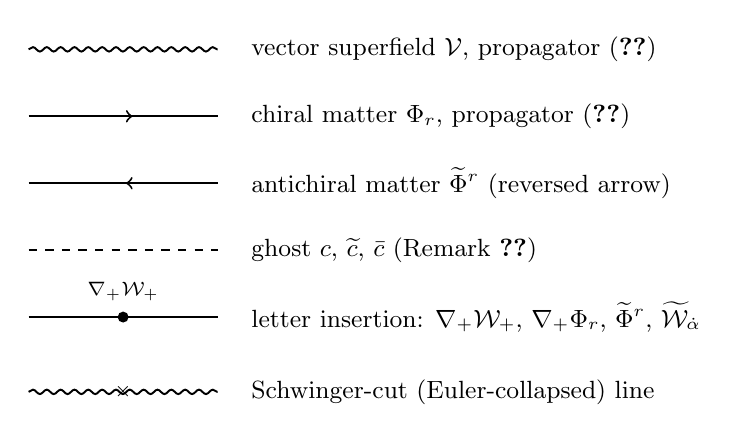
\begin{tikzpicture}
\draw[sV] (0,0) -- (2.4,0);
\node[right, font=\small] at (2.7,0)
  {vector superfield $\cV$, propagator \eqref{eq:ss:rules-propV}};
\draw[sPhi] (0,-0.85) -- (2.4,-0.85);
\node[right, font=\small] at (2.7,-0.85)
  {chiral matter $\Phi_{r}$, propagator \eqref{eq:ss:rules-propM}};
\draw[sPhit] (0,-1.7) -- (2.4,-1.7);
\node[right, font=\small] at (2.7,-1.7)
  {antichiral matter $\widetilde\Phi^{r}$ (reversed arrow)};
\draw[sghost] (0,-2.55) -- (2.4,-2.55);
\node[right, font=\small] at (2.7,-2.55)
  {ghost $c$, $\widetilde c$, $\bar c$ (Remark~\ref{rem:ss:rules-ghost})};
\draw[sleg] (0,-3.4) -- (1.2,-3.4)
  node[sinsert, label=above:{\scriptsize $\nabla_{+}\cW_{+}$}]{}
  -- (2.4,-3.4);
\node[right, font=\small] at (2.7,-3.4)
  {letter insertion: $\nabla_{+}\cW_{+}$, $\nabla_{+}\Phi_{r}$, $\widetilde\Phi^{r}$, $\bcW_{\dot\alpha}$};
\draw[sVcut] (0,-4.35) -- (2.4,-4.35);
\node[font=\scriptsize] at (1.2,-4.35) {$\times$};
\node[right, font=\small] at (2.7,-4.35)
  {Schwinger-cut (Euler-collapsed) line};
\end{tikzpicture}
\caption{Line-style legend for the supergraphs of this section. Wavy lines are vector-superfield propagators; solid lines with forward (reversed) arrows are chiral (antichiral) matter propagators; dashed lines are ghosts. A filled dot on an external leg is a letter insertion carrying its operator, while every uncontracted field pair becomes a propagator. A wavy line with an $\times$ mark is a Schwinger-cut (Euler-collapsed) line of the cutting mechanism of Section~\ref{sec:superspace:cutting}.}
\label{fig:ss:legend}
\end{figure}

The rules of this subsection feed every ordered channel: assembled channel by channel, they produce the seven nonzero families~\eqref{eq:ss:ch-bb}--\eqref{eq:ss:ch-dcb}, each with the common prefactor $-\frac{\h g^{2}}{16\sqrt2\,\pi^{2}}\,f^{ACD}f^{BCE}$, and the fifty-two structural zeros of the census. The comparison of these results with the holomorphic-twist alphabet is deferred to Section~\ref{sec:ht} \cite{BK}.

% sec04b-seed.tex — Section 4, expanded seed subsection.
% Writer: 作家_种子 (Writer_Seed). Body LaTeX only; macros live in main.tex.
% This file REPLACES the old short seed subsection. It is \input inside
% sec04-superspace.tex after the selection-rule subsection.

\subsection{The seed channel $(b,b)$: the complete one-loop computation}%
\label{sec:superspace:seed}

We now compute the seed channel $(b,b)$, the simplest nonzero channel and the
scale anchor of the whole table of Section~\ref{sec:superspace:table}, at full
granularity: the graph inventory with orientations, the Wick contraction
enumeration, the amplitude assembly, the $D$-algebra numerator chain, the
evanescent extraction, the pole cancellation, the loop integral, and the
restoration of the letter normalization, closing with the word-by-word
comparison against the holomorphic-twist result of~\cite{BK}. We fix once and
for all an orientation of the two field-strength insertions and a marked
internal line. The graph weights below are computed with unit-normalized
field-strength insertions $\nabla_+\cW_+$; the letter normalization
$b=-(i/\sqrt2)\nabla_+\cW_+$ is restored at the end.

\paragraph{1. Setup: the channel, the letters, and the marking conventions.}
The channel is the one-loop Schwinger--Dyson descent of the ordered composite
of two field-strength insertions,
\begin{equation}\label{eq:ss:seedchannel}
\nabla_{-}\Big(\nabla_{+}\cW_{+}^{A}\,\nabla_{+}\cW_{+}^{B}\Big),
\qquad
b^{A}=-\frac{i}{\sqrt2}\,\nabla_{+}\cW_{+}^{A},
\end{equation}
with the letter $b$ of Definition~\ref{def:ss:letters}. Both insertions are
Grassmann-even, so the Leibniz rule~\eqref{eq:ss:leibniz} contributes no sign
and splits the probe into two marked occurrences,
\begin{equation}\label{eq:ss:seedleibniz}
\nabla_{-}\Big(\nabla_{+}\cW_{+}^{A}\,\nabla_{+}\cW_{+}^{B}\Big)
=\big(\nabla_{-}\nabla_{+}\cW_{+}^{A}\big)\,\nabla_{+}\cW_{+}^{B}
+\nabla_{+}\cW_{+}^{A}\,\big(\nabla_{-}\nabla_{+}\cW_{+}^{B}\big) .
\end{equation}
These are two different marked occurrences, not a multiplicity of either one;
there is no factor $2$ from the source. We fix the ordered external data once
and for all: an antichiral background leg $\bcW^{D}(q)$ at the antichiral
cubic vertex $v_1$, a chiral background leg $\cW_{+}^{E}(p)$ at the chiral
cubic vertex $v_2$, and the composite source vertex $S$ carrying both
insertions and the $\nabla_{-}$ probe. All momenta are incoming
(Remark~\ref{rem:ss:nevercontract}), the loop momentum is $k$, and the three
internal edges are routed as
\begin{equation}\label{eq:ss:seedrouting}
r_0=k\quad(S\to v_1),\qquad
r_1=k+q\quad(v_1\to v_2),\qquad
r_2=k+p+q\quad(v_2\to S).
\end{equation}
There are exactly two ordered source attachments: the \emph{directed}
attachment, in which the insertion of color $A$ contracts toward the
antichiral vertex $v_1$ and the insertion of color $B$ toward the chiral
vertex $v_2$, and the \emph{reflected} attachment, in which they are
interchanged. The complete set of source/mark rows is
\begin{center}
\begin{tabular}{cccl}
\hline
source attachment & marked occurrence & rank-two evanescent numerator &
ordered output\\
\hline
$A\to\bcW,\ B\to\cW$ & $A$ & yes &
$\big\langle\bcW,\nabla_{+}\cW_{+}\big\rangle$\\
$A\to\bcW,\ B\to\cW$ & $B$ & no & none\\
$A\to\cW,\ B\to\bcW$ & $A$ & no & none\\
$A\to\cW,\ B\to\bcW$ & $B$ & yes &
$\big\langle\nabla_{+}\cW_{+},\bcW\big\rangle$\\
\hline
\end{tabular}
\end{center}
The two anomaly-bearing rows are the directed and the reflected term; they
are not two copies of either term. Reflection is a distinct ordered output
with weight one.

\paragraph{2. Graph inventory.}
There is exactly one gauge-sector graph topology at order $g^{2}$: the mixed-chirality
pure-gauge triangle, with one chiral cubic vertex, one antichiral cubic
vertex, the composite source vertex, and three internal vector-superfield
lines. With the canonically normalized prepotential
$u:=\cV/(\sqrt2\,g)$ and $[X,u]^{A}:=f^{ABC}X^{B}u^{C}$, the two cubic
actions generating the vertices are
\begin{equation}\label{eq:ss:seedcubic}
S_{+,3}=-\frac{g}{4}\int d^{8}z\;\cW^{A\alpha}\,[\cD_{\alpha}u,u]^{A},
\qquad
S_{-,3}=+\frac{g}{4}\int d^{8}z\;\bcW^{A}_{\dot\alpha}\,
[\bcD^{\dot\alpha}u,u]^{A}.
\end{equation}
The two ordered chiral assignments of the interaction expansion collapse:
\begin{equation}\label{eq:ss:seedactionorder}
\frac{1}{2!}\left(S_{+,3}S_{-,3}+S_{-,3}S_{+,3}\right)=S_{+,3}S_{-,3},
\end{equation}
so the action-order factor is exactly $1$. The two ordered parent triangles
are displayed in Figure~\ref{fig:ss:seedtriangles}.

\begin{figure}[t]
\centering
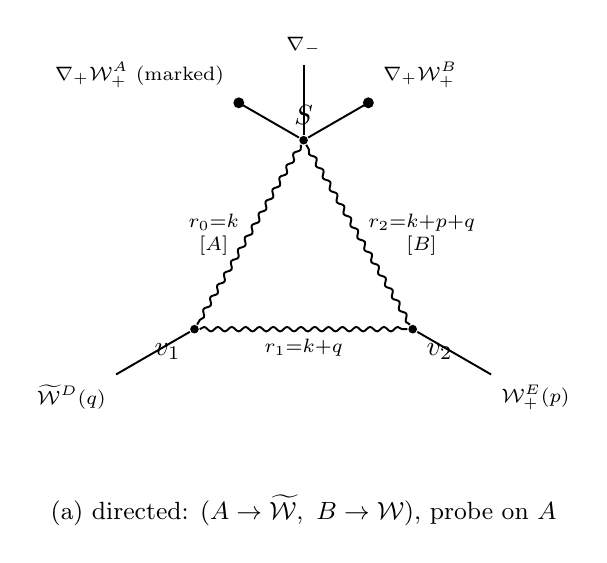
\begin{tikzpicture}
  \node[svertex, label=above:$S$] (S) at (90:1.6) {};
  \node[svertex, label=below left:$v_1$] (v1) at (210:1.6) {};
  \node[svertex, label=below right:$v_2$] (v2) at (330:1.6) {};
  \draw[sV] (S) to node[midway,left,align=center,font=\scriptsize]
        {$r_0{=}k$\\$[A]$} (v1);
  \draw[sV] (v1) to node[midway,below,font=\scriptsize] {$r_1{=}k{+}q$} (v2);
  \draw[sV] (v2) to node[midway,right,align=center,font=\scriptsize]
        {$r_2{=}k{+}p{+}q$\\$[B]$} (S);
  \draw[sleg] (v1) -- ++(210:1.15)
        node[below left,font=\scriptsize] {$\bcW^{D}(q)$};
  \draw[sleg] (v2) -- ++(330:1.15)
        node[below right,font=\scriptsize] {$\cW_{+}^{E}(p)$};
  \draw[sleg] (S) -- ++(150:0.95)
        node[sinsert,label={[font=\scriptsize]above left:%
        {$\nabla_{+}\cW_{+}^{A}$ (marked)}}] {};
  \draw[sleg] (S) -- ++(30:0.95)
        node[sinsert,label={[font=\scriptsize]above right:%
        {$\nabla_{+}\cW_{+}^{B}$}}] {};
  \draw[sleg] (S) -- ++(90:0.95) node[above,font=\scriptsize] {$\nabla_{-}$};
  \node[font=\small] at (0,-3.1) {(a) directed: $(A\to\bcW,\ B\to\cW)$,
        probe on $A$};
\end{tikzpicture}
\hspace{1.2em}
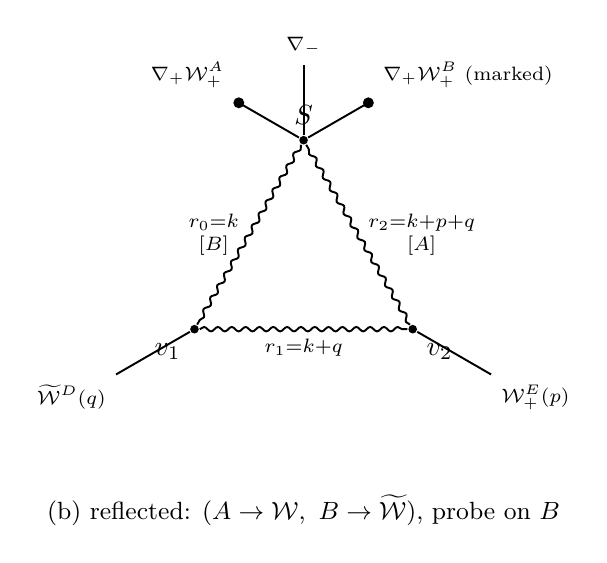
\begin{tikzpicture}
  \node[svertex, label=above:$S$] (S) at (90:1.6) {};
  \node[svertex, label=below left:$v_1$] (v1) at (210:1.6) {};
  \node[svertex, label=below right:$v_2$] (v2) at (330:1.6) {};
  \draw[sV] (S) to node[midway,left,align=center,font=\scriptsize]
        {$r_0{=}k$\\$[B]$} (v1);
  \draw[sV] (v1) to node[midway,below,font=\scriptsize] {$r_1{=}k{+}q$} (v2);
  \draw[sV] (v2) to node[midway,right,align=center,font=\scriptsize]
        {$r_2{=}k{+}p{+}q$\\$[A]$} (S);
  \draw[sleg] (v1) -- ++(210:1.15)
        node[below left,font=\scriptsize] {$\bcW^{D}(q)$};
  \draw[sleg] (v2) -- ++(330:1.15)
        node[below right,font=\scriptsize] {$\cW_{+}^{E}(p)$};
  \draw[sleg] (S) -- ++(150:0.95)
        node[sinsert,label={[font=\scriptsize]above left:%
        {$\nabla_{+}\cW_{+}^{A}$}}] {};
  \draw[sleg] (S) -- ++(30:0.95)
        node[sinsert,label={[font=\scriptsize]above right:%
        {$\nabla_{+}\cW_{+}^{B}$ (marked)}}] {};
  \draw[sleg] (S) -- ++(90:0.95) node[above,font=\scriptsize] {$\nabla_{-}$};
  \node[font=\small] at (0,-3.1) {(b) reflected: $(A\to\cW,\ B\to\bcW)$,
        probe on $B$};
\end{tikzpicture}
\caption{The two ordered parent triangles of the seed channel $(b,b)$. Each
triangle has the composite source vertex $S$ carrying the two letter
insertions (filled dots) and the $\nabla_{-}$ probe leg, the antichiral cubic
vertex $v_1$ with external leg $\bcW^{D}(q)$, the chiral cubic vertex $v_2$
with external leg $\cW_{+}^{E}(p)$, and three internal vector-superfield
lines (wavy) with edge momenta $r_0=k$, $r_1=k+q$, $r_2=k+p+q$. The bracket
$[A]$/$[B]$ on an edge records which source color contracts toward that
vertex. (a) The directed orientation, with the probe on the $A$ occurrence.
(b) The reflected orientation, with the probe on the $B$ occurrence.}
\label{fig:ss:seedtriangles}
\end{figure}

For each marked occurrence, the Schwinger cut of
Section~\ref{sec:superspace:cutting} collapses the internal edge carrying the
marked line: the occurrence probed at the $v_1$-side port collapses the edge
$e_0$ with momentum $r_0$, and the occurrence probed at the $v_2$-side port
collapses the edge $e_2$ with momentum $r_2$. For one marked edge the row
count is
\begin{equation}\label{eq:ss:seedcontactcount}
\frac{1}{2!}\cdot 2_{\text{action orderings}}\cdot
2_{\text{Wick endpoints}}=2\ \text{endpoint rows},
\end{equation}
so there are exactly four occurrence-resolved Schwinger contact rows in total
(two cut edges times two Wick endpoints). The contact topology is displayed
in Figure~\ref{fig:ss:seedcontact}.

\begin{figure}[t]
\centering
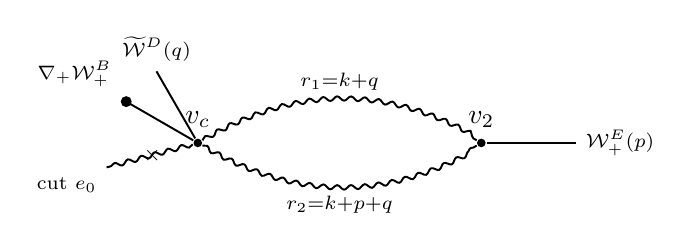
\begin{tikzpicture}
  \node[svertex, label=above:$v_c$] (vc) at (0,0) {};
  \node[svertex, label=above:$v_2$] (v2) at (3.6,0) {};
  \draw[sV, bend left=30] (vc) to node[midway,above,font=\scriptsize]
        {$r_1{=}k{+}q$} (v2);
  \draw[sV, bend right=30] (vc) to node[midway,below,font=\scriptsize]
        {$r_2{=}k{+}p{+}q$} (v2);
  % sVcut rendering: main.tex's sVcut (snake + markings postaction) triggers a
  % PGF ``Dimension too large'' error under pgf 3.1.10, so the identical cut-line
  % rendering is drawn here as an sV wavy line with an explicit $\times$ marker.
  \draw[sV] (vc) -- ++(195:1.2) coordinate (cutend);
  \node[font=\scriptsize] at ($(vc)!0.5!(cutend)$) {$\times$};
  \node[below left,font=\scriptsize] at (cutend) {cut $e_0$};
  \draw[sleg] (vc) -- ++(150:1.05)
        node[sinsert,label={[font=\scriptsize]above left:%
        {$\nabla_{+}\cW_{+}^{B}$}}] {};
  \draw[sleg] (vc) -- ++(120:1.05)
        node[above,font=\scriptsize] {$\bcW^{D}(q)$};
  \draw[sleg] (v2) -- ++(0:1.2)
        node[right,font=\scriptsize] {$\cW_{+}^{E}(p)$};
\end{tikzpicture}
\caption{The Schwinger contact (cut) topology of the seed channel. Cutting
the marked edge $e_0$ collapses the source vertex $S$ and the antichiral
vertex $v_1$ into the single contact vertex $v_c$: the probed occurrence
$\nabla_{-}(\nabla_{+}\cW_{+}^{A})$ has become the Euler-operator insertion
that collapses the $e_0$ line (wavy with $\times$), while the unmarked
insertion $\nabla_{+}\cW_{+}^{B}$ and the external leg $\bcW^{D}(q)$ remain
at $v_c$. Two internal vector lines with momenta $r_1=k+q$ and $r_2=k+p+q$
run from $v_c$ to the chiral vertex $v_2$. The $e_2$ family is the mirror
image, with contact vertex $v_c=S\sqcup v_2$ and internal lines $r_0$ and
$r_1$. With the two Wick port rows per edge this gives the four
occurrence-resolved contact rows of paragraph~7.}
\label{fig:ss:seedcontact}
\end{figure}

Every remaining order-$g^{2}$ orbit vanishes exactly in the anomaly sector.
The spectator self-energy insertions, the one-cubic-vertex bubbles, and the
quartic seagull obey
\begin{align}
\big\langle I_2\big\rangle_0 &= 0
&&\text{(source-quadratic self-energy: its only denominator is $k^{2}$,
hence a scaleless tadpole),}\notag\\
-\frac{1}{\h}\big\langle I_1S_{g3}\big\rangle_0 &= 0
&&\text{(one-cubic bubble: numerator trace }\ \operatorname{tr}_4 H=2-2=0
\text{),}\label{eq:ss:seedorbits}\\
-\frac{1}{\h}\big\langle I_0S_{g4}\big\rangle_0 &= 0
&&\text{(quartic seagull: }\ \operatorname{tr}_4 H_4=-4+4=0\text{),}\notag
\end{align}
so only the two-cubic triangle
$(2\h^{2})^{-1}\langle I_0S_{g3}S_{g3}\rangle_0$ of
Figure~\ref{fig:ss:seedtriangles} and its Schwinger cuts survive. The matter
orbits $I_2$, $I_1S_{m3}$, $I_0S_{m4}$ vanish in the same way; the matter
triangle of the same channel is evaluated in paragraph~9.

\paragraph{3. Wick contractions.}
The three internal lines are vector-superfield contractions with propagator
\begin{equation}\label{eq:ss:seeduprop}
\big\langle u^{A}(p,1)\,u^{B}(-p,2)\big\rangle
=-\frac{\h\,\delta^{AB}}{p^{2}}\,\delta^{4}(\theta_1-\theta_2),
\end{equation}
with the Killing form normalized to $\kappa_{AB}=\delta_{AB}$. The two cubic
vertices each supply two quantum-port assignments through the derivative
differences of their second variations, the Hessians
\begin{equation}\label{eq:ss:seedhess}
H_{\cW}=+\frac{ig}{4}\,f^{UCE}\,\cW^{E\gamma}
\big(\cD_{C\gamma}-\cD_{U\gamma}\big),
\qquad
H_{\bcW}=-\frac{ig}{4}\,f^{UCD}\,\bcW^{D}_{\dot\gamma}
\big(\bcD_{C}{}^{\dot\gamma}-\bcD_{U}{}^{\dot\gamma}\big).
\end{equation}
The labeled double variation is
\begin{equation}\label{eq:ss:seedports}
\delta_1\delta_2[\cD u,u]=[\cD u_1,u_2]+[\cD u_2,u_1],
\end{equation}
whose two summands are the port rows $(S,B)$ and $(B,S)$ --- the row in which
the first, respectively the second, quantum port carries the source role.
The second variation already contains the two labeled quantum-port
assignments, so no $2!$ from the equal Hessians remains. For one fixed
directed source attachment the port-preserving Wick factor is likewise $1$:
the two rows are equal by relabeling of the Gaussian integral and sum against
the $1/2!$ of the second variation, giving the Wick weight
\begin{equation}\label{eq:ss:wick}
w_{\mathrm{Wick}}=\frac{1}{2!}(1+1)=1 .
\end{equation}

\begin{remark}[Granularity of the contraction enumeration]%
\label{rem:ss:seedwick}
The enumeration above is organized by the quantum-role rows $(S,B),(B,S)$
and by the derivative endpoint pairs $(r_i,r_j)$; a field-by-field pairing
picture of the individual $u$ fields is not used at any step. The endpoint
content is not multiplied after the two Hessians are expanded: no endpoint
row acquires an additional factor.
\end{remark}

\paragraph{4. Amplitude assembly.}
The linearized unit insertion and its probed descendant are
\begin{equation}\label{eq:ss:seedinsert}
K_{+}^{c}:=-\frac{1}{4\sqrt2}\,\cD_{+}\bcD^{2}\cD_{+},
\qquad
\nabla_{-}K_{+}^{c}
=-\frac{1}{4\sqrt2}\,\cD_{-}\cD_{+}\bcD^{2}\cD_{+}
=-\frac{1}{8\sqrt2}\,\cD^{2}\bcD^{2}\cD_{+},
\end{equation}
where on the internal lines the frame derivatives act as their flat
counterparts $\cD_\pm$, $\bcD_{\dot\pm}$ and we used the spinor-derivative
square move
\begin{equation}\label{eq:ss:seedDmoves}
\cD^{2}=2\,\cD_{-}\cD_{+},
\qquad
\bcD^{2}=2\,\bcD_{\dot+}\bcD_{\dot-}.
\end{equation}
After the three contractions, the unmarked leg retains the residual operator
$K_{+}^{c}$ and the probed leg retains $\nabla_{-}K_{+}^{c}$; their numerical
product is
\begin{equation}\label{eq:ss:seedinsertfactor}
\left(-\frac{1}{8\sqrt2}\right)\left(-\frac{1}{4\sqrt2}\right)=\frac{1}{64}.
\end{equation}
The vertex (exponent) Hessians of~\eqref{eq:ss:seedhess}, including the
$1/\h$ of each interaction vertex, are
\begin{equation}\label{eq:ss:seedvhess}
\widehat H_{\cW}=-\frac{ig}{4\h}\,f^{UCE}\,\cW^{E\gamma}
\big(\cD_{C\gamma}-\cD_{U\gamma}\big),
\qquad
\widehat H_{\bcW}=+\frac{ig}{4\h}\,f^{UCD}\,\bcW^{D}_{\dot\gamma}
\big(\bcD_{C}{}^{\dot\gamma}-\bcD_{U}{}^{\dot\gamma}\big),
\end{equation}
and assembling them with the three propagators~\eqref{eq:ss:seeduprop} gives
\begin{equation}\label{eq:ss:seedassembly}
\left(-\frac{ig}{4\h}\right)\left(+\frac{ig}{4\h}\right)(-\h)^{3}
=\frac{g^{2}}{16\h^{2}}\,(-\h^{3})
=-\frac{\h g^{2}}{16}.
\end{equation}
The three Killing deltas of the propagators reduce the color factor of the
two Hessians, with the source colors attached per the fixed orientation, to
\begin{equation}\label{eq:ss:seedcolor}
f^{UCD}f^{U'C'E}\,\delta_{UU'}\delta_{CC'}
\;\longrightarrow\;
f^{ACD}f^{BCE}
\qquad(\text{sum over }C).
\end{equation}

\begin{remark}[Two equivalent normalization frames]\label{rem:ss:seedframes}
Equation~\eqref{eq:ss:seedassembly} is the canonical-letter bookkeeping:
vertex magnitudes $g/(4\h)$, propagators $-\h$, and the explicit insertion
factor $1/64$ of~\eqref{eq:ss:seedinsertfactor}. In the unit-insertion frame
used for the remaining steps the same graph weight is organized with the
ordered cubic vertex factors
\begin{equation}\label{eq:ss:vertices}
\left(+\frac{ig}{2}\right)\left(-\frac{ig}{2}\right)=\frac{g^{2}}{4}
\end{equation}
and the $D$-algebra weight $w_D$ of~\eqref{eq:ss:dweight} below. The two
bookkeepings describe the same graph weight: in the canonical frame the
vertex factor sits inside $-\h g^{2}/16$, in the unit-insertion frame inside
$g^{2}/4$, the difference being the propagator rescaling
$u=\cV/(\sqrt2\,g)$ on the three internal lines together with the insertion
rescaling. Each cubic vertex carries $\h^{-1}$ and each of the three
propagators carries $\h$, leaving the net one-loop power $\h$.
\end{remark}

\paragraph{5. The $D$-algebra numerator chain.}
For the fixed orientation the covariant spinor numerator is the chain
\begin{equation}\label{eq:ss:seedspinchain}
N_{G,+}{}^{\dot\alpha}
=(r_0+r_1)_{+\dot\beta}\,(ip)^{\dot\beta\gamma}\,
(r_1+r_2)_{\gamma}{}^{\dot\alpha},
\qquad
T_{m\rho n,+}{}^{\dot\alpha}
:=(\sigma_m\bar\sigma_\rho\sigma_n)_{+}{}^{\dot\alpha},
\end{equation}
where the explicit $i$ is tied to the locked dotted-index convention
$k_{+}^{\dot0}=\sigma_E(k)_{0\dot1}$,
$k_{+}^{\dot1}=-\sigma_E(k)_{0\dot0}$; in the opposite convention the same
covariant chain is written with $p^{\dot\beta\gamma}$ and no explicit $i$.
The $D^{2}/\bcD^{2}$ moves of~\eqref{eq:ss:seedDmoves} put the marked
insertion into the form $-\frac{1}{8\sqrt2}\cD^{2}\bcD^{2}\cD_{+}$ displayed
in~\eqref{eq:ss:seedinsert}. The loop is saturated by the identity
\begin{equation}\label{eq:ss:seedsat}
\delta^{4}(\theta_{12})\,\cD^{2}\bcD^{2}\,\delta^{4}(\theta_{12})
=16\,\delta^{4}(\theta_{12})
\end{equation}
of Section~\ref{sec:gaugebv}, and the two mixed anticommutators
\begin{equation}\label{eq:ss:seedmixed}
\{\cD,\bcD\}=2\,\sigma\!\cdot\!p
\end{equation}
contribute one factor $2$ each, so the $D$-algebra content of the closed
loop is
\begin{equation}\label{eq:ss:seeddalg}
\left(\frac{1}{64}\right)(16)(2)(2)=1 .
\end{equation}
This is a $D$-algebra factor; it is not four additional Wick contractions.
Equivalently, in the unit-insertion frame the closed-loop mixed $D$-algebra
weight is
\begin{equation}\label{eq:ss:dweight}
w_D=\frac{1}{32}\cdot16\cdot2\cdot2=2 ,
\end{equation}
where the $1/32$ is the insertion normalization of that frame and the $16$
is the loop-saturation identity~\eqref{eq:ss:seedsat}. The total prefactor
before the loop integral is therefore
\begin{equation}\label{eq:ss:prefactor}
w_{\mathrm{Wick}}\,\frac{g^{2}}{4}\,w_D
=1\cdot\frac{g^{2}}{4}\cdot2=\frac{g^{2}}{2} .
\end{equation}
The four derivative endpoint rows of one cut word, with their raw and
transport signs, are
\begin{align}
(r_0,r_1):&\quad (-1)(-1)=+1,\notag\\
(r_0,r_2):&\quad (+1)(+1)=+1,\label{eq:ss:seedsigntable}\\
(r_1,r_1):&\quad (+1)(+1)=+1,\notag\\
(r_1,r_2):&\quad (-1)(-1)=+1,\notag
\end{align}
and the closed word carries in addition the single odd source-loop
integration-by-parts sign $s_{\mathrm{global}}=-1$, so the signed row weight
is
\begin{equation}\label{eq:ss:seedrowsign}
w_{T,\mathrm{rows}}
=s_{\mathrm{global}}\left(\frac{1}{64}\right)(16)(2)(2)=(-1)(1)=-1,
\qquad
\left(-\frac{\h g^{2}}{16}\right)w_{T,\mathrm{rows}}=+\frac{\h g^{2}}{16}.
\end{equation}
The rank-two finite spinor word is reduced by the four-dimensional identity
\begin{equation}\label{eq:ss:seedfierz}
\sigma\!\cdot\!L\,\bar\sigma\!\cdot\!p\,\sigma\!\cdot\!L
=2(L\!\cdot\!p)\,\sigma\!\cdot\!L-\bar L^{2}\,\sigma\!\cdot\!p ,
\end{equation}
whose two factors of $2L$ give
$4\,\sigma\!\cdot\!L\,\bar\sigma\!\cdot\!p\,\sigma\!\cdot\!L
=8(L\!\cdot\!p)\,\sigma\!\cdot\!L-4\bar L^{2}\,\sigma\!\cdot\!p$; the first
term belongs to the full-$d$ Schwinger-exact tensor reduction, and the
selected inverse-square parent and its cut differ by
\begin{equation}\label{eq:ss:seedsigmafour}
-4\big(\bar L^{2}-L_d^{2}\big)\,\sigma\!\cdot\!p
=-4\,\mul^{2}\,\sigma\!\cdot\!p ,
\end{equation}
which vanishes identically if $\bar L^{2}$ is replaced by $L_d^{2}$ before
the cut subtraction. For the reflected ordering the dotted-index reordering
gives
\begin{equation}\label{eq:ss:seedreflect}
\big(\partial^{\dot\alpha}\,\nabla_{+}\cW_{+}^{D}\big)\,\bcW_{\dot\alpha}^{E}
=-\,\big(\partial_{\dot\alpha}\,\nabla_{+}\cW_{+}^{D}\big)\,
\bcW^{E\dot\alpha},
\end{equation}
one minus sign per reordering, which is the origin of the antisymmetric
ordered pair of outputs. The exact marked words behind the endpoint table
are
\begin{equation}\label{eq:ss:seedGwords}
\mathcal G_1=(b_{0+}+b_{1+})\,W_{02},
\qquad
\mathcal G_2=(b_{0+}-b_{1+})\,W_{02},
\qquad
W_{02}=r_{0+}\wedge r_{2+},
\end{equation}
with $b_{0+}-b_{1+}=q_{+\dot-}$ purely external, so $\mathcal G_2$ has no
rank-two loop component (the rows marked ``no'' in the table of
paragraph~1), while $b_{0+}+b_{1+}=2L_{+\dot-}+\text{external}$ is rank two
(the rows marked ``yes'').

\begin{remark}[Status of the sign table]\label{rem:ss:seedsigns}
The endpoint-row assignment~\eqref{eq:ss:seedsigntable} and the global sign
$s_{\mathrm{global}}=-1$ are recorded primitives of the computation: no
independent human-readable noncommutative $D$-algebra trace emitting them is
quoted here. They are superseded in effect by the exact exterior-algebra
words~\eqref{eq:ss:seedGwords} and by the machine replays of
Remark~\ref{rem:ss:seedchecks}, which confirm the full factor chain with
zero failures.
\end{remark}

\paragraph{6. Evanescent extraction and tensor reduction.}
On every marked line $e$ of every one-loop graph the cutting-failure
identity~\eqref{eq:ss:cuttingfailure} isolates one universal insertion:
\begin{equation}\label{eq:ss:seededge}
\frac{\bar r_e^{\,2}}{D_0D_1D_2}-\frac{1}{\prod_{j\ne e}D_j}
=\frac{\mul^{2}}{D_0D_1D_2},
\end{equation}
with $D_i=r_{i,d}^{2}$; replacing $\bar r_e^{\,2}$ by $r_{e,d}^{\,2}$ before
the subtraction makes the expression identically zero and removes the
anomaly. With $D_0=\ell^{2}$, $D_1=(\ell+p)^{2}$, $D_2=(\ell+p+q)^{2}$, the
ordered Feynman parametrization is
\begin{equation}\label{eq:ss:feynman}
\frac{1}{D_0D_1D_2}
=2\!\int_{x,y,z\geq0}\!dx\,dy\,dz\;\delta(1-x-y-z)\,\frac{1}{(r^{2}+\Delta)^{3}},
\qquad
\int_{x,y,z\geq0}\!dx\,dy\,dz\;\delta(1-x-y-z)=\frac12 ,
\end{equation}
with the shift, writing $Q=p+q$,
\begin{equation}\label{eq:ss:seedshift}
\ell=k+yq+zQ,
\qquad
\Delta=xyq^{2}+xzQ^{2}+yzp^{2}.
\end{equation}
The two numerator legs $L_1=2k+q$ and $L_2=2k+p+2q$ become
\begin{equation}\label{eq:ss:seedL12}
L_1=2\ell+(1-2y)q-2zQ,
\qquad
L_2=2\ell+(1-2y)q+(1-2z)Q,
\end{equation}
so the odd-$\ell$ terms integrate to zero and only the $\ell_m\ell_n$ piece
survives. Hatted rotational reduction and~\eqref{eq:ss:Jnidentities} give
\begin{equation}\label{eq:ss:tensorreduction}
\int_r\frac{r_mr_n}{(r^{2}+\Delta)^{3}}
=\frac{\widehat\delta_{mn}}{d}\,(J_2-\Delta J_3)
=\frac{\widehat\delta_{mn}}{4}\,J_2 ,
\end{equation}
the $\tfrac14$ being exact since
$(1-\tfrac{\epsilon}{2})/(4-2\epsilon)=\tfrac14$ identically in $\epsilon$.
Consequently the pole part of the parent triangle with numerator legs
$L_1^{m}L_2^{n}$ is
\begin{equation}\label{eq:ss:pole}
\operatorname*{Pole}_{\epsilon=0}
\int_{\ell}\frac{L_1^{m}L_2^{n}}{D_0D_1D_2}
=\frac{\widehat\delta^{mn}}{16\pi^{2}\epsilon} .
\end{equation}
Assembling the prefactor~\eqref{eq:ss:prefactor}, the simplex
factor~\eqref{eq:ss:feynman}, the residue~\eqref{eq:ss:pole}, and the spinor
chain $\sigma_m\bar\sigma_\rho\sigma_n$ contracted with the hatted external
momentum $p^{\rho}$, the parent triangle pole is
\begin{equation}\label{eq:ss:parentpole}
\Gamma_{T}
=\frac{\h g^{2}}{32\pi^{2}\epsilon}\,
f^{ACD}f^{BCE}\,\widehat\delta^{mn}\,
\sigma_m\bar\sigma_\rho\sigma_n\,p^{\rho} .
\end{equation}

\paragraph{7. Schwinger contact rows.}
The four occurrence-resolved contact rows of
Figure~\ref{fig:ss:seedcontact} are
\begin{center}
\begin{tabular}{ccll}
\hline
row & cut edge & marked occurrence & Wick port row\\
\hline
$j=1$ & $e_0$ & $\nabla_{-}(\nabla_{+}\cW_{+}^{A})$ & $(S,B)$\\
$j=2$ & $e_0$ & $\nabla_{-}(\nabla_{+}\cW_{+}^{A})$ & $(B,S)$\\
$j=3$ & $e_2$ & $\nabla_{+}\cW_{+}^{A}\,\nabla_{-}(\nabla_{+}\cW_{+}^{B})$
& $(S,B)$\\
$j=4$ & $e_2$ & $\nabla_{+}\cW_{+}^{A}\,\nabla_{-}(\nabla_{+}\cW_{+}^{B})$
& $(B,S)$\\
\hline
\end{tabular}
\end{center}
and each row carries the same sign chain
\begin{equation}\label{eq:ss:signchain}
\left(-\frac14\right)_{\mathrm{cut}}
(-1)_{\mathrm{endpoint}}
\left(\frac12\right)_{\nabla_{-}\nabla_{+}=\nabla^{2}/2}
(2)_{\mathrm{mixed}}
(2)_{\mathrm{Wick}}
\left(-\frac12\right)_{p_{+}}
=-\frac14 ,
\end{equation}
whose factors are, in order: the cut/insertion coefficient, the endpoint
transport sign, the spinor-derivative square
move~\eqref{eq:ss:seedDmoves}, the mixed anticommutator
factor~\eqref{eq:ss:seedmixed}, the two Wick endpoints, and the plus-frame
momentum projection. There is no extra edge factor $2$ and no metric-trace
factor $d$ or $4$ on the contact side. A single row gives
\begin{equation}\label{eq:ss:singlerow}
\Gamma_{C,j}
=-\frac14\cdot\frac{\h g^{2}}{2}\cdot\frac{1}{16\pi^{2}\epsilon}\,
f^{ACD}f^{BCE}\,\delta_4^{mn}\,
\sigma_m\bar\sigma_\rho\sigma_n\,p^{\rho}
=-\frac{\h g^{2}}{128\pi^{2}\epsilon}\,
f^{ACD}f^{BCE}\,\delta_4^{mn}\,
\sigma_m\bar\sigma_\rho\sigma_n\,p^{\rho} ,
\end{equation}
and the four occurrence-resolved rows sum to
\begin{equation}\label{eq:ss:contactrows}
\Gamma_{C}
=\sum_{j=1}^{4}\Gamma_{C,j}
=-\frac{\h g^{2}}{32\pi^{2}\epsilon}\,
f^{ACD}f^{BCE}\,\delta_4^{mn}\,
\sigma_m\bar\sigma_\rho\sigma_n\,p^{\rho} .
\end{equation}

\paragraph{8. Pole cancellation and the $-2\epsilon$ trace.}
The four-dimensional metric parts of~\eqref{eq:ss:parentpole}
and~\eqref{eq:ss:contactrows} cancel exactly: since
$\widehat\delta^{mn}-\delta_4^{mn}=-\breve\delta^{mn}$,
\begin{equation}\label{eq:ss:polecancel}
\Gamma_{T}+\Gamma_{C}
=-\frac{\h g^{2}}{32\pi^{2}\epsilon}\,
f^{ACD}f^{BCE}\,\breve\delta^{mn}\,
\sigma_m\bar\sigma_\rho\sigma_n\,p^{\rho} ,
\end{equation}
a pure evanescent numerator, precisely as in the bookkeeping principle of
Remark~\ref{rem:ss:polebookkeeping}. The external momentum is hatted, so
contracting with $p^{\rho}$ first and using $\breve\delta\,p=0$ and
$\breve\delta^{mn}\bar\sigma_m\sigma_n=\breve\delta^{m}{}_{m}=2\epsilon$
with the four-dimensional spin algebra~\eqref{eq:ss:sigmaalgebra},
\begin{equation}\label{eq:ss:sigmatrace}
p^{\rho}\,\breve\delta^{mn}\,\sigma_m\bar\sigma_\rho\sigma_n
=2p^{\rho}\breve\delta_{\rho}{}^{n}\sigma_n
-p^{\rho}\sigma_\rho\,\breve\delta^{mn}\bar\sigma_m\sigma_n
=0-(\breve\delta^{m}{}_{m})\,p^{\rho}\sigma_\rho
=-2\epsilon\,p^{\rho}\sigma_\rho .
\end{equation}

\paragraph{9. The loop integral and the complete unit-insertion result.}
The shifted coefficient is independent of the simplex parameters, so
$2\int_{\Sigma_2}1=2(\tfrac12)=1$ by~\eqref{eq:ss:feynman}. Substituting
\eqref{eq:ss:sigmatrace} into~\eqref{eq:ss:polecancel} and using the
evanescent master integral~\eqref{eq:ss:masterintegral},
\begin{equation}\label{eq:ss:seedfinal}
\Gamma_{T}+\Gamma_{C}
=-\frac{\h g^{2}}{32\pi^{2}\epsilon}\,(-2\epsilon)\,
f^{ACD}f^{BCE}\,\sigma_\rho p^{\rho}
=\frac{\h g^{2}}{16\pi^{2}}\,
f^{ACD}f^{BCE}\,\sigma\!\cdot\!p .
\end{equation}
The $\sigma$-chain trace forces the position-space output to be a dotted
bilinear of the form~\eqref{eq:ss:bilinear}: this is the output structure
quoted as grading (iv) in Section~\ref{sec:superspace:selection}. The
directed triangle emits the ordered word
$\langle\bcW^{D},\nabla_{+}\cW_{+}^{E}\rangle$; the reflected triangle emits
the reordered word with the minus sign of~\eqref{eq:ss:seedreflect}; the two
words in which the holomorphic momentum acts along the $q$-leg are total
derivatives (equation-of-motion carriers) and drop out of the physical
output. The gauge sector of the channel is therefore
\begin{equation}\label{eq:ss:seedgauge}
\Gamma^{(1)}_{(b,b),\mathrm{gauge}}
=\frac{\h g^{2}}{16\pi^{2}}\,f^{ACD}f^{BCE}\,
\big\{\big\langle\bcW,\nabla_{+}\cW_{+}\big\rangle
-\big\langle\nabla_{+}\cW_{+},\bcW\big\rangle\big\}^{DE} .
\end{equation}
The matter sector of the same channel is the two-$\widetilde\Phi\cV\Phi$
marked triangle. Its two marked placements give, with the same master
integral~\eqref{eq:ss:masterintegral},
\begin{align}
4\h g^{2}\left(\frac23\right)\left(\frac{1}{32\pi^{2}}\right)
&=\frac{\h g^{2}}{12\pi^{2}},
\label{eq:ss:seedmatterone}\\
4\h g^{2}\left(-\frac16\right)\left(\frac{1}{32\pi^{2}}\right)
&=-\frac{\h g^{2}}{48\pi^{2}},
\label{eq:ss:seedmattertwo}
\end{align}
and the two placements sum to
\begin{equation}\label{eq:ss:seedmatternet}
\frac{\h g^{2}}{12\pi^{2}}-\frac{\h g^{2}}{48\pi^{2}}
=\frac{3\,\h g^{2}}{48\pi^{2}}
=\frac{\h g^{2}}{16\pi^{2}},
\end{equation}
carried by the matter words
$\sum_r\big(\langle\nabla_{+}\Phi_r,\widetilde\Phi^{r}\rangle
-\langle\widetilde\Phi^{r},\nabla_{+}\Phi_r\rangle\big)$. Collecting the
gauge sector~\eqref{eq:ss:seedgauge} and the matter
sector~\eqref{eq:ss:seedmatternet}, the complete channel in unit insertions
is
\begin{equation}\label{eq:ss:seedunitresult}
\begin{aligned}
\nabla_{-}\Big(\nabla_{+}\cW_{+}^{A}\,\nabla_{+}\cW_{+}^{B}\Big)
\Big|_{\text{1-loop}}
=\frac{\h g^{2}}{16\pi^{2}}\,f^{ACD}f^{BCE}\,
\Big\{&\big\langle\bcW,\nabla_{+}\cW_{+}\big\rangle
-\big\langle\nabla_{+}\cW_{+},\bcW\big\rangle\\
+&\sum_{r=1}^{3}\Big(
\big\langle\nabla_{+}\Phi_r,\widetilde\Phi^{r}\big\rangle
-\big\langle\widetilde\Phi^{r},\nabla_{+}\Phi_r\big\rangle\Big)
\Big\}^{DE} ,
\end{aligned}
\end{equation}
with the dotted contraction of~\eqref{eq:ss:bilinear} understood in each
bilinear.

\begin{remark}[The matter source-orientation sign]\label{rem:ss:seedmatter}
The relative size of the two matter placements in~\eqref{eq:ss:seedmatterone}
and~\eqref{eq:ss:seedmattertwo} is exact; the overall matter
source-orientation sign is fixed by the target-blind primitive-sign chain
($\eta_{\mathrm{src}}=+1$), giving the word order displayed
in~\eqref{eq:ss:seedunitresult}. The same sign is consistent with the
accepted component bottom projection of Section~\ref{sec:component} (an exact
projection of the superfield result, not an independent derivation) and is
checked independently by the holomorphic-twist comparison of paragraph~11.
\end{remark}

\paragraph{10. Restoring the letter normalization: the boxed result.}
The letters of Definition~\ref{def:ss:letters} give the substitutions
\begin{align}
\nabla_{+}\cW_{+}&=i\sqrt2\,b,
&\big(\nabla_{+}\cW_{+}^{A}\big)\big(\nabla_{+}\cW_{+}^{B}\big)
&=(i\sqrt2)^{2}\,b^{A}b^{B}=-2\,b^{A}b^{B},
\label{eq:ss:seedlettersub}\\
\big\langle\bcW,\nabla_{+}\cW_{+}\big\rangle
&=\big\langle-i\,\partial c,\,i\sqrt2\,b\big\rangle
=\sqrt2\,\big\langle\partial c,b\big\rangle,
&\big\langle\nabla_{+}\Phi_r,\widetilde\Phi^{r}\big\rangle
&=\big\langle\sqrt2\,\beta_r,\gamma^{r}\big\rangle
=\sqrt2\,\big\langle\beta_r,\gamma^{r}\big\rangle ,
\label{eq:ss:seedwordsub}
\end{align}
so that dividing~\eqref{eq:ss:seedunitresult} by the insertion factor $-2$
yields
\begin{equation}\label{eq:ss:seednetletter}
\nabla_{-}\big(b^{A}b^{B}\big)
=\frac{1}{-2}\cdot\sqrt2\cdot\frac{\h g^{2}}{16\pi^{2}}\,
f^{ACD}f^{BCE}\,\{\cdots\}
=-\frac{\h g^{2}}{16\sqrt2\,\pi^{2}}\,f^{ACD}f^{BCE}\,\{\cdots\} .
\end{equation}
Equivalently, in the bookkeeping of the unit-insertion frame: the two
insertions contribute a factor $(-i/\sqrt2)^{2}=-\tfrac12$ relative to the
unit field-strength normalization used above, while the output bilinears of
the seed channel contribute $\sqrt2$ in the alphabet of
Definition~\ref{def:ss:letters}, giving the net prefactor
$-\tfrac12\cdot\sqrt2\cdot\tfrac{\h g^2}{16\pi^2}
=-\tfrac{\h g^{2}}{16\sqrt2\,\pi^{2}}$. The position-space identity reads
\begin{equation}\label{eq:ss:bbresult}
\boxed{\;
\nabla_{-}\big(b^{A}b^{B}\big)
=-\frac{\h g^{2}}{16\sqrt2\,\pi^{2}}\,
f^{ACD}f^{BCE}\,
\Big\{
\langle\partial c,b\rangle-\langle b,\partial c\rangle
+\sum_{r=1}^{3}\big(
\langle\beta_{r},\gamma^{r}\rangle-\langle\gamma^{r},\beta_{r}\rangle
\big)\Big\}^{DE} .\;}
\end{equation}

\begin{remark}[Independent machine cross-checks]\label{rem:ss:seedchecks}
The factor chain of this subsection was replayed externally on $269$ external
slot assignments with zero failures, and on the full color mask ($9216$
entries, with a sparse replay of $2048$) with zero equality failures.
\end{remark}

\paragraph{11. The holomorphic-twist comparison for this channel.}
Budzik and Kulp compute the same channel in the holomorphic twist; their
zero-derivative display \cite[eq.~(3.64)]{BK} is
\begin{equation}\label{eq:ss:seedbk}
Q_1(b^A b^B)
=\kappa^{2} f_{ACD}f_{BCE} \left[
\partial_{\dot\alpha} c^D \partial^{\dot\alpha} b^E
-\partial_{\dot\alpha} b^D\partial^{\dot\alpha} c^E
+\partial_{\dot\alpha}(\beta_I)^D\partial^{\dot\alpha}(\gamma^I)^E
-\partial_{\dot\alpha} (\gamma^I)^D\partial^{\dot\alpha}(\beta_I)^E
\right],
\end{equation}
with $\kappa$ the dual Coxeter normalization $\Tr t_At_B=\kappa\delta_{AB}$.
The dictionary from the twist letters to the unit-normalized composites of
this section is
\begin{equation}\label{eq:ss:seeddictionary}
b\mapsto-\frac{i\rho}{\sqrt2}\,\nabla_{+}\cW_{+},
\qquad
\beta_r\mapsto\frac{\rho}{\sqrt2}\,\nabla_{+}\Phi_r,
\qquad
\gamma^r\mapsto\rho\,\widetilde\Phi^{r},
\qquad
\partial_{\dot\alpha}c\mapsto i\rho\,\bcW_{\dot\alpha},
\end{equation}
with color, flavor, and dotted-spin frames $R_A{}^P$, $U_I{}^r$,
$S_{\dot\alpha}{}^{\dot\beta}$ and a scale $\rho\neq0$, all set to the
identity after tracking. Applied word by word, the dictionary gives
\begin{align}
\partial_{\dot\alpha} c^D\partial^{\dot\alpha} b^E
&\mapsto
(i\rho)\Big(-\frac{i\rho}{\sqrt2}\Big)\,
\big\langle\bcW^{D},\nabla_{+}\cW_{+}^{E}\big\rangle
=\frac{\rho^{2}}{\sqrt2}\,
\big\langle\bcW^{D},\nabla_{+}\cW_{+}^{E}\big\rangle,
\notag\\
-\,\partial_{\dot\alpha} b^D\partial^{\dot\alpha} c^E
&\mapsto
-\frac{\rho^{2}}{\sqrt2}\,
\big\langle\nabla_{+}\cW_{+}^{D},\bcW^{E}\big\rangle,
\label{eq:ss:seedwordmap}\\
\partial_{\dot\alpha}(\beta_I)^D\partial^{\dot\alpha}(\gamma^I)^E
&\mapsto
\frac{\rho^{2}}{\sqrt2}\,U_I{}^r(U^{-1})_s{}^I\,
\big\langle\nabla_{+}\Phi_r^{D},\widetilde\Phi^{sE}\big\rangle
=\frac{\rho^{2}}{\sqrt2}\sum_r
\big\langle\nabla_{+}\Phi_r^{D},\widetilde\Phi^{rE}\big\rangle,
\notag\\
-\,\partial_{\dot\alpha}(\gamma^I)^D\partial^{\dot\alpha}(\beta_I)^E
&\mapsto
-\frac{\rho^{2}}{\sqrt2}\sum_r
\big\langle\widetilde\Phi^{rD},\nabla_{+}\Phi_r^{E}\big\rangle .
\notag
\end{align}
The input pair contributes $(-i\rho/\sqrt2)^{2}=-\rho^{2}/2$, undoing it
contributes $-2/\rho^{2}$, and the total-differential scale $s_1=-1/2$
contributes $s_1^{-1}=-2$; the net prefactor on every one of the eight words
is therefore
\begin{equation}\label{eq:ss:seednetprefactor}
\Big(-\frac{2}{\rho^{2}}\Big)(-2)\,\kappa_H^{2}\h_{\mathrm{HT}}\,
\frac{\rho^{2}}{\sqrt2}
=2\sqrt2\,\kappa_H^{2}\h_{\mathrm{HT}}
=\frac{\h g^{2}}{16\pi^{2}},
\end{equation}
with coefficient vector, in the ordered basis of~\eqref{eq:ss:seedunitresult},
\begin{equation}\label{eq:ss:seedmachinerow}
\Big(
\langle\bcW,\nabla_{+}\cW_{+}\rangle,\,
\langle\nabla_{+}\cW_{+},\bcW\rangle,\,
\langle\nabla_{+}\Phi_1,\widetilde\Phi^{1}\rangle,\,
\langle\widetilde\Phi^{1},\nabla_{+}\Phi_1\rangle,\,
\dots
\Big)=(1,-1,1,-1,1,-1,1,-1),
\end{equation}
matching~\eqref{eq:ss:seedunitresult} entry by entry. Equivalently, the
loop-scale relation
\begin{equation}\label{eq:ss:seedloopscale}
-2\,\kappa_H^{2}\h_{\mathrm{HT}}
=-\frac{\h g^{2}}{16\sqrt2\,\pi^{2}},
\qquad\text{i.e.}\qquad
\kappa_H^{2}\h_{\mathrm{HT}}
=\frac{\h g^{2}}{32\sqrt2\,\pi^{2}},
\end{equation}
identifies the twist computation with the boxed
result~\eqref{eq:ss:bbresult}: the matter words of~\eqref{eq:ss:seedbk},
which \cite{BK} obtains from the superpotential vertex, are the same matter
triangle as in paragraph~9. Only the zero-jet kernel entry
$K_{0,0;0,0}=1$ enters this channel; Budzik and Kulp's printed
master-triangle value is $\tfrac12$, exactly one half, the factor $2$ being
the Feynman-parameter prefactor of~\eqref{eq:ss:feynman}. The full tower
comparison is Section~\ref{sec:ht}.

\begin{remark}[Status of the comparison]\label{rem:ss:seedht}
The match of this paragraph is an external cross-check against~\cite{BK},
not a derivation input and not a completeness proof of the graph census: the
factor chain of paragraphs 1--10 was sealed before the twist formulas were
consulted. The loop-scale relation~\eqref{eq:ss:seedloopscale} uses the
conditional total-differential scale $s_1=-1/2$ of the dictionary. The
adversarial census review remains open; it does not alter the accepted
coefficient~\eqref{eq:ss:bbresult}.
\end{remark}

% sec04c-ab.tex — Section 4 subsection: the (b,beta_r)/(beta_r,b) channels
% Writer: 作家_AB (Writer_AB). Body LaTeX only; macros live in main.tex.

\subsection{The channels $(b,\beta_r)$ and $(\beta_r,b)$}\label{sec:superspace:ab}

We now compute the mixed family $\nabla_-(b^{A}\beta_r^{B})$ and $\nabla_-(\beta_r^{A}b^{B})$ in full, taking $r=1$ without loss (flavor transport gives $r=2,3$). It is the only family whose output word is not read off a cut parent graph directly: its raw graph carrier contains an equation-of-motion (total-derivative) layer that must be quotiented, and a finite normal-product term that must be added, before the renormalized answer lands on the channel-table row~\eqref{eq:ss:ch-bbeta}. Graph weights use unit-normalized insertions $\nabla_+\cW_+$, $\nabla_+\Phi_r$; the letter normalizations~\eqref{eq:ss:letters} are restored at the end.

\paragraph{1. Graph inventory.} Three ordered-triangle families contribute, with routing, external slot map, and denominators
\begin{equation}\label{eq:ss:ab:routing}
r_0=\ell,\qquad r_1=\ell-p,\qquad r_2=\ell-p-q,\qquad
\partial c=\partial c\,(p),\qquad \beta_r=\beta_r\,(q),\qquad D_i=r_{i,d}^{2}
\end{equation}
(the reflected slot map $\beta_r(p),\partial c(q)$ is false): \textbf{G1}, the gauge triangle (three vector internal lines, one matter-cubic and one gauge-cubic vertex; the $\nabla_+\cW_+$ mark tags $r_2$, the $\nabla_+\Phi_r$ mark tags $r_0$), output carrier $\langle\partial c,\beta_r\rangle$ for $(b,\beta_r)$; \textbf{G2}, the mixed triangle (one vector and two matter internal lines, two matter-cubic vertices), output $\langle\beta_r,\partial c\rangle$ for $(b,\beta_r)$; \textbf{G3}, two ordered triangles $G_{3,2},G_{3,3}$ (one matter-cubic and one antichiral superpotential vertex; internal flavors $(1,2)$, $(1,3)$), outputs $\langle\gamma^2,\gamma^3\rangle$, $\langle\gamma^3,\gamma^2\rangle$. Each ordering is reflected for $(\beta_r,b)$; the line contents are displayed in Figure~\ref{fig:ss:ab:triangles}.
\begin{figure}[t]
\centering
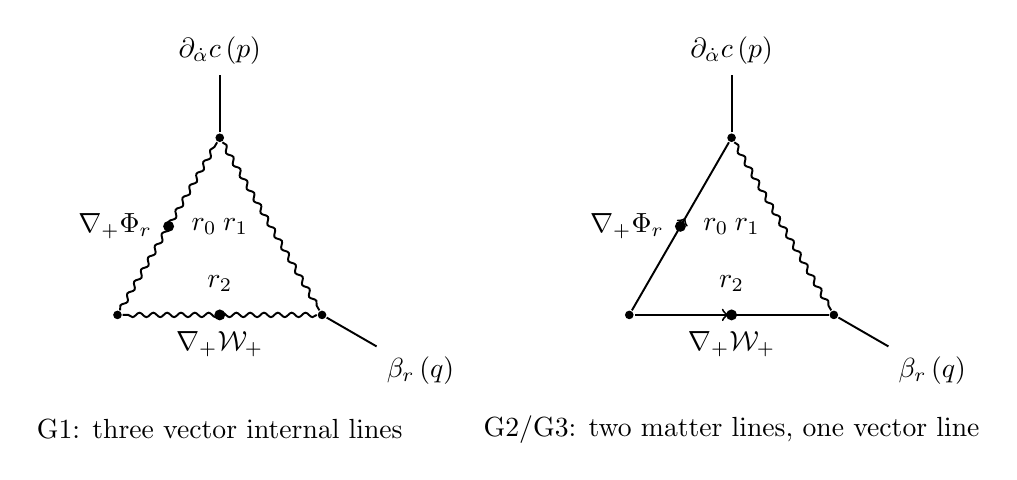
\begin{tikzpicture}[baseline]
\node[svertex] (v0) at (90:1.5) {}; \node[svertex] (v1) at (210:1.5) {}; \node[svertex] (v2) at (330:1.5) {};
\draw[sV] (v1) -- node[midway,sinsert,label=left:{$\nabla_{+}\Phi_{r}$}] {} (v0); \draw[sV] (v0) -- (v2);
\draw[sV] (v2) -- node[midway,sinsert,label=below:{$\nabla_{+}\cW_{+}$}] {} (v1);
\draw[sleg] (v0) -- ++(90:0.8) node[above] {$\partial_{\dot\alpha}c\,(p)$};
\draw[sleg] (v2) -- ++(330:0.8) node[anchor=north west] {$\beta_{r}\,(q)$};
\node at ($(v1)!0.5!(v0)+(0.45,0)$) {$r_{0}$}; \node at ($(v0)!0.5!(v2)+(-0.45,0)$) {$r_{1}$}; \node at ($(v2)!0.5!(v1)+(0,0.4)$) {$r_{2}$};
\node at (0,-2.2) {G1: three vector internal lines};
\begin{scope}[xshift=6.5cm]
\node[svertex] (w0) at (90:1.5) {}; \node[svertex] (w1) at (210:1.5) {}; \node[svertex] (w2) at (330:1.5) {};
\draw[sPhi] (w1) -- node[midway,sinsert,label=left:{$\nabla_{+}\Phi_{r}$}] {} (w0); \draw[sV] (w0) -- (w2);
\draw[sPhit] (w2) -- node[midway,sinsert,label=below:{$\nabla_{+}\cW_{+}$}] {} (w1);
\draw[sleg] (w0) -- ++(90:0.8) node[above] {$\partial_{\dot\alpha}c\,(p)$};
\draw[sleg] (w2) -- ++(330:0.8) node[anchor=north west] {$\beta_{r}\,(q)$};
\node at ($(w1)!0.5!(w0)+(0.45,0)$) {$r_{0}$}; \node at ($(w0)!0.5!(w2)+(-0.45,0)$) {$r_{1}$}; \node at ($(w2)!0.5!(w1)+(0,0.4)$) {$r_{2}$};
\node at (0,-2.2) {G2/G3: two matter lines, one vector line};
\end{scope}
\end{tikzpicture}
\caption{The ordered triangles of the $(b,\beta_r)/(\beta_r,b)$ family in the routing~\eqref{eq:ss:ab:routing}: one $\nabla_+\cW_+$ and one $\nabla_+\Phi_r$ insertion (filled dots), residual external legs $\partial c(p)$, $\beta_r(q)$. The right panel shows the G2 line content (vector edge $r_1$, legs $\partial c,\beta_r$); the two G3 routings share the vertex structure with the vector edge on $r_0$ and the antichiral legs $\gamma^s,\gamma^t$ in place of $\partial c,\beta_r$, one matter-cubic vertex replaced by the antichiral superpotential vertex.}
\label{fig:ss:ab:triangles}
\end{figure}
Excluded from the graph sum: the zero-square current bubbles $JE,JX,PE,PX$, which cancel in exact pairs ($I_{JE}+I_{JX}=0$, $I_{PE}+I_{PX}=0$) and contain no four-dimensional inverse square, so each DRED defect is zero; and the separately drawn source-resolvent bubbles, which are presentations of the same induced derivative-of-action contact and are not independent anomaly graphs.

\paragraph{2. Wick contractions.} The Euclidean propagators in the canonically normalized frames are
\begin{equation}\label{eq:ss:ab:propagators}
\langle\cV^{A}(p,1)\cV^{B}(-p,2)\rangle_E
=-\frac{2\h g^{2}\kappa^{AB}}{p^{2}}\,\delta^{4}(\theta_{12}),
\qquad
\langle\Phi_r^{A}(p,1)\widetilde\Phi^{sB}(-p,2)\rangle_E
=\delta_r{}^{s}\,\frac{\h g^{2}\kappa^{AB}}{16\,p^{2}}\,
\bcD_1^{2}\cD_1^{2}\,\delta^{4}(\theta_{12}) .
\end{equation}
For G3 the flavor- and chirality-preserving Wick pairing is unique: the vector legs of the source and matter vertices pair along $r_0$, the matter leg of the matter vertex pairs with an antichiral leg of the superpotential vertex along $r_1$, and the source matter leg pairs with the remaining antichiral leg along $r_2$; the two uncontracted legs are the external legs. There is no second preserving pairing and no graph automorphism division, so
\begin{equation}\label{eq:ss:ab:cprop}
C_{\mathrm{prop}}=(-\h)\left(\frac{\h}{16}\right)^{2}=-\frac{\h^{3}}{256} .
\end{equation}
Every primitive weight is one:
\begin{equation}\label{eq:ss:ab:mult}
\left[\tfrac12(2)_{\text{cyc.\ source}}\right]
\left[\tfrac1{2!}(2)_{\text{vertex orders}}\right]
\left[\tfrac1{3!}(6)_{\text{gauge-vertex labels}}\right]
\left[\tfrac1{3!}(6)_{\cV\Phi\widetilde\Phi}\right]
(1)_{\mathrm{Wick}}=1\ \text{(G1)},\qquad
\left[\tfrac12(2)\right]
\left[\tfrac1{2!}(2)\right]
\left[\tfrac1{3!}(6)_{\text{superpotential labels}}\right]
(1)_{\mathrm{Wick}}=1\ \text{(G3)} .
\end{equation}

\paragraph{3. Amplitude assembly.} The mixed source Hessian, the matter-cubic vertex, and the antichiral superpotential vertex (from $W$ of Section~\ref{sec:notation}) contribute, with~\eqref{eq:ss:ab:cprop} and the unit factorial weights~\eqref{eq:ss:ab:mult},
\begin{equation}\label{eq:ss:ab:vertexconstants}
C_I=-\frac{g^{2}}{4\sqrt2},
\qquad
C_M=\frac{\sqrt2\,g}{\h},
\qquad
C_{H_-}=-\frac{\sqrt2\,g}{\h};
\qquad
C_{\mathrm{preD}}^{G2}=C_I C_M^{2}C_{\mathrm{prop}}=+\frac{\sqrt2\,\h g^{4}}{1024},
\qquad
C_{\mathrm{preD}}^{32}=C_I C_M C_{H_-}C_{\mathrm{prop}}=-\frac{\sqrt2\,\h g^{4}}{1024},
\qquad
C_{\mathrm{preD}}^{33}=+\frac{\sqrt2\,\h g^{4}}{1024},
\end{equation}
the relative sign of $G_{3,2},G_{3,3}$ being the ordered flavor/color reflection sign of the superpotential vertex. The residual external-leg operators are: for G1, the pairing $X_{\partial c\,\beta}:=\langle\partial c,\beta_r\rangle$ and the equation-of-motion composite $E:=\beta_r\,(P^{\dot\alpha}\partial_{\dot\alpha}c)$ ($P^{\dot\alpha}$ the holomorphic momentum of the $\partial c$ leg in Fourier space); for G2, the single word $\tfrac13\,\beta_r(4p-q)^{\dot\alpha}\partial_{\dot\alpha}c$; for G3, the uncontracted $\gamma^s,\gamma^t$ legs, contracted by the wedge $W_{ij}:=r_{i,+}\wedge r_{j,+}=r_{i,+\dot\alpha}r_{j,+}{}^{\dot\alpha}$, $W_{ji}=-W_{ij}$.

\paragraph{4. The $D$-algebra chain.} Discarding a longitudinal word at edge $e$ against the neighboring projector at edge $n$ transports the occurrence by superspace integration by parts; the endpoint sign, the corner identity, and the loop-saturation $16$ give the universal transport factor and its full-$d$ companion
\begin{equation}\label{eq:ss:ab:transport}
\left(-\frac12\right)(-1)(16)=8,
\qquad
8\,\bar r_n^{\,2}\,\mathcal T_{e|n}-8\,r_{n,d}^{\,2}\,\mathcal T_{e|n}
=8\,\mul^{2}\,\mathcal T_{e|n} .
\end{equation}
For G3 the raw Grassmann-measure monomial, converted to the full measure, settles the unit
\begin{equation}\label{eq:ss:ab:unit4096}
32768\left(\tfrac14\right)_{d^{4}\theta_M}
\left(\tfrac12\right)_{d^{2}\bar\theta_H}
\left(-\tfrac12\right)_{\mul^{2}\text{ extraction}}
(2)_{\text{trace/metric}}=-4096 ,
\end{equation}
the trace/metric factor $2$ being algebraic and canceled by the $-\tfrac12$ rank extraction, not a graph multiplicity. The three kinetic cuts and their parents are, with $W_0=W_{12}$, $W_1=W_{P0}$, $W_2=W_{p0}$,
\begin{align}
K_0&=+4096\,W_0,
&
K_1&=-4096\,W_1,
&
K_2&=+4096\,W_2,
\label{eq:ss:ab:cuts}\\
P_0&=-4096\,(D_0+\mul^{2})\,W_0,
&
P_1&=+4096\,(D_1+\mul^{2})\,W_1,
&
P_2&=-4096\,(D_2+\mul^{2})\,W_2 .
\label{eq:ss:ab:parents}
\end{align}
For G2 the selected and transported occurrences give
\begin{equation}\label{eq:ss:ab:g2pair}
-\frac{8\,(D_2+\mul^{2})\,\mathcal R}{D_0D_1D_2}
+\frac{8\,\mathcal R}{D_0D_1}
=-\frac{8\,\mul^{2}\,\mathcal R}{D_0D_1D_2},
\qquad
-\tfrac12\,(D_1+\mul^{2})\,W+\tfrac12\,D_1W=-\tfrac12\,\mul^{2}W ,
\end{equation}
and every G1 row obeys $F_A+C_{A,d}=-8R_A\,\mul^{2}$, $F_B+C_{B,d}=-8R_B\,\mul^{2}$, with $C_{A,d}=-L_A-\alpha_A r_{2,d}^{2}$, $\alpha_A=-8R_A$, $L_A=-\tfrac12\cD_+\bcD^{2}\cD^{2}$. The wedge algebra of the three G3 remainders closes pointwise: with $r_1=r_0-p$, $r_2=r_0-p-q$,
\begin{equation}\label{eq:ss:ab:wedge}
-W_{12}+W_{P0}-W_{p0}=-\,p_+\wedge q_+
\quad\Longrightarrow\quad
\mathcal R_{G3}^{\mathrm{full}}
=-\frac{4096\,\mul^{2}\,(p_+\wedge q_+)}{D_0D_1D_2} .
\end{equation}

\paragraph{5. Evanescent extraction and the rank-one moments.} Every remainder of step 4 is governed by the cutting-failure identity~\eqref{eq:ss:cuttingfailure} and the master integral~\eqref{eq:ss:masterintegral}. The rank-one moments are the ordered-simplex averages
\begin{equation}\label{eq:ss:ab:moments}
\lim_{\epsilon\to0}\int_{\ell}\frac{\mul^{2}\,\bar r_0^{\mu}}{D_0D_1D_2}
=\frac{2p^{\mu}+q^{\mu}}{96\pi^{2}},
\qquad
\lim_{\epsilon\to0}\int_{\ell}\frac{\mul^{2}\,\bar r_1^{\mu}}{D_0D_1D_2}
=\frac{q^{\mu}-p^{\mu}}{96\pi^{2}},
\qquad
\lim_{\epsilon\to0}\int_{\ell}\frac{\mul^{2}\,\bar r_2^{\mu}}{D_0D_1D_2}
=-\frac{p^{\mu}+2q^{\mu}}{96\pi^{2}},
\qquad
\lim_{\epsilon\to0}\int_{\ell}\frac{\mul^{2}\,W_{p0}}{D_0D_1D_2}
=\frac{W(p,q)}{96\pi^{2}},
\end{equation}
from $2\int_{\Sigma_2}x_i\,dx_1dx_2=\tfrac13$ per coordinate. Applied graph by graph: G1 integrates to the mark coefficients $(\tfrac43,\tfrac23)$, $(\tfrac23,\tfrac43)$ in the two slot orderings, i.e.\ the word $2(p+q)^{\dot\alpha}\beta_r\,\partial_{\dot\alpha}c=2\,P^{\dot\alpha}\bigl(\beta_r\,\partial_{\dot\alpha}c\bigr)$, a pure total derivative vanishing in the quotient; G2 integrates to the selected word $\tfrac23\,\beta_r(2p+q)^{\dot\alpha}\partial_{\dot\alpha}c$ plus the transported word $-\beta_r\,q^{\dot\alpha}\partial_{\dot\alpha}c$, i.e.\ $\tfrac13\,\beta_r(4p-q)^{\dot\alpha}\partial_{\dot\alpha}c$ with pair/equation-of-motion coefficients $(-\tfrac13,\tfrac43)$ on the graph-word placement (Remark~\ref{rem:ss:ab:slotmap}); G3 carries the marked simplex weights $\tfrac23,\tfrac13$ per mark and sums to the raw wedge coefficients $+2\sqrt2\,i$ ($G_{3,2}$) and $-2\sqrt2\,i$ ($G_{3,3}$) in units of $\h g^{2}/(16\pi^{2})$. Passing from the raw momentum wedge to the dotted bilinear flips the sign once, since with the locked phase $e^{ipx}$, $(ip)_+\wedge(iq)_+=-(p_+\wedge q_+)$.

\paragraph{6. Pole cancellation.} No $1/\epsilon$ pole occurs anywhere in this family: every parent-plus-contact pair vanishes identically at $\mul^{2}=0$,
\begin{align}
\frac{P_0}{D_0D_1D_2}+\frac{K_0}{D_1D_2}
&=-\frac{4096\,\mul^{2}W_0}{D_0D_1D_2},
&
\frac{P_1}{D_0D_1D_2}+\frac{K_1}{D_0D_2}
&=+\frac{4096\,\mul^{2}W_1}{D_0D_1D_2},
&
\frac{P_2}{D_0D_1D_2}+\frac{K_2}{D_0D_1}
&=-\frac{4096\,\mul^{2}W_2}{D_0D_1D_2},
\label{eq:ss:ab:polecancel}
\end{align}
and likewise for the G2 pairs~\eqref{eq:ss:ab:g2pair} and the G1 rows. Only the evanescent remainders survive. (Contrast the seed channel $(b,b)$, where literal $1/\epsilon$ poles cancel between the parent triangle and the Schwinger contact rows.)

\paragraph{7. Raw carrier, total-derivative quotient, finite shift.} Collect the integrated outputs as coefficient vectors of unit-normalized carriers in the ordered basis of candidate bilinears
\begin{equation}\label{eq:ss:ab:basis}
\bigl(X_{\partial c\,\beta},\,E,\,X_{\beta\,\partial c},\,E,\,
C_{st},\,C_{ts}\bigr),
\qquad
X_{\beta\,\partial c}:=\langle\beta_r,\partial c\rangle,
\quad
C_{st}:=\langle\gamma^{s},\gamma^{t}\rangle,
\quad
C_{ts}:=\langle\gamma^{t},\gamma^{s}\rangle,
\end{equation}
with $\varepsilon_{rst}=+1$ and $E:=\beta_r\bigl(P^{\dot\alpha}\partial_{\dot\alpha}c\bigr)$ the equation-of-motion composite of step 3, entering in both orderings. The two pairings are a single carrier: the odd--odd Koszul swap ($|\partial c|=|\beta_r|=1$) and the dotted-index flip $\psi^{\dot\alpha}\chi_{\dot\alpha}=-\psi_{\dot\alpha}\chi^{\dot\alpha}$ of the locked convention cancel,
\begin{equation}\label{eq:ss:ab:paireq}
X_{\partial c\,\beta}=(\partial_{\dot\alpha}c)(\partial^{\dot\alpha}\beta_r)
=-(\partial^{\dot\alpha}\beta_r)(\partial_{\dot\alpha}c)
=(\partial_{\dot\alpha}\beta_r)(\partial^{\dot\alpha}c)
=X_{\beta\,\partial c}=:X .
\end{equation}
There is accordingly one total-derivative identity, not two: the even derivation $P^{\dot\alpha}$ acting on the odd--odd product gives no Koszul sign, and the pair term enters with the index flip $(P^{\dot\alpha}\beta_r)\partial_{\dot\alpha}c=-\langle\beta_r,\partial c\rangle=-X$,
\begin{equation}\label{eq:ss:ab:td}
T:=P^{\dot\alpha}\bigl(\beta_r\,\partial_{\dot\alpha}c\bigr)
=\bigl(P^{\dot\alpha}\beta_r\bigr)\partial_{\dot\alpha}c
+\beta_r\bigl(P^{\dot\alpha}\partial_{\dot\alpha}c\bigr)
=-X+E ,
\end{equation}
so $aX+bE=(a+b)X+bT$ in either ordering. (Equivalently $P^{\dot\alpha}(\partial_{\dot\alpha}c\,\beta_r)=X-E=-T$: a single ray. The combination $X+E$ is not a total derivative, and $X$ itself is not one either.) The raw pair coefficients displayed below are quoted on the graph-word placement $X_{>}:=(\partial^{\dot\alpha}\beta_r)\partial_{\dot\alpha}c=-X$, where the same identity reads $T=X_{>}+E$, i.e.\ $aX_{>}+bE=(a-b)X_{>}+bT$: thus the G1 entries $(2,2)_{(X_{>},E)}=(0,2)_{(X_{>},T)}$ quotient to zero, and the G2 split and quotient are the machine-sealed replay values of Remark~\ref{rem:ss:ab:slotmap}. The coefficient flow of the family is the aligned display
\begin{align}
\text{raw graph carrier:}\quad
&\bigl(2,\;2,\;-\tfrac13,\;\tfrac43,\;-2i\sqrt2,\;+2i\sqrt2\bigr)
\quad\text{on the six-carrier basis }\eqref{eq:ss:ab:basis},
\label{eq:ss:ab:flowraw}\\[2pt]
\text{total-derivative quotient:}\quad
&\bigl(0,\;1,\;-2i\sqrt2,\;+2i\sqrt2\bigr)
\quad\text{on }
\bigl(X_{\partial c\,\beta},X_{\beta\,\partial c},C_{st},C_{ts}\bigr),
\label{eq:ss:ab:flowtd}\\[2pt]
\text{finite normal-product shift:}\quad
&+\;\bigl(1,\;0,\;+i\sqrt2,\;-i\sqrt2\bigr),
\label{eq:ss:ab:flowshift}\\[2pt]
\text{renormalized vector:}\quad
&\bigl(1,\;1,\;-i\sqrt2,\;+i\sqrt2\bigr) .
\label{eq:ss:ab:flowren}
\end{align}
The shift is fixed by residual supersymmetry: acting with the $q_r$ of~\eqref{eq:ss:qaction} (stated with the channel table in Section~\ref{sec:superspace:table}) on a general vector $x=(x_1,x_2,x_3,x_4)$ in the four-component basis, the Ward conditions of the descendant system $q_s[\,x\cdot(\text{basis})\,]=i\delta_{sr}\,\Delta(b,b)$ of~\eqref{eq:ss:triplet} --- the homogeneous $s=2,3$ mixing plus the $s=1$ matching against the anchored $(b,b)$ singlet, restricted to this flavor ansatz --- read
\begin{equation}\label{eq:ss:ab:ward}
x_1-x_2=0,
\qquad
i\sqrt2\,x_1+x_3=0,
\qquad
-i\sqrt2\,x_1+x_4=0 ,
\end{equation}
a rank-three system whose solution space is the ray $x=t\,(1,1,-i\sqrt2,+i\sqrt2)$: the renormalized vector~\eqref{eq:ss:ab:flowren} is exactly annihilated by~\eqref{eq:ss:ab:ward}, and the descendant identity~\eqref{eq:ss:triplet} anchors the ray to the $(b,b)$ scale, fixing $t=1$.

\begin{remark}[The finite shift is a scheme term, not a new anomaly graph]%
\label{rem:ss:ab:shift}
The vector~\eqref{eq:ss:ab:flowshift} is a finite composite-source normal-product (scheme) term. It is not a triangle, collapsed graph, Schwinger cut, inverse-square occurrence, or new cutting failure: all bare-graph anomaly of this family enters through the $\mul^{2}$ remainders of steps 4--6, and the shift is precisely what removes the residual factor of two between the raw G3 $\gamma\gamma$ coefficients and the Ward-compatible ray.
\end{remark}

\begin{remark}[Granularity of the machine replays]\label{rem:ss:ab:machine}
Three ingredients are sealed at machine level and displayed here at the granularity of the extracted formulas: the full 192-row G1 $D$-word table (only test-point rows admit an analytic display; the row identities $F_A+C_{A,d}=-8R_A\mul^{2}$, $F_B+C_{B,d}=-8R_B\mul^{2}$ hold for every row), the replay producing the G2 raw residual, and the color-route phase $+i$ of the G3 coefficients. All quoted coefficients are the machine-checked ones.
\end{remark}

\begin{remark}[Placement sensitivity of the G2 slot map]\label{rem:ss:ab:slotmap}
The decomposition of the G2 word $\tfrac13\beta_r(4p-q)^{\dot\alpha}\partial_{\dot\alpha}c$ is placement-sensitive: on the graph-word placement $(\partial^{\dot\alpha}\beta_r)\partial_{\dot\alpha}c$ the pair coefficient is $-\tfrac13$, while on the canonical pairing $\langle\beta_r,\partial c\rangle=-(\partial^{\dot\alpha}\beta_r)\partial_{\dot\alpha}c$ of~\eqref{eq:ss:ab:paireq} it is $+\tfrac13$, and the consistent md-level total-derivative quotient of the displayed word on the canonical carrier is $\tfrac53$. The intermediate slot-map displays mix the two placements (the typed slot map of the Omega-routing audit versus the identity $(P^{\dot a}B_1)D_{\dot a}=-\langle B_1,D\rangle$ of the external-divergence audit). The displayed G2 raw pair/EOM entries and the quotient value $+1$ in~\eqref{eq:ss:ab:flowtd} are therefore machine-sealed by the typed replay rather than derived at md level. The renormalized endpoint does not depend on this link: the Ward ray and its unit scale are anchored by the descendant identity~\eqref{eq:ss:triplet}, and the full renormalized vector matches the holomorphic-twist target word by word in the 81/81 machine round-trip.
\end{remark}

\paragraph{8. The final result.} Restoring the letter normalizations~\eqref{eq:ss:letters} --- the insertions contribute $(-i/\sqrt2)(1/\sqrt2)=-i/2$, each dotted output pair contributes $-i\sqrt2$, and the $\gamma$ pairs contribute $1$, so the unit-normalized vector is $-i\sqrt2$ times the bracket and $(-i/2)(-i\sqrt2)=-1/\sqrt2$ --- the renormalized vector~\eqref{eq:ss:ab:flowren} becomes the channel-table row
\begin{equation}\label{eq:ss:ab:result}
\boxed{\;
\nabla_{-}\big(b^{A}\beta_r^{B}\big),\quad
\nabla_{-}\big(\beta_r^{A}b^{B}\big)
=-\frac{\h g^{2}}{16\sqrt2\,\pi^{2}}\,f^{ACD}f^{BCE}\,
\big\{\langle\beta_{r},\partial c\rangle
+\langle\partial c,\beta_{r}\rangle
+\varepsilon_{rst}\langle\gamma^{s},\gamma^{t}\rangle\big\}^{DE} ,\;}
\end{equation}
in exact agreement with~\eqref{eq:ss:ch-bbeta}. The two orderings are equal: the source-order Koszul sign is $(-1)^{|b||\beta|}=(-1)^{0\cdot1}=+1$, the superpotential flavor/color reflection contributes $+1$, the simplex moments are invariant under the reflection relabeling, and the reflected vector maps word by word onto~\eqref{eq:ss:ab:flowren}.

\paragraph{9. Comparison with the holomorphic twist.} Budzik and Kulp print, for this family, \cite[eq.~(3.68)]{BK}
\begin{equation}\label{eq:ss:ab:bk}
Q_1\big((\beta_I)^{A}b^{B}\big)
=\kappa^{2}f_{ACD}f_{BCE}
\Big[\partial_{\dot\alpha}(\beta_I)^{D}\partial^{\dot\alpha}c^{E}
+\partial_{\dot\alpha}c^{D}\partial^{\dot\alpha}(\beta_I)^{E}
+\varepsilon_{IJK}\,\partial_{\dot\alpha}(\gamma^{J})^{D}
\partial^{\dot\alpha}(\gamma^{K})^{E}\Big] .
\end{equation}
Under the letter dictionary of Section~\ref{sec:ht}, the three words of~\eqref{eq:ss:ab:bk} map exactly onto $\langle\beta_r,\partial c\rangle+\langle\partial c,\beta_r\rangle$ and $\varepsilon_{rst}\langle\gamma^{s},\gamma^{t}\rangle$, and BK's prefactor $\kappa^{2}$ maps onto $-\h g^{2}/(16\sqrt2\,\pi^{2})$: the match is word by word, for both orderings. The reversed ordering $Q_1(b^{A}(\beta_I)^{B})$ is not printed as a final display in \cite{BK}; it is fixed there by the descent relations, and the machine round-trip confirms the identical canonical word for both directions. Two source inconsistencies of \cite{BK} are recorded in Section~\ref{sec:ht}: the missing $\Gamma(3)=2$ in their printed triangle kernel, and the $-\tfrac14$ versus $-\kappa^{2}$ clash, adjudicated to the main branch $-\kappa^{2}$.

\begin{remark}[Status of the comparison]\label{rem:ss:ab:htstatus}
The match with~\eqref{eq:ss:ab:bk} is a cross-check against an external target, not a completeness proof of the graph census: the adversarial seventeen-candidate census review remains open, and no holomorphic-twist coefficient enters the derivation of~\eqref{eq:ss:ab:result}. Before the finite shift~\eqref{eq:ss:ab:flowshift}, the raw $G_{3,2},G_{3,3}$ coefficients are exactly twice their twist counterparts in every common basis (since $\varepsilon_{1JK}X_{JK}=X_{23}-X_{32}$); the shift is what removes this factor two.
\end{remark}

\subsection{The channels $(b,\gamma^{r})$ and $(\gamma^{r},b)$}%
\label{sec:superspace:bgamma}

We now compute the mixed vector--antichiral family: the six ordered channels $(b,\gamma^{r})$ and $(\gamma^{r},b)$,
$r=1,2,3$, of the master identity~\eqref{eq:ss:master}. The two ordered insertions are
\begin{equation}\label{eq:bg:insert}
I_{b\gamma^{r}}=\nabla_{-}\big(b^{A}\gamma^{rB}\big), \qquad I_{\gamma^{r}b}=\nabla_{-}\big(\gamma^{rA}b^{B}\big) .
\end{equation}
Both letters are Grassmann-even and $\nabla_{-}\gamma^{r}=0$, so in each insertion the outer derivative marks only
the $b$ line; every nonlinear occurrence of the covariantized source is nevertheless retained. The two directions
are computed independently below --- no graph coefficient is copied from one ordering to the other. As in the seed
channel, the graph weights are assembled with the unit-normalized field-strength insertion $X:=\nabla_{+}\cW_{+}$;
the letter normalization $b=-(i/\sqrt2)X$ is restored only in the final step.

\paragraph{1. Graph inventory.} The covariant completion of the insertion and its $\cD_{-}$-words are
\begin{equation}\label{eq:bg:source}
X_{c}=X_{1}+gX_{2}+g^{2}X_{3}, \qquad N_{0}=\cD_{-}X_{1}, \quad N_{1}=\cD_{-}X_{2}+[\Gamma_{1},X_{1}], \quad N_{2}=\cD_{-}X_{3}+[\Gamma_{1},X_{2}]+[\Gamma_{2},X_{1}],
\end{equation}
where $\nabla_{-}=\cD_{-}+g\Gamma_{1}+g^{2}\Gamma_{2}$ is the connection expansion of the semi-chiral derivative,
while $\gamma^{r}=\widetilde\Phi^{r}$ has no nonlinear completion. The connected order-$g^{2}$ orbit is
\begin{equation}\label{eq:bg:orbit}
\Gamma^{(1)}_{g^{2}} =\langle I_{2}\rangle_{0} -\frac1\h\langle I_{1}S_{3}\rangle_{0,c} -\frac1\h\langle I_{0}S_{4}\rangle_{0,c} +\frac1{2\h^{2}}\langle I_{0}S_{3}S_{3}\rangle_{0,c} ,
\end{equation}
with $I_{n}$ the source term at order $g^{n}$, $S_{3}$ and $S_{4}$ the cubic and quartic action vertices, and
$\langle\;\rangle_{0,c}$ the connected Gaussian average. The admitted parent triangle skeletons are the
gauge--matter class $T_{GM}^{(r)}=(I,G,M_{r})$ and the two-matter class $T_{MM}^{(r,r)}=(I,M_{r},M_{r})$, with
$G=\mathcal V_{VVV}$ the cubic gauge vertex and $M_{r}=\mathcal V_{\widetilde\Phi_{r}V\Phi_{r}}$ the matter--gauge
cubic; the superpotential class $T_{MH}=(I,M_{r},H_{\widetilde\Phi^{3}})$ contributes two complement-flavor routes
per direction, both exactly zero by
\eqref{eq:bg:tmh} below, and there is no all-gauge parent for this letter pair. Per ordered direction the route census is
\begin{equation}\label{eq:bg:census}
N_{TGM}=6, \qquad N_{TMM}=1, \qquad N_{TMH}=2 ,
\end{equation}
the six gauge--matter routes being the six permutations of the three internal edges $(r_{0},r_{1},r_{2})$, each
with two derivative placements times two Euclidean chiralities of the matter line. Figure~\ref{fig:bg:triangle}
shows the ordered triangle in the two-matter topology.

\begin{figure}[t]
\centering
\begin{tikzpicture}[scale=1.15]
  \coordinate (I)  at (90:2.0);
  \coordinate (ML) at (210:2.0);
  \coordinate (MR) at (330:2.0);
  \draw[sV]    (I)  -- (ML) node[midway,left=3pt]  {$r_{0}$};
  \draw[sPhi]  (ML) -- (MR) node[midway,below=3pt] {$r_{1}$};
  \draw[sPhit] (MR) -- (I)  node[midway,right=3pt] {$r_{2}$};
  \draw[sPhit] (ML) -- ++(180:1.5) node[left]  {$\widetilde\Phi^{r}\ (p)$};
  \draw[sleg] (MR) -- ++(0:1.5)   node[right] {$\partial_{\dot\alpha}c\ (q)$};
  \node[sinsert,label={90:$\nabla_{-}\bigl(b^{A}\gamma^{rB}\bigr)$}] at (I) {};
  \node[svertex,label=below left:{$M_{r}$}]  at (ML) {};
  \node[svertex,label=below right:{$M_{r}$}] at (MR) {};
\end{tikzpicture}
\caption{The ordered triangle of the $(b,\gamma^{r})$ family in the two-matter topology $T_{MM}^{(r,r)}$. The filled
insertion node carries the letter operator $\nabla_{-}(b^{A}\gamma^{rB})$ with $b=-(i/\sqrt2)\nabla_{+}\cW_{+}$;
the internal edges are the source-$b$ vector line $r_{0}$ (wavy), the chiral matter bridge $r_{1}$, and the
source-$\gamma$ reversed-chiral line $r_{2}$, with $r_{1}-r_{0}=p$. The external antichiral letter
$\gamma^{r}=\widetilde\Phi^{r}$ (momentum $p$) enters at the left matter vertex, the vertex where the vector
edge $r_{0}$ attaches (each matter cubic vertex has exactly one vector slot); the vector output letter
$\partial_{\dot\alpha}c$ (momentum $q$) enters at the right matter vertex. The gauge--matter topology
$T_{GM}^{(r)}$ replaces the left matter vertex by the cubic gauge vertex $G$ (the edges incident to $G$ are
vector lines); its six ordered routings of $(r_{0},r_{1},r_{2})$ are the six permutation routes of the text, and
the reversed channel $(\gamma^{r},b)$ has the same figure with the source attachments exchanged.}
\label{fig:bg:triangle}
\end{figure}

\paragraph{2. Wick contractions.} Every labeled Wick contraction carries weight $1$: the $1/2!$ of the two cubic action
copies is canceled by the two labeled action orderings,
\begin{equation}\label{eq:bg:wick}
w_{\mathrm{Wick}}=\frac{1}{2!}\,(1+1)=1 ,
\end{equation}
and no residual symmetry factor occurs anywhere in the family. In the triangle term $\langle
I_{0}S_{3}S_{3}\rangle_{0,c}$ the two external ports attach to two distinct cubic vertices and the three internal
edges are paired among the vertex slots, giving the six $T_{GM}$ routings, the single $T_{MM}$ routing (two matter
propagators, hence two chiral projectors), and the two $T_{MH}$ routings. In the nonlinear-source bubble $\langle
I_{1}S_{3}\rangle_{0,c}$ the two internal legs of the connection word $[\Gamma_{1},X_{1}]$ pair with each other
through the loop, and the cubic matter vertex ties the loop to the external $\gamma^{r}$ leg. The quartic seagull
$\langle I_{0}S_{4}\rangle_{0,c}$ is a single graph: differentiating
\begin{equation}\label{eq:bg:seagull}
[\cV,[\cV,\Phi]]=\cV^{2}\Phi-2\cV\Phi\cV+\Phi\cV^{2}
\end{equation}
with respect to one internal and one external $\cV$ places both orderings inside one seagull vertex; they are not
two Feynman graphs. The remaining source tadpole $\langle I_{2}\rangle_{0}$ is a single coincident vector loop. The
full color contraction of the family --- two matter vertices, two matter inverse metrics, and the complete vector
covariance --- reduces, with $[T_{A},T_{B}]=if_{AB}{}^{C}T_{C}$ and $\operatorname{tr}(T_{A}T_{B})=\delta_{AB}/2$,
to
\begin{equation}\label{eq:bg:color}
C_{\mathrm{full}} \;\propto\; \sum_{X}\operatorname{tr}\big(T_{D}[T_{A},T_{X}]\big) \operatorname{tr}\big(T_{X}[T_{E},T_{B}]\big) \;\longrightarrow\; +\,f^{ACD}f^{BCE} ,
\end{equation}
the numerical proportionality being carried into the assembled prefactors of paragraph 3. This is the adjudicated
signed color word of the family: the same tensor unit as in the master identity~\eqref{eq:ss:master}.

\paragraph{3. Amplitude assembly.} The propagators entering the orbit are the vector line and the two matter
orientations,
\begin{equation}\label{eq:bg:props}
-\frac{\h}{\BoxE}, \qquad +\frac{\h\,\bcD^{2}\cD^{2}}{16\,\BoxE}, \qquad +\frac{\h\,\cD^{2}\bcD^{2}}{16\,\BoxE} ;
\end{equation}
each matter vertex contributes $+\sqrt2\,g/\h$ with measure $1/4$ per vertex, and the canonical source
normalization is $-1/(4\sqrt2)$. The two-matter orbit therefore assembles to the exact pre-$D$ factor
\begin{equation}\label{eq:bg:tmmpre}
\left(-\frac{1}{4\sqrt2}\right)\left(\frac{\sqrt2\,g}{\h}\right)^{2} \left[-\h\left(\frac{\h}{16}\right)^{2}\right]=\frac{\sqrt2\,\h g^{2}}{1024} ,
\end{equation}
while each gauge--matter route carries, per Euclidean chirality,
\begin{equation}\label{eq:bg:tmpre}
\mathrm{preD}_{-}=+\frac{\h g^{2}}{8192\sqrt2}, \qquad \mathrm{preD}_{+}=-\frac{\h g^{2}}{8192\sqrt2} .
\end{equation}
After loop saturation the external legs carry residual operator words: the $\gamma^{r}$ leg is a plain antichiral
field (factor $1$), and the vector output leg collapses as
\begin{equation}\label{eq:bg:residual}
\cD^{2}\bcD_{\dot\alpha}\,u=-4\sqrt2\,D_{\dot\alpha}, \qquad \cD^{2}\bcD_{\dot\alpha}\,(\theta+\bar\theta\,\theta_{\dot\alpha})=-2 ,
\end{equation}
where $u$ is the formal leg slot and $D_{\dot\alpha}$ the unit vector output slot (the antichiral field strength
$\bcW_{\dot\alpha}$; the letter $\partial_{\dot\alpha}c=i\bcW_{\dot\alpha}$ is restored in paragraph 7). The
ordered output kernels are $(\partial_{\dot\alpha}Y)^{D}D^{E\dot\alpha}$ for the two-matter orbit and
$D_{\dot\alpha}^{D}(\partial^{\dot\alpha}Y)^{E}$ for the gauge--matter orbit, with $Y=\widetilde\Phi^{r}$.

\paragraph{4. The $D$-algebra chain.} The master $D$-word behind every route is
\begin{equation}\label{eq:bg:masterD}
\cD_{-}\cD_{+}\bcD^{2}\cD_{+} =8\,\bar\Box\,\cD_{+}-\frac12\,\cD_{+}\bcD^{2}\cD^{2} ,
\end{equation}
with $\bar\Box$ the d'Alembertian of the barred spin metric of \eqref{eq:ss:sigmaalgebra}; loop saturation uses
$\delta^{4}(\theta_{12})\cD^{2}\bcD^{2}\delta^{4}(\theta_{12})=16\,\delta^{4}(\theta_{12})$ as in the seed channel.
For the two-matter route the four-dimensional numerator before the metric split is
\begin{equation}\label{eq:bg:tmmnum}
\mathcal F^{(4)}_{b>\gamma} =8(\det r_{0})\,\mathcal R_{0}-8(\det r_{1})\,\mathcal J_{1}, \qquad \mathcal R_{0}=-128\,\mathfrak b(r_{1}), \qquad \mathcal J_{1}=-128\,\mathfrak b(r_{0}) ,
\end{equation}
where $r_{0}$ is the source-$b$ vector edge, $r_{1}$ the chiral bridge, $\det r_{e}$ the $2\times2$ determinant of
the edge momentum (kept symbolic; its index-level definition is not needed below), and $\mathfrak b(\cdot)$ the
external bilinear carrier. The collapsed neighbor of the same cut orbit, its migrated and transverse residuals, and
the projector-collapse check are
\begin{equation}\label{eq:bg:tmmcontact}
K_{\mathrm{neighbor}}=(64\,r_{0\dot2},\,-64\,r_{0\dot1}), \quad (-128\,r_{0\dot2},\,+128\,r_{0\dot1}), \quad \big(+128(p_{\dot2}-r_{0\dot2}),\,-128(p_{\dot1}-r_{0\dot1})\big), \quad 16\det(r_{1})\,K_{\mathrm{neighbor}}=-8\det(r_{1})\,\mathcal J_{1} ,
\end{equation}
with the longitudinal tag migrating the source vector $r_{0}$ into the adjacent chiral projector $r_{1}$; for the
reversed direction the inverse-edge rows read $+8\det(r_{2})\mathcal R_{1}$ (primary) and $-8\det(r_{1})\mathcal
R_{2}$ (neighbor after longitudinal integration by parts). The finite-Grassmann replay of the nonlinear contact
words returns the same polynomials in the reversed ports for the two directions; no reflected coefficient is
assumed. Route by route, the full-$d$ Schwinger contact identity
\begin{equation}\label{eq:bg:sdcontact}
\mathcal F^{(4)}_{\mathrm{route}} +\mathcal C^{(d)}_{\mathrm{source}} +\mathcal C^{(d)}_{\mathrm{neighbor}}=0 \qquad(\mul^{2}=0)
\end{equation}
holds before the evanescent remainder is extracted. The six gauge--matter routes give the following signed traces
(full, longitudinal, transverse; per Euclidean chirality $\pm$), reproduced identically at two independent
external-momentum samples:
\begin{center}
\begin{tabular}{ccrrrrrr}
\hline
route & permutation & $-$ full & $-$ long. & $-$ trans. & $+$ full & $+$ long. & $+$ trans.\\
\hline
001 & $(0,1,2)$ & $-512$  & $1024$  & $-1536$ & $1024$ & $1024$  & $0$\\
002 & $(0,2,1)$ & $-1024$ & $-1024$ & $0$     & $0$    & $-512$  & $512$\\
003 & $(1,0,2)$ & $-1024$ & $-1024$ & $0$     & $512$  & $-512$  & $1024$\\
004 & $(2,0,1)$ & $-512$  & $512$   & $-1024$ & $1024$ & $1024$  & $0$\\
005 & $(1,2,0)$ & $-1024$ & $-512$  & $-512$  & $0$    & $0$     & $0$\\
006 & $(2,1,0)$ & $0$     & $0$     & $0$     & $1536$ & $0$     & $1536$\\
\hline
\end{tabular}
\end{center}
The per-route coefficients of the master unit, $-3/8,-1/4,-3/8,-3/8,-1/4,-3/8$ in the order of the table, sum to
$-2$; combined with the signed color word $-f^{ACD}f^{BCE}$ carried by the gauge--matter orbit before assembly,
this supplies the $+2$ of paragraph 6.

\paragraph{5. Evanescent extraction.} On every marked edge $e$ of every route the two metric splits of
Section~\ref{sec:superspace:cutting} give
\begin{equation}\label{eq:bg:edge}
\frac{r_{e,d}^{2}\,\mathcal R_{e}}{D_{0}D_{1}D_{2}} -\frac{\mathcal R_{e}}{\prod_{j\neq e}D_{j}}=0, \qquad \frac{\bar r_{e}^{\,2}\,\mathcal R_{e}}{D_{0}D_{1}D_{2}} -\frac{\mathcal R_{e}}{\prod_{j\neq e}D_{j}} =\frac{\mul^{2}\,\mathcal R_{e}}{D_{0}D_{1}D_{2}} ,
\end{equation}
the numerator-weighted form of the exact cutting-failure identity~\eqref{eq:ss:cuttingfailure}; no graph-specific
$(4-d)$ factor is inserted. With the ordered Feynman parametrization of \eqref{eq:ss:feynman}, the numerator
integral is
\begin{equation}\label{eq:bg:i2}
I_{\ell^{2}}(\Delta) :=\mu^{2\epsilon}\!\int\!\frac{d^{d}\ell}{(2\pi)^{d}}\, \frac{\ell_{d}^{2}}{(\ell_{d}^{2}+\Delta)^{3}} =J_{2}-\Delta J_{3}
\end{equation}
in the notation of \eqref{eq:ss:Jn}, and the evanescent master integral of
\eqref{eq:ss:masterintegral}--\eqref{eq:ss:masterproof} reads
\begin{equation}\label{eq:bg:jmu2}
J_{\mu^{2}} :=\mu^{2\epsilon}\!\int\!\frac{d^{d}\ell}{(2\pi)^{d}}\, \frac{\mul^{2}}{(\ell_{d}^{2}+\Delta)^{3}} =\frac{4-d}{d}\,I_{\ell^{2}} =\frac{1}{32\pi^{2}} .
\end{equation}
For the two-matter route the contact sum rule and evanescent probe are
\begin{equation}\label{eq:bg:sumrule}
\mathcal F^{\mathrm{DRED}}_{b>\gamma} +\mathcal C^{(d)}_{0}+\mathcal C^{(d)}_{1} =8\mul^{2}\big(\mathcal R_{0}-\mathcal J_{1}\big) =-1024\,\mul^{2}\,\mathfrak b(p) ,
\end{equation}
collapsing to $(-1024\,p_{\dot2},\,+1024\,p_{\dot1})$ on the two dotted spinor components (the ordering convention of
the recorded orbit replay), with $r_{1}-r_{0}=p$ by momentum conservation, so that $\mathfrak b(r_{1})-\mathfrak
b(r_{0})=\mathfrak b(p)$. The reversed direction gives $8\mul^{2}(\mathcal R_{2}-\mathcal R_{1})$ with probe
$(-1024\,q_{\dot2},\,+1024\,q_{\dot1})$, and the zero-source-momentum check at $q=-p$ returns the same magnitude.
The two superpotential routes are exact zeros,
\begin{equation}\label{eq:bg:tmh}
T_{MH}^{(1)}=T_{MH}^{(2)}=0 ,
\end{equation}
each with vanishing longitudinal, transverse, and full projected polynomials.

\paragraph{6. Pole cancellation.} In the two-matter orbit the parent triangle and the seagull contribute, in their
$I_{\ell^{2}}$ parts,
\begin{equation}\label{eq:bg:tmmpole}
\Gamma^{\triangle}_{TMM}\Big|_{I_{\ell^{2}}}=-\frac8d\,I_{\ell^{2}}, \qquad \Gamma^{I_{0}S_{m4}}_{TMM}\Big|_{I_{\ell^{2}}}=+2\,I_{\ell^{2}} \quad\Longrightarrow\quad \Big(-\frac84+2\Big)I_{\ell^{2}}=0 \quad(d=4) .
\end{equation}
In DRED the same pair leaves
\begin{equation}\label{eq:bg:tmmdred}
\Gamma^{\mathrm{DRED}}_{TMM}\Big|_{\mathrm{local}} =\Big(2-\frac8d\Big)I_{\ell^{2}} =\frac{2d-8}{d}\,I_{\ell^{2}} =-2\,\frac{4-d}{d}\,I_{\ell^{2}} =-2J_{\mu^{2}} \quad\Longrightarrow\quad \h g^{2}\,(-2)J_{\mu^{2}} =-\frac{\h g^{2}}{16\pi^{2}} .
\end{equation}
The gauge--matter orbit pairs its parent triangle with both the nonlinear-source bubble and the seagull:
\begin{equation}\label{eq:bg:tmpole}
\Gamma^{\triangle}_{TGM}\Big|_{I_{\ell^{2}}}=+\frac8d\,I_{\ell^{2}}, \quad \Gamma^{I_{1}S_{m3}}_{TGM}\Big|_{I_{\ell^{2}}}=-I_{\ell^{2}}, \quad \Gamma^{I_{0}S_{m4}}_{TGM}\Big|_{I_{\ell^{2}}}=-I_{\ell^{2}} \quad\Longrightarrow\quad \Big(\frac84-1-1\Big)I_{\ell^{2}}=0 \quad(d=4) ,
\end{equation}
\begin{equation}\label{eq:bg:tmdred}
\Gamma^{\mathrm{DRED}}_{TGM}\Big|_{\mathrm{local}} =\Big(\frac8d-2\Big)I_{\ell^{2}} =\frac{8-2d}{d}\,I_{\ell^{2}} =+2\,\frac{4-d}{d}\,I_{\ell^{2}} =+2J_{\mu^{2}} \quad\Longrightarrow\quad \h g^{2}\,(+2)J_{\mu^{2}} =+\frac{\h g^{2}}{16\pi^{2}} .
\end{equation}
The remaining order-$g^{2}$ rows vanish: the $X_{3}$ source tadpole is scaleless,
\begin{equation}\label{eq:bg:tadpole}
\langle I_{2}\rangle_{0} \;\supset\; \int\!\frac{d^{d}k}{(2\pi)^{d}}\,\frac{(k^{2})^{n}}{k^{2}}=0 ;
\end{equation}
the superpotential routes vanish by \eqref{eq:bg:tmh}; and the gauge, gauge-fixing, Faddeev--Popov, and
Nielsen--Kallosh rows have zero color trace in this sector and contain no $J_{\mu^{2}}$ remainder. The
Euler-current and explicit-current rows of the outer reduction of the unit insertion
$X$, $\nabla_{-}X=-\nabla_{+}(\delta
S/\delta\cV)-2i\sqrt2\,(\beta_{s}\!\times\!\gamma^{s})$ (flavor-summed), remain separate until their ports, denominators,
and edge tags are matched:
\begin{equation}\label{eq:bg:current}
E_{\mathrm{cur}}:\ +2i\ \text{on}\ D_{0}D_{1}, \qquad X_{\mathrm{cur}}:\ -2i\ \text{on}\ D_{0}D_{1}, \qquad (+2i-2i)\,K_{\mathrm{cur}}(k)=0 ,
\end{equation}
(the $\pm2i$ are quoted in the recorded machine units of the current rows,
i.e. before the $\sqrt2$ of the letter normalization in the reduction above),
with no marked inverse edge on either row (selected square $\varnothing$); this pairing vanishes before loop
integration and does not produce the factor $1/2$ below.

\begin{remark}[The occurrence decomposition]\label{rem:bg:occurrence}
An earlier replay of this family transported both inverse-square rows $\bar r_{0}^{2}-r_{0,d}^{2}=\mul^{2}$ and
$\bar r_{1}^{2}-r_{1,d}^{2}=\mul^{2}$ to independent nonlinear descendants and recorded
$|\Gamma_{\mathrm{old}}|=4J_{\mu^{2}}$, twice the accepted value. The complete orbit shows that these are two
decompositions of one metric pole orbit, so the complete value is $|\Gamma_{\mathrm{complete}}|=2J_{\mu^{2}}$: the
factor $1/2$ is the occurrence-decomposition correction, not the current-pair cancellation of
\eqref{eq:bg:current}. An external review of this family proposing a different repair was rejected for an
arithmetic gap; the occurrence decomposition above is the adjudicated mechanism.
\end{remark}

\paragraph{7. Final result.} In the ordered basis
\begin{equation}\label{eq:bg:basis}
\big(e_{1},e_{2}\big)^{DE} :=\Big((\partial_{\dot\alpha}\gamma^{r})^{D}(\partial^{\dot\alpha}c)^{E},\; (\partial_{\dot\alpha}c)^{D}(\partial^{\dot\alpha}\gamma^{r})^{E}\Big) =\Big(\langle\gamma^{r},\partial c\rangle,\, \langle\partial c,\gamma^{r}\rangle\Big)^{DE}
\end{equation}
the two surviving orbits of paragraph 6 sum to the independent coefficient pairs
\begin{equation}\label{eq:bg:coeffs}
\mathbf c_{b>\gamma^{r}}=(-1,+1), \qquad \mathbf c_{\gamma^{r}>b}=(-1,+1)
\end{equation}
in units of $(\h g^{2}/16\pi^{2})\,f^{ACD}f^{BCE}$: for the forward direction the two-matter orbit contributes
$-1$ on $e_{1}$ and the gauge--matter orbit $+1$ on $e_{2}$; the reversed direction exchanges the orbit--word
assignment and returns the same pair. Equivalently, in the unit normalization $X=\nabla_{+}\cW_{+}$,
$Y=\widetilde\Phi^{r}$, $D_{\dot\alpha}=\bcW_{\dot\alpha}$ of paragraphs 1--6,
\begin{equation}\label{eq:bg:unitresult}
\nabla_{-}\big(X^{A}Y^{B}\big)\Big|_{\mathrm{1\text{-}loop}} =\frac{\h g^{2}}{16\pi^{2}}\,f^{ACD}f^{BCE}\, \Big[D_{\dot\alpha}^{D}\big(\partial^{\dot\alpha}Y\big)^{E} -\big(\partial_{\dot\alpha}Y\big)^{D}D^{E\dot\alpha}\Big] .
\end{equation}
Restoring the letters of Definition~\ref{def:ss:letters} --- one insertion factor $-i/\sqrt2$ from
$b=-(i/\sqrt2)X$, none from $\gamma^{r}=Y$, and $D_{\dot\alpha}=-i\,\partial_{\dot\alpha}c$ from
$\partial_{\dot\alpha}c=i\bcW_{\dot\alpha}$ on each output word ---
\begin{equation}\label{eq:bg:conversion}
\nabla_{-}\big(b^{A}\gamma^{rB}\big) =-\frac{i}{\sqrt2}\cdot\frac{\h g^{2}}{16\pi^{2}}\,f^{ACD}f^{BCE}\, (-i)\,\big\{\langle\partial c,\gamma^{r}\rangle -\langle\gamma^{r},\partial c\rangle\big\}^{DE} ,
\end{equation}
and $(-i/\sqrt2)(-i)=-1/\sqrt2$ gives the channel formula
\begin{equation}\label{eq:bg:final}
\boxed{\; \nabla_{-}\big(b^{A}\gamma^{rB}\big) =\nabla_{-}\big(\gamma^{rA}b^{B}\big) =-\frac{\h g^{2}}{16\sqrt2\,\pi^{2}}\,f^{ACD}f^{BCE}\, \big\{\langle\partial c,\gamma^{r}\rangle -\langle\gamma^{r},\partial c\rangle\big\}^{DE} .\;}
\end{equation}
This is row \eqref{eq:ss:ch-bgamma} of the channel table. The two orderings are equal for a one-line reason: both
letters are Grassmann-even, so the graded Leibniz rule gives no Koszul sign under exchange, and
$\nabla_{-}\gamma^{r}=0$, so both insertions expand into the same source orbit with reversed attachments --- and
the two independent replays return the same ordered bracket, as \eqref{eq:bg:coeffs} records.

\paragraph{8. Holomorphic-twist comparison.} Budzik and Kulp compute the one-loop shift of the holomorphic supercharge
on the same letter pair (their equation (3.67))~\cite{BK}:
\begin{equation}\label{eq:bg:bk}
Q_{1}\big(b^{A}(\gamma^{I})^{B}\big) =\kappa^{2}f_{ACD}f_{BCE}\left[ \partial_{\dot\alpha}c^{D}\,\partial^{\dot\alpha}(\gamma^{I})^{E} -\partial_{\dot\alpha}(\gamma^{I})^{D}\,\partial^{\dot\alpha}c^{E}\right] .
\end{equation}
The output word is exactly $\langle\partial c,\gamma^{r}\rangle-\langle\gamma^{r},\partial c\rangle$: translating
\eqref{eq:bg:bk} into the present alphabet, the coefficient pair in the ordered basis \eqref{eq:bg:basis} is $(-1,+1)$,
in word-by-word agreement with \eqref{eq:bg:coeffs}, and the raw ratio to the printed zero-shift row is $1$. On the
holomorphic-twist side the row is obtained by the $\mathfrak{psl}(3|3)$ descent
$Q_{1}(b\gamma^{I})=-Q_{+}^{I}Q_{1}(bc)$ from the $(b,c)$ channel.

\begin{remark}[Status of the comparison]\label{rem:bg:ht}
The reversed row $Q_{1}((\gamma^{I})^{A}b^{B})$ is not printed in~\cite{BK}; the $(\gamma^{r},b)$ channel above is
an independent computation, not a quotient of the forward row. The comparison of this paragraph is an after-check
only: no coefficient of~\cite{BK} enters the derivation in paragraphs 1--7, and the agreement is a cross-check, not
an internal completeness proof of the graph census.
\end{remark}

\begin{remark}[Recorded granularity]\label{rem:bg:gaps}
The sources record the stage outputs of the $D$-algebra --- traces, residuals, probes, and the table above --- but
not the index-level intermediate spinor manipulations of the seven surviving routes; accordingly
\eqref{eq:bg:tmmnum}--\eqref{eq:bg:sdcontact} display the recorded outputs of each step rather than unattributed
intermediate lines, and Figure~\ref{fig:bg:triangle} is drawn from the recorded edge routings and the vertex
slot structure.
\end{remark}


\subsection{The channels $(b,\partial_{\dot\alpha}c)$ and $(\partial_{\dot\alpha}c,b)$}\label{sec:superspace:ad}

We now compute the mixed-chirality family in full: the ordered channels
$(b,\partial_{\dot\alpha}c)$ and $(\partial_{\dot\alpha}c,b)$,
$\dot\alpha=\dot1,\dot2$, the block $4_{(b,\partial c),(\partial c,b)}$ of the
census~\eqref{eq:ss:29}. The computation repeats the seed-channel pattern of
Section~\ref{sec:superspace:seed} with three new features: the cubic vertices
have opposite chirality, the $D$-algebra numerator is rank one in the loop
momentum, and the ordered source admits two color allocations. Graph weights
are computed with unit-normalized insertions $\nabla_{+}\cW_{+}$ and
$\bcW_{\dot\alpha}$; the letter normalization of
Definition~\ref{def:ss:letters} is restored in step 7. The dotted transport
$\dot1\mapsto\dot2$ leaves $f^{ACD}f^{BCE}$ and the sign fixed, so we display
$\dot\alpha=\dot1$.

\subsubsection*{1. Graph inventory and the occurrence census}

Each ordering is carried by \emph{one ordered triangle plus one Schwinger
cut/contact graph}, paired by the cutting rule of
Section~\ref{sec:superspace:cutting}. The triangle
(Figure~\ref{fig:ss:ad-triangle}) has the ordered bilocal insertion $I$ and two
cubic background vertices of opposite chirality, the same mixed pair as the
seed chain,
\begin{equation}\label{eq:ss:ad-vertices}
V_{\widetilde\cW}:\ +\frac{ig}{2}\,f^{UCD}\,
\bcW^{D}_{\dot\gamma}\,\big(\bcD_{C}^{\dot\gamma}-\bcD_{U}^{\dot\gamma}\big),
\qquad
V_{\cW}:\ -\frac{ig}{2}\,f^{VC'E}\,
\cW^{E}_{\gamma}\,\big(\cD_{C'}^{\gamma}-\cD_{V}^{\gamma}\big).
\end{equation}
$V_{\cW}$ emits the $\nabla_{+}\cW_{+}$ insertion (the $b$ leg),
$V_{\widetilde\cW}$ emits the $\bcW_{\dot\alpha}$ insertion (the
$\partial_{\dot\alpha}c$ leg), and the three internal vector lines carry the
raw routing $r_{0}=\ell$, $r_{1}=\ell+p$, $r_{2}=\ell+p+q$, so
$D_{0}=\ell^{2}$, $D_{1}=(\ell+p)^{2}$, $D_{2}=(\ell+p+q)^{2}$ as in the seed
channel. The marked line is $e_{0}$ for $(b,\partial_{\dot\alpha}c)$ and
$e_{2}$ for $(\partial_{\dot\alpha}c,b)$.

\begin{figure}[t]
\centering
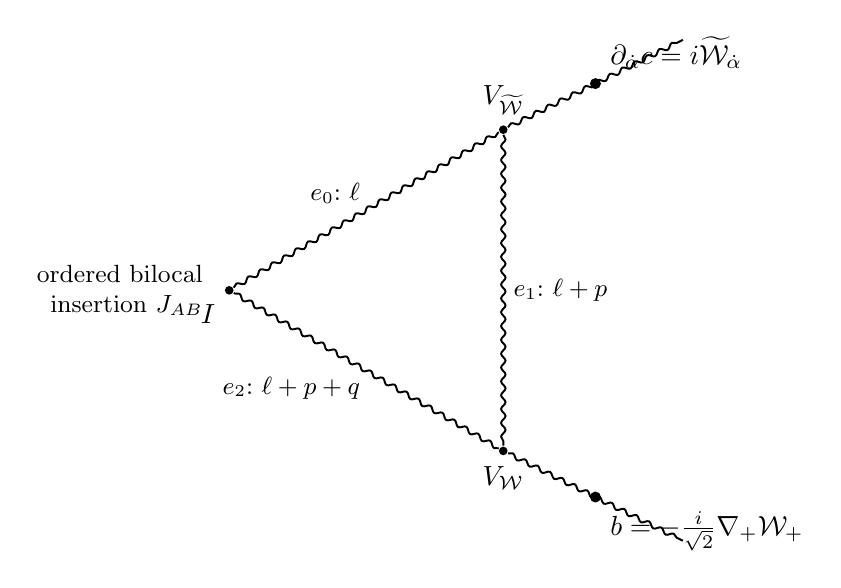
\begin{tikzpicture}[scale=1.2]
  \node[svertex, label=below left:{$I$}] (I) at (0,0) {};
  \node[svertex, label=above:{$V_{\widetilde\cW}$}] (Vt) at (2.9,1.7) {};
  \node[svertex, label=below:{$V_{\cW}$}] (Vw) at (2.9,-1.7) {};
  \draw[sV] (I) -- (Vt) node[midway, above left=-2pt, font=\small] {$e_{0}{:}\ \ell$};
  \draw[sV] (Vt) -- (Vw) node[midway, right, font=\small] {$e_{1}{:}\ \ell+p$};
  \draw[sV] (Vw) -- (I) node[midway, below left=-2pt, font=\small] {$e_{2}{:}\ \ell+p+q$};
  \draw[sV] (Vt) -- ++(1.9,0.95) node[midway, sinsert,
        label=above right:{$\partial_{\dot\alpha}c=i\bcW_{\dot\alpha}$}] {};
  \draw[sV] (Vw) -- ++(1.9,-0.95) node[midway, sinsert,
        label=below right:{$b=-\frac{i}{\sqrt2}\nabla_{+}\cW_{+}$}] {};
  \node[left=4pt of I, font=\small, align=right] {ordered bilocal\\ insertion $J_{AB}$};
\end{tikzpicture}
\caption{The ordered triangle of $(b,\partial_{\dot\alpha}c)$ and
$(\partial_{\dot\alpha}c,b)$. The bilocal insertion $I$ carries the two
letters; $V_{\cW}$ emits the $\nabla_{+}\cW_{+}$ insertion (the $b$ leg) and
$V_{\widetilde\cW}$ the $\bcW_{\dot\alpha}$ insertion (the
$\partial_{\dot\alpha}c$ leg); all internal lines are vector-superfield
propagators. The marked line is $e_{0}$ for $(b,\partial_{\dot\alpha}c)$ and
$e_{2}$ for $(\partial_{\dot\alpha}c,b)$; the Schwinger cut/contact partner
collapses the marked line with the same two vertices.}
\label{fig:ss:ad-triangle}
\end{figure}

The raw engine census per ordering is $36$ TGG $+$ $6$ TMM $+$ $42$ spectator
$=84$ connected $=42_{\rm split\ source}+42_{\rm spectator}$, where TGG (two
gauge cubic vertices) is one ordered triangle of
Figure~\ref{fig:ss:ad-triangle} with a distinguished marked edge, and TMM has
two matter vertices. The occurrence resolution: the $36$ TGG rows per
ordering, with their same-edge Schwinger cuts, carry the entire anomaly (steps
2--6). The $6$ TMM rows vanish exactly (wrong external field type for two
gauge letters). The matter-current Euler and explicit-contact pair shares the
word $K_{\dot1}=ir_{+\dot2}$, $K_{\dot2}=-ir_{+\dot1}$ with weights
$\pm2iK_{\dot\alpha}$ and cancels before regulation; the word is affine, so
its $\mul^{2}$ coefficient vanishes. The source-tagged bubbles have affine
numerators and zero standalone anomaly; their two-denominator rows belong to
the inverse-kernel brackets of step 4 and are not additional finite diagrams.
The tadpole is scaleless, $\int d^{d}\ell\,P(\ell)/\ell^{2}=0$ in DRED
\cite{SiegelDRED}. The gauge-fixing Euler sector cancels the longitudinal
source row (step 4) on $32$ component masks. In the ghost sector, the Euler
bubble and its full-$d$ cut are exact negatives and the ghost kernel is the
full-$d$ $\BoxE$, so no $\mul^{2}$ residue arises; the ghost triangle with
linear source is absent at one loop by the edge/vertex count, and the
Nielsen--Kallosh factor is absent from the selected graph set. The $42$
spectator routes per ordering are connected but one-particle reducible
(external-leg self-energies), and the amputated 1PI projector annihilates
them.

\begin{remark}[Status of the auxiliary sectors]\label{rem:ss:ad-census}
The local Fermi--Feynman proper slice is not derived from first principles; it
is fixed by the scheme decisions of Section~\ref{sec:gaugebv} (Gaussian
averaging; the Nielsen--Kallosh factor kept external). Every contributing
graph is accounted for by the triangle and its same-edge cut; all other
occurrences are exactly zero, cancel in pairs, or are absent.
\end{remark}

\subsubsection*{2. Wick contractions}

The two vertices of~\eqref{eq:ss:ad-vertices} are distinct (one chiral, one
antichiral), so the interaction expansion contributes once at second order:
\begin{equation}\label{eq:ss:ad-wick}
w_{\mathrm{Wick}}=\frac{1}{2!}\,(1+1)=1,
\end{equation}
the $(1+1)$ counting the two equivalent Wick pairings, and the labeled source
Hessian contributes $1!\,1!=1$. There is \emph{no reflection multiplicity}:
$(b,\partial_{\dot\alpha}c)$ (marked edge $e_{0}$) and
$(\partial_{\dot\alpha}c,b)$ (marked edge $e_{2}$) are distinct ordered
descendants, stored separately; the compact output word is already oriented.
The three internal lines contract against the vertices and the source with the
vector propagators of the Fermi--Feynman slice ($\kappa_{AB}=\delta_{AB}$,
Section~\ref{sec:gaugebv}):
\begin{equation}\label{eq:ss:ad-props}
\langle\cV^{A}\cV^{U}\rangle_{e_{0}}
=\frac{\h\,\delta^{AU}\delta^{4}(\theta_{12})}{\ell^{2}},
\qquad
\langle\cV^{C}\cV^{C'}\rangle_{e_{1}}
=\frac{\h\,\delta^{CC'}\delta^{4}(\theta_{12})}{(\ell+p)^{2}},
\qquad
\langle\cV^{V}\cV^{B}\rangle_{e_{2}}
=\frac{\h\,\delta^{VB}\delta^{4}(\theta_{12})}{(\ell+p+q)^{2}} .
\end{equation}
\begin{remark}[Edge-weight sign convention]\label{rem:ss:ad-edgesign}
The edge weights displayed in~\eqref{eq:ss:ad-props} are recorded in the
graph-IR convention of the underlying computation, in which the overall
minus sign of the Feynman propagator $\langle uu\rangle=-\h\kappa^{AB}/p^{2}$
of Section~\ref{sec:superspace:rules} is folded into the vertex signs of the
closed word; the displayed $+\h\kappa^{AB}/p^{2}$ is the edge weight per
line, not an independent propagator sign. All downstream factors of this
subsection use the same convention consistently, and the final coefficients
are machine-verified against the propagator-level replay.
\end{remark}
Contraction with the vertex structure constants and the source yields the
common color tensor in its two allocations, $f^{ACD}f^{BCE}$ (direct) and
$f^{BCD}f^{ACE}$ (crossed), exchanged by $A\leftrightarrow B$ and independent
for a general gauge algebra. The surviving direct ordered source Hessians on
the fixed odd component directions are $i/4$ for $(b,\partial_{\dot\alpha}c)$
and $1/4$ for $(\partial_{\dot\alpha}c,b)$, with $1!\,1!=1$; each external
$\partial_{\dot\alpha}c$ leg carries the component preimage
$-\frac{\sqrt2}{8}\eta_{\dot\alpha}$. Reversing the functional order of the
two odd directions changes the sign of the crossed Hessian, which is why both
color allocations must be kept.

\subsubsection*{3. Amplitude assembly}

The two ordered cubic vertices contribute
$\big(+\frac{ig}{2}\big)\big(-\frac{ig}{2}\big)=\frac{g^{2}}{4}$
as in~\eqref{eq:ss:vertices}, and the closed loop is saturated by
$\delta^{4}(\theta_{12})\cD^{2}\bcD^{2}\delta^{4}(\theta_{12})
=16\,\delta^{4}(\theta_{12})$. The expansion runs over the four chirality
sectors $(++),(+-),(-+),(--)$ of the two vertices, each of weight $1$; the
four contractions coincide polynomially, so the full action contribution is
$4_{\rm chirality}\times(\text{one sector})$. For each occurrence $(\omega,e)$
the frozen source identity splits the marked $D$-algebra word as
\begin{equation}\label{eq:ss:ad-split}
\cD_{-}\cD_{+}\bcD^{2}\cD_{+}
=-8\,\bar r_{e}^{\,2}\,\cD_{+}-\frac12\,\cD_{+}\bcD^{2}\cD^{2},
\end{equation}
so that, writing $\mathscr W^{K}_{\omega,e}$ and $\mathscr W^{L}_{\omega,e}$
for the kinetic and longitudinal spin words,
\begin{equation}\label{eq:ss:ad-kl}
K_{\omega,e}=-8\,\bar r_{e}^{\,2}\,\mathscr W^{K}_{\omega,e},
\qquad
L^{\mathrm{source}}_{\omega,e}=-\tfrac12\,\mathscr W^{L}_{\omega,e},
\qquad
L^{\mathrm{gf}}_{\omega,e}=+\tfrac12\,\mathscr W^{L}_{\omega,e},
\qquad
L^{\mathrm{source}}_{\omega,e}+L^{\mathrm{gf}}_{\omega,e}=0 .
\end{equation}
With $R_{\omega,e}$ the reduced numerator and
$C^{\mathrm{SD}}_{\omega,e}=-R_{\omega,e}/\prod_{j\ne e}D_{j}$ the same-edge
Schwinger contact, the full-$d$ and four-dimensional identities are
\begin{equation}\label{eq:ss:ad-sd}
K^{(d)}_{\omega,e}+C^{\mathrm{SD}}_{\omega,e}=0,
\qquad
K^{(4)}_{\omega,e}+C^{\mathrm{SD}}_{\omega,e}
=\frac{\mul^{2}\,R_{\omega,e}}{D_{0}D_{1}D_{2}},
\end{equation}
the edgewise parent-minus-cut of~\eqref{eq:ss:cuttingfailure}.

\begin{remark}[The factored weight chain is recorded, not displayed]%
\label{rem:ss:ad-weightchain}
Unlike the seed channel, no single displayed chain
$w_{\mathrm{Wick}}\frac{g^{2}}{4}w_{D}$ exists for this family; the total is
fixed by the recorded conversions: a per-chirality conditional factor $-8$, the
absolute conversion
$4_{\rm chirality}\times\big(\tfrac12\big)_{\rm rank/trace}\times
(-8)_{\rm legacy}=-16$,
and the isolating color value $-2$ (the $SU(2)$ sample $(A,B;D,E)=(0,1;1,0)$
gives $(f^{ACD}f^{BCE},f^{BCD}f^{ACE})=(-2,0)$). The rank/trace factor
$\tfrac12$ is inserted exactly once; $m_{\mathrm{contact}}=1$ of step 6
supplies no second factor.
\end{remark}

\subsubsection*{4. The $D$-algebra numerator chain}

With the conditional Fermi--Feynman projector
$\mathcal P_{0}=(\bcD^{2}\cD^{2}+\cD^{2}\bcD^{2})/(16\BoxE)$ and
$\cD_{+}\cD^{2}\bcD^{2}=0$,
\begin{equation}\label{eq:ss:ad-projector}
8\,\cD_{+}\BoxE\,\mathcal P_{0}
=\tfrac12\,\cD_{+}\bcD^{2}\cD^{2}+\tfrac12\,\cD_{+}\cD^{2}\bcD^{2}
=\tfrac12\,\cD_{+}\bcD^{2}\cD^{2},
\end{equation}
so the longitudinal term of~\eqref{eq:ss:ad-split} is pure gauge and cancels
the gauge-fixing Euler row,
$-\tfrac12\cD_{+}\bcD^{2}\cD^{2}+\tfrac12\cD_{+}\bcD^{2}\cD^{2}=0$, verified
sparsely on $32+32$ component masks. What survives is the first term
of~\eqref{eq:ss:ad-split}: per marked edge the parent-minus-cut
of~\eqref{eq:ss:ad-sd} leaves exactly the evanescent
remainder~\eqref{eq:ss:cuttingfailure}. Summing the $36$ TGG routes per
ordering gives the two rank-one route sums
\begin{equation}\label{eq:ss:ad-r12}
R_{1}=\frac{i}{16}\,\mul^{2}\,\Big(\ell+p+\frac12q\Big)_{+\dot1},
\qquad
R_{2}=-\frac{i}{16}\,\mul^{2}\,\ell_{+\dot1},
\end{equation}
with $X_{+\dot1}$ the plus-frame dotted spinor component, and the evanescent
numerators of the two orderings carry the color mix
\begin{equation}\label{eq:ss:ad-nev}
N^{\mathrm{ev}}_{(b,\partial c)}
=f^{ACD}f^{BCE}\,R_{1}+f^{BCD}f^{ACE}\,R_{2},
\qquad
N^{\mathrm{ev}}_{(\partial c,b)}
=f^{ACD}f^{BCE}\,R_{2}+f^{BCD}f^{ACE}\,R_{1},
\end{equation}
the marked edge being $e_{0}$ for the direct $(b,\partial c)$ and crossed
$(\partial c,b)$ rows and $e_{2}$ for the other two. Occurrence by occurrence,
the aggregated two-denominator contact rows and the same-edge remainders obey
\begin{align}
(b,\partial c),\ e_{0}:&\quad
7iq_{+\dot1}+\Big[i\Big(\ell+p+\tfrac12q\Big)_{+\dot1}-7iq_{+\dot1}\Big]
=i\Big(\ell+p+\tfrac12q\Big)_{+\dot1},\notag\\
(b,\partial c),\ e_{1}:&\quad 0+0=0,
\qquad\qquad
(b,\partial c),\ e_{2}:\quad 2iq_{+\dot1}-2iq_{+\dot1}=0,\notag\\
(\partial c,b),\ e_{0}:&\quad
-\tfrac{i}{2}q_{+\dot1}+\tfrac{i}{2}q_{+\dot1}=0,
\qquad\quad
(\partial c,b),\ e_{1}:\quad
i(p+q)_{+\dot1}-i(p+q)_{+\dot1}=0,\notag\\
(\partial c,b),\ e_{2}:&\quad
i(p+q)_{+\dot1}+\big[-i\ell_{+\dot1}-i(p+q)_{+\dot1}\big]
=-i\ell_{+\dot1},
\label{eq:ss:ad-sameedge}
\end{align}
and the crossed-color replay exchanges the two orderings edge by edge. The
two-denominator members of~\eqref{eq:ss:ad-sameedge} belong to the
inverse-kernel brackets and must not be added again as finite diagrams once
$N^{\mathrm{ev}}$ is formed.

\subsubsection*{5. Tensor integrals and the ordered simplex moments}

The two DRED masters are the scalar master~\eqref{eq:ss:masterintegral} and
its rank-one partner,
\begin{equation}\label{eq:ss:ad-masters}
\int\!\frac{d^{d}\ell}{(2\pi)^{d}}\,\frac{\mul^{2}}{D_{0}D_{1}D_{2}}
=\frac{1}{32\pi^{2}},
\qquad
\int\!\frac{d^{d}\ell}{(2\pi)^{d}}\,
\frac{\mul^{2}\,\ell_{+\dot1}}{D_{0}D_{1}D_{2}}
=-\frac{(2p+q)_{+\dot1}}{96\pi^{2}} .
\end{equation}
Combining denominators,
\begin{equation}\label{eq:ss:ad-feynman}
\frac{1}{D_{0}D_{1}D_{2}}
=2\int_{0}^{1}\!dy\int_{0}^{1-y}\!dz\,\frac{1}{(L^{2}+\Delta)^{3}},
\qquad
L=\ell+(y+z)p+zq,
\end{equation}
with exact simplex moments, writing $x=1-y-z$,
\begin{equation}\label{eq:ss:ad-simplex}
2\!\int_{\Delta_{2}}\!1=1,\qquad
2\!\int_{\Delta_{2}}\!x=\frac13,\qquad
2\!\int_{\Delta_{2}}\!(y+z)=\frac23,\qquad
2\!\int_{\Delta_{2}}\!z=\frac13 .
\end{equation}
For $(b,\partial_{\dot\alpha}c)$ the shifted numerator is
$\ell+p+\frac12q=L+xp+\big(\frac12-z\big)q$; the term odd in $L$ integrates to
zero, and $2\int_{\Delta_{2}}(\tfrac12-z)=2(\tfrac14-\tfrac16)=\tfrac16$, so
\begin{equation}\label{eq:ss:ad-adint}
\int_{\ell}\frac{N^{\mathrm{ev}}_{(b,\partial c)}}{D_{0}D_{1}D_{2}}\Big|_{R_{1}}
=\frac{i}{16}\cdot\frac{1}{32\pi^{2}}
\left(\frac13\,p+\frac16\,q\right)_{+\dot1}
=\frac{i}{512\pi^{2}}\left(\frac13\,p+\frac16\,q\right)_{+\dot1} .
\end{equation}
For $(\partial_{\dot\alpha}c,b)$, $-\ell=-L+(y+z)p+zq$ and the
moments~\eqref{eq:ss:ad-simplex} give
\begin{equation}\label{eq:ss:ad-daint}
\int_{\ell}\frac{N^{\mathrm{ev}}_{(\partial c,b)}}{D_{0}D_{1}D_{2}}\Big|_{R_{2}}
=-\frac{i}{16}\left(-\frac{1}{32\pi^{2}}\right)
\left(\frac23\,p+\frac13\,q\right)_{+\dot1}
=\frac{i}{512\pi^{2}}\left(\frac23\,p+\frac13\,q\right)_{+\dot1} ,
\end{equation}
in agreement with the direct evaluation of~\eqref{eq:ss:ad-masters},
$-\frac{i}{16}\big(-\frac{(2p+q)_{+\dot1}}{96\pi^{2}}\big)
=\frac{i}{512\pi^{2}}(\frac23p+\frac13q)_{+\dot1}$. In the authority routing
the raw external momenta are the ordered action ports, $p=k_{L}$ (left output
leg) and $q=k_{R}$ (right output leg). The jet weights of the final bilinear
are the ordered-simplex moments of the tower
parametrization~\eqref{eq:ss:simplexderivation} at $(m,n)=(1,0)$:
\begin{align}
2\int_{0}^{1}\!db\int_{0}^{b}\!da\;a
&=2\int_{0}^{1}\frac{b^{2}}{2}\,db=\frac13
\quad(\text{jet on the first letter}),\notag\\
2\int_{0}^{1}\!db\int_{0}^{b}\!da\;b
&=2\int_{0}^{1}b^{2}\,db=\frac23
\quad(\text{jet on the second letter}),
\label{eq:ss:ad-simplex10}
\end{align}
precisely $K_{1,0;1,0}=\frac{2}{3\cdot2}$ and $K_{1,0;0,0}=\frac{2}{3\cdot1}$
of~\eqref{eq:ss:kernel}. Assembling the four chirality sectors, the two color
allocations and the contact rows, the target-blind momentum shapes are
\begin{align}
\Gamma_{(b,\partial c)}
&=-i\,\frac{\h g^{2}}{16\pi^{2}}\left[
f^{ACD}f^{BCE}\left(\frac13k_{L}+\frac16k_{R}\right)
+f^{BCD}f^{ACE}\left(\frac23k_{L}+\frac13k_{R}\right)\right]_{+\dot1},\notag\\
\Gamma_{(\partial c,b)}
&=-i\,\frac{\h g^{2}}{16\pi^{2}}\left[
f^{ACD}f^{BCE}\left(\frac23k_{L}+\frac13k_{R}\right)
+f^{BCD}f^{ACE}\left(\frac13k_{L}+\frac16k_{R}\right)\right]_{+\dot1}.
\label{eq:ss:ad-shapes}
\end{align}

\begin{remark}[The jet readout is the assembled output, not a Fourier map]%
\label{rem:ss:ad-fourier}
A naive identification of momentum shape with jet weights fails: the
direct-color shape in~\eqref{eq:ss:ad-shapes} is $(\tfrac13,\tfrac16)$, not
$(\tfrac13,\tfrac23)$. The canonical bilinear coefficients of step 7 are the
recorded output of the full four-chirality, two-color, contact-inclusive
assembly, not of a one-line Fourier identification;
\eqref{eq:ss:ad-simplex10} displays the intrinsic jet weights of that
assembled result.
\end{remark}

\subsubsection*{6. Pole cancellation}

The triangle parent and the aggregate Schwinger contact row carry the UV-pole
pair
\begin{align}
\Gamma_{T}&=+\frac{\h g^{2}}{32\pi^{2}\epsilon}\times(\text{edge-tagged
tensor with }\widehat\delta^{mn}),\notag\\
\Gamma_{C}&=-\frac{\h g^{2}}{32\pi^{2}\epsilon}\times(\text{the identical
tensor with }\delta_{4}^{mn}),
\label{eq:ss:ad-polepair}
\end{align}
so the four-dimensional metric parts cancel exactly and the remainder is the
pure evanescent numerator $\widehat\delta^{mn}-\delta_{4}^{mn}
=-\breve\delta^{mn}$, whose sigma-trace supplies the $-2\epsilon$
of~\eqref{eq:ss:sigmatrace}: finiteness holds precisely as in
Remark~\ref{rem:ss:polebookkeeping}. At the occurrence level, the local
contact kernel $K_{AB}=-\kappa_{AB}r_{e}^{2}$ with
$\kappa_{AB}=\tfrac12\delta_{AB}$ obeys $r_{e}^{2}P^{A}=-2P^{A}K_{A}$, and
\begin{align}
c_{\mathrm{parent}}&=(-2)^{3}=-8,
\qquad
c_{\mathrm{contact}}
=(-1)_{\mathrm{SD}}\,(-2)_{r^{2}P=-2PK}\,(-2)^{2}_{\mathrm{uncut}}=+8,\notag\\
m_{\mathrm{contact}}
&=\Big(\tfrac{1}{2!}\,2_{\mathrm{action}}\Big)
\Big(\tfrac{1}{2!}\,2_{\mathrm{cut}}\Big)
\Big(\tfrac{1}{2!}\,2_{\mathrm{Wick}}\Big)=1 .
\label{eq:ss:ad-signs}
\end{align}
Consequently, occurrence by occurrence and in each chirality sector,
\begin{equation}\label{eq:ss:ad-occcancel}
N^{\mathrm{parent}}_{d,\omega}+K^{\mathrm{contact}}_{\mathrm{raw},\omega}=0,
\qquad
N^{\mathrm{parent}}_{4,\omega}+K^{\mathrm{contact}}_{\mathrm{raw},\omega}
=\frac{R_{\omega}\,\mul^{2}}{D_{0}D_{1}D_{2}} .
\end{equation}
The finite-$w$ link sector cancels before loop integration: with $x=iwr$,
$y=iwr'$ and $(x-y)\int_{0}^{1}ds\,e^{sx+(1-s)y}=e^{x}-e^{y}$, the one-link
term and the two endpoint terms cancel,
$C_{\omega,e}(e^{x}-e^{y})-C_{\omega,e}(e^{x}-e^{y})=0$; the sector is
longitudinal in arbitrary $d$, so its $\mul^{2}$ coefficient is exactly zero.

\subsubsection*{7. The final coefficients and the tower-kernel instance}

With unit-normalized insertions the assembled channel results are
\begin{align}
\nabla_{-}\big((\nabla_{+}\cW_{+})^{A}\,\bcW_{\dot\alpha}^{B}\big)
&=\frac{\h g^{2}}{16\pi^{2}}\,f^{ACD}f^{BCE}\,
\Big\{\tfrac13\big\langle\partial_{\dot\alpha}\bcW,\bcW\big\rangle
+\tfrac23\big\langle\bcW,\partial_{\dot\alpha}\bcW\big\rangle\Big\}^{DE},
\label{eq:ss:ad-unit1}\\
\nabla_{-}\big(\bcW_{\dot\alpha}^{A}\,(\nabla_{+}\cW_{+})^{B}\big)
&=\frac{\h g^{2}}{16\pi^{2}}\,f^{ACD}f^{BCE}\,
\Big\{\tfrac23\big\langle\partial_{\dot\alpha}\bcW,\bcW\big\rangle
+\tfrac13\big\langle\bcW,\partial_{\dot\alpha}\bcW\big\rangle\Big\}^{DE}.
\label{eq:ss:ad-unit2}
\end{align}
Restoring the letters of Definition~\ref{def:ss:letters} is exact arithmetic:
the insertions and the output letters give
\begin{align}
b^{A}\,\partial_{\dot\alpha}c^{B}
&=\Big(-\frac{i}{\sqrt2}\Big)(i)\,
(\nabla_{+}\cW_{+})^{A}\,\bcW_{\dot\alpha}^{B}
=\frac{1}{\sqrt2}\,(\nabla_{+}\cW_{+})^{A}\,\bcW_{\dot\alpha}^{B},
\notag\\
\big\langle\partial_{\dot\alpha}\bcW,\bcW\big\rangle
&=(-i)^{2}\,\big\langle\partial_{\dot\alpha}(\partial c),\partial c\big\rangle ,
\label{eq:ss:ad-restore}
\end{align}
and $\frac{1}{\sqrt2}\times(-1)\times\frac{\h g^{2}}{16\pi^{2}}
=-\frac{\h g^{2}}{16\sqrt2\,\pi^{2}}$. Substituting
into~\eqref{eq:ss:ad-unit1}--\eqref{eq:ss:ad-unit2},
\begin{equation}\label{eq:ss:ad-bdc}
\boxed{\begin{aligned}
\nabla_{-}\big(b^{A}\partial_{\dot\alpha}c^{B}\big)
&=-\frac{\h g^{2}}{16\sqrt2\,\pi^{2}}\,f^{ACD}f^{BCE}\\
&\quad\times
\Big\{\tfrac13\big\langle\partial_{\dot\alpha}(\partial c),\partial c\big\rangle
+\tfrac23\big\langle\partial c,\partial_{\dot\alpha}(\partial c)\big\rangle
\Big\}^{DE}
\end{aligned}}
\end{equation}
\begin{equation}\label{eq:ss:ad-dcb}
\boxed{\begin{aligned}
\nabla_{-}\big(\partial_{\dot\alpha}c^{A}b^{B}\big)
&=-\frac{\h g^{2}}{16\sqrt2\,\pi^{2}}\,f^{ACD}f^{BCE}\\
&\quad\times
\Big\{\tfrac23\big\langle\partial_{\dot\alpha}(\partial c),\partial c\big\rangle
+\tfrac13\big\langle\partial c,\partial_{\dot\alpha}(\partial c)\big\rangle
\Big\}^{DE}
\end{aligned}}
\end{equation}
--- exactly the rows~\eqref{eq:ss:ch-bdc} and~\eqref{eq:ss:ch-dcb} of the
channel table. The weights are the $(m,n)=(1,0)$ instance of the tower
kernel~\eqref{eq:ss:kernel}: by~\eqref{eq:ss:ad-simplex10},
$K_{1,0;1,0}=\frac{2}{3\cdot2}=\frac13$ (jet on the first letter) and
$K_{1,0;0,0}=\frac{2}{3\cdot1}=\frac23$ (jet on the second), and the two
orderings are exchanged by the Leibniz distribution
$(1,1)-(\tfrac13,\tfrac23)=(\tfrac23,\tfrac13)$.

\begin{remark}[No $1:2$ ratio between the two orderings]\label{rem:ss:ad-ratio}
An earlier conditional proposal assigned the two orderings the ratio
$\mathcal N_{(b,\partial c)}/\mathcal N_{(\partial c,b)}=1/2$ through a
rejected momentum map; it was explicitly \emph{not} promoted to a coefficient
of this paper. The final results~\eqref{eq:ss:ad-bdc}--\eqref{eq:ss:ad-dcb}
share the single prefactor
$-\frac{\h g^{2}}{16\sqrt2\,\pi^{2}}f^{ACD}f^{BCE}$ and differ only in the
jet weights $(\tfrac13,\tfrac23)\leftrightarrow(\tfrac23,\tfrac13)$.
\end{remark}

\begin{remark}[Machine cross-checks for this family]\label{rem:ss:ad-checks}
The full chain of this subsection was replayed externally: $94/94$ checks on
the ordered-port crossed-Hessian assembly, $112/112$ on each of the two
polarized $D$-algebra replays, and $255/255$ on the raw contact and finite-$w$
link replay, with zero failures.
\end{remark}

\subsubsection*{8. Comparison with the holomorphic twist}

In the holomorphic twist of~\cite{BK} this family has no zero-derivative
display; it exists only through the derivative tower applied to the seed pair
$Q_{1}(b^{A}c^{B})
=\kappa_{H}^{2}f_{ACD}f_{BCE}\,\partial_{\dot\alpha}c^{D}
\partial^{\dot\alpha}c^{E}$ (their eq.~(3.63)). Their Appendix-B tower
(their eq.~(B.6)),
\begin{align}
Q_{1}\big(b^{A}\partial_{1}^{m}\partial_{2}^{n}c^{B}\big)
&=\kappa_{H}^{2}f_{ACD}f_{BCE}\,\frac{1}{m+n+2}
\sum_{k=0}^{m}\sum_{\ell=0}^{n}\frac{1}{k+\ell+1}\binom{m}{k}\binom{n}{\ell}
\notag\\
&\quad\times
\big[\partial_{1}^{k}\partial_{2}^{\ell}\partial_{\dot\alpha}c^{D}\,
\partial_{1}^{m-k}\partial_{2}^{\,n-\ell}\partial^{\dot\alpha}c^{E}\big],
\label{eq:ss:ad-bktower}
\end{align}
evaluated at $(m,n)=(1,0)$, gives the printed weights
\begin{align}
k=0:&\quad \frac13\ \text{on}\ \partial_{\dot\alpha}c^{D}\,
\partial_{1}\partial^{\dot\alpha}c^{E}\ (\text{jet on the second letter}),
\notag\\
k=1:&\quad \frac16\ \text{on}\ \partial_{1}\partial_{\dot\alpha}c^{D}\,
\partial^{\dot\alpha}c^{E}\ (\text{jet on the first letter}),
\label{eq:ss:ad-bkweights}
\end{align}
exactly one half of our coefficients on both words. After the factor-two
adjudication of Section~\ref{sec:ht} --- the printed Appendix-B branch
of~\cite{BK} is uniformly smaller by the factor $2=\Gamma(3)$
of~\eqref{eq:ss:feynman} --- the corrected weights $(\tfrac13,\tfrac23)$
coincide with~\eqref{eq:ss:ad-bdc}. The reversed ordering
$(\partial_{\dot\alpha}c,b)$ is not printed in~\cite{BK} at all; it follows
from their recursion (their eq.~(B.1)),
$Q_{1}(\partial_{\dot\alpha}fg)
=\partial_{\dot\alpha}Q_{1}(fg)-Q_{1}(f\,\partial_{\dot\alpha}g)$, applied to
$(f,g)=(c,b)$, the unprinted orderings being identified with the printed ones
by supercommutativity of the letters (no sign, since $|c||b|=0$). On our side
the same law is the Leibniz distribution on the formal ghost slot: the seed
distributes one unit of weight on each output word, $(1,1)$, and
$(1,1)-(\tfrac13,\tfrac23)=(\tfrac23,\tfrac13)$, exactly the swap
between~\eqref{eq:ss:ad-bdc} and~\eqref{eq:ss:ad-dcb}. Both dotted rows agree
word by word with the twist computation (Section~\ref{sec:ht}).

\begin{remark}[Status of the ghost-slot recursion]\label{rem:ss:ad-Uslot}
The recursion anchor involves the formal odd slot of the twist dictionary (the
ghost placeholder, of parity $1$), whose identification with project
quantities is conditional; the physical
rows~\eqref{eq:ss:ad-bdc}--\eqref{eq:ss:ad-dcb} are derived independently in
steps 1--7 and are unaffected. The comparison of this subsection is a
cross-check, not a derivation input, and not a completeness proof of the graph
census (Section~\ref{sec:ht}).
\end{remark}

% sec04f-bb.tex — Section 4 subsection: the (beta_r, beta_s) channel
% Writer: 作家_BB (Writer_BB). Body LaTeX only; macros live in main.tex.

\subsection{The channel $(\beta_r,\beta_s)$}\label{sec:superspace:bb}

We now compute the $(\beta_r,\beta_s)$ family in full: the six ordered
off-diagonal channels $r\ne s$ of the census~\eqref{eq:ss:29} and the three
diagonal zeros. The result is the row~\eqref{eq:ss:ch-betabeta} of the channel
table, derived here graph by graph. As in the seed channel
(Section~\ref{sec:superspace:seed}), all graph weights are evaluated with
unit-normalized letters
\begin{equation}\label{eq:ss:bb-unit}
B_r:=\sqrt2\,\beta_r,\qquad C^t:=\gamma^t,\qquad D_{\dot\alpha}:=-i\,\partial_{\dot\alpha}c,
\end{equation}
and the normalization of Definition~\ref{def:ss:letters} is restored at the
end. In these letters the two ordered output carriers are
\begin{equation}\label{eq:ss:bb-carriers}
A_1:=\langle D^{\,D},C^{t\,E}\rangle,\qquad
A_2:=\langle C^{t\,D},D^{\,E}\rangle,
\end{equation}
onto which every graph is projected without quotienting by total derivatives
or exchanging the color indices $D,E$.

\paragraph{1. The insertion and the descendant.} With the absorbed-frame
scalings $\Phi_r=g\phi_r$, $\widetilde\Phi^r=g\widetilde\phi^r$ and the
unit-normalized prepotential $u$, $\cV=\sqrt2 g\,u$, the gauge-covariant
letter source expands as
\begin{equation}\label{eq:ss:bb-resolvent}
B_{r,c}=\cD_+\phi_r+g\sqrt2\,[\cD_+u,\phi_r]
+g^2\big[(\cD_+u)u-u(\cD_+u),\phi_r\big]+O(g^3),
\end{equation}
so the leading insertion of the channel is
\begin{equation}\label{eq:ss:bb-insertion}
\mathcal O^{(0),AB}_{B_rB_s}=g^{2}\,(\cD_+\phi_r)^{A}(\cD_+\phi_s)^{B}.
\end{equation}
The descendant of one letter follows from the tree
system~\eqref{eq:ss:treeduction}:
\begin{equation}\label{eq:ss:bb-descendant}
\nabla_-B_r=-2\,\frac{\delta S}{\delta\widetilde\Phi^{r}}
-\sqrt2\,\varepsilon_{rst}\,(C^{s}\times C^{t}),
\qquad
\frac{\delta S}{\delta\widetilde\Phi^{r}}
=-\frac14\nabla^{2}\Phi_r-\frac{1}{\sqrt2}\,\varepsilon_{rst}\,(C^{s}\times C^{t}),
\end{equation}
with $(X\times Y)^A=f^{ABC}X^BY^C$ as in Section~\ref{sec:superspace:sd}.

\begin{remark}[No pre-simplification before the occurrence census]%
\label{rem:ss:bbnopresimplify}
The two potential structures in~\eqref{eq:ss:bb-descendant} --- the
Euler-potential piece $+\sqrt2\,\varepsilon_{rst}(C^s\times C^t)$ contained in
$-2\,\delta S/\delta\widetilde\Phi^r$ and the explicit piece
$-\sqrt2\,\varepsilon_{rst}(C^s\times C^t)$ --- carry opposite signs and equal
regulated kernels, and they cancel only \emph{after} the regulated occurrence
census of paragraph~7. It is not legitimate to pre-simplify
\eqref{eq:ss:bb-descendant} to $\tfrac12\nabla^2\Phi_r$ before that census:
doing so erases the Euler-potential occurrence and corrupts the pole
bookkeeping of Remark~\ref{rem:ss:polebookkeeping}.
\end{remark}

\paragraph{2. Graph inventory.} The amputated ordered coefficient receives
contributions from exactly three triangle parents. For $r\ne s$ with
$\varepsilon_{rst}\ne0$ they are: the two-matter-vertex triangle (TMM, ports
$(\phi_r,\phi_s)$), and the two matter/superpotential triangles (TMH), route
002 with vertices $(M_r,H_-)$ and external ports $(u^D,\widetilde\phi^{tE})$,
route 003 with vertices $(H_-,M_s)$ and ports $(\widetilde\phi^{tD},u^E)$.
Route 003 is computed as an independent orientation --- reversed ports and
graded source order --- never inferred from route 002 by reflection. All three
internal lines of every triangle are matter lines
$\langle\phi\widetilde\phi\rangle$; the external legs are one gauge leg $u^D$
and one antichiral matter leg $\widetilde\phi^{tE}$, the residual external
operators that the external map of paragraph~4 converts to the letters
$\partial c$ and $\gamma^t$. The momentum routings are
\begin{equation}\label{eq:ss:bb-routing}
r_0=\ell,\quad r_1=\ell-p,\quad r_2=\ell-p-q;
\qquad
\rho_0=\ell,\quad \rho_1=\ell-q,\quad \rho_2=\ell-p-q,
\end{equation}
for routes 002 and 003 respectively, with the canonical loop rebase
\begin{equation}\label{eq:ss:bb-rebase}
k_0=-\rho_2,\qquad k_1=-\rho_1=k_0-p,\qquad k_2=-\rho_0=k_0-p-q,
\end{equation}
and the kinematic bookkeeping
\begin{equation}\label{eq:ss:bb-kinematics}
D_i=r_{i,d}^{2},\qquad \bar r_i^{\,2}=r_{i,d}^{2}+\mul^{2},\qquad \det r_i=-\bar r_i^{\,2},
\end{equation}
where $p$ is the external momentum at the matter vertex and $q$ the external
momentum at $H_-$. The triangle of route 002 is displayed in
Figure~\ref{fig:ss:bbtriangle}.

\begin{figure}[t]
\centering
\begin{tikzpicture}[scale=1.25]
  \node[sinsert] (O) at (0,0) {};
  \node[below=3pt of O, font=\small] {$\mathcal O_{B_rB_s}^{(0)}$};
  \node[svertex] (M) at (-2.2,2.1) {};
  \node[left=3pt of M, font=\small] {$M_r$};
  \node[svertex] (H) at (2.2,2.1) {};
  \node[right=3pt of H, font=\small] {$H_-$};
  \draw[sV] (M) -- ++(-1.15,0.85) node[left, font=\small] {$u^{D}\ (p)$};
  \draw[sPhit] (H) -- ++(1.15,0.85) node[right, font=\small] {$\widetilde\phi^{tE}\ (q)$};
  \draw[sPhi] (O) -- node[pos=0.5, left, font=\small] {$r_0=\ell$} (M);
  \draw[sPhi] (M) -- node[pos=0.5, above, font=\small] {$r_1=\ell-p$} (H);
  \draw[sPhi] (H) -- node[pos=0.5, right, font=\small] {$r_2=\ell-p-q$} (O);
\end{tikzpicture}
\caption{The ordered triangle of route 002 for the $(\beta_r,\beta_s)$
channel, $r\ne s$, drawn in the unit normalization~\eqref{eq:ss:bb-unit}. The
composite insertion $\mathcal O_{B_rB_s}^{(0)}$ (filled node) attaches to the
matter vertex $M_r$ and to the superpotential vertex $H_-$; the three internal
lines are chiral--antichiral matter propagators with the displayed routing;
the external legs are the unit prepotential $u^D$ (wavy) and the antichiral
field $\widetilde\phi^{tE}$, converted to the letters $\partial c$ and
$\gamma^t$ by the external map~\eqref{eq:ss:bb-extmap}. Route 003 is the
independently oriented partner with reversed ports and the
rebase~\eqref{eq:ss:bb-rebase}.}
\label{fig:ss:bbtriangle}
\end{figure}

Beyond the triangles, the family contains: (a) two-point contact rows of
bubble topology, the $\langle I_1S_{H_-}\rangle$ rows $T_2,T_4$ of paragraph~7,
where $I_1$ is the $O(g)$ commutator term of~\eqref{eq:ss:bb-resolvent};
(b) the Euler-kinetic cut rows of paragraph~7; (c) the Euler-potential and
explicit-potential rows of Remark~\ref{rem:ss:bbnopresimplify}, which cancel
each other before integration. Everything else vanishes exactly or is
excluded: the twelve $I_2$ rows have no antichiral port; the $I_0S_4$ matter
rows cannot absorb both flavors $r,s$, and $H_-$ has no quartic vertex; the
gauge-fixing, ghost and auxiliary rows have no pair of matter-flavor ports;
the coincident Jacobian contains $\delta_{rs}=0$ for $r\ne s$; and the four
spectator double-bridge parents (vertex pairs $(H_-,H_+)$ or $(M,M)$ with one
letter as spectator) all have the source edge as an articulation edge, so they
are one-particle-reducible external self-energy attachments and do not enter
the amputated coefficient.

\paragraph{3. Wick contractions.} With the Euclidean exponent $e^{-S/\h}$ the
vertex factors are $+\sqrt2 g/\h$ for $M_r$ and
$-\sqrt2 g\,\varepsilon_{rst}/\h$ for $H_-$, and the propagators are
\begin{equation}\label{eq:ss:bb-propagators}
\langle u^{A}u^{B}\rangle=-\frac{\h\,\delta^{AB}}{p^{2}}\,\delta^{4}(\theta_{12}),
\qquad
\langle\phi_r^{A}\widetilde\phi^{sB}\rangle
=\delta_r{}^{s}\,\frac{\h\,\delta^{AB}}{16\,p^{2}}\,
\bcD_1^{2}\cD_1^{2}\,\delta^{4}(\theta_{12}),
\end{equation}
with the reversed chiral-line orientation derived explicitly rather than by
reflection. The finite-Grassmann expansion of each triangle has two possible
outer marks, according to which source edge carries the descendant
$\nabla_-$-word of~\eqref{eq:ss:bb-descendant}. The marks are sparse:
\begin{equation}\label{eq:ss:bb-marks}
R_{001,L}=R_{001,R}=0,\qquad
R_{002,L}=0,\quad R_{002,R}=128\,v(r_0),\qquad
R_{003,R}=0,\quad R_{003,L}=-128\,v(\rho_2)=128\,v(k_0),
\end{equation}
where $v(k):=(-k_{+\dot2},\,k_{+\dot1})$ and the surviving mark of route 002
sits on the $B_s$ source edge (selected edge $r_2$), that of route 003 on the
$B_r$ source edge (selected edge $k_2$ after the
rebase~\eqref{eq:ss:bb-rebase}). Explicitly, the raw parent word before the
selected inverse-kernel square is removed is
$R^{\dot1}=-1024\,r_{0,+\dot2}\det r_2$,
$R^{\dot2}=+1024\,r_{0,+\dot1}\det r_2$, and removing the selected square
leaves the residual word $128\,v(r_0)=(-128\,r_{0,+\dot2},128\,r_{0,+\dot1})$.
The TMM route 001 has both marks zero and drops out. The contraction
multiplicity is the Taylor/ordering factor
\begin{equation}\label{eq:ss:bb-taylor}
\frac{1}{2!}\,(1+1)=1,
\end{equation}
the second-order Taylor coefficient times the two vertex orderings. The color
contraction of route 002 gives $+f^{ACD}f^{BCE}$, that of route 003 gives
$-f^{ACD}f^{BCE}$; including the Koszul and source-attachment signs, the net
route signs multiplying the common $+f^{ACD}f^{BCE}$ are
\begin{equation}\label{eq:ss:bb-routesigns}
s_{002}=-i,\qquad s_{003}=+i .
\end{equation}

\begin{remark}[Sign bookkeeping]\label{rem:ss:bbsignchain}
The color and sign outcomes~\eqref{eq:ss:bb-routesigns} are quoted at the
granularity at which they were machine-verified (contraction value, ports,
selected edge, net sign per route); we do not display an intermediate
term-by-term sign chain. The quoted color outcomes and route signs are
independent machine-checked rows, not a displayed factorization: the
effective multiplier of the common $+f^{ACD}f^{BCE}$ is $s_{00n}$, with the
color-contraction sign folded into it.
\end{remark}

\paragraph{4. Prefactors and the external map.} Assembling the vertex factors,
propagator numerators and the multiplicity~\eqref{eq:ss:bb-taylor}, the
triangle and contact prefactors are
\begin{equation}\label{eq:ss:bb-prefactors}
P_\triangle
=g^{2}\Big(\frac{\sqrt2 g}{\h}\Big)\Big(-\frac{\sqrt2 g}{\h}\Big)
\Big(\frac{\h}{16}\Big)^{3}\frac{1}{2!}(1+1)
=-\frac{\h g^{4}}{2048},
\qquad
P_{I_1H}
=g^{2}(\sqrt2 g)\Big(-\frac{\sqrt2 g}{\h}\Big)\Big(\frac{\h}{16}\Big)^{2}
=-\frac{\h g^{4}}{128}.
\end{equation}
The factors read: $g^2$ from the two source legs; one $M$ vertex and one $H_-$
vertex; three chiral propagators $(\h/16)^3$ in the triangle; in $P_{I_1H}$
the $O(g)$ commutator $\sqrt2[\cD_+u,\phi_r]$ of one insertion supplies
$\sqrt2 g$, one $H_-$ vertex, and two chiral propagators. For the external
legs, the source probe $u_{\dot\alpha}=\theta^+\theta^-\bar\theta_{\dot\alpha}$
gives
\begin{equation}\label{eq:ss:bb-extmap}
\cD^{2}\bcD_{\dot\alpha}u_{\dot\alpha}\big|=-2,
\qquad
\cD^{2}\bcD_{\dot\alpha}u\big|=-\frac{4\sqrt2}{g}\,D_{\dot\alpha},
\qquad
C^{t}=g\,\widetilde\phi^{t},
\qquad
M_{\mathrm{ext}}=\frac{2\sqrt2}{g^{2}},
\end{equation}
i.e. the probe ratio $(-4\sqrt2/g)/(-2)=2\sqrt2/g$ expresses the gauge leg
through the letter $D_{\dot\alpha}$, and $\widetilde\phi^t=g^{-1}C^t$
expresses the antichiral leg through $C^t$. Each nonzero row then assembles as
\begin{equation}\label{eq:ss:bb-assembly}
\Gamma_{\mathrm{row}}
=P\times N^{\mathrm{ev}}\times
\int_{\ell}^{\mathrm{DRED}}\frac{\mul^{2}}{D_0D_1D_2}
\times M_{\mathrm{ext}}\times\big(s_{00n}\,f^{ACD}f^{BCE}\big),
\end{equation}
with $P\in\{P_\triangle,P_{I_1H}\}$, the evanescent word $N^{\mathrm{ev}}$ of
paragraph~6, and the simplex weights decomposing the result onto the
carriers~\eqref{eq:ss:bb-carriers}.

\paragraph{5. $D$-algebra chain.} Let $\Pi_b$ be the bridge projector (edge
$r_1$) and $\Pi_s$ the source-edge projector; both are Grassmann-even. Since
$\cD^{2}=2\cD_-\cD_+$, the Leibniz rule gives the complete identity
\begin{equation}\label{eq:ss:bb-productrule}
\cD^{2}(\Pi_b\Pi_s)
=(\cD^{2}\Pi_b)\Pi_s+\Pi_b(\cD^{2}\Pi_s)
+2(\cD_-\Pi_b)(\cD_+\Pi_s)-2(\cD_+\Pi_b)(\cD_-\Pi_s).
\end{equation}
In the ordered $(u,\widetilde\phi^{t})$ projection the first and third terms
vanish,
\begin{equation}\label{eq:ss:bb-survivors}
(\cD^{2}\Pi_b)\Pi_s=0,\qquad 2(\cD_-\Pi_b)(\cD_+\Pi_s)=0,
\end{equation}
leaving the two survivors $\Pi_b(\cD^{2}\Pi_s)$ and
$-2(\cD_+\Pi_b)(\cD_-\Pi_s)$. The pure-antichiral endpoint is
\begin{equation}\label{eq:ss:bb-endpoint}
\theta^{2}=-2\theta^{+}\theta^{-},
\qquad
\boxed{\;\cD^{2}\theta^{2}=-4\;}.
\end{equation}
For route 002 the direct core before the endpoint is
$N_{\mathrm{core},002}^{\mathrm{dir}}=1024\,v(r_0)\det r_2$, and the two
survivors collapse exactly to
\begin{equation}\label{eq:ss:bb-route002}
\Pi_b(\cD^{2}\Pi_s)\longmapsto(-4)\cdot1024\,v(r_0)\det r_2
=4096\,v(r_0)\,\bar r_2^{2},
\qquad
-2(\cD_+\Pi_b)(\cD_-\Pi_s)\longmapsto-2048\,v(r_0)\det r_1
=2048\,v(r_0)\,\bar r_1^{2},
\end{equation}
using $\det r_i=-\bar r_i^{\,2}$. Thus the channel has \emph{two occurrences}
per oriented route: the direct occurrence on edge $e=2$ and the transported
occurrence on the bridge edge $e=1$, with ratio
\begin{equation}\label{eq:ss:bb-ratio}
\frac{O^{\mathrm{tr}}}{O^{\mathrm{dir}}}=\frac{-2}{-4}=\frac12 .
\end{equation}
For route 003, computed in its independent orientation, the cores are
\begin{equation}\label{eq:ss:bb-route003}
N_{\mathrm{core},003}^{\mathrm{dir}}=-1024\,v(\rho_2)\det\rho_0
=1024\,v(k_0)\det k_2,
\qquad
N_{\mathrm{core},003}^{\mathrm{tr}}=+2048\,v(\rho_2)\det\rho_1,
\end{equation}
and using $v(\rho_2)=-v(k_0)$ and $\det\rho_j=\det k_{2-j}$ the endpoint words
are $4096\,v(k_0)\bar k_2^{2}$ (direct, edge $k_2$) and $2048\,v(k_0)\bar
k_1^{2}$ (transported, edge $k_1$). The single-projector identity
\begin{equation}\label{eq:ss:bb-projectorid}
\cD^{2}\bcD^{2}\cD^{2}\delta^{4}=16\det(r)\,\cD^{2}\delta^{4}
\end{equation}
does not delete the neighboring occurrence, because
\begin{equation}\label{eq:ss:bb-projectorid2}
\cD_+\bcD^{2}\cD^{2}\delta^{4}
=16\det(r)\,\cD_+\delta^{4}-\cD^{2}\bcD^{2}\cD_+\delta^{4}.
\end{equation}

\paragraph{6. Evanescent extraction and tensor reduction.} For every selected
edge $e$, the full-$d$ Schwinger--Dyson pair cancels identically,
\begin{equation}\label{eq:ss:bb-sdpair}
\frac{r_{e,d}^{2}R_e}{D_0D_1D_2}-\frac{R_e}{\prod_{j\ne e}D_j}=0,
\end{equation}
and in DRED the cutting-failure identity~\eqref{eq:ss:cuttingfailure} leaves
the universal remainder
\begin{equation}\label{eq:ss:bb-dredremainder}
\frac{\bar r_e^{\,2}R_e}{D_0D_1D_2}-\frac{R_e}{\prod_{j\ne e}D_j}
=\frac{\mul^{2}R_e}{D_0D_1D_2}.
\end{equation}
The direct and transported evanescent words are therefore
\begin{equation}\label{eq:ss:bb-evanescent}
N^{\mathrm{ev}}_{\mathrm{dir}}=4096\,\mul^{2}v(r_0),
\qquad
N^{\mathrm{ev}}_{\mathrm{tr}}=2048\,\mul^{2}v(r_0),
\end{equation}
and identically on route 003 with $v(r_0)\to v(k_0)$ and edges $k_2,k_1$. The
ordered-simplex moments with the $\Gamma(3)=2$ measure are
\begin{equation}\label{eq:ss:bb-simplex}
2\int_{\Sigma_2}1=1,\qquad 2\int_{\Sigma_2}y=\frac13,\qquad 2\int_{\Sigma_2}z=\frac13,
\end{equation}
and with $r_0=L+yp+z(p+q)$, respectively $k_0=L+yp+z(p+q)$ after the
rebase~\eqref{eq:ss:bb-rebase},
\begin{equation}\label{eq:ss:bb-shift}
2\int_{\Sigma_2}r_0=\frac23\,p+\frac13\,q,
\qquad
2\int_{\Sigma_2}k_0=\frac23\,p+\frac13\,q .
\end{equation}
The rank-one numerator $v(r_0)$ thereby reduces onto the ordered
carriers~\eqref{eq:ss:bb-carriers} as
\begin{equation}\label{eq:ss:bb-carrierreduction}
\text{route }002:\ \tfrac23 A_1+\tfrac13 A_2,
\qquad
\text{route }003:\ \tfrac13 A_1+\tfrac23 A_2,
\end{equation}
where the reversed ports of route 003 place $q/3$ on $A_1$ and $2p/3$ on
$A_2$. No factor $p^{2},\bar p^{2},q^{2},\bar q^{2}$ multiplies these
carriers, so no external-equation-of-motion admixture survives: the contact
rows $E_1,E_2$ vanish by the external equations of motion
($\bar q^{2}-q_d^{2}=0$, $\bar p^{2}-p_d^{2}=0$), and $T_1,T_3$ vanish by
spinor-derivative nilpotence ($\cD_+^{2}=0$).

\paragraph{7. Pole cancellation.} The transported occurrence cancels against
the $\langle I_1S_{H_-}\rangle$ contact row of its own route. The prefactor
arithmetic is
\begin{equation}\label{eq:ss:bb-polecancel}
P_\triangle(2048)+P_{I_1H}(-128)=-\h g^{4}+\h g^{4}=0,
\end{equation}
so the full-$d$ bubble pole cancels pointwise, before integration:
\begin{equation}\label{eq:ss:bb-pointwise}
P_\triangle\,\frac{2048\,r_{1,d}^{2}v(r_0)}{D_0D_1D_2}
+P_{I_1H}\,\frac{-128\,v(r_0)}{D_0D_2}=0,
\end{equation}
leaving only the evanescent remainder
\begin{equation}\label{eq:ss:bb-tremainder}
P_\triangle\,\frac{2048\,\mul^{2}v(r_0)}{D_0D_1D_2}.
\end{equation}
Indeed, writing $\bar r_1^{2}=r_{1,d}^{2}+\mul^{2}$ in the transported
occurrence, the $r_{1,d}^{2}$ part cancels $D_1$ and lands exactly on the
contact row $T_2=-128\,v(r_0)/(D_0D_2)$ with the matching
prefactors~\eqref{eq:ss:bb-polecancel}; route 003 is identical with
$T_4=-128\,v(k_0)/(K_0K_2)$ on the edge $k_1$. The two contact rows cannot be
merged into one untagged polynomial: $T_2$ carries color $+if^{ACD}f^{BCE}$,
ports $(u^D,C^{tE})$ and edge $r_1$, while $T_4$ carries $-if^{ACD}f^{BCE}$,
ports $(C^{tD},u^E)$ and edge $k_1$; each cancels its own route's transported
occurrence. For the direct occurrence, the full-$d$ pair~\eqref{eq:ss:bb-sdpair}
applies with $R_e=4096\,v(r_0)$: the parent term
$4096\,v(r_0)r_{2,d}^{2}/(D_0D_1D_2)$ is cancelled by the Euler-kinetic cut
row, whose regulated word is
\begin{equation}\label{eq:ss:bb-eulercut}
-4096\,v(r_0)/(D_0D_1)\ \ \text{(route 002)},
\qquad
-4096\,v(k_0)/(K_0K_1)\ \ \text{(route 003)},
\end{equation}
an Euler-operator insertion collapsing its propagator by the cutting rule
$KK^{-1}=\delta$ of Section~\ref{sec:superspace:cutting}, leaving the DRED
remainder $4096\,\mul^{2}v(r_0)/(D_0D_1D_2)$. Finally, the Euler-potential and
explicit-potential rows of Remark~\ref{rem:ss:bbnopresimplify} have identical
regulated kernels and opposite signs,
\begin{equation}\label{eq:ss:bb-potcancel}
\big(+\sqrt2\,K_{\mathrm{potential}}\big)+\big(-\sqrt2\,K_{\mathrm{potential}}\big)=0,
\end{equation}
and cancel before integration.

\begin{remark}[Granularity of the cut row]\label{rem:ss:bbeulercut}
The Euler-kinetic cut is presented through the universal Schwinger--Dyson
identity~\eqref{eq:ss:bb-sdpair} together with the recorded contact
word~\eqref{eq:ss:bb-eulercut}; no standalone prefactor formula for this row
exists in the underlying computation, and none is needed, since the cutting
rule fixes the row up to the recorded word.
\end{remark}

\paragraph{8. Loop integral and the assembled rows.} With all bubble poles
cancelled, the loop content is the finite master~\eqref{eq:ss:masterintegral},
\begin{equation}\label{eq:ss:bb-master}
\int_{\ell}^{\mathrm{DRED}}\frac{\mul^{2}}{D_0D_1D_2}=\frac{1}{32\pi^{2}}.
\end{equation}
The assembly~\eqref{eq:ss:bb-assembly} gives the magnitude checks
\begin{equation}\label{eq:ss:bb-magnitude}
\frac{\h g^{4}}{2048}\cdot4096\cdot\frac{1}{32\pi^{2}}\cdot\frac{2\sqrt2}{g^{2}}
=2\sqrt2\,\frac{\h g^{2}}{16\pi^{2}}\ \ (\mathrm{direct}),
\qquad
\frac{\h g^{4}}{2048}\cdot2048\cdot\frac{1}{32\pi^{2}}\cdot\frac{2\sqrt2}{g^{2}}
=\sqrt2\,\frac{\h g^{2}}{16\pi^{2}}\ \ (\mathrm{transported}).
\end{equation}
Including the carrier reduction~\eqref{eq:ss:bb-carrierreduction} and the
signs~\eqref{eq:ss:bb-routesigns}, the direct rows are
\begin{equation}\label{eq:ss:bb-rowsdir}
\Gamma_{002}^{\mathrm{dir}}
=-2i\sqrt2\,\frac{\h g^{2}}{16\pi^{2}}\,f^{ACD}f^{BCE}\Big(\frac23 A_1+\frac13 A_2\Big),
\qquad
\Gamma_{003}^{\mathrm{dir}}
=+2i\sqrt2\,\frac{\h g^{2}}{16\pi^{2}}\,f^{ACD}f^{BCE}\Big(\frac13 A_1+\frac23 A_2\Big),
\end{equation}
hence
\begin{equation}\label{eq:ss:bb-dirsum}
\Gamma_{\mathrm{dir}}
=\frac{\h g^{2}}{16\pi^{2}}\,f^{ACD}f^{BCE}
\Big(-\frac{2i\sqrt2}{3}\,A_1+\frac{2i\sqrt2}{3}\,A_2\Big).
\end{equation}
The transported rows are half the direct ones by~\eqref{eq:ss:bb-ratio}:
\begin{equation}\label{eq:ss:bb-rowstr}
\Gamma_{002}^{\mathrm{tr}}
=-i\sqrt2\,\frac{\h g^{2}}{16\pi^{2}}\,f^{ACD}f^{BCE}\Big(\frac23 A_1+\frac13 A_2\Big),
\qquad
\Gamma_{003}^{\mathrm{tr}}
=+i\sqrt2\,\frac{\h g^{2}}{16\pi^{2}}\,f^{ACD}f^{BCE}\Big(\frac13 A_1+\frac23 A_2\Big),
\end{equation}
\begin{equation}\label{eq:ss:bb-trsum}
\Gamma_{\mathrm{tr}}
=\frac{\h g^{2}}{16\pi^{2}}\,f^{ACD}f^{BCE}
\Big(-\frac{i\sqrt2}{3}\,A_1+\frac{i\sqrt2}{3}\,A_2\Big).
\end{equation}
Summing direct and transported,
$-\tfrac{2i\sqrt2}{3}-\tfrac{i\sqrt2}{3}=-i\sqrt2$ and
$\tfrac{2i\sqrt2}{3}+\tfrac{i\sqrt2}{3}=+i\sqrt2$, the $2:1$ split
reconstructs an integer vector. The $SU(3)$ lift attaches
$\varepsilon_{rst}$: for every ordered $r\ne s$,
\begin{equation}\label{eq:ss:bb-unitresult}
\boxed{\;
\Gamma^{(1)}_{B_r>B_s}
=\frac{\h g^{2}}{16\pi^{2}}\,f^{ACD}f^{BCE}\,\varepsilon_{rst}\,
\big[-i\sqrt2\,A_1+i\sqrt2\,A_2\big]\; } .
\end{equation}

\paragraph{9. Letter normalization: the final result.} Restoring the letters
of Definition~\ref{def:ss:letters}, the two insertions contribute
$(1/\sqrt2)^{2}=\tfrac12$ by~\eqref{eq:ss:bb-unit}, while the carriers
convert as
\begin{equation}\label{eq:ss:bb-wordconversion}
A_1=\langle D^{\,D},C^{t\,E}\rangle=-i\,\langle\partial c^{D},\gamma^{tE}\rangle,
\qquad
A_2=\langle C^{t\,D},D^{\,E}\rangle=-i\,\langle\gamma^{tD},\partial c^{E}\rangle .
\end{equation}
The net coefficient is therefore
$\tfrac12\cdot(-i\sqrt2)(-i)\cdot\tfrac{\h g^{2}}{16\pi^{2}}
=-\tfrac{1}{\sqrt2}\cdot\tfrac{\h g^{2}}{16\pi^{2}}
=-\tfrac{\h g^{2}}{16\sqrt2\,\pi^{2}}$, and the unit-normalized
result~\eqref{eq:ss:bb-unitresult} becomes
\begin{equation}\label{eq:ss:bb-final}
\boxed{\;
\nabla_{-}\big(\beta_{r}^{A}\beta_{s}^{B}\big)\Big|_{\mathrm{1\text{-}loop}}
=-\frac{\h g^{2}}{16\sqrt2\,\pi^{2}}\,f^{ACD}f^{BCE}\,\varepsilon_{rst}\,
\big\{\langle\partial c,\gamma^{t}\rangle
-\langle\gamma^{t},\partial c\rangle\big\}^{DE}\; },
\end{equation}
which is exactly the row~\eqref{eq:ss:ch-betabeta} of the channel table.

\begin{remark}[The diagonal $(\beta_r,\beta_r)$ is an exact zero]%
\label{rem:ss:bbdiagonal}
For $r=s$ the only triangle topology is TMM, and its two marked words vanish
by spinor-derivative nilpotence:
\begin{equation}\label{eq:ss:bb-diagzero}
K_L=\!\int\! d^{8}z_Ld^{8}z_R\,
[\cD_-\cD_+\bcD^{2}\cD^{2}\delta_{SL}][\cD_+\bcD^{2}\cD^{2}\delta_{SR}]\,
\delta_{LR}\,B_r(L)B_r(R)=0,
\quad
K_R=0,
\end{equation}
with $K_R$ the same expression with the two brackets exchanged, so
$K_L-K_R=0$. Every $H_-$-routed graph dies on the repeated-index obstruction
\begin{equation}\label{eq:ss:bb-repeatedindex}
\varepsilon_{rtu}\,\delta_{rt}=\varepsilon_{rru}=0,
\qquad
\varepsilon_{rtu}\,\delta_{ru}=\varepsilon_{rtr}=0,
\end{equation}
a matter quartic cannot absorb two $B_r$ source legs, and all spectator
parents are one-particle-reducible. Hence
$\nabla_-(\beta_r^{A}\beta_r^{B})|_{\mathrm{1\text{-}loop}}=0$: class (iii) of
Section~\ref{sec:superspace:selection}.
\end{remark}

\begin{remark}[Why these are the accepted weights]\label{rem:ss:bbgate1}
An earlier independent evaluation of this family was rejected on three
arithmetic grounds, and the displayed weights are the adjudicated ones:
(i) its final-match claim summed the simplex weights as
$-\sqrt2\,\tfrac23+\sqrt2\,\tfrac13=-\sqrt2$, which is false --- the sum is
$-\sqrt2/3$, and the correct integer vector arises only from the two-route
sum~\eqref{eq:ss:bb-dirsum}--\eqref{eq:ss:bb-trsum}; (ii) it multiplied the
triangle prefactor by a spurious flavor-Wick factor $2$, obtaining
$+\h g^{4}/1024$ instead of the $-\h g^{4}/2048$
of~\eqref{eq:ss:bb-prefactors}; (iii) it dropped the
$\langle I_1S_{H_-}\rangle$ contact rows, thereby missing the transported
occurrence~\eqref{eq:ss:bb-route002} and the $2:1$
split~\eqref{eq:ss:bb-ratio} whose full-$d$ pole cancels
by~\eqref{eq:ss:bb-polecancel}.
\end{remark}

\paragraph{10. Comparison with the holomorphic twist.} Budzik and Kulp
compute the same channel in the holomorphic twist \cite{BK}, their
eq.~(3.66):
\begin{equation}\label{eq:ss:bb-bkformula}
Q_1\big((\beta_I)^{A}(\beta_J)^{B}\big)
=\kappa^{2}\,\varepsilon_{IJK}\,f_{ACD}f_{BCE}\,
\big[\partial_{\dot\alpha}c^{D}\,\partial^{\dot\alpha}(\gamma^{K})^{E}
-\partial_{\dot\alpha}(\gamma^{K})^{D}\,\partial^{\dot\alpha}c^{E}\big].
\end{equation}
With $\langle X,Y\rangle=(\partial_{\dot\alpha}X)(\partial^{\dot\alpha}Y)$
this is
$\kappa^{2}\varepsilon_{IJK}f_{ACD}f_{BCE}
\{\langle\partial c,\gamma^{K}\rangle-\langle\gamma^{K},\partial c\rangle\}^{DE}$
--- word by word the bracket of~\eqref{eq:ss:bb-final}: the same antisymmetric
$\partial c$--$\gamma$ pair, the same ordering, the same $\varepsilon$ and the
same color tensor. On the prefactor, the kernel factor $2$ of
Section~\ref{sec:superspace:tower} (the $\Gamma(3)$ of the triangle Feynman
parametrization, absent from the printed twist kernel) and the correspondence
$Q_0\leftrightarrow-\tfrac12\nabla_-$ of Remark~\ref{rem:ss:q0} map the
coefficient $\kappa^{2}$ to
\begin{equation}\label{eq:ss:bb-htprefactor}
-2\kappa^{2}\h_{\mathrm{HT}}
=-\frac{\h g^{2}}{16\sqrt2\,\pi^{2}},
\end{equation}
using the loop-scale identification
$\h_{\mathrm{HT}}\kappa^{2}=\h g^{2}/(32\sqrt2\,\pi^{2})$. The diagonal
vanishes on the twist side as well, since $\varepsilon_{IJK}$ requires
$I\ne J$, matching Remark~\ref{rem:ss:bbdiagonal}.

\begin{remark}[Status of the comparison]\label{rem:ss:bbhtstatus}
The agreement above is a comparison against an external target \cite{BK}, not
an internal completeness proof: the loop-scale identification entering
\eqref{eq:ss:bb-htprefactor} is a conditional dictionary value, and the
seventeen-candidate adversarial census of
Remark~\ref{rem:ss:status} remains open. The channel
result~\eqref{eq:ss:bb-final} itself is established independently of the
twist, by the derivation of paragraphs~1--9.
\end{remark}

% sec04g-bc.tex — Section 4 subsection: the (β_r,γ^s)/(γ^s,β_r) channels
% Writer: 作家_BG (Writer_BC). Body LaTeX only; shared macros live in main.tex.

\subsection{The channels $(\beta_r,\gamma^s)$ and $(\gamma^s,\beta_r)$}%
\label{sec:superspace:bc}

The mixed matter family~\eqref{eq:ss:ch-betagamma} is structurally different
from every other nonzero family: its anomaly is \emph{not} an ordinary parent
graph. Every ordinary triangle parent of the ordered sources
$(\nabla_{+}\Phi_{r},\widetilde\Phi^{s})$ can be enumerated, and each vanishes
on the physical output word $\langle\partial c,\partial c\rangle$; the anomaly
is instead the \emph{regulated coincident Euler Jacobian} --- the Schwinger
density divergence $K_{-,\epsilon}^{AB}(z,z)$ of the kinetic Euler occurrence,
evaluated through the cutting failure of Section~\ref{sec:superspace:cutting}
and the antichiral symbol trace. We present the ordinary inventory first and
prove its vanishing, then the Euler-Jacobian mechanism; conflating the two was
the historical error diagnosed in Remark~\ref{rem:ss:bc:olderror}. As in the
seed channel, the orbit is computed with the unit-normalized insertion
$\nabla_{+}\Phi_{r}=\sqrt2\,\beta_{r}$; the letter normalization of
Definition~\ref{def:ss:letters} is restored at the end.

\paragraph{1. Ordinary graph inventory: the route census.}
The ordinary one-matter-loop parents fall into two classes. The \emph{TMM}
triangles (two matter edges and one edge carrying the full $d^{4}\theta$
measure) give, for $r=s$, two routes: the vector-line bridge, whose output is
a $\Phi\widetilde\Phi$ pair and which cannot carry two external antichiral
field strengths, and the matter bridge, whose output is a pair of vector
lines --- the only ordinary route that can carry the two $\partial c$ letters.
For $r\neq s$ there is a single TMM route, the vector-line bridge, with no
two-$\partial c$ output. The \emph{THH} triangles (whose chiral and antichiral
measure edges are evaluated directly rather than replaced by the full measure)
give, for $r=s$, two routes, both with flavor sign $+1$, and, for $r\neq s$, a
single route with flavor sign $-1$; none carries the two-$\partial c$ output.
Figure~\ref{fig:ss:bc-triangle} shows the representative parent. The primitive
coupling weights before Grassmann projection are
\begin{equation}\label{eq:ss:bc:weights}
w_{\mathrm{TMM,\,matter}}=\frac{\h g^{2}}{4096},
\qquad
w_{\mathrm{TMM,\,vector}}=-\frac{\h g^{2}}{128},
\qquad
w_{\mathrm{THH}}=\frac{\h g^{2}}{2048},
\qquad
w_{\mathrm{Wick}}=\frac{1}{2!}(1+1)=1 ,
\end{equation}
from three matter propagators, $(1/16)^{3}$; from the vector line with its
factor $2$ and sign, $-2(1/16)^{2}$; from two matter propagators and the
$\bcW$ projector, $(1/16)^{2}(1/8)$; and from the quadratic Dyson coefficient
times the two equivalent contraction assignments. These weights belong to the
ordinary parents, which vanish on the physical word; the physical coefficient
is fixed by the Schwinger orbit below.

\begin{figure}[ht]
\centering
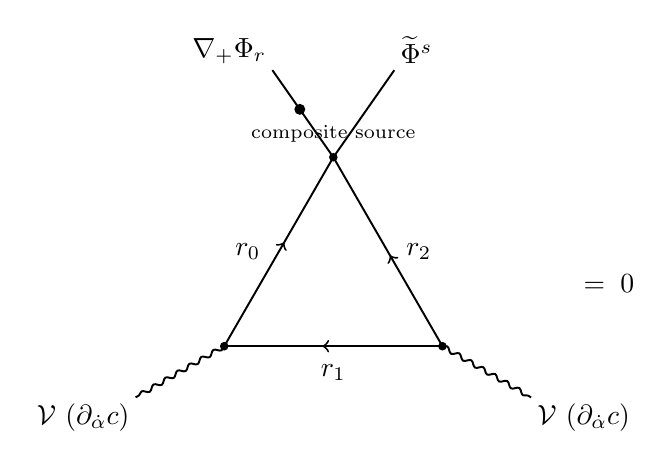
\begin{tikzpicture}
\coordinate (v0) at (90:1.6);
\coordinate (v1) at (210:1.6);
\coordinate (v2) at (330:1.6);
\node[svertex,label=above:{\scriptsize composite source}] at (v0) {};
\node[svertex] at (v1) {};
\node[svertex] at (v2) {};
\draw[sPhi] (v1) -- (v0) node[midway,left=3pt] {$r_{0}$};
\draw[sPhi] (v2) -- (v1) node[midway,below=3pt] {$r_{1}$};
\draw[sPhit] (v0) -- (v2) node[midway,right=3pt] {$r_{2}$};
\draw[sleg] (v0) -- ++(125:1.35) node[pos=0.55,sinsert]{}
  node[pos=1,above left=-2pt] {$\nabla_{+}\Phi_{r}$};
\draw[sleg] (v0) -- ++(55:1.35)
  node[pos=1,above right=-2pt] {$\widetilde\Phi^{s}$};
\draw[sV] (v1) -- ++(210:1.3)
  node[pos=1,below left=-2pt] {$\cV\ (\partial_{\dot\alpha}c)$};
\draw[sV] (v2) -- ++(330:1.3)
  node[pos=1,below right=-2pt] {$\cV\ (\partial_{\dot\alpha}c)$};
\node at (3.5,0) {$=\;0$};
\end{tikzpicture}
\caption{The representative ordinary matter-triangle parent of the
$(\beta_{r},\gamma^{s})$ family. The three edges are matter propagators with
edge momenta $r_{0},r_{1},r_{2}$, denominators $D_{i}=r_{i,d}^{2}$. The two
ordered sources sit at one composite-source vertex: the marked insertion
$\nabla_{+}\Phi_{r}$ (filled node) and the antichiral leg
$\widetilde\Phi^{s}$. The two output letters enter as the field-strength
preimages $\bcW_{\dot\alpha}^{(1)}=-\tfrac18\cD^{2}\bcD_{\dot\alpha}\cV$ on
the two vector legs at the two distinct remaining vertices (two distinct
superspace points). Every ordinary parent of the family vanishes on the
physical output word $\langle\partial c,\partial c\rangle$, as displayed;
the kernels themselves are nonzero
(Remark~\ref{rem:ss:bc:control}). The anomaly is instead the regulated
coincident Euler Jacobian of the kinetic
occurrence~\eqref{eq:ss:bc:kin}.}
\label{fig:ss:bc-triangle}
\end{figure}

\begin{remark}[Machine-zero verdict with nonzero-kernel control]%
\label{rem:ss:bc:control}
An external replay of the route census confirms the counts ($2+2$ routes for
$r=s$, $1+1$ for $r\neq s$, exactly one ordinary route able to carry the
two-$\partial c$ word) and the physical-word projection: every ordinary
parent --- all four $\partial c$-preimage assignments of the TMM triangles,
the evanescent residuals, the THH routes, the vector bridge, and the
nonlinear contact rows, in both orderings --- vanishes on
$\langle\partial c,\partial c\rangle$. The kernels themselves are nonzero: a
control evaluation of the same kernels on an off-physical test word returns a
nonzero value for both orderings, so the zeros are projections, not zero
kernels. Mechanically, two $\partial c$ letters cannot be saturated at a
single superspace point --- all same-point products of their preimages
vanish --- and the anomaly needs the two independent antichiral Fourier
variables of the coincident kernel of step 9.
\end{remark}

\paragraph{2. The kinetic source expansion and the order-$\cV^{2}$ orbit.}
The antichiral Euler operator was given in~\eqref{eq:ss:euler}:
\begin{equation}\label{eq:ss:bc:euler}
\frac{\delta S}{\delta\widetilde\Phi^{r}}
=-\frac14\,\nabla^{2}\Phi_{r}
-\frac{1}{\sqrt2}\,\varepsilon_{rtu}\,(\gamma^{t}\times\gamma^{u}) .
\end{equation}
Its kinetic piece is expanded covariantly \emph{before} any graph enumeration.
With the undotted frame index $a=(+,-)$, the gauge connection and its
expansion are
\begin{equation}\label{eq:ss:bc:gamma}
\Gamma_{a}:=e^{-\cV}\cD_{a}e^{\cV}
=\cD_{a}\cV+\frac12[\cD_{a}\cV,\cV]+O(\cV^{3}),
\qquad
\nabla_{a}=\cD_{a}+\Gamma_{a} ,
\end{equation}
and the graded Leibniz expansion on the even column $\Phi_{r}$ gives
\begin{equation}\label{eq:ss:bc:nablasq}
\begin{aligned}
\nabla^{2}\Phi_{r}
&=(\cD^{a}+\Gamma^{a})(\cD_{a}\Phi_{r}+\Gamma_{a}\Phi_{r})\\
&=\cD^{2}\Phi_{r}
+2\Gamma^{a}\cD_{a}\Phi_{r}
+(\cD^{a}\Gamma_{a})\Phi_{r}
+\Gamma^{a}\Gamma_{a}\Phi_{r} ,
\end{aligned}
\end{equation}
using $\Gamma_{a}\cD^{a}=-\Gamma^{a}\cD_{a}$. Therefore
$\tfrac12(\nabla^{2}\Phi_{r})\gamma^{s}
=\mathcal I_{0}+\mathcal I_{1}+\mathcal I_{2}+O(\cV^{3})$ with
\begin{align}
\mathcal I_{0}&=\frac12(\cD^{2}\Phi_{r})\gamma^{s} ,
\label{eq:ss:bc:I0}\\
\mathcal I_{1}&=\Big[(\cD^{a}\cV)\cD_{a}\Phi_{r}
+\frac12(\cD^{2}\cV)\Phi_{r}\Big]\gamma^{s} ,
\label{eq:ss:bc:I1}\\
\mathcal I_{2}&=\Big[
\frac12[\cD^{a}\cV,\cV]\cD_{a}\Phi_{r}
+\frac14\cD^{a}[\cD_{a}\cV,\cV]\Phi_{r}
+\frac12(\cD^{a}\cV)(\cD_{a}\cV)\Phi_{r}\Big]\gamma^{s} .
\label{eq:ss:bc:I2}
\end{align}
Writing $M_{1}$ and $M_{2}$ for the $\cV$ and $\cV^{2}/2$ terms of the
matter--gauge chain $\widetilde\Phi e^{\cV}\Phi$, the complete order-$\cV^{2}$
regulated orbit is the direct sum
\begin{equation}\label{eq:ss:bc:orbit}
\boxed{\;
\mathcal I_{0}\,\frac{1}{2!}M_{1}M_{1}
\;\oplus\;
\mathcal I_{1}M_{1}
\;\oplus\;
\mathcal I_{0}M_{2}
\;\oplus\;
\mathcal I_{2}\;}
\end{equation}
whose four rows are respectively the triangle parent, the nonlinear-source
collapsed contact, the matter seagull, and the source seagull. Their covariant
sum is the coincident kernel $K_{-}$ of step 9. The Schwinger source vector
field of step 4 has no vector, ghost, or non-minimal component, so there is no
gauge or ghost Jacobian orbit in this channel.

\paragraph{3. The three occurrence tags.}
The tree descendant of the unit-normalized insertion follows
from~\eqref{eq:ss:treeduction}:
\begin{equation}\label{eq:ss:bc:descendant}
\nabla_{-}(\nabla_{+}\Phi_{r})
=-2\,\frac{\delta S}{\delta\widetilde\Phi^{r}}
-\sqrt2\,\varepsilon_{rtu}\,(\gamma^{t}\times\gamma^{u}) .
\end{equation}
It must be expanded into three \emph{separately tagged occurrences}:
\begin{align}
\mathcal I_{E,\mathrm{kin}}^{AB}
&:=+\frac12(\nabla^{2}\Phi_{r})^{A}\,\gamma^{sB} ,
\label{eq:ss:bc:kin}\\
\mathcal I_{E,\mathrm{pot}}^{AB}
&:=+\sqrt2\,\varepsilon_{rtu}\,(\gamma^{t}\times\gamma^{u})^{A}\,\gamma^{sB} ,
\label{eq:ss:bc:epot}\\
\mathcal I_{X,\mathrm{pot}}^{AB}
&:=-\sqrt2\,\varepsilon_{rtu}\,(\gamma^{t}\times\gamma^{u})^{A}\,\gamma^{sB} ,
\label{eq:ss:bc:xpot}
\end{align}
the kinetic Euler occurrence (containing the inverse kinetic edge), the
Euler-potential occurrence, and the explicit-potential occurrence. The last
two rows have identical regulated contact kernels and opposite source
coefficients, and neither contains an inverse kinetic edge; they are retained
until their regulated evaluation pairs them in step 7. Replacing the tagged
descendant~\eqref{eq:ss:bc:descendant} by the single kinetic term
$\tfrac12\nabla^{2}\Phi_{r}$ before regulation erases the occurrence tags and
is not the computation performed here.

\begin{remark}[No contribution from the gauge-current orbit]%
\label{rem:ss:bc:gaugecurrent}
The vector equation of motion of~\eqref{eq:ss:euler} contains the current
$-2i(\Phi_{s}\times\widetilde\Phi^{s})$. Acting on it with $-\nabla_{+}$ and
using $\nabla_{+}\widetilde\Phi^{s}=0$ gives
$+2i\,(\nabla_{+}\Phi_{s}\times\widetilde\Phi^{s})$, which cancels the
explicit outer contact $-2i\,(\nabla_{+}\Phi_{s}\times\widetilde\Phi^{s})$
pointwise, for arbitrary independent external momenta, before any propagator
or loop integration; the gauge-fixing functional has only vector ports and
contributes nothing on this source. Hence no gauge-current or gauge-fixing
Jacobian feeds the $(\beta_r,\gamma^s)$ family: the entire anomaly is the
matter Euler Jacobian below.
\end{remark}

\paragraph{4. The Schwinger vector field and the surviving contraction.}
For the ordered source $(\beta_{r}^{A},\gamma^{sB})$ the Schwinger vector
field is the antichiral field redefinition
\begin{equation}\label{eq:ss:bc:X}
X_{rs}^{AB}(z)
:=\widetilde\Phi^{sB}(z)\,
\frac{\vec\delta}{\delta\widetilde\Phi^{rA}(z)} ,
\end{equation}
with support only on the integrated $\widetilde\Phi$ block: its vector,
Faddeev--Popov ghost, Nielsen--Kallosh and non-minimal components vanish
identically. The regulated Schwinger--Dyson identity of
Section~\ref{sec:superspace:sd} applied to $X_{rs}^{AB}$ gives
\begin{equation}\label{eq:ss:bc:sd}
0=\Big\langle
\operatorname{div}_{E,\epsilon}X_{rs}^{AB}
-\frac{1}{\h}\,X_{rs}^{AB}(S_{E})\Big\rangle,
\qquad
\Big\langle\gamma^{sB}\,
\Big(\frac{\delta S}{\delta\widetilde\Phi^{r}}\Big)^{A}\Big\rangle
=-\h g^{2}\,
\Big\langle\operatorname{div}_{E,\epsilon}X_{rs}^{AB}\Big\rangle ,
\end{equation}
the absorbed factor $g^{-2}$ of the frame of Section~\ref{sec:gaugebv} being
restored in this step only. The differentiated insertion fixes the flavor
tensor before any loop calculation:
\begin{equation}\label{eq:ss:bc:div}
\frac{\vec\delta\,\widetilde\Phi^{sB}(z)}{\delta\widetilde\Phi^{rA}(z)}
=\delta_{rs}\,\delta_{A}{}^{B}\,\delta_{-},
\qquad
\operatorname{div}_{E,\epsilon}X_{rs}^{AB}
=\delta_{rs}\,K_{-,\epsilon}^{AB}(z,z) ,
\end{equation}
with $\delta_{-}:=-\tfrac14\cD^{2}\delta_{e}$ the constrained coincident
antichiral delta and $K_{-,\epsilon}^{AB}(z,z)$ the coincident Euler-Jacobian
kernel. Thus $r\neq s$ vanishes independently of any external target. This
coincident self-contraction of the source pair is the only Wick contraction
surviving in the channel; at second order in the interaction the Dyson--Wick
weight is $\tfrac{1}{2!}(1+1)=1$, the two equivalent assignments of the two
interaction copies cancelling the $1/2!$.

\paragraph{5. The marked-edge $D$-algebra word.}
The marked linear source carries the exact edge word
\begin{equation}\label{eq:ss:bc:marked}
\mathcal M_{B}(r_{e})\,\delta_{e}
:=\cD_{-}\cD_{+}\bcD^{2}\cD^{2}\,\delta_{e}
=\frac12\,\cD^{2}\bcD^{2}\cD^{2}\,\delta_{e}
=8\,\bar r_{e}^{2}\,\cD^{2}\delta_{e} ,
\end{equation}
where the first equality uses $\cD_{-}\cD_{+}=\tfrac12\cD^{2}$ and the second
is the four-dimensional spinor $D$-algebra square of the edge momentum.
Dividing by the constrained matter-propagator factor $16D_{0}$,
$D_{0}:=r_{e,d}^{2}$,
\begin{equation}\label{eq:ss:bc:markedover}
\frac{\mathcal M_{B}(r_{e})\,\delta_{e}}{16D_{0}}
=\frac12\,\frac{\bar r_{e}^{2}}{D_{0}}\,\cD^{2}\delta_{e} .
\end{equation}
The full-$d$ Schwinger contact on the same edge is
$\tfrac12\big(r_{e,d}^{2}/D_{0}\big)\cD^{2}\delta_{e}$, and their difference
is
\begin{equation}\label{eq:ss:bc:markeddiff}
\frac12\,\frac{\mul^{2}}{D_{0}}\,\cD^{2}\delta_{e}
=-2\,\frac{\mul^{2}}{D_{0}}\,\delta_{-} .
\end{equation}
\begin{remark}[Two recorded conventions for the spinor-square identity]%
\label{rem:ss:bc:detsign}
The square $\cD^{2}\bcD^{2}\cD^{2}\delta^{4}=16\det(r)\,\cD^{2}\delta^{4}$ of
Section~\ref{sec:superspace:bb} (equation~\eqref{eq:ss:bb-projectorid}) and
the half square $8\,\bar r_{e}^{2}\,\cD^{2}\delta_{e}$
of~\eqref{eq:ss:bc:marked} are recorded with opposite signs relative to the
same determinant $\det r=-\bar r^{\,2}$. The two verification engines use
different superspace-derivative conventions --- one with real spinor
derivatives, the other with $i$-loaded ones, under which the operator square
scales by $i^{6}=-1$ --- and each machine-checks its own identity with its
recorded sign ($+16\det(r)$, respectively $-16\det(r)$, for the full square).
Each convention is used consistently within its own subsection, the physical
coefficients of both channels were machine-verified independently, and no
result is affected.
\end{remark}
The factor $2$ is the descendant factor of~\eqref{eq:ss:bc:descendant}; it is
not an additional graph multiplicity.

\paragraph{6. Cutting failure on the marked edge.}
On the selected Euler edge the four-dimensional square exceeds the
$d$-dimensional propagator inverse by the evanescent square,
$\bar r_{e}^{2}=r_{e,d}^{2}+\mul^{2}$. If the $D$-algebra square were the full
loop square, the Schwinger cut would be exact and the row would vanish:
\begin{equation}\label{eq:ss:bc:exactcut}
\frac{r_{e,d}^{2}}{D_{0}D_{1}D_{2}}-\frac{1}{D_{1}D_{2}}=0 .
\end{equation}
The spinor $D$-algebra supplies the four-dimensional square instead, so the
universal cutting-failure identity~\eqref{eq:ss:cuttingfailure} leaves only
\begin{equation}\label{eq:ss:bc:cutfail}
\frac{\bar r_{e}^{2}}{D_{0}D_{1}D_{2}}-\frac{1}{D_{1}D_{2}}
=\frac{\bar r_{e}^{2}-r_{e,d}^{2}}{D_{0}D_{1}D_{2}}
=\frac{\mul^{2}}{D_{0}D_{1}D_{2}} .
\end{equation}
Replacing $\bar r_{e}^{2}$ by $r_{e,d}^{2}$ before this subtraction makes the
expression identically zero and removes the anomaly.

\paragraph{7. The potential-row pairing.}
The two potential occurrences~\eqref{eq:ss:bc:epot} and~\eqref{eq:ss:bc:xpot}
carry no inverse kinetic edge; their regulated evaluations
$\mathcal R_{\epsilon}$ are ordinary contact rows built on one common kernel
$K_{\mathrm{pot}}$, and their opposite source coefficients pair them exactly:
\begin{equation}\label{eq:ss:bc:potpair}
\mathcal R_{\epsilon}\,\mathcal I_{E,\mathrm{pot}}^{AB}
+\mathcal R_{\epsilon}\,\mathcal I_{X,\mathrm{pot}}^{AB}
=\sqrt2\,K_{\mathrm{pot}}-\sqrt2\,K_{\mathrm{pot}}=0 .
\end{equation}
The kinetic Euler occurrence~\eqref{eq:ss:bc:kin} cannot be deleted with them:
it contains the inverse edge, and its Schwinger cut fails by exactly the
evanescent remainder~\eqref{eq:ss:bc:cutfail}.

\paragraph{8. The antichiral projector and the symbol trace.}
The external antichiral field strengths enter through the linearized preimage
\begin{equation}\label{eq:ss:bc:preimage}
\bcW_{\dot\alpha}^{(1)}=-\frac18\,\cD^{2}\bcD_{\dot\alpha}\cV ,
\end{equation}
and the locked antichiral projector of Section~\ref{sec:gaugebv}, normalized
per closed projector,
\begin{equation}\label{eq:ss:bc:projector}
\frac{1}{16}\,\nabla^{2}\bcD^{2}U
=\cD_{M}\cD^{M}U
-(\bcD_{\dot\beta}U)\,\bcW^{\dot\beta}
-\frac12\,U\,\nabla^{a}\cW_{a} ,
\end{equation}
($M$ the summed superspace derivative index of the locked projector)
contributes its $\bcW^{2}$ coefficient through exactly two copies of the
middle term, with squared coefficient $(-1)(-1)=+1$; the last term contains no
odd antichiral Fourier variable and cannot saturate the trace below. Let
$\bar\pi^{\dot1},\bar\pi^{\dot2}$ be the odd Fourier variables of the
antichiral delta and define the even symbol
\begin{equation}\label{eq:ss:bc:xi}
\Xi_{D}:=\bcW_{\dot\alpha}^{D}\,\bar\pi^{\dot\alpha}
=\bcW_{\dot1}^{D}\bar\pi^{\dot1}+\bcW_{\dot2}^{D}\bar\pi^{\dot2} .
\end{equation}
All four $\bcW$ and $\bar\pi$ generators are odd, so anticommuting them gives
\begin{equation}\label{eq:ss:bc:xixi}
\Xi_{D}\Xi_{E}
=\big(
\bcW_{\dot2}^{D}\bcW_{\dot1}^{E}
-\bcW_{\dot1}^{D}\bcW_{\dot2}^{E}
\big)\,\bar\pi^{\dot1}\bar\pi^{\dot2}
=\big\langle\bcW^{D},\bcW^{E}\big\rangle\,\bar\pi^{\dot1}\bar\pi^{\dot2} ,
\end{equation}
the dotted pairing of~\eqref{eq:ss:bilinear}. With the Berezin rule
$\int d\bar\pi^{\dot2}d\bar\pi^{\dot1}\,\bar\pi^{\dot1}\bar\pi^{\dot2}=1$, the
exact dotted trace is
\begin{equation}\label{eq:ss:bc:trace}
\boxed{\;\int d^{2}\bar\pi\;\Xi_{D}\Xi_{E}
=\big\langle\bcW^{D},\bcW^{E}\big\rangle .\;}
\end{equation}
For one color label,
$\Xi_{D}^{2}=\bcW^{D\dot\alpha}\bcW_{\dot\alpha}^{D}\,
\bar\pi^{\dot1}\bar\pi^{\dot2}$. The quadratic Dyson coefficient $1/2!$ and
the four-dimensional Gaussian
$\int\frac{d^{4}L}{(2\pi)^{4}}e^{-L^{2}/M^{2}}=\frac{M^{4}}{16\pi^{2}}$ fix
the coincident quadratic coefficient at
\begin{equation}\label{eq:ss:bc:gauss}
\frac{1}{2!}\cdot\frac{1}{M^{4}}\cdot\frac{M^{4}}{16\pi^{2}}
=\frac{1}{32\pi^{2}} ,
\end{equation}
the same normalization as the evanescent master
integral~\eqref{eq:ss:masterintegral}.

\paragraph{9. Color chains and the coincident kernel.}
For the ordered source $(\beta_{r}^{A},\gamma^{sB})$ the open adjoint chain of
the orbit is
\begin{equation}\label{eq:ss:bc:color}
(T_{D})^{A}{}_{Z}(T_{E})^{Z}{}_{C}\,\kappa^{CB}
=-f_{DZA}f_{EBZ}
=f_{AZD}f_{BZE}
=f^{ACD}f^{BCE} ,
\end{equation}
with the summed index relabeled in the last step. The independently routed
reverse source $(\gamma^{sA},\beta_{r}^{B})$ gives
\begin{equation}\label{eq:ss:bc:colorrev}
(T_{E})^{B}{}_{Z}(T_{D})^{Z}{}_{C}\,\kappa^{CA}
=-f_{EZB}f_{DAZ}
=f_{BZE}f_{AZD}
=f^{ACD}f^{BCE} ,
\end{equation}
the same ordered tensor. Since the dotted pairing of two odd letters is
symmetric (Section~\ref{sec:superspace:letters}), only the
$(D\!\leftrightarrow\!E)$-symmetric part of the color tensor contributes.
Combining the symbol trace~\eqref{eq:ss:bc:trace}, the color
chain~\eqref{eq:ss:bc:color}, the cutting failure~\eqref{eq:ss:bc:cutfail},
and the master value~\eqref{eq:ss:masterintegral}, the coincident kernel at
quadratic order in the antichiral field strength is
\begin{equation}\label{eq:ss:bc:kernel}
\boxed{\;
K_{-,\epsilon}^{AB}(z,z)\Big|_{\bcW^{2}}
=\frac{1}{32\pi^{2}}\,f^{ACD}f^{BCE}\,
\big\langle\bcW^{D},\bcW^{E}\big\rangle .\;}
\end{equation}

\paragraph{10. The evanescent master value and the tensor-integral pair.}
The triangle master integral of the channel is the universal
one~\eqref{eq:ss:masterintegral},
\begin{equation}\label{eq:ss:bc:master}
\lim_{\epsilon\to0}\mu^{2\epsilon}\!\int\!
\frac{d^{\,4-2\epsilon}L}{(2\pi)^{4-2\epsilon}}\,
\frac{\mul^{2}}{(L^{2}+\Delta)^{3}}
=\frac{1}{32\pi^{2}} ,
\end{equation}
independent of the Feynman-parameter combination $\Delta$, so the anomaly is a
polynomial in external momenta: a local operator. There is no graph-specific
factor $4-d$; the finite number is entirely the evanescent square multiplying
the logarithmic ultraviolet residue. Two further integrals belong to the
component cross-check of Section~\ref{sec:component}: with
$I_{n}(\Delta):=\int\frac{d^{d}\ell}{(2\pi)^{d}}\,
\mul^{2}/(\ell^{2}+\Delta)^{n}$ one has
$\lim_{\epsilon\to0}I_{3}(\Delta)=1/(32\pi^{2})$ and
$\lim_{\epsilon\to0}\Delta I_{4}(\Delta)=0$, and the rank-two box-type pair
\begin{equation}\label{eq:ss:bc:Jpair}
J:=\frac1d\int\frac{d^{d}\ell}{(2\pi)^{d}}\,
\frac{\mul^{2}\ell^{2}}{(\ell^{2}+\Delta)^{4}}
=\frac1d\big[I_{3}(\Delta)-\Delta I_{4}(\Delta)\big],
\qquad
\lim_{\epsilon\to0}J=\frac{1}{128\pi^{2}},
\qquad
\lim_{\epsilon\to0}2J=\frac{1}{64\pi^{2}} .
\end{equation}
The first number is the tensor integral; the second includes the explicit
factor $2$ of the four-dimensional sigma-matrix numerator. They cannot be
identified with each other, and neither is the triangle
master~\eqref{eq:ss:bc:master}: their role is to fix the free sign and the
loop-counting power (exactly one power of $\h$) of the component projection
quoted in step 13.

\paragraph{11. Final result.}
Since $\nabla_{-}\gamma^{s}=0$, only the descendant of the first letter acts.
Assembling the three occurrences, the Schwinger identity~\eqref{eq:ss:bc:sd},
the pairing~\eqref{eq:ss:bc:potpair}, and the kernel~\eqref{eq:ss:bc:kernel},
\begin{equation}\label{eq:ss:bc:assembly}
\begin{aligned}
\nabla_{-}\big((\nabla_{+}\Phi_{r})^{A}\gamma^{sB}\big)
\Big|_{\mathrm{1\text{-}loop}}
&=\Big\langle\Big[
-2\,\Big(\frac{\delta S}{\delta\widetilde\Phi^{r}}\Big)^{A}
-\sqrt2\,\varepsilon_{rtu}(\gamma^{t}\times\gamma^{u})^{A}
\Big]\gamma^{sB}\Big\rangle_{\!\mathrm{ev}}\\
&=\Big\langle
-2\,\Big(\frac{\delta S}{\delta\widetilde\Phi^{r}}\Big)^{A}
\Big|_{\mathrm{kin}}\gamma^{sB}\Big\rangle_{\!\mathrm{ev}}
+\big(\sqrt2\,K_{\mathrm{pot}}-\sqrt2\,K_{\mathrm{pot}}\big)\\
&=+2\,\delta_{rs}\,\h g^{2}\,
K_{-,\epsilon}^{AB}(z,z)\Big|_{\bcW^{2}}\\
&=2\,\delta_{rs}\,\h g^{2}\cdot\frac{1}{32\pi^{2}}\,
f^{ACD}f^{BCE}\,\big\langle\bcW^{D},\bcW^{E}\big\rangle\\
&=\delta_{rs}\,\frac{\h g^{2}}{16\pi^{2}}\,
f^{ACD}f^{BCE}\,\big\langle\bcW^{D},\bcW^{E}\big\rangle .
\end{aligned}
\end{equation}
The normalization trace is: Schwinger descendant $(-2)(-\h g^{2})=+2\h g^{2}$;
coincident kernel $\tfrac{1}{2!}\cdot\tfrac{1}{16\pi^{2}}=\tfrac{1}{32\pi^{2}}$;
product $2\h g^{2}/(32\pi^{2})=\h g^{2}/(16\pi^{2})$ --- exactly one power of
$\h$, the universal one-loop coefficient. Restoring the letter normalization,
$\beta_{r}=\tfrac{1}{\sqrt2}\nabla_{+}\Phi_{r}$ absorbs one factor $\sqrt2$,
and $\partial_{\dot\alpha}c=i\bcW_{\dot\alpha}$ contributes $i^{2}=-1$ to the
dotted pairing, so
\begin{equation}\label{eq:ss:bc:result}
\boxed{\;
\nabla_{-}\big(\beta_{r}^{A}\gamma^{sB}\big),\quad
\nabla_{-}\big(\gamma^{sA}\beta_{r}^{B}\big)
=-\frac{\h g^{2}}{16\sqrt2\,\pi^{2}}\,f^{ACD}f^{BCE}\,
\delta_{rs}\,\langle\partial c,\partial c\rangle^{DE} ,\;}
\end{equation}
exactly the row~\eqref{eq:ss:ch-betagamma} of the channel table. The two
orderings are equal and independent: $|\gamma^{s}|=0$ and
$\nabla_{-}\gamma^{s}=0$ give
$\nabla_{-}(\gamma^{sA}\beta_{r}^{B})=\gamma^{sA}\nabla_{-}\beta_{r}^{B}$, and
the independent reverse Schwinger vector field with the reverse color
chain~\eqref{eq:ss:bc:colorrev} produces the same ordered tensor. The twelve
flavor-off-diagonal pairs, $r\neq s$, are exact zeros by the $\delta_{rs}$
of~\eqref{eq:ss:bc:div} --- the singlet contraction
$\delta_{rs}\langle\partial c,\partial c\rangle$ has no off-diagonal support,
census class (ii) of Section~\ref{sec:superspace:selection}.

\begin{remark}[Where the ordinary-parent obstruction applies, and where it
does not]\label{rem:ss:bc:olderror}
The ordinary bottom-component census remains correct on its own terrain: the
mixed quadratic blocks vanish,
$G_{\phi\widetilde\psi}=G_{\psi\widetilde\phi}=0$, so no ordinary component
triangle with two external-$\partial c$ Yukawa vertices and the bottom sources
exists. That statement does not evaluate the Schwinger occurrence. The
occurrence first differentiates the coincident insertion,
$\widetilde\Phi^{sB}\vec\delta/\delta\widetilde\Phi^{rA}
\to\delta_{rs}K_{-,\epsilon}^{AB}(z,z)$, and only then admits a bottom
projection; promoting the ordinary-parent obstruction to a statement about the
regulated density divergence is rejected. The order of operations in this
subsection --- occurrence tags, Schwinger--Dyson identity, regulated pairing,
coincident kernel --- is the accepted one; an external audit of the full
family passes all $84$ of its checks, and the physical verifier passes all
$33$ of its sector checks.
\end{remark}

\paragraph{12. Holomorphic-twist comparison and the generalized Konishi
anomaly.}
The holomorphic-twist computation of \cite{BK} prints, for this family (their
eq.~(3.65)),
\begin{equation}\label{eq:ss:bc:bk}
Q_{1}\big((\beta_{I})^{A}(\gamma^{J})^{B}\big)
=\kappa_{H}^{2}\,\delta^{J}_{I}\,f_{ACD}f_{BCE}\,
\partial_{\dot\alpha}c^{D}\,\partial^{\dot\alpha}c^{E} .
\end{equation}
With the loop-scale identification
$\hbar_{\mathrm{HT}}\kappa_{H}^{2}=\h g^{2}/(32\sqrt2\,\pi^{2})$ of
Section~\ref{sec:ht}, the twist prefactor $-2\kappa_{H}^{2}\hbar_{\mathrm{HT}}$
is exactly the uniform prefactor $-\h g^{2}/(16\sqrt2\,\pi^{2})$
of~\eqref{eq:ss:bc:result}, and the output words agree for both orderings ---
only $(\beta,\gamma)$ is printed in \cite{BK}; $(\gamma,\beta)$ follows from
supercommutative normal ordering with no sign --- and for all off-diagonal
pairs, which vanish on both sides. Physically, the $(\beta_r,\gamma^s)$
channel \emph{is} the regulated generalized Konishi anomaly: the density
divergence of the functional measure under the antichiral source
redefinition~\eqref{eq:ss:bc:X}. The full eighty-one-channel table is its
completion over the BPS letter alphabet, obtained here by a direct superspace
supergraph computation with no twist-formalism input.

\begin{remark}[Status of the comparison]\label{rem:ss:bc:htstatus}
The loop-scale identification is a conditional dictionary entry, not a theorem
of this paper; the comparison is performed on output words, and it is a
cross-check, not an internal completeness proof of the graph census. The
Konishi identification is stated at the level of the mechanism --- the
regulated density divergence of the measure; an independent re-derivation of
the classic generalized-Konishi formula in the present conventions is not
claimed: the channel computation itself is the derivation offered. The full
dictionary, the derivative-tower kernel, and the factor-two adjudication are
in Section~\ref{sec:ht}.
\end{remark}

\paragraph{13. Component bottom-projection cross-check.}
The bottom components of the letters are $\beta_{r}|=\psi_{r+}$,
$\gamma^{s}|=\widetilde\phi^{s}$,
$\partial_{\dot\alpha}c|=-\widetilde\lambda_{\dot\alpha}$
(Section~\ref{sec:component}), so at zero extra holomorphic derivative
$\langle\partial c,\partial c\rangle^{DE}\big|
=\widetilde\lambda_{\dot\alpha}^{D}\widetilde\lambda^{E\dot\alpha}$, and the
left-hand side of~\eqref{eq:ss:bc:result} projects to
$Q_{-}(\psi_{r+}^{A}\widetilde\phi_{s}^{B})$. The bottom projection of the
superfield result is therefore
\begin{equation}\label{eq:ss:bc:component}
Q_{-}\!\left(\psi_{r+}^{A}\widetilde\phi_{s}^{B}\right)
\Big|_{\mathrm{1\text{-}loop}}
=-\frac{\sqrt2\,\h g^{2}}{32\pi^{2}}\,
\delta_{rs}\,f^{ACD}f^{BCE}\,
\widetilde\lambda_{\dot\alpha}^{D}\widetilde\lambda^{E\dot\alpha} ,
\end{equation}
using $1/(16\sqrt2)=\sqrt2/32$. This is an exact projection
of~\eqref{eq:ss:bc:result}, not an independent component-box derivation: the
mixed propagators vanish, so no ordinary two-Yukawa parent exists at the
component level, and the dotted gaugino bilinear is color-symmetric,
$\widetilde\lambda_{\dot\alpha}^{D}\widetilde\lambda^{E\dot\alpha}
=\widetilde\lambda_{\dot\alpha}^{E}\widetilde\lambda^{D\dot\alpha}$, so any
antisymmetric color word would annihilate it. The full component treatment,
including the role of the tensor pair~\eqref{eq:ss:bc:Jpair}, is in
Section~\ref{sec:component}.

\subsection{The complete channel table}\label{sec:superspace:table}

We now state all seven nonzero families of the master
identity~\eqref{eq:ss:master}. The letter
definitions~\eqref{eq:ss:letters} induce a uniform rescaling between the
unit-normalized field-strength composites used in the graph computations and
the letters of Definition~\ref{def:ss:letters}. The bookkeeping is immediate:
in the seed channel the two insertions contribute $(-i/\sqrt2)^2=-\tfrac12$
and the output bilinears contribute $\sqrt2$, giving the net prefactor
$-\tfrac12\cdot\sqrt2\cdot\tfrac{\h g^2}{16\pi^2}
=-\tfrac{\h g^{2}}{16\sqrt2\,\pi^{2}}$ of equation~\eqref{eq:ss:bbresult}.
The same arithmetic, applied family by family, yields the common prefactor
$-\h g^{2}/(16\sqrt2\,\pi^{2})$ for every family, including the
$(b,\beta)/(\beta,b)$ family, whose output word is fixed by the
residual-supersymmetry closure discussed below.
With $\langle X,Y\rangle$ as in~\eqref{eq:ss:bilinear} and
$\partial_{\dot\alpha}(\partial c)$ the holomorphic derivative of the letter
$\partial c$, the complete set of nonzero channels is
\begin{align}
\nabla_{-}\big(b^{A}b^{B}\big)
&=-\frac{\h g^{2}}{16\sqrt2\,\pi^{2}}\,f^{ACD}f^{BCE}\,
\Big\{\langle\partial c,b\rangle-\langle b,\partial c\rangle
+\textstyle\sum_r\big(\langle\beta_r,\gamma^r\rangle
-\langle\gamma^r,\beta_r\rangle\big)\Big\}^{DE},
\label{eq:ss:ch-bb}\\[4pt]
\nabla_{-}\big(b^{A}\gamma^{rB}\big),\quad
\nabla_{-}\big(\gamma^{rA}b^{B}\big)
&=-\frac{\h g^{2}}{16\sqrt2\,\pi^{2}}\,f^{ACD}f^{BCE}\,
\big\{\langle\partial c,\gamma^{r}\rangle
-\langle\gamma^{r},\partial c\rangle\big\}^{DE},
\label{eq:ss:ch-bgamma}\\[4pt]
\nabla_{-}\big(\beta_{r}^{A}\gamma^{sB}\big),\quad
\nabla_{-}\big(\gamma^{sA}\beta_{r}^{B}\big)
&=-\frac{\h g^{2}}{16\sqrt2\,\pi^{2}}\,f^{ACD}f^{BCE}\,
\delta_{rs}\,\langle\partial c,\partial c\rangle^{DE},
\label{eq:ss:ch-betagamma}\\[4pt]
\nabla_{-}\big(\beta_{r}^{A}\beta_{s}^{B}\big)
&=-\frac{\h g^{2}}{16\sqrt2\,\pi^{2}}\,f^{ACD}f^{BCE}\,
\varepsilon_{rst}\,
\big\{\langle\partial c,\gamma^{t}\rangle
-\langle\gamma^{t},\partial c\rangle\big\}^{DE},
\label{eq:ss:ch-betabeta}\\[4pt]
\nabla_{-}\big(b^{A}\beta_{r}^{B}\big),\quad
\nabla_{-}\big(\beta_{r}^{A}b^{B}\big)
&=-\frac{\h g^{2}}{16\sqrt2\,\pi^{2}}\,f^{ACD}f^{BCE}\,
\big\{\langle\beta_{r},\partial c\rangle
+\langle\partial c,\beta_{r}\rangle
+\varepsilon_{rst}\langle\gamma^{s},\gamma^{t}\rangle\big\}^{DE},
\label{eq:ss:ch-bbeta}\\[4pt]
\nabla_{-}\big(b^{A}\partial_{\dot\alpha}c^{B}\big)
&=-\frac{\h g^{2}}{16\sqrt2\,\pi^{2}}\,f^{ACD}f^{BCE}\,
\Big\{\tfrac13\big\langle\partial_{\dot\alpha}(\partial c),\partial c\big\rangle
+\tfrac23\big\langle\partial c,\partial_{\dot\alpha}(\partial c)\big\rangle
\Big\}^{DE},
\label{eq:ss:ch-bdc}\\[4pt]
\nabla_{-}\big(\partial_{\dot\alpha}c^{A}b^{B}\big)
&=-\frac{\h g^{2}}{16\sqrt2\,\pi^{2}}\,f^{ACD}f^{BCE}\,
\Big\{\tfrac23\big\langle\partial_{\dot\alpha}(\partial c),\partial c\big\rangle
+\tfrac13\big\langle\partial c,\partial_{\dot\alpha}(\partial c)\big\rangle
\Big\}^{DE}.
\label{eq:ss:ch-dcb}
\end{align}
The free dotted index in~\eqref{eq:ss:ch-bdc} and~\eqref{eq:ss:ch-dcb} is the
letter index of $\partial_{\dot\alpha}c$ on the left and the extra holomorphic
derivative on the right; the weights $(\tfrac13,\tfrac23)$ are the
$(m,n)=(1,0)$ instance of the tower kernel of
Section~\ref{sec:superspace:tower}. Together with the fifty-two zeros of
Section~\ref{sec:superspace:selection}, the rows
\eqref{eq:ss:ch-bb}--\eqref{eq:ss:ch-dcb} exhaust the eighty-one ordered
channels: $1+6+6+4+6+6=29$ nonzero, as in~\eqref{eq:ss:29}.

\subsubsection*{Residual-supersymmetry closure of the $(b,\beta)/(\beta,b)$
channels}

The family~\eqref{eq:ss:ch-bbeta} is the only one whose output word is not
read off a cut parent graph directly. The raw graph carrier of this family
contains an equation-of-motion (total-derivative) layer; the physical answer
is the unique residual-supersymmetry-closed vector obtained after removing
that layer and adding a finite normal-product (scheme) term, with the
remaining one-parameter freedom anchored to the $(b,b)$ scale. The closure
works as follows. The residual supercharges of the bottom-letter sector,
$q_r:=\tfrac{1}{\sqrt2}Q^{r}_{E,+}$, act on the letters by
\begin{equation}\label{eq:ss:qaction}
q_r\,b=0,
\qquad
q_r\,\beta_s=\delta_{rs}\,b,
\qquad
q_r\,\gamma^{s}=-\varepsilon_{rst}\,\beta_t,
\qquad
q_r\,(\partial_{\dot\alpha}c)=\partial_{\dot\alpha}\gamma^{r} .
\end{equation}
At twisted dimension $\tfrac92$, the space of odd $SU(3)$-singlet letter
bilinears annihilated by all $q_r$ is one-dimensional, spanned by the seed
output word
\begin{equation}\label{eq:ss:singlet}
\big\{\langle\partial c,b\rangle-\langle b,\partial c\rangle
+\textstyle\sum_r\big(\langle\beta_r,\gamma^r\rangle
-\langle\gamma^r,\beta_r\rangle\big)\big\}^{DE}
\end{equation}
of~\eqref{eq:ss:ch-bb}. The $(b,\beta_r)$ output word is its unique triplet
$q$-primitive:
\begin{equation}\label{eq:ss:triplet}
q_s\big\{\langle\beta_r,\partial c\rangle+\langle\partial c,\beta_r\rangle
+\varepsilon_{rtu}\langle\gamma^{t},\gamma^{u}\rangle\big\}
=-\delta_{sr}\,
\Big\{\langle\partial c,b\rangle-\langle b,\partial c\rangle
+\textstyle\sum_{r'}\big(\langle\beta_{r'},\gamma^{r'}\rangle
-\langle\gamma^{r'},\beta_{r'}\rangle\big)\Big\} .
\end{equation}
Equivalently, in the ordered basis
$\big(\langle\partial c,\beta_r\rangle,\,\langle\beta_r,\partial c\rangle,\,
\langle\gamma^{s},\gamma^{t}\rangle,\,\langle\gamma^{t},\gamma^{s}\rangle\big)$
with $\varepsilon_{rst}=+1$, the three Ward equations $q_s[\,\cdot\,]=0$
($s=1,2,3$) cut out the one-dimensional ray spanned by $(1,1,1,-1)$, and
anchoring this ray to the $(b,b)$ scale through~\eqref{eq:ss:triplet} fixes
the unit normalization displayed in~\eqref{eq:ss:ch-bbeta}. Since
$q_r(b^Ab^B)=0$, the seed channel's own forward orbit is only itself: the
physical families were each computed directly, and the closure is a
cross-check that fixes the $(b,\beta)$ normalization.

\begin{remark}[The finite shift is a scheme term, not an anomaly graph]%
\label{rem:ss:finiteshift}
The passage from the raw graph carrier to the renormalized coefficient vector
of the $(b,\beta)/(\beta,b)$ family removes an equation-of-motion
(total-derivative) layer and adds a finite normal-product term. This is a
finite scheme adjustment, not an additional anomaly graph: all bare-graph
anomaly in every channel comes only from the $\mul^{2}$ cutting
failure~\eqref{eq:ss:cuttingfailure}. The closure was verified by thirty-one
independent finite Ward-identity checks. Through this finite shift and the
anchoring to the $(b,b)$ scale, the $(b,\beta)/(\beta,b)$ family lands on the
same universal prefactor $-\h g^{2}/(16\sqrt2\,\pi^{2})$ as every other
nonzero family, with the output word displayed in~\eqref{eq:ss:ch-bbeta}.
\end{remark}

\subsection{The holomorphic-derivative tower}\label{sec:superspace:tower}

Shifting the second letter of a channel bilinear by a formal vector $w$ ---
equivalently, resumming all holomorphic derivatives --- inserts the leg phase
$e^{iw\cdot(aq+bp)}$ into the ordered Feynman parametrization of the triangle.
The ordered-simplex moment is
\begin{equation}\label{eq:ss:simplexmoment}
\int_{0<a<b<1}a^{p}b^{q}\,da\,db=\frac{1}{(p+1)(p+q+2)} ,
\end{equation}
so that
\begin{equation}\label{eq:ss:simplexderivation}
2\int_{0}^{1}\!db\int_{0}^{b}\!da\;a^{k+\ell}\,b^{(m-k)+(n-\ell)}
=\frac{2}{(k+\ell+1)(m+n+2)} .
\end{equation}
Restoring the binomial weights of the derivative expansion gives the one-loop
holomorphic-derivative kernel
\begin{equation}\label{eq:ss:kernel}
\boxed{\;
K_{m,n;k,\ell}
=\frac{2\binom{m}{k}\binom{n}{\ell}}{(m+n+2)(k+\ell+1)}\;}
\qquad
(m,n\in\mathbb Z_{\geq0},\ 0\leq k\leq m,\ 0\leq\ell\leq n).
\end{equation}

\begin{remark}[The overall factor $2$ is $\Gamma(3)$]\label{rem:ss:gamma3}
The numerator factor $2$ in~\eqref{eq:ss:kernel} is
$\Gamma(3)$ from combining the three denominators,
$\frac{1}{D_0D_1D_2}=2\int_{\Delta_2}\frac{1}{(r^{2}+\Delta)^{3}}$; it is not
an orientation multiplicity and not a second loop orientation.
\end{remark}

Because the $\partial_{\dot\alpha}$ are gauge-covariant and do not commute,
derivative monomials are understood as shuffle-symmetrized averages over the
$(m,n)$ orderings of $\partial_{\dot1}^{m}\partial_{\dot2}^{n}$. The full
kernel operator on letter pairs is
\begin{equation}\label{eq:ss:kerneloperator}
\mathcal K_{m,n}(f^{D},g^{E})
=\sum_{k=0}^{m}\sum_{\ell=0}^{n}
\frac{2\binom{m}{k}\binom{n}{\ell}}{(m+n+2)(k+\ell+1)}\,
\big(\partial_{\dot1}^{k}\partial_{\dot2}^{\ell}\partial_{\dot\alpha}f\big)^{D}
\big(\partial_{\dot1}^{\,m-k}\partial_{\dot2}^{\,n-\ell}
\partial^{\dot\alpha}g\big)^{E} .
\end{equation}
Its first instances are
\begin{align}
\mathcal K_{0,0}&=\langle f,g\rangle,
\qquad
\mathcal K_{1,0}=\frac13\langle\partial_{\dot1}f,g\rangle
+\frac23\langle f,\partial_{\dot1}g\rangle,
\label{eq:ss:kernelexamples1}\\
\mathcal K_{2,0}&=\frac16\langle\partial_{\dot1}^{2}f,g\rangle
+\frac12\langle\partial_{\dot1}f,\partial_{\dot1}g\rangle
+\frac12\langle f,\partial_{\dot1}^{2}g\rangle,
\label{eq:ss:kernelexamples2}\\
\mathcal K_{1,1}&=\frac16\langle\partial_{\dot1}\partial_{\dot2}f,g\rangle
+\frac14\langle\partial_{\dot1}f,\partial_{\dot2}g\rangle
+\frac14\langle\partial_{\dot2}f,\partial_{\dot1}g\rangle
+\frac12\langle f,\partial_{\dot1}\partial_{\dot2}g\rangle .
\label{eq:ss:kernelexamples3}
\end{align}
In particular the $(b,\partial c)$ weights $(\tfrac13,\tfrac23)$ of
\eqref{eq:ss:ch-bdc}--\eqref{eq:ss:ch-dcb} are the $(m,n)=(1,0)$ instance:
$K_{1,0;1,0}=\tfrac{2}{3\cdot2}=\tfrac13$ for the derivative on the first
letter and $K_{1,0;0,0}=\tfrac{2}{3\cdot1}=\tfrac23$ for the derivative on
the second. The comparison of~\eqref{eq:ss:kernel} with the holomorphic-twist
kernel of \cite{BK} is the subject of Section~\ref{sec:ht}.

% sec05-component.tex -- pure body LaTeX; shared macros from main.tex only.
\section{The component Feynman-diagram approach}\label{sec:component}

\subsection{The program: component quantization of the same action}%
\label{sec:component:program}

The one-loop anomalous supersymmetry Ward identity of this paper was derived in
Euclidean $\mathcal N=1$ superspace (Section~\ref{sec:superspace}). The present
section develops the parallel component-field approach: the same Euclidean
action of Sections~\ref{sec:notation} and \ref{sec:gaugebv}, expanded in
component fields and quantized by ordinary Feynman diagrams. An independent
component check is desirable for three reasons: the component expansion makes
the anomaly directly readable as a bottom-component transformation law; the
off-shell formulation carries an off-shell Noether current for the
supersymmetry, in whose divergence the anomaly would appear as an
Euler-operator insertion, checkable term by term \cite{WeinbergIII,GGRS}; and
ordinary Wick diagrams, regulable by dimensional reduction \cite{SiegelDRED},
give a graph-by-graph cross-check of the superspace Schwinger--Dyson
derivation, with no superspace $D$-algebra anywhere in the loop evaluation.

The component content of the theory is the $\mathcal N=1$ vector multiplet
$(A_m,\lambda,D)$ together with three adjoint chiral multiplets
$(\phi_r,\psi_r,F_r)$, $r=1,2,3$, and their independent Euclidean antichiral
partners $(\widetilde\phi_r,\widetilde\psi_r,\widetilde F_r)$ and
$\widetilde\lambda$: tilded and untilded fields are independent integration
variables in Euclidean signature and become Lorentzian conjugates only after a
real integration cycle is selected. With the color commutator
$[X,Y]^A:=f^{BCA}X^BY^C$ and $\kappa_{AB}=\delta_{AB}$
(Section~\ref{sec:notation}), the exact Euclidean off-shell $\mathcal N=4$
component Lagrangian is
\begin{equation}\label{eq:05:offshell}
\boxed{
\begin{aligned}
\mathcal L_{E,\mathrm{off}}^{(4)}={}&
\frac{1}{g^{2}}\delta_{AB}\Big[
\frac14 F_{mn}^{A}F_{mn}^{B}
+\widetilde\lambda^{A}\bar\sigma_E^{m}\mathcal D_m\lambda^{B}
-\frac12 D^{A}D^{B}
+(\mathcal D_m\widetilde\phi_r)^{A}(\mathcal D_m\phi_r)^{B}
+\widetilde\psi_r^{A}\bar\sigma_E^{m}\mathcal D_m\psi_r^{B}
-\widetilde F_r^{A}F_r^{B}
-iD^{A}[\phi_r,\widetilde\phi_r]^{B}\Big]\\
&-\frac{\sqrt2}{g^{2}}f^{ABC}
\big(\widetilde\phi_r^{A}\psi_r^{B}\lambda^{C}
+\phi_r^{A}\widetilde\psi_r^{B}\widetilde\lambda^{C}\big)
+\frac{1}{\sqrt2\,g^{2}}\varepsilon_{rst}f^{ABC}
\big(F_r^{A}\phi_s^{B}\phi_t^{C}
+\widetilde F_r^{A}\widetilde\phi_s^{B}\widetilde\phi_t^{C}
-\phi_t^{A}\psi_r^{B}\psi_s^{C}
-\widetilde\phi_t^{A}\widetilde\psi_r^{B}\widetilde\psi_s^{C}\big),
\end{aligned}}
\end{equation}
plus a topological term that plays no role below and is omitted from the
display. Here $D^A$ is the vector-multiplet auxiliary scalar (not a
derivative), $\bar\sigma_E^m$ are the Euclidean sigma matrices, and repeated
flavor indices are summed. Eliminating the auxiliaries through
$D=-i[\phi_r,\widetilde\phi_r]$,
$\widetilde F_r=\tfrac{1}{\sqrt2}\varepsilon_{rst}[\phi_s,\phi_t]$,
$F_r=\tfrac{1}{\sqrt2}\varepsilon_{rst}[\widetilde\phi_s,\widetilde\phi_t]$
gives the on-shell component action. The two Yukawa families
$-\frac{\sqrt2}{g^2}f^{ABC}\widetilde\phi_r^A\psi_r^B\lambda^C$ and
$-\frac{\sqrt2}{g^2}f^{ABC}\phi_r^A\widetilde\psi_r^B\widetilde\lambda^C$
in \eqref{eq:05:offshell} are the only vertices carrying the fields of the
anomaly; they are the vertices from which a naive ordinary component
derivation would have to be built (Section~\ref{sec:component:accepted}).

The component framework also locks the BV--BRST structure exactly. With chiral
and antichiral Faddeev--Popov ghost superfields $c$ and $\widetilde c$, both of
ghost number $+1$, the BRST differential acts on the unrestricted vector
prepotential $\cV$ and the matter superfields as
\begin{equation}\label{eq:05:brst}
\boxed{
s\,e^{\cV}=i\widetilde c\,e^{\cV}-i e^{\cV}c,\quad
s\,c=ic^{2},\quad
s\,\widetilde c=i\widetilde c^{\,2},\quad
s\,\Phi_r=ic\,\Phi_r,\quad
s\,\widetilde\Phi_r=-i\widetilde\Phi_r\,\widetilde c.}
\end{equation}
This differential is nilpotent, $s^2=0$. The minimal Batalin--Vilkovisky action
obeys the classical master equation and, after the finite-cutoff regulator
insertion, the order-by-order quantum master equation \cite{BV}. Gauge fixing
uses a nonminimal sector with the antighost $\bar c$ and the gauge functions
$\mathcal F_\pm(\cV)=-\tfrac14\bcD^{2}\cV,\,-\tfrac14\cD^{2}\cV$;
the Wess--Zumino surface is not imposed before gauge fixing.

\begin{remark}[Partial scope of the component Feynman rules]%
\label{rem:05:partialscope}
Locked exactly are the component actions, the BV--BRST structure, and the
all-order primitive graph grammar with labeled-graph weights; this grammar
becomes a numerical Feynman rule only after every edge inverse and integration
cycle is locked. The Fermi--Feynman gauge-averaged propagators exist only
conditionally: the corresponding gauge-fixing kernel contains $\BoxE^{-1}$ and
is nonlocal, so an admissible completed perturbative slice is not claimed
(status \texttt{PASS\_EXACT\_PARTIAL\_SCOPE}). The accepted superspace
computation of Section~\ref{sec:superspace} therefore adopts the
Fermi--Feynman Gaussian average as a recorded scheme decision and keeps the
Nielsen--Kallosh factor as an external, field-independent measure. Former
claims of complete component momentum-space Feynman rules are
\texttt{NOT\_ACCEPTED\_COMPLETE\_FEYNMAN\_RULES}.
\end{remark}

This component approach is one of four mutually independent computations into
which the proof program is organized: signature (Euclidean or Lorentzian) times
formulation (superspace or component). Each works from the shared frozen
conventions and its own derivations only, and results are compared only at the
final canonical level. Gating rules order them: the Euclidean component
computation begins once the conventions are frozen, the Euclidean superspace
one starts after the Euclidean component canonical result is locked, and the
two Lorentzian ones start only after a Euclidean bridge is frozen. The accepted
component statement below is in fact obtained as the bottom projection of the
Euclidean superspace result---explicitly not as an independent component-box
derivation.

\subsection{The accepted result: bottom projection of the
\texorpdfstring{$(\beta,\gamma)$}{(beta,gamma)} anomaly}%
\label{sec:component:accepted}

Section~\ref{sec:superspace} establishes, for the ordered letter pair
$(\beta_r,\gamma^s)$ and equally for the reversed ordering
$(\gamma^s,\beta_r)$, the exact one-loop identity
\begin{equation}\label{eq:05:superfieldBC}
\nabla_-\!\big(\beta_r^{A}\gamma^{sB}\big)\Big|_{\text{1-loop}}
=-\frac{\h g^{2}}{16\sqrt2\,\pi^{2}}\,\delta_{rs}\,f^{ACD}f^{BCE}\,
\langle\partial c^{D},\partial c^{E}\rangle ,
\end{equation}
where $\langle X,Y\rangle:=(\partial_{\dot\alpha}X)(\partial^{\dot\alpha}Y)$
is the dotted pairing and $\nabla_-$ is the anomalous frame component of the
gauge-covariant spinor derivative. Its component content is read off by bottom
projection. The bottom components of the letters are
\begin{equation}\label{eq:05:bottomproj}
\beta_r^{A}\big|=\psi_{r+}^{A},
\qquad
\gamma^{sB}\big|=\widetilde\phi_s^{B},
\qquad
\partial_{\dot\alpha}c^{D}\big|=-\widetilde\lambda_{\dot\alpha}^{D},
\end{equation}
where $\psi_{r+}$ is the $+$-frame bottom component of the $r$-th matter Weyl
fermion, $\widetilde\phi_s$ the bottom scalar of the antichiral multiplet, and
$\widetilde\lambda$ the dotted gaugino. The component variation $Q_-$ is the
bottom action induced by the same locked $\nabla_-$ acting on the letters; no
independent rephasing is introduced. The dotted pairing projects as
\begin{equation}\label{eq:05:pairingproj}
\langle\partial c^{D},\partial c^{E}\rangle\Big|
=\big(\partial_{\dot\alpha}c^{D}\big)\big(\partial^{\dot\alpha}c^{E}\big)\Big|
=\widetilde\lambda_{\dot\alpha}^{D}\widetilde\lambda^{E\dot\alpha}.
\end{equation}
Combining \eqref{eq:05:superfieldBC}--\eqref{eq:05:pairingproj} gives the
accepted component formula
\begin{equation}\label{eq:05:bccomponent}
\boxed{
Q_-\!\left(\psi_{r+}^{A}\widetilde\phi_s^{B}\right)\Big|_{\text{1-loop}}
=-\frac{\sqrt2\,\h g^{2}}{32\pi^{2}}\,\delta_{rs}\,f^{ACD}f^{BCE}\,
\widetilde\lambda_{\dot\alpha}^{D}\widetilde\lambda^{E\dot\alpha}.}
\end{equation}

\begin{remark}[Status of the boxed formula]\label{rem:05:status}
Equation \eqref{eq:05:bccomponent} is an exact projection of the accepted
superfield result of Section~\ref{sec:superspace}, not an independent
component-box derivation. It fixes the former free sign of the component-box
proposal to $-1$, and the loop order contains exactly one power of $\h$.
\end{remark}

The dotted gaugino bilinear on the right of \eqref{eq:05:bccomponent} has a
color symmetry that constrains every component realization. With
$\epsilon^{\dot1\dot2}=+1$, define
\begin{equation}\label{eq:05:gauginoS}
S^{DE}:=\widetilde\lambda_{\dot\alpha}^{D}\widetilde\lambda^{E\dot\alpha}
=\widetilde\lambda_{\dot1}^{D}\widetilde\lambda_{\dot2}^{E}
-\widetilde\lambda_{\dot2}^{D}\widetilde\lambda_{\dot1}^{E},
\qquad S^{ED}=S^{DE},
\end{equation}
where the second relation is Grassmann reordering. Consequently, any
antisymmetric color coefficient $A_{DE}=-A_{ED}$ obeys
\begin{equation}\label{eq:05:antisymm}
A_{DE}S^{DE}=\frac12\big(A_{DE}+A_{ED}\big)S^{DE}=0:
\end{equation}
antisymmetric color words vanish, the former crossed word $W_{DE}-W_{ED}$
gives zero, and a nonzero result for the ordered pair $(\beta,\gamma)$ must
carry the symmetric color projection $f^{ACD}f^{BCE}S^{DE}$, which is indeed
symmetric in $D\leftrightarrow E$.

The evanescent tensor integrals behind the loop coefficient are standard
dimensional-reduction integrals \cite{SiegelDRED}: with $d=4-2\epsilon$,
$\Delta>0$, $\mul^{2}$ the evanescent part of the loop-momentum square, and
$I_n(\Delta):=\int\frac{d^{d}\ell}{(2\pi)^{d}}\mul^{2}(\ell^{2}+\Delta)^{-n}$,
\begin{equation}\label{eq:05:masterI}
\lim_{\epsilon\to0}I_3(\Delta)=\frac{1}{32\pi^{2}},
\qquad\lim_{\epsilon\to0}\Delta\,I_4(\Delta)=0.
\end{equation}
The tensor integral used in the former component-box evaluation is
\begin{equation}\label{eq:05:Jint}
J:=\frac1d\int\frac{d^{d}\ell}{(2\pi)^{d}}\frac{\mul^{2}\ell^{2}}{(\ell^{2}+\Delta)^{4}}
=\frac1d\big[I_3(\Delta)-\Delta I_4(\Delta)\big],
\qquad
\lim_{\epsilon\to0}J=\frac{1}{128\pi^{2}},\qquad\lim_{\epsilon\to0}2J=\frac{1}{64\pi^{2}}.
\end{equation}
The first value is the tensor integral itself; the second includes the
explicit factor $2$ from the four-dimensional sigma/Fierz numerator. The two
numbers cannot be identified with each other, and their separation rejects the
former component-box evaluation and fixes its free sign and loop-counting
power.

Why can the boxed formula \eqref{eq:05:bccomponent} not be reproduced by an
ordinary component graph? The locked component quadratic action pairs scalars
with scalars (the $(\phi,\widetilde\phi)$ kinetic term) and fermions with
fermions (the $(\psi,\widetilde\psi)$ kinetic term), so the mixed propagators
vanish exactly,
\begin{equation}\label{eq:05:mixedprop}
G_{\phi_r\widetilde\psi_s}=0,\qquad G_{\psi_r\widetilde\phi_s}=0.
\end{equation}
A naive ordinary Wick box or triangle built from the two Yukawa families of
\eqref{eq:05:offshell}, with external bottoms $\psi_{r+}$, $\widetilde\phi_s$
and an output pair $\widetilde\lambda\widetilde\lambda$, would need precisely
these scalar--fermion converting propagators; by \eqref{eq:05:mixedprop} no
such graph exists, and the ordinary two-Yukawa box is rejected as the parent of
the $(\beta,\gamma)$ anomaly. (An earlier argument had incorrectly promoted
this ordinary-Wick obstruction to a statement about the regulated density
divergence.)

What the nonzero $(\beta,\gamma)$ anomaly actually is, at the component level,
is the regulated coincident Euler Jacobian, differentiated before the bottom
projection:
\begin{equation}\label{eq:05:eulerjacobian}
\widetilde\Phi_s^{B}\,\frac{\vec\delta}{\delta\widetilde\Phi_r^{A}}
\;\longrightarrow\;\delta_{rs}\,K_{-,\epsilon}^{AB}(z,z)
\;\longrightarrow\;\delta_{rs}\,f^{ACD}f^{BCE}\,\bcW_{\dot\alpha}^{D}\bcW^{E\dot\alpha},
\end{equation}
with the regulated coincident kernel
\begin{equation}\label{eq:05:kernelvalue}
K_{-,\epsilon}^{AB}(z,z)\big|_{\bcW^{2}}
=\frac{1}{32\pi^{2}}\,f^{ACD}f^{BCE}\,\bcW_{\dot\alpha}^{D}\bcW^{E\dot\alpha}.
\end{equation}
Any future component realization must prove equality with
\eqref{eq:05:eulerjacobian}; a nonzero ordinary box cannot be substituted for
it. The supporting orbit evaluation fixes every factor: the regulated
Schwinger--Dyson equation for the source vector field
$X_{rs}^{AB}=\widetilde\Phi_s^{B}\,\vec\delta/\delta\widetilde\Phi_r^{A}$
shows that $r\neq s$ vanishes independently of any external target; the two
opposite-sign superpotential occurrences have identical regulated contact
kernels and cancel; the kinetic Euler occurrence is evaluated by
\eqref{eq:05:masterI} with no graph-specific factor $4-d$; both color routings
give the same tensor $f^{ACD}f^{BCE}$; and the interaction-copy factor is $1$.
Since $\partial_{\dot\alpha}c=i\bcW_{\dot\alpha}$, the dotted bilinear in
\eqref{eq:05:superfieldBC} is minus the $\bcW$ bilinear in
\eqref{eq:05:kernelvalue}, which accounts for the overall sign of
\eqref{eq:05:bccomponent}.

\subsection{Open items}\label{sec:component:open}

\begin{remark}[Open and blocked items in the component route]%
\label{rem:05:open}
Three component-route items remain outside the accepted result; none of them
affects the boxed formula \eqref{eq:05:bccomponent}.
\begin{enumerate}[label=(\roman*)]
\item \textbf{The off-shell Noether identity is not accepted}
(\texttt{NOT\_ACCEPTED\_NOETHER\_B1\_B4\_MISSING}): the complete Euler
operators and the announced termwise checks B1--B4 are absent; only the sign
pattern of the proposed right-hand side is on record, unverified, so a
component-level off-shell supersymmetry current with a fully verified
divergence identity does not exist.
\item \textbf{The Lorentzian vector cycle is blocked}
(\texttt{BLOCKED\_STEP3D\_LC\_VECTOR\_CYCLE}): the Lorentzian vector
integration cycle remains unfixed, so no Lorentzian component graph
calculation can start.
\item \textbf{The target-seeded component sweep of the 81 ordered letter pairs
is not accepted} (\texttt{NOT\_ACCEPTED}): the former sweep inherited the
nonexistent ordinary two-Yukawa parent and classified pairs by comparison with
a target-shaped table. The authoritative all-81 result is the target-blind
superspace Schwinger-cut table of Section~\ref{sec:superspace}, with $29$
nonzero and $52$ zero ordered pairs.
\end{enumerate}
The physical one-loop anomaly sector has no unresolved coefficient row; the
open items above concern independent component re-derivations and the
Lorentzian continuation only.
\end{remark}

% sec06 — The heat-kernel approach (writer: Writer_HeatKernel)
% Pure body LaTeX: one \section, no preamble, no \newcommand.
% Source: extract-06-heat-kernel.md; glyphs per NOTATION.md.

\section{The heat-kernel approach}\label{sec:heatkernel}

\subsection{Motivation: a semigroup-based second derivation}

The one-loop anomalous Ward identity of Section~\ref{sec:superspace}, with its
universal coefficient $\frac{\h g^2}{16\pi^2}$, is derived perturbatively: a
Schwinger--Dyson identity plus the cutting-failure mechanism of dimensional
reduction, graph by graph. A second, independent and non-perturbative
derivation of the same coefficient is highly desirable. The heat-kernel
strategy would regulate the one-loop fluctuation determinant of the full
$\mathcal N=4$ Hessian complex by the semigroup $e^{-sH}$ of a single elliptic
operator $H$ on the graded fluctuation bundle, and would extract the anomaly
from a short-time Seeley--DeWitt coefficient of that semigroup
\cite{Vassilevich}. Such a derivation would
(i)~cross-check the perturbative Schwinger-cut result without enumerating
graphs;
(ii)~make the finiteness and locality of the anomaly manifest from short-time
heat-kernel asymptotics; and
(iii)~connect directly to the evanescent structure of dimensional reduction
through the same master integral $\frac{1}{32\pi^2}$ \cite{SiegelDRED}.

This section reports the exact status of that programme. The scalar auxiliary
identities on which any such derivation must rest are established and
machine-verified (Subsection~\ref{subsec:hk:lemmas}). The full derivation,
however, is blocked at the regulator level: no single elliptic generator on
the full $\mathcal N=4$ fluctuation complex has been constructed, and the
anomaly coefficient used elsewhere in this paper is \emph{not} obtained from
this route. Subsection~\ref{subsec:hk:blocker} states the obstruction
precisely, and Subsection~\ref{subsec:hk:closure} lists what would close the
route.

\subsection{Established scalar and semigroup lemmas}\label{subsec:hk:lemmas}

Every identity in this subsection is exact; each is proved by direct scalar
computation and is machine-verified in the source repository. We write
$H(g)=H_0+gH_1+g^2H_2$ for the one-loop fluctuation operator expanded in the
coupling, and $s>0$ for the proper-time parameter.

\begin{lemma}[Second-order Duhamel coefficient]\label{lem:hk:duhamel}
Let $E\to M$ be a fixed graded bundle, let $H_0:E\to E$ be an even operator,
and let $H_1,H_2$ be even endomorphism-valued differential operators. Set
\begin{equation}\label{eq:hk:Hg}
H(g)=H_0+gH_1+g^2H_2 .
\end{equation}
Then the coefficient of $g^2$ in the semigroup $e^{-sH(g)}$ is the two-term
ordered integral
\begin{equation}\label{eq:hk:duhamel}
\begin{aligned}
[g^2]\,e^{-sH(g)}
={}&-\int_0^s dt\; e^{-(s-t)H_0}\,H_2\,e^{-tH_0} \\
&+\int_{0<t_1<t_2<s} dt_1\,dt_2\;
e^{-(s-t_2)H_0}\,H_1\,e^{-(t_2-t_1)H_0}\,H_1\,e^{-t_1H_0} .
\end{aligned}
\end{equation}
\end{lemma}

\begin{remark}[The quadratic background block cannot be omitted]
The first line of \eqref{eq:hk:duhamel} is at the same background order as the
second line. Hence a heat-kernel derivation of the physical coefficient must
derive the full $H_2$ seagull, connection-square, gauge and ghost blocks; the
quadratic background block cannot be omitted in favor of two linear $H_1$
insertions.
\end{remark}

\begin{lemma}[Ordered-simplex moment]\label{lem:hk:simplex}
For integers $p,q\ge0$,
\begin{equation}\label{eq:hk:simplex}
M_{p,q}:=\int_{0<a<b<1} a^p b^q \,da\,db
=\frac{1}{(p+1)(p+q+2)} .
\end{equation}
Consequently, for $0\le k\le m$ and $0\le\ell\le n$, the tower coefficient is
\begin{equation}\label{eq:hk:tower}
T_{m,n;k,\ell}
:=\binom{m}{k}\binom{n}{\ell}\,M_{k+\ell,\,m+n-k-\ell}
=\frac{\binom{m}{k}\binom{n}{\ell}}{(m+n+2)(k+\ell+1)} .
\end{equation}
\end{lemma}

\begin{proof}
Integrating $a$ at fixed $b$ gives
$M_{p,q}=\int_0^1 db\,b^q\,\frac{b^{p+1}}{p+1}=\frac{1}{(p+1)(p+q+2)}$,
and \eqref{eq:hk:tower} follows by substitution of \eqref{eq:hk:simplex}.
\end{proof}

\begin{remark}[A second ordering supplies no automatic factor two]
\label{rem:hk:factortwo}
The moment \eqref{eq:hk:simplex} sums a single ordering of the simplex; no
factor from the reversed ordering is included. A factor of two may be added
only after an independent ordered-vertex calculation proves equality of the
two orderings, including color order and Koszul sign.
\end{remark}

\begin{lemma}[Gaussian convolution and bridge means]\label{lem:hk:gaussian}
For $s>0$ and $x\in\mathbb R^4$ let
\begin{equation}\label{eq:hk:kernel}
K_s(x)=\frac{1}{(4\pi s)^2}\,e^{-x^2/4s} .
\end{equation}
Then $K_s$ is normalized, solves the heat equation, and has diagonal value
\begin{equation}\label{eq:hk:heateq}
\int_{\mathbb R^4} d^4x\,K_s(x)=1,\qquad
\partial_s K_s=\Delta_{\mathbb R^4}K_s,\qquad
K_s(0)=\frac{1}{16\pi^2 s^2} ,
\end{equation}
and it obeys the convolution (Chapman--Kolmogorov) identity
\begin{equation}\label{eq:hk:conv}
\int_{\mathbb R^4} d^4y\,K_s(x-y)K_t(y)=K_{s+t}(x) .
\end{equation}
Moreover, for the three-segment bridge with $t_1,t_2,t_3>0$,
$T=t_1+t_2+t_3$, and Gaussian weight
$Q(x,y)=\frac{(x-w)^2}{4t_1}+\frac{(y-x)^2}{4t_2}+\frac{y^2}{4t_3}$ in one
Cartesian component, the stationary means are
\begin{equation}\label{eq:hk:bridge}
\langle x\rangle=\frac{t_2+t_3}{T}\,w,\qquad
\langle y\rangle=\frac{t_3}{T}\,w ,
\end{equation}
and the inverse Hessian of $Q$ is homogeneous of degree one under
$(t_1,t_2,t_3)\mapsto(\rho t_1,\rho t_2,\rho t_3)$, $\rho>0$.
\end{lemma}

\begin{remark}
Equation \eqref{eq:hk:bridge} proves the exact bridge mean and covariance
scaling; it does not remove the endpoint factor $K_T(w)$.
\end{remark}

\begin{lemma}[Master-integral consistency with dimensional reduction]
\label{lem:hk:dred}
Let $d=4-2\varepsilon$, and let $\mul^2$ be the evanescent component of the
loop momentum squared (Section~\ref{sec:gaugebv}). Then
\begin{equation}\label{eq:hk:dred}
\lim_{\varepsilon\to0}\mu^{2\varepsilon}
\int\frac{d^d\ell}{(2\pi)^d}\,
\frac{\mul^2}{(\ell^2+\Delta)^3}
=\frac{1}{32\pi^2} .
\end{equation}
\end{lemma}

\begin{remark}
The value \eqref{eq:hk:dred} agrees with the master integral of the accepted
derivation (Sections~\ref{sec:superspace} and \ref{sec:component}), so the
scalar heat-kernel layer is consistent with the evanescent mechanism of
dimensional reduction \cite{SiegelDRED}. Equality of this scalar integral does
not, however, determine the $\mathcal N=4$ operator pairing, the color tensor,
the orientation sign, or the anomaly multiplicity.
\end{remark}

\begin{lemma}[Vanishing short-time limit at fixed nonzero shift]
\label{lem:hk:shorttime}
For fixed $w\neq0$,
\begin{equation}\label{eq:hk:shorttime}
\lim_{s\downarrow0}\frac{1}{(4\pi s)^2}\,e^{-w^2/4s}=0 .
\end{equation}
Consequently a local derivative tower requires distributional coefficient
extraction at $w=0$; it cannot be obtained by deleting $K_s(w)$ before taking
the limit.
\end{lemma}

\subsection{The obstruction: the regulator proposal fails}
\label{subsec:hk:blocker}

The proposed continuation defines its would-be generator blockwise from a
Hessian two-form $\delta^2S$ and a field-space identification $\mathcal G$.
Its own displayed free matter blocks give
\begin{equation}\label{eq:hk:matter}
\big(\mathcal G^{-1}\delta^2S\big)^2\Big|_{E_+}
=\bar\nabla^2\nabla^2
=16\,\BoxE\,\mathcal P_+ ,
\end{equation}
whereas the declared generator is $-\BoxE\,\mathcal P_+$; the accompanying
verifier inserts a factor $-1/16$ that appears nowhere in the proposal. Both
the normalization ($16$) and the sign are wrong relative to the declared
generator. Likewise, the proposal's own vector-block weights give
\begin{equation}\label{eq:hk:vector}
\mathcal G_V^{-1}\,\delta^2S_{VV}
=\big(2g^2\big)\frac{1}{2g^2}\,\BoxE
=\BoxE ,
\end{equation}
whereas the declared generator is $-\BoxE$; the verifier adds an undeclared
Euclidean sign. Finally, the prescription applies the squared operator on the
matter and ghost rows but the unsquared operator on the vector row. This is
not a single operator functional calculus when nonzero vector--matter mixing
blocks are retained: different powers on different blocks define different
operators, so the off-diagonal mixing blocks have no defined heat evolution
under this prescription.

\begin{remark}[Status of the route: blocked]\label{rem:hk:blocked}
For the three independent reasons above, the full heat-kernel derivation of
the anomaly coefficient is currently blocked; the source repository records
the status
\texttt{BLOCKED\_HEAT\_KERNEL\_TYPED\_REGULATOR\_AND\_COEFFICIENT\_DERIVATION}.
The identities of Subsection~\ref{subsec:hk:lemmas} are admitted as verified
auxiliary lemmas only: they do not define a regulator on the full
$\mathcal N=4$ fluctuation complex, and they do not independently derive the
coefficient $\frac{\h g^2}{16\pi^2}$, which remains the result of the
Schwinger-cut derivation of Section~\ref{sec:superspace}.
\end{remark}

\subsection{What would close the route}\label{subsec:hk:closure}

The route would produce a regulator only when the following are derived
together, not declared:
\begin{itemize}
\item a \emph{single elliptic generator} on the full graded $\mathcal N=4$
fluctuation bundle---one operator, one functional calculus, with the correct
sign and normalization on every block (matter, vector, ghost), covering also
the off-diagonal vector--matter mixing blocks;
\item its \emph{dual Euler action} on the letter bilinears, consistent with
the Schwinger--Dyson/Euler reduction of Section~\ref{sec:superspace};
\item the \emph{full quadratic coefficient} $H_2$---the seagull,
connection-square, gauge and ghost blocks at order $g^2$---which by
Lemma~\ref{lem:hk:duhamel} sits at the same background order as two linear
insertions and cannot be dropped;
\item the \emph{distributional short-time limit}: coefficient extraction at
$w=0$ in the distributional sense, as required by Lemma~\ref{lem:hk:shorttime}.
\end{itemize}
Reproducing the accepted coefficient $\frac{\h g^2}{16\pi^2}$ with the correct
color tensor and the correct census of nonzero channels would in addition
require the $\mathcal N=4$ operator pairing, the orientation sign and the
anomaly multiplicity to be derived from that generator, since none of them
follow from the verified scalar identities alone. Until then, the heat-kernel
approach stands as an auxiliary consistency layer, not as a second derivation.

% sec07: comparison with the holomorphic twist (Budzik--Kulp). Body only.
% Notation per NOTATION.md: K has no repository superscript; T^{HT,...} is
% used only inside this section, where the comparison is defined.
\section{Comparison with the holomorphic twist}\label{sec:ht}

The one-loop coefficients of Section~\ref{sec:superspace} were derived,
validated, and sealed before the holomorphic-twist literature for this problem
was consulted. The present section compares that sealed result with the
independent prediction of Budzik and Kulp~\cite{BK}, who compute the one-loop
correction to the supersymmetry algebra of the holomorphic twist of
$\mathcal N=4$ super-Yang--Mills theory. The comparison is an external
cross-check: no coefficient of~\cite{BK} enters the derivation of
Section~\ref{sec:superspace}, and everything concluded here is collected in
the admissibility statement of Subsection~\ref{subsec:ht:verdict}.

\subsection{The external target}\label{subsec:ht:target}

In the holomorphic twist~\cite{BK,Costello} the $\mathcal N=1$ vector
multiplet becomes a holomorphic $bc$ system and each chiral multiplet a
holomorphic $\beta\gamma$ system on $\mathbb C^{2}$. The Batalin--Vilkovisky
fields are
\begin{equation}\label{eq:ht:fields}
\begin{aligned}
b &= b^{(0)}+b^{(1)}+b^{(2)} \in
\Omega^{0,\bullet}(\mathbb C^{2},\mathfrak g^{\vee}) \ , &
c &= c^{(0)}+c^{(1)}+c^{(2)} \in
\Omega^{0,\bullet}(\mathbb C^{2},\mathfrak g)[1] \ , \\
\beta_{I} &= \beta_{I}^{(0)}+\beta_{I}^{(1)}+\beta_{I}^{(2)} \in
\Omega^{0,\bullet}(\mathbb C^{2},R^{\vee})[1] \ , &
\gamma^{I} &= \gamma^{I(0)}+\gamma^{I(1)}+\gamma^{I(2)} \in
\Omega^{0,\bullet}(\mathbb C^{2},R) \ ,
\end{aligned}
\end{equation}
with action (their eq.~(3.1))
\begin{equation}\label{eq:ht:action}
S_{\mathrm{BV}}=\int_{\mathbb C^{2}}d^{2}z\,
\Big\{\Tr\Big[b\Big(\bar\partial c+\frac12[c,c]\Big)\Big]
+\beta_{I}\big(\bar\partial\gamma^{I}+c\,\gamma^{I}\big)
+W[\gamma]\Big\} \ .
\end{equation}
The tree differential acts as
\begin{equation}\label{eq:ht:Q0fields}
\begin{aligned}
Q_{0}\,c &= \frac12\,[c,c] \ , &
Q_{0}\,b &= [c,b]-\mu(\beta,\gamma) \ , \\
Q_{0}\,\gamma^{I} &= c\,\gamma^{I} \ , &
Q_{0}\,\beta_{I} &= \beta_{I}\,c+\partial_{\gamma^{I}}W \ ,
\end{aligned}
\end{equation}
with $\mu(\beta,\gamma)$ the moment map. The letter gradings are
$|b|=|\gamma|=0$ and $|c|=|\beta|=1$ mod $2$, and normal ordering is
supercommutative on letters. The untwisted identifications are
$\gamma\sim\bar\phi$, $\beta\sim\psi_{+}$,
$\partial_{\dot\alpha}c\sim\bar\lambda_{\dot\alpha}$, $b\sim F_{++}$, and
$\partial_{\dot\alpha}\sim D_{+\dot\alpha}$, consistent with the component
table of Section~\ref{sec:component}. The Lie algebra is normalized as (their
eq.~(3.11))
\begin{equation}\label{eq:ht:lie}
[t_{A},t_{B}]=f_{AB}{}^{C}\,t_{C} \ ,\qquad
\Tr(t_{A}t_{B})=\kappa_{H}\,\delta_{AB} \ ,\qquad
\Tr(t_{A}[t_{B},t_{C}])=\kappa_{H}\,f_{ABC} \ ,
\end{equation}
with $\kappa_{H}$ the dual Coxeter number; the missing factor of $i$ relative
to our convention $[T_{A},T_{B}]=if_{AB}{}^{C}T_{C}$ is supplied by the frame
map \eqref{eq:ht:frames} below. For the $\mathcal N=4$ theory the matter
representation is $R=\mathfrak g\otimes\mathbb C^{3}$, the superpotential is
$W[\gamma]=\Tr\,\gamma^{1}[\gamma^{2},\gamma^{3}]
=\frac{1}{3!}\,\varepsilon_{IJK}\kappa_{H}f_{ABC}\,
\gamma^{IA}\gamma^{JB}\gamma^{KC}$, the twisting supercharge is $Q^{4}_{-}$,
and $\gamma^{I}\sim\Phi^{4I}$, $\beta_{I}\sim\Psi_{I+}$,
$\partial_{\dot\alpha}c\sim\bar\Psi^{4}_{\dot\alpha}$, $b\sim F_{++}$. The
$1/16$-BPS fields assemble into a single superfield on $\mathbb C^{2|3}$
(their eq.~(3.56)),
\begin{equation}\label{eq:ht:C}
C=c+\theta_{I}\gamma^{I}
+\frac12\,\varepsilon^{IJK}\theta_{I}\theta_{J}\beta_{K}
+\theta_{1}\theta_{2}\theta_{3}\,b \ ,
\end{equation}
in terms of which the action is a holomorphic Chern--Simons theory,
\begin{equation}\label{eq:ht:hcs}
S_{\mathrm{BV}}=\frac12\int_{\mathbb C^{2|3}}d^{2}z\,d^{3}\theta\,
\Tr\Big[C\Big(\bar\partial C+\frac13[C,C]\Big)\Big] \ .
\end{equation}
The classical supercharge obeys the tree identity (their eq.~(1.9))
\begin{equation}\label{eq:ht:Q0C}
Q_{0}\,C(\theta)=\frac12\,[C(\theta),C(\theta)] \ .
\end{equation}
Their one-loop result is a compact prediction for the loop-corrected
supercharge $Q_{1}$ (their eqs.~(1.10) and~(3.69)),
\begin{equation}\label{eq:ht:Q1C}
Q_{1}\big(C^{A}(\theta)\,C^{B}(\theta')\big)
=-\kappa_{H}^{2}\,f_{ACD}f_{BCE}\,
(\theta_{1}-\theta_{1}')(\theta_{2}-\theta_{2}')(\theta_{3}-\theta_{3}')\,
\partial_{\dot\alpha}C^{D}(\theta)\,
\partial^{\dot\alpha}C^{E}(\theta') \ .
\end{equation}
(The introduction of~\cite{BK} prints the coefficient $-1/4$ where its main
text prints $-\kappa_{H}^{2}$; this is the second source inconsistency, see
Subsection~\ref{subsec:ht:conflicts}.) Expanded in the components of
\eqref{eq:ht:C}, the prediction reads (their eqs.~(3.63)--(3.68))
\begin{equation}\label{eq:ht:componentpairs}
\begin{aligned}
Q_{1}(b^{A}c^{B})
&=\kappa_{H}^{2}f_{ACD}f_{BCE}\,
\partial_{\dot\alpha}c^{D}\partial^{\dot\alpha}c^{E} \ ,\\
Q_{1}(b^{A}b^{B})
&=\kappa_{H}^{2}f_{ACD}f_{BCE}
\big[\partial_{\dot\alpha}c^{D}\partial^{\dot\alpha}b^{E}
-\partial_{\dot\alpha}b^{D}\partial^{\dot\alpha}c^{E}
+\partial_{\dot\alpha}\beta_{I}^{D}\partial^{\dot\alpha}\gamma^{IE}
-\partial_{\dot\alpha}\gamma^{ID}\partial^{\dot\alpha}\beta_{I}^{E}\big] \ ,\\
Q_{1}(\beta_{I}^{A}\gamma^{JB})
&=\kappa_{H}^{2}\delta_{I}{}^{J}f_{ACD}f_{BCE}\,
\partial_{\dot\alpha}c^{D}\partial^{\dot\alpha}c^{E} \ ,\\
Q_{1}(\beta_{I}^{A}\beta_{J}^{B})
&=\kappa_{H}^{2}\varepsilon_{IJK}f_{ACD}f_{BCE}
\big[\partial_{\dot\alpha}c^{D}\partial^{\dot\alpha}\gamma^{KE}
-\partial_{\dot\alpha}\gamma^{KD}\partial^{\dot\alpha}c^{E}\big] \ ,\\
Q_{1}(b^{A}\gamma^{IB})
&=\kappa_{H}^{2}f_{ACD}f_{BCE}
\big[\partial_{\dot\alpha}c^{D}\partial^{\dot\alpha}\gamma^{IE}
-\partial_{\dot\alpha}\gamma^{ID}\partial^{\dot\alpha}c^{E}\big] \ ,\\
Q_{1}(\beta_{I}^{A}b^{B})
&=\kappa_{H}^{2}f_{ACD}f_{BCE}
\big[\partial_{\dot\alpha}\beta_{I}^{D}\partial^{\dot\alpha}c^{E}
+\partial_{\dot\alpha}c^{D}\partial^{\dot\alpha}\beta_{I}^{E}
+\varepsilon_{IJK}\partial_{\dot\alpha}\gamma^{JD}
\partial^{\dot\alpha}\gamma^{KE}\big] \ ,
\end{aligned}
\end{equation}
while $Q_{1}(cc)=Q_{1}(\gamma\gamma)=Q_{1}(\gamma c)=Q_{1}(\beta c)=0$.
In the $L_{\infty}$ language of~\cite{BK} the $(\ell+2)$-ary bracket is the
$\ell$-loop correction, with $\{\mathcal I,\cdot\}_{0}=Q_{0}$ and
$\frac{1}{2!}\{\mathcal I,\mathcal I,\cdot\}_{0}=Q_{1}$; the Maurer--Cartan
identities give $\{Q_{0},Q_{1}\}=0$ and $Q_{1}^{2}+\{Q_{0},Q_{2}\}=0$. Hence
$Q_{1}$ is nilpotent only on $Q_{0}$-cohomology and higher corrections
$Q_{n}$ are necessarily present: the construction of~\cite{BK} is not
one-loop exact, and the comparison below concerns its one-loop operation
$Q_{1}$.

\subsection{The dictionary}\label{subsec:ht:dictionary}

Let $R_{A}{}^{P}$ be a color frame, $U_{I}{}^{r}$ a flavor frame,
$S_{\dot a}{}^{\dot b}$ a dotted-spin frame, and $\rho\neq0$ an overall
scale. The exact map between the letters
$b,\beta_{r},\gamma^{r},\partial_{\dot\alpha}c$ of
Section~\ref{sec:superspace} and the alphabet of~\cite{BK} is
\begin{equation}\label{eq:ht:dictionary}
\begin{aligned}
b^{A}&\longmapsto\rho\,R_{A}{}^{P}\,b^{P} \ ,\\
\beta_{I}^{A}&\longmapsto\rho\,R_{A}{}^{P}U_{I}{}^{r}\,
\beta_{r}^{P} \ ,\\
\gamma^{IA}&\longmapsto\rho\,R_{A}{}^{P}(U^{-1})_{r}{}^{I}\,
\gamma^{rP} \ ,\\
\partial_{\dot a}c^{A}&\longmapsto\rho\,R_{A}{}^{P}
S_{\dot a}{}^{\dot b}\,\partial_{\dot b}c^{P} \ ,
\end{aligned}
\end{equation}
where the left-hand sides are the fields of \eqref{eq:ht:fields} and the
right-hand sides use the letters of Section~\ref{sec:superspace}. Every row
carries the common scale $\rho$: the factors $-i/\sqrt2$ and $1/\sqrt2$
familiar from the raw superfield composites are precisely those absorbed
into the letter definitions of Definition~\ref{def:ss:letters}, so that in
the letters of this paper the map is uniform. The $\gamma$ row carries the
inverse flavor frame and the $\partial c$ row the spin frame. At $\rho=1$
with identity frames the map reduces to the identity,
$b\mapsto b$, $\beta_{I}\mapsto\beta_{r}\delta_{I}{}^{r}$,
$\gamma^{I}\mapsto\gamma^{r}\delta^{I}{}_{r}$, and
$\partial_{\dot a}c\mapsto\partial_{\dot a}c$. The frames enter the color
and trace relations through
\begin{equation}\label{eq:ht:frames}
R_{A}{}^{P}R_{B}{}^{Q}\,\delta_{PQ}=\delta_{AB} \ ,\qquad
t_{A}=-i\,R_{A}{}^{P}T_{P} \ ,\qquad
f_{AB}{}^{C}=R_{A}{}^{P}R_{B}{}^{Q}f_{PQ}{}^{R}(R^{-1})_{R}{}^{C} \ ,\qquad
\Tr_{H}=-\kappa_{H}\Tr \ ,
\end{equation}
where $\Tr_{H}$ is the trace of \eqref{eq:ht:lie} and $\Tr$ ours, with
$\kappa_{AB}=\delta_{AB}$. Applied to \eqref{eq:ht:C}, the map sends
\begin{equation}\label{eq:ht:Cimage}
C(\theta)\;\longmapsto\;
\rho\Big[c+\theta_{r}\gamma^{r}
+\frac{1}{2}\,\varepsilon_{rst}\theta_{r}\theta_{s}\beta_{t}
+\theta_{1}\theta_{2}\theta_{3}\,b\Big] \ ;
\end{equation}
the first entry is the ghost (the formal ghost placeholder of the letter
algebra), which takes part in the twisted theory but not in the physical
letter pairs compared below. Matching the one-loop coefficients of the two
formalisms on the gaugino ($\cW_{+}$) component gives the loop-scale relation
\begin{equation}\label{eq:ht:loopscale}
\h_{\mathrm{HT}}\,\kappa_{H}^{2}
=\frac{\h\,g^{2}}{32\sqrt2\,\pi^{2}}
=\frac{1}{2\sqrt2}\,\frac{\h g^{2}}{16\pi^{2}} \ .
\end{equation}

\begin{remark}[conditional status of \eqref{eq:ht:loopscale}]\label{rem:ht:conditional}
The relation \eqref{eq:ht:loopscale} is obtained under a conditional
total-differential scale in the dictionary analysis; it is a conditional
dictionary entry, not a theorem proved in this paper. The four physical
letter rows of \eqref{eq:ht:dictionary} are independent of this
conditionality, and the comparison of Subsection~\ref{subsec:ht:results} is
performed on output words only. A single $\kappa_{H}$ presupposes a simple
gauge algebra; for a general reductive gauge algebra the trace relations hold
factorwise.
\end{remark}

\subsection{Comparison results}\label{subsec:ht:results}

The comparison proceeds word by word. Each ordered pair of the nine letters
$(b,\beta_{r},\gamma^{r},\partial_{\dot a}c)$ is mapped by
\eqref{eq:ht:dictionary}; the predicted output monomials are translated into
the letters of Section~\ref{sec:superspace}; and the result is compared with
the sealed coefficient table over $\mathbb Q(i,\sqrt2)$. With the
identification $Q_{0}\leftrightarrow-\tfrac12\nabla_{-}$ of
Section~\ref{sec:superspace}, the quantity compared with $Q_{1}(XY)$ is the
one-loop anomalous variation $\nabla_{-}(XY)|_{\text{1-loop}}$, normalized by
\eqref{eq:ht:loopscale}.

\begin{proposition}[ordered-word comparison]\label{thm:ht:81}
For every ordered pair of letters, the sealed coefficient word of
Section~\ref{sec:superspace}, its independent expansion, and the translated
holomorphic-twist word agree exactly:
\begin{equation}\label{eq:ht:81}
N_{\mathrm{pairs}}=81 \ ,\qquad
N_{\mathrm{agree}}=81 \ ,\qquad
N_{\mathrm{disagree}}=0 \ ,\qquad
81=29_{\mathrm{nonzero}}+52_{\mathrm{zero}} \ .
\end{equation}
The nonzero census decomposes as
\begin{equation}\label{eq:ht:29}
29=\underset{(b,b)}{1}
+\underset{(b,\beta_{r}),(\beta_{r},b)}{6}
+\underset{(b,\gamma^{r}),(\gamma^{r},b)}{6}
+\underset{(\beta_{r},\beta_{s}),\,r\neq s}{6}
+\underset{(\beta_{r},\gamma^{r}),(\gamma^{r},\beta_{r})}{6}
+\underset{(b,\partial_{\dot a}c),(\partial_{\dot a}c,b)}{4} \ ,
\end{equation}
comprising $8+6\cdot4+6\cdot2+6\cdot2+6\cdot1+4\cdot2=70$ nonzero output
words; the remaining $52$ ordered pairs vanish on both sides.
\end{proposition}

The mixed rows $(b,\partial_{\dot a}c)$ and $(\partial_{\dot a}c,b)$ display
the intrinsic split $K_{(e_{\dot a});0}=\tfrac23$ and
$K_{(e_{\dot a});(e_{\dot a})}=\tfrac13$ for a unit dotted derivative
$e_{\dot a}$, the two orderings being exchanged by the Leibniz rule; this is
the $\tfrac13$--$\tfrac23$ distribution already recorded in the channel table
of Section~\ref{sec:superspace}. At arbitrary derivative order the comparison
uses the Appendix-B tower of~\cite{BK} (their eq.~(B.5)),
\begin{equation}\label{eq:ht:Cmn}
m!\,n!\,C_{mn}
=\frac{1}{m+n+2}\sum_{k=0}^{m}\sum_{\ell=0}^{n}
\frac{1}{k+\ell+1}\binom{m}{k}\binom{n}{\ell}\,
(p_{1})_{1}^{k}(p_{1})_{2}^{\ell}\,
(p_{2})_{1}^{m-k}(p_{2})_{2}^{n-\ell} \ ,
\end{equation}
whose component formulas (their eqs.~(B.6)--(B.11)) multiply this tower by
$\kappa_{H}^{2}f_{ACD}f_{BCE}$ with the same flavor structures as the
zero-derivative pairs \eqref{eq:ht:componentpairs}; we write their holomorphic
form variables as $p_{i}$, $p_{1}+p_{2}+p_{3}=0$, to avoid a clash of
notation.

\begin{proposition}[all-orders kernel identity]\label{thm:ht:kernel}
For all $m,n\in\mathbb Z_{\ge0}$ and $0\le k\le m$, $0\le\ell\le n$,
\begin{equation}\label{eq:ht:kernel}
K_{m,n;k,\ell}
=\frac{2\,\binom{m}{k}\binom{n}{\ell}}{(m+n+2)\,(k+\ell+1)}
=2\,T^{\mathrm{HT,printed}}_{m,n;k,\ell}
=T^{\mathrm{HT,corrected}}_{m,n;k,\ell} \ ,
\end{equation}
where $K_{m,n;k,\ell}$ is the derivative kernel of the one-loop variation of
Section~\ref{sec:superspace},
\begin{equation}\label{eq:ht:Tprinted}
T^{\mathrm{HT,printed}}_{m,n;k,\ell}
=\frac{\binom{m}{k}\binom{n}{\ell}}{(m+n+2)\,(k+\ell+1)}
\end{equation}
is the coefficient tower of \eqref{eq:ht:Cmn}, and
$T^{\mathrm{HT,corrected}}:=2\,T^{\mathrm{HT,printed}}$. At the origin
$T^{\mathrm{HT,printed}}_{0,0;0,0}=\tfrac12$ while $K_{0,0;0,0}=1$.
\end{proposition}

The factor $2$ in \eqref{eq:ht:kernel} is the $\Gamma(3)=2$ of the triangle
Feynman parametrization,
\begin{equation}\label{eq:ht:feynman}
\frac{1}{D_{0}D_{1}D_{2}}
=2\int_{\Delta_{2}}\frac{1}{(r^{2}+\Delta)^{3}} \ ,
\qquad 2\int_{\Delta_{2}}1=1 \ ,
\end{equation}
not an orientation multiplicity. The triangle operator of~\cite{BK} (their
eq.~(3.8)), with $\partial=(\partial_{1},\partial_{2})$ the holomorphic
derivative on $\mathbb C^{2}$,
\begin{equation}\label{eq:ht:dtri}
\mathcal D^{\triangle}_{w,z}(f,g)
:=\sum_{m,n=0}^{\infty}\frac{1}{(n+m+2)!}\,
e^{z\cdot\partial}\big((w-z)\cdot\partial\big)^{n}\,
\partial_{\dot\alpha}f(y)\,
e^{w\cdot\partial}\big((z-w)\cdot\partial\big)^{m}\,
\partial^{\dot\alpha}g(y)\,\Big|_{y=0} \ ,
\end{equation}
generates the generic shifted pairs, each $Q_{1}$ pair action being
$\kappa_{H}^{2}f_{ACD}f_{BCE}$ times the corresponding
$\mathcal D^{\triangle}$ bilinear; its printed zero-shift value (their
eq.~(3.9)),
\begin{equation}\label{eq:ht:dtri00}
\mathcal D^{\triangle}_{0,0}(f,g)
=\frac12\,\partial_{\dot\alpha}f\,\partial^{\dot\alpha}g \ ,
\end{equation}
misses precisely the prefactor $2$ of \eqref{eq:ht:feynman}, while the
printed component formulas \eqref{eq:ht:componentpairs} carry the
complete-amplitude normalization (see
Subsection~\ref{subsec:ht:conflicts}). The identity \eqref{eq:ht:kernel} is
proved symbolically for all $m,n\ge0$ and checked coefficient by coefficient
on the finite rectangle $0\le m,n\le8$:
\begin{equation}\label{eq:ht:2025}
\sum_{m=0}^{8}\sum_{n=0}^{8}(m+1)(n+1)
=\Big(\sum_{j=1}^{9}j\Big)^{2}=45^{2}=2025
\quad\text{kernel checks, all passing }(2025/2025)\ .
\end{equation}
Multiplication by the $70$ nonzero base output words lifts this to the full
derivative tower,
\begin{equation}\label{eq:ht:141750}
2025\times70=141750
\quad\text{lifted coefficient checks, all passing }(141750/141750)\ ,
\end{equation}
while the $52$ vanishing rows remain zero at every derivative order. The
independent physical verification suite accepts the physical one-loop anomaly
sector with $33/33$ checks passed and $0$ failed.

\subsection{Two source-internal inconsistencies and their adjudication}\label{subsec:ht:conflicts}

The source~\cite{BK} contains two internal normalization conflicts. Both are
quarantined as matters of source provenance: the coefficients of this paper
are derived independently in Section~\ref{sec:superspace}, and the comparison
above uses only output words, so no contested normalization of~\cite{BK} is
imported.

\paragraph{The factor two.} Printed inside~\cite{BK} are: the zero-shift
kernel \eqref{eq:ht:dtri00}, carrying $1/2=1/\Gamma(3)$; the shifted-pair
formulas multiplying $\mathcal D^{\triangle}$ by $\kappa_{H}^{2}$, hence
$\kappa_{H}^{2}/2$ at $z=w=0$; the zero-shift component formulas
\eqref{eq:ht:componentpairs}, printing $\kappa_{H}^{2}$ times the derivative
bilinears; and the tower \eqref{eq:ht:Cmn}, printing
$\kappa_{H}^{2}/(m+n+2)=\kappa_{H}^{2}/2$ at $m=n=0$. The evaluated branches
give
\begin{equation}\label{eq:ht:branches}
\mathcal I_{\triangle}[p;0]
=\mathcal D^{\triangle}_{0,0}
=C_{00}
=\frac12 \ ,
\qquad
\frac{c_{\mathrm{component}}}{c_{\mathrm{triangle}}}
=\frac{c_{\mathrm{compact}}}{c_{\mathrm{triangle}}}
=2 \ ,
\end{equation}
with $\mathcal I_{\triangle}[p;0]=\tfrac12\,p_{1}\wedge p_{2}$ the zero-shift
master triangle (their eqs.~(2.35) and~(2.39)). The adjudication selects the
complete-amplitude branch: the zero-shift component block and the compact
block of~\cite{BK} carry the complete normalization, while its
master-integral, generic shifted-pair, and Appendix-B branches are uniformly
smaller by the factor $2$ and must be multiplied by $2$ before comparison
with the complete amplitude, consistently with \eqref{eq:ht:kernel} holding
at every derivative degree. The conflict remains unresolved inside the
source: the classification recorded here repairs nothing in~\cite{BK} and
changes no relative coefficient of Section~\ref{sec:superspace}.

\paragraph{The compact coefficient.} The introduction of~\cite{BK} prints
the compact prediction \eqref{eq:ht:Q1C} with coefficient $-1/4$; its main
text prints $-\kappa_{H}^{2}$. The two displays agree only if
\begin{equation}\label{eq:ht:conflict2}
\kappa_{H}^{2}=\frac14 \ .
\end{equation}
The independently fixed coefficient of Section~\ref{sec:superspace} selects
the main-text branch $-\kappa_{H}^{2}$ and rejects the introductory display
unless $\kappa_{H}^{2}=1/4$; again this classifies the conflict without
repairing the source.

\subsection{The admissibility verdict}\label{subsec:ht:verdict}

\begin{theorem}[admissibility of the holomorphic-twist comparison]\label{thm:ht:verdict}
Under the dictionary \eqref{eq:ht:dictionary}, the identification
$Q_{0}\leftrightarrow-\tfrac12\nabla_{-}$ of
Section~\ref{sec:superspace}, and the loop-scale relation
\eqref{eq:ht:loopscale}, the direct superspace calculation of
Section~\ref{sec:superspace} exactly reproduces the holomorphic-twist
prediction for the one-loop semi-chiral anomaly: the $81$ ordered output
words agree as in \eqref{eq:ht:81} ($29$ nonzero, $52$ zero), and the
derivative kernels agree to all orders,
\begin{equation}\label{eq:ht:verdict}
K_{m,n;k,\ell}=T^{\mathrm{HT,corrected}}_{m,n;k,\ell}
\qquad\text{for all }m,n\ge0 \ ,
\end{equation}
i.e.\ the sealed one-loop coefficient table coincides with the
factor-two-corrected one-loop supercharge $Q_{1}$ of~\cite{BK} on every
output word, with no mismatch.
\end{theorem}

\begin{remark}[agreement of totals is not an absence proof]\label{rem:ht:cr23}
Theorem~\ref{thm:ht:verdict} compares total coefficients. Writing
$C_{\mathrm{complete}}=C_{\mathrm{tabulated}}+\sum_{j\in\mathcal O}c_{j}$ for
the contributions $c_{j}$ of any set $\mathcal O$ of omitted Wick routings,
\begin{equation}\label{eq:ht:cr23}
C_{\mathrm{tabulated}}=C_{\mathrm{HT}}
\quad\text{does not imply}\quad
\mathcal O=\varnothing
\ \text{or}\ c_{j}=0\ \text{for every }j \ :
\end{equation}
cancellations such as $c_{1}=t$, $c_{2}=-t$ with $t\neq0$ leave the total
unchanged. Equality of the total coefficient with the holomorphic-twist
prediction therefore does not prove termwise absence of omitted Wick
routings; the agreement is a final cross-check, not a target-blind absence
proof.
\end{remark}

\begin{remark}[the adversarial census remains open]\label{rem:ht:open}
The completeness question for the graph census is not settled by
Theorem~\ref{thm:ht:verdict} and carries the status
\texttt{OPEN\_FINAL\_CENSUS\_17\_CANDIDATES}: the
ghost--Nielsen--Kallosh sector has not run, the zero/cut-orbit sector has not
run, the automated three-lens refutation has not run, and four
physics-relevant Wick routings remain deferred to a future per-routing
derivation from the locked action, without reading the target.
\end{remark}

\begin{remark}[the accepted coefficients are unchanged]\label{rem:ht:sealed}
The accepted coefficient table of Section~\ref{sec:superspace} rests on the
target-blind Schwinger-cut derivation presented there; it was read,
validated, and sealed (SHA-256 \texttt{ec77327d\ldots b3016d}) before the
source of~\cite{BK} was consulted, and it is unaffected by the open census:
within the physical one-loop anomaly sector no coefficient row is
unresolved.
\end{remark}

% sec08-conclusion.tex — Conclusions and open problems. Pure body LaTeX: one section, no preamble.
\section{Conclusions and open problems}\label{sec:conclusion}

We have determined the complete one-loop anomalous supersymmetry transformation law of the BPS-letter composites in
Euclidean $\mathcal N=4$ super-Yang--Mills theory quantized in $\mathcal N=1$ superspace. For each of the $81$ ordered
letter pairs, the semi-chiral derivative of the composite equals the universal coefficient $\h g^2/(16\pi^2)$ times the
ordered color tensor $f^{ACD}f^{BCE}$ times a fixed, explicitly known letter bilinear: $29$ channels are nonzero and $52$
vanish exactly, with the zeros accounted for by four independent structural mechanisms (pairs with no tree descendant,
flavor-off-diagonal mixed pairs, repeated-index diagonal pairs, and pairs killed by the charge and vertex analysis). The
sole microscopic origin of the anomaly is the evanescent failure of the DRED cutting rule, \eqref{eq:intro:cutfail}: one
universal $\mul^2$ insertion per marked line, whose master integral is the finite constant $1/(32\pi^2)$. The anomaly is
therefore ultraviolet-finite, local in the external momenta, and --- after a finite normal-product term fixed by the
residual supersymmetries, under which the nonzero channels close --- scheme-independent. Resummed over the holomorphic
derivatives, the anomaly is governed by the closed-form kernel \eqref{eq:intro:kernel}, whose prefactor is the
$\Gamma(3)=2$ of the triangle Feynman parametrization.

Three independent bodies of evidence support the result. First, the superspace derivation is target-blind: every channel
was computed from the locked action by the Schwinger--Dyson reduction and the cutting failure, with exact arithmetic,
before any external target was consulted. Second, the holomorphic-twist comparison of Sec.~\ref{sec:ht} is exact: all
$81$ ordered output words and all checked tower coefficients agree with the one-loop prediction of \cite{BK} once its
printed tower coefficient is corrected by the factor $2$, and the same comparison selects the main-text branch of the
source's compact coefficient. Third, the component bottom projection \eqref{eq:intro:bc} provides an exact
component-level corollary, with the color-symmetric dotted-gaugino bilinear. The heat-kernel route contributes exact
auxiliary lemmas but not a second derivation.

\begin{remark}\label{rem:concl:scope}
The scope of the accepted result is the physical one-loop anomaly sector in Euclidean signature. The holomorphic-twist
agreement is an external cross-check, not an internal completeness proof, and no Lorentzian-signature statement is made.
\end{remark}

\subsection*{Open problems}

\begin{itemize}[leftmargin=1.6em]

\item \textbf{Adversarial census completeness.} Seventeen candidate graph sectors or routings raised by the adversarial
census review remain unadjudicated: the ghost--Nielsen--Kallosh sector, the zero/cut-orbit sector, the automated
refutation pass, and four physics-relevant Wick routings have not been derived from the locked action without reference
to the target. Status: \texttt{OPEN\_FINAL\_CENSUS\_17\_CANDIDATES}. This does not alter any accepted coefficient; it is
the remaining completeness-type question, since equality with the external target cannot by itself exclude omitted
contributions that cancel in the total.

\item \textbf{Heat-kernel second derivation.} A non-perturbative derivation requires, derived together rather than
declared: a single elliptic generator with the correct sign and normalization on every block (matter, vector, ghost, and
the off-diagonal mixing blocks), a field-space supermetric, the full second-order coefficient of the semigroup expansion,
and distributional short-time extraction at coincident points. Status:
\texttt{BLOCKED\_HEAT\_KERNEL\_TYPED\_REGULATOR\_AND\_COEFFICIENT\_DERIVATION}.

\item \textbf{Component off-shell Noether identity.} The component-level off-shell supersymmetry current whose divergence
reproduces the anomalous transformation law term by term has not been established: the complete component Euler operators
and the announced termwise checks are absent. Status: \texttt{NOT\_ACCEPTED\_NOETHER\_B1\_B4\_MISSING}. The complete
component Feynman rules and an independent all-pairs component sweep are likewise not accepted; the only accepted
component statement is the exact bottom projection \eqref{eq:intro:bc}.

\item \textbf{Lorentzian vector integration cycle.} The Lorentzian vector integration cycle of the regulated
path-integral measure remains unfixed. Status: \texttt{BLOCKED\_STEP3D\_LC\_VECTOR\_CYCLE}.

\item \textbf{Lorentzian sector.} All results of this paper are Euclidean. The Lorentzian component and Lorentzian
superspace calculations are gated on a frozen Euclidean bridge and on the vector cycle above; the continuation of the
anomalous Ward identity to Lorentzian signature is deferred.

\end{itemize}

\begin{remark}\label{rem:concl:higher}
The holomorphic-twist algebra of \cite{BK} requires higher-loop corrections (the one-loop operator squares to zero only
on the tree cohomology). Extending the present exact one-loop census of the anomalous supersymmetry transformation law
beyond one loop is an open problem on both sides of the comparison.
\end{remark}


\appendix
% sec09-verification.tex — Appendix: verification status. Pure body LaTeX: one section, no preamble.
\section{Verification status}\label{sec:verification}

All coefficient-level statements of this paper are backed by machine-locked exact-arithmetic checks, performed over the
rational field extended by $i$ and $\sqrt2$ (no floating-point approximation at any stage). This appendix records what
was checked, what the independent reviews concluded, and what remains open. Tokens in typewriter font are verbatim status
strings of the underlying audits.

\subsection*{Machine-locked exact-arithmetic checks}

\begin{itemize}[leftmargin=1.6em]

\item \textbf{81-channel census.} The target-blind $81$-row coefficient table of Sec.~\ref{sec:superspace}: all $81$
ordered channels complete and exact, $29$ nonzero and $52$ exactly zero, $0$ open and $0$ unresolved rows; the table was
read, validated, canonicalized and sealed (SHA-256) before the external holomorphic-twist target was read.

\item \textbf{Seed-channel replays.} The field-strength seed channel: $269$ external-slot replay checks, $0$ failures.
Color-mask replay: $9216$ full color-mask checks plus a $2048$-entry sparse replay, $0$ equality failures.

\item \textbf{DRED audits.} The cutting-failure identity \eqref{eq:intro:cutfail} for every marked line, and the
evanescent $\mul^2$-moment master integrals --- the triangle value $1/(32\pi^2)$ and the rank-two values
$J=1/(128\pi^2)$, $2J=1/(64\pi^2)$ --- are locked in a machine-regenerated master-integral table, including the
identities $\Delta J_3=(\epsilon/2)J_2$ and $\operatorname*{Res}_{\epsilon=0}J_2=1/(16\pi^2)$.

\item \textbf{Sector checks.} Finite residual-Ward checks of the mixed-chirality channels: $31/31$. Regulated
Schwinger--Dyson audit of the channel underlying \eqref{eq:intro:bc}: $84/84$. Epsilon-canonicalization audit of the
mixed flavor sector: $42/42$. Heat-kernel auxiliary lemmas (Gaussian semigroup, bridge moments, short-time limit,
simplex moment, Duhamel coefficient, DRED master integral): $8/8$.

\item \textbf{Holomorphic-twist round trip.} Direct ordered output-word matches: $81/81$, $0$ mismatches.
Finite-rectangle kernel checks on $0\le m,n\le 8$: $2025/2025$ ($=45^2$), $0$ mismatches. Lifted to all $70$ nonzero
base output words: $2025\times70=141750/141750$ lifted coefficient checks, $0$ mismatches. The external source import
itself passed $267$ consistency checks.

\item \textbf{Physical verifier.} $33/33$ checks passed, $0$ failed; status \texttt{ACCEPTED}, accepted scope
\texttt{PHYSICAL\_ONE\_LOOP\_ANOMALY\_SECTOR}.

\end{itemize}

\subsection*{Independent review trail}

An independent physics re-derivation review of the one-loop result was conducted on 2026-07-16 (non-authority review
evidence). Its spot-check verdict, \texttt{SPOT\_CHECKS\_PASSED\_WITH\_BOUNDED\_RESIDUAL\_SURFACE}, confirms the
seed-channel derivation chain, the $81$-channel census, and the factor-two adjudication, leaving four named bounded
residual surface items, none of which is a defect in any accepted coefficient. An external review (GPT Pro, Gate-15)
independently returned \texttt{FINAL\_ONE\_LOOP\_HT\_SETTLEMENT\_ACCEPTED} for the physical one-loop anomaly sector,
covering the universal cutting-failure identity, the exact census $29=1+6+6+6+6+4$ with $81-29=52$, the
residual-Ward-compatible finite renormalization of the mixed-chirality channels, the anchor-free scale fixing, and the
holomorphic-twist kernel identity.

\begin{remark}\label{rem:verif:caveat}
The adversarial-census review remains open: \texttt{OPEN\_FINAL\_CENSUS\_17\_CANDIDATES}. Its proposed completeness
certificate --- exact agreement with the holomorphic-twist target --- was rejected, because equality of totals,
$C_{\mathrm{enum}}=C_{\mathrm{HT}}$, does not imply an empty omission set: additional routings with contributions $c_j$
satisfying $\sum_j c_j=0$ would leave the total unchanged, e.g.\ $c_1=t$, $c_2=-t$ with $t\neq0$. The holomorphic-twist
agreement is therefore a final cross-check, not a target-blind absence proof. The accepted coefficient table is
unaffected: its acceptance rests on the independent target-blind superspace derivation, not on either census proposal.
\end{remark}

\begin{remark}\label{rem:verif:scope}
The machine checks verify exact-arithmetic equalities, replays of locked derivation chains, and target comparisons; they
are not by themselves an independent re-derivation. The independent reviews cited above are advisory evidence; the
authority for the accepted result is the derivation of Sec.~\ref{sec:superspace} itself.
\end{remark}


\begin{thebibliography}{9}

\bibitem{BK}
K.~Budzik and J.~Kulp,
\textit{Loop Corrected Supercharges from Holomorphic Anomalies},
arXiv:2512.07771.

\bibitem{WeinbergIII}
S.~Weinberg,
\textit{The Quantum Theory of Fields, Vol.~III: Supersymmetry},
Cambridge University Press, 2000, Chapter 30.

\bibitem{GGRS}
S.~J.~Gates, M.~T.~Grisaru, M.~Ro\v{c}ek and W.~Siegel,
\textit{Superspace, or One Thousand and One Lessons in Supersymmetry},
Front. Phys. \textbf{58} (1983) 1, arXiv:hep-th/0108200.

\bibitem{BV}
I.~A.~Batalin and G.~A.~Vilkovisky,
\textit{Gauge Algebra and Quantization},
Phys. Lett. B \textbf{102} (1981) 27.

\bibitem{SiegelDRED}
W.~Siegel,
\textit{Supersymmetric Dimensional Regularization via Dimensional Reduction},
Phys. Lett. B \textbf{84} (1979) 193.

\bibitem{Vassilevich}
D.~V.~Vassilevich,
\textit{Heat kernel expansion: user's manual},
Phys. Rept. \textbf{388} (2003) 279, arXiv:hep-th/0306138.

\bibitem{Costello}
K.~Costello,
\textit{Notes on supersymmetric and holomorphic field theories in dimensions 2 and 4},
arXiv:1111.4234.

\end{thebibliography}

\end{document}
